%DIF 1a1-28
%DIF LATEXDIFF DIFFERENCE FILE
%DIF DEL frontier_orig.tex   Sun May  2 03:26:29 2021
%DIF ADD frontier3.tex       Sun May  2 11:22:33 2021
% \documentclass[utf8]{formatting_stuff/frontiersFPHY}  %DIF > 
% %--------------------- Formatting content %DIF > 
% \setcitestyle{square} % for Physics and Applied Mathematics and Statistics articles
\usepackage{url,hyperref,lineno,microtype,subcaption}
\usepackage[onehalfspacing]{setspace}
\linenumbers
\usepackage{booktabs}
\usepackage{multirow}
\usepackage{siunitx}
\usepackage{tikz}
\usetikzlibrary{positioning}
\usepackage{amsmath}
\usepackage{amssymb, amsfonts}
\usepackage{blkarray}
\usepackage{bigstrut}
\usepackage{multicol}
\usepackage{float}
\usepackage{lscape} 
\usepackage{mathtools,amssymb}                % <---
\usepackage{booktabs, makecell}
\usepackage{array}
\usepackage{algorithm,algorithmic}
\usepackage{bm}



% ----- GREG ADDED THIS TO CREATE CUSTOM COUNTERS FOR THE MIP PROGRAMS




\usepackage{environ}
\newif\ifsolution
\solutiontrue
\newcounter{fakeequation}
\newcounter{fakeeqtmp}
\NewEnviron{MIP.Len}{\setcounter{fakeeqtmp}{\value{equation}}\setcounter{equation}{\value{fakeequation}}%
    \renewcommand\theequation{Edge${}\I_{Len}$}\ifsolution\BODY\fi%
    \setcounter{fakeequation}{\value{equation}}\setcounter{equation}{\value{fakeeqtmp}}\renewcommand\theequation{\arabic{equation}}}
    \NewEnviron{MIP.Unif}{\setcounter{fakeeqtmp}{\value{equation}}\setcounter{equation}{\value{fakeequation}}%
    \renewcommand\theequation{Edge${}\I_{Unif}$}\ifsolution\BODY\fi%
    \setcounter{fakeequation}{\value{equation}}\setcounter{equation}{\value{fakeeqtmp}}\renewcommand\theequation{\arabic{equation}}}
\newcounter{fakeequationLP}
\newcounter{fakeeqtmpLP}    
\NewEnviron{LP.Len}{\setcounter{fakeeqtmpLP}{\value{equation}}\setcounter{equation}{\value{fakeequationLP}}%
    \renewcommand\theequation{Edge${}\NI_{Len}$}\ifsolution\BODY\fi%
    \setcounter{fakeequationLP}{\value{equation}}\setcounter{equation}{\value{fakeeqtmpLP}}\renewcommand\theequation{\arabic{equation}}}
    \NewEnviron{LP.Unif}{\setcounter{fakeeqtmpLP}{\value{equation}}\setcounter{equation}{\value{fakeequationLP}}%
    \renewcommand\theequation{Edge${}\NI_{Unif}$}\ifsolution\BODY\fi%
    \setcounter{fakeequationLP}{\value{equation}}\setcounter{equation}{\value{fakeeqtmpLP}}\renewcommand\theequation{\arabic{equation}}}
    \NewEnviron{LP.Vol}{\setcounter{fakeeqtmpLP}{\value{equation}}\setcounter{equation}{\value{fakeequationLP}}%
    \renewcommand\theequation{Triangle${}\NI_{Unif}$}\ifsolution\BODY\fi%
    \setcounter{fakeequationLP}{\value{equation}}\setcounter{equation}{\value{fakeeqtmpLP}}\renewcommand\theequation{\arabic{equation}}}
    
    \NewEnviron{MIP.Vol}{\setcounter{fakeeqtmpLP}{\value{equation}}\setcounter{equation}{\value{fakeequationLP}}%
    \renewcommand\theequation{Triangle${}\I_{Unif}$}\ifsolution\BODY\fi%
    \setcounter{fakeequationLP}{\value{equation}}\setcounter{equation}{\value{fakeeqtmpLP}}\renewcommand\theequation{\arabic{equation}}}
    \NewEnviron{LP.Area}{\setcounter{fakeeqtmpLP}{\value{equation}}\setcounter{equation}{\value{fakeequationLP}}%
    \renewcommand\theequation{Triangle${}\NI_{Area}$}\ifsolution\BODY\fi%
    \setcounter{fakeequationLP}{\value{equation}}\setcounter{equation}{\value{fakeeqtmpLP}}\renewcommand\theequation{\arabic{equation}}}
    
    \NewEnviron{MIP.Area}{\setcounter{fakeeqtmpLP}{\value{equation}}\setcounter{equation}{\value{fakeequationLP}}%
    \renewcommand\theequation{Triangle${}\I_{Area}$}\ifsolution\BODY\fi%
    \setcounter{fakeequationLP}{\value{equation}}\setcounter{equation}{\value{fakeeqtmpLP}}\renewcommand\theequation{\arabic{equation}}}
    
    
 %DIF > 
% \newcommand{\R}{\mathbb{R}}
\newcommand{\Z}{\mathbb{Z}}
\newcommand{\Q}{\mathbb{Q}}
\newcommand{\field}{\mathbb{F}}
\newcommand{\PH}{\ensuremath{\mathrm{PH}}}
\newcommand{\Chains}{\mathbf{C}}
\newcommand{\p}[0]{\mathbf{p}}
\newcommand{\q}[0]{\mathbf{q}}
\newcommand{\x}[0]{\mathbf{x}}
\newcommand{\y}[0]{\mathbf{y}}
\renewcommand{\u}[0]{\mathbf{u}}
\renewcommand{\v}[0]{\mathbf{v}}
\newcommand{\w}[0]{\mathbf{w}}
\newcommand{\z}[0]{\mathbf{z}}
\newcommand{\Homologies}[0]{\mathbf{H}}
\newcommand{\Boundaries}[0]{\mathbf{B}}
\newcommand{\Simplices}[0]{\mathbf{S}}
\newcommand{\Cycles}[0]{\mathbf{Z}}
\newcommand{\originalrep}{\mathbf{x}^{Orig}}
\newcommand{\optimalrep}{\mathbf{x}}
\newcommand{\orepentry}{x}
\newcommand{\chain}{\mathbf{c}}
\newcommand{\cycle}{{\mathbf z}}
\newcommand{\cycley}{\mathbf{y}}
\newcommand{\cyclea}{\mathbf{a}}
\newcommand{\cycleb}{\mathbf{b}}
\newcommand{\cycleu}{\mathbf{u}}
\newcommand{\cyclev}{\mathbf{v}}
\newcommand{\cyclew}{\mathbf{w}}
\newcommand{\boundingchain}{\mathbf{w}}
\newcommand{\hclass}{h} % arbitrary homology class
\newcommand{\tab}{Table }
\newcommand{\se}{Section }
\newcommand{\fig}{Figure }
\newcommand{\volvec}{\mathbf{v}}
\newcommand{\supp}{\mathrm{supp}}
\newcommand{\eq}{Equation }
\newcommand{\cm}{comment }
\newcommand{\NI}{^{NI}}
\newcommand{\I}{^I}
\newcommand{\unif}{_{Unif}}
\newcommand{\len}{_{Len}}
\newcommand{\area}{_{Area}}
\newcommand{\birth}{\mathrm{Birth}}
\newcommand{\death}{\mathrm{Death}}
\newcommand{\persistencediagram}{\mathrm{Pers}}
\newcommand{\barcode}{\mathrm{Barcode}}
\newcommand{\boundsub}{\partial_2[:,b_i:d_i]}
\newcommand{\boundsubrow}{\partial_2[1:d_i, b_i: d_i]}
\newcommand{\persinterval}{\mathcal{L}}
\newcommand{\closedinterval}{[b_i,d_i]}
\newcommand{\interval}{J}
\newcommand{\loss}{\mathrm{loss}}
\newcommand{\argmin}{\mathrm{argmin}}
\newcommand{\fcyclebasis}{\mathcal{C}}
\newcommand{\setoffilteredcyclebases}{\mathrm{FCB}}
\newcommand{\setofhcyclebases}{\mathrm{HCB}}
\newcommand{\setofpersistenthcyclebases}{\mathrm{PrsHCB}}
\newcommand{\dimss}[1]{^{(#1)}} % dimension superscript (marks the dimension of a simplex)
\newcommand{\pr}{Program }

\newcommand{\spann}{{\mathrm{span}}}

\setlength{\tabcolsep}{1pt}
\renewcommand{\arraystretch}{1.5}

%   HOMOLOGICAL ALGEBRA
\newcommand{\hcyclebasis}{\mathcal B}

%   SIMPLICES
\newcommand{\alldim}{\omega}
\newcommand{\simplex}{\sigma}

%   LINEAR PROGRAMS
\newcommand{\feasibleset}{\mathcal{X}}    
\newcommand{\Edge}{\mathrm{Edge}}
\newcommand{\Tri}{\mathrm{Tri}}

\newcommand{\goodcycleindices}{\mathcal P}
\newcommand{\goodtriangles}{\mathcal Q}
\newcommand{\goodedges}{\mathcal R}
\newcommand{\goodvolmatrix}{\partial_{2}[\mathcal{F}_1, \hat {\mathcal{F}_2}]}

\newcommand{\simplexpairs}{{\mathcal I}}
\newcommand{\bdpairs}{{\mathcal I}}
\newcommand{\deathbasis}{\mathcal D}

\newcommand{\obasis}{Z} % ordered basis
\newcommand{\obasisel}{\mathbf{z}}  % element of an ordered basis

%   FONTS

\newcommand{\cald}{\mathcal D}
\newcommand{\cale}{\mathcal E}
\newcommand{\calf}{\mathcal F} 
\newcommand{\calm}{\mathcal M}
\newcommand{\caln}{\mathcal N}


%   ENVIRONMENTS
\theoremstyle{plain}
\newtheorem{theorem}{Theorem}[section]
\newtheorem{lemma}[theorem]{Lemma}
\newtheorem{corollary}[theorem]{Corollary}
\newtheorem{proposition}[theorem]{Proposition}
\theoremstyle{definition}
\newtheorem{definition}[theorem]{Definition}
\newtheorem{example}[theorem]{Example}
\newtheorem{remark}[theorem]{Remark}

\newcommand{\LZ}[1]{{\textcolor{magenta}{\small {\sf [[LZ: #1]]}}}}
\newcommand{\GHP}[1]{{\textcolor{purple}{\small {\sf [[GHP: #1]]}}}}
\newcommand{\LL}[1]{{\textcolor{blue!50}{\small {\sf [[LL: #1]]}}}}
\newcommand{\CG}[1]{{\textcolor{blue}{\small {\sf [[CG: #1]]}}}}
\newcommand{\CT}[1]{{\textcolor{YellowGreen}{\small {\sf [[CT: #1]]}}}}

% 1-d generator to replace loops
% cycle in homology 
% a generator is a union of simple closed paths



%   GENERATOR COMPUTATION

\newcommand{\low}{\mathrm{low}}
\newcommand{\hatgraph}{{\hat{\Gamma}}}

% reference labels in lists

\makeatletter
\def\namedlabel#1#2{\begingroup
    #2%
    \def\@currentlabel{#2}%
    \phantomsection\label{#1}\endgroup:
}
\makeatother %DIF > 
% \def\keyFont{\fontsize{8}{11}\helveticabold }
\def\firstAuthorLast{Li {et~al.}} %use et al only if is more than 1 author
\def\Authors{Lu Li\,$^{1}$, Connor Thompson\,$^{3}$, Gregory Henselman-Petrusek\,$^{2}$, Chad Giusti\,$^{4}$ and Lori Ziegelmeier$^{1,*}$}
% Affiliations should be keyed to the author's name with superscript numbers and be listed as follows: Laboratory, Institute, Department, Organization, City, State abbreviation (USA, Canada, Australia), and Country (without detailed address information such as city zip codes or street names).
% If one of the authors has a change of address, list the new address below the correspondence details using a superscript symbol and use the same symbol to indicate the author in the author list.
\def\Address{$^{1}$Macalester College, Mathematics, Statistics, and Computer Science Department, Saint Paul, MN, USA


$^{2}$Mathematical Institute, University of Oxford, UK


$^{3}$Purdue University, Department of Mathematics, West Lafayette, IN, USA 
$^{4}$University of Delaware, Department of Mathematical Sciences, Newark, DE, USA
}
% The Corresponding Author should be marked with an asterisk
% Provide the exact contact address (this time including street name and city zip code) and email of the corresponding author
\def\corrAuthor{Lori Ziegelmeier}

\def\corrEmail{lziegel1@macalester.edu}
 %DIF > 
 %DIF > 
% %--------------------- %DIF > 
 %DIF > 
% \begin{document} %DIF > 
% \onecolumn
\firstpage{1}
\title[Running Title]{Minimal Cycle Representatives in Persistent Homology using Linear Programming: an Empirical Study with User's Guide} 
\author[\firstAuthorLast ]{\Authors} %This field will be automatically populated
\address{} %This field will be automatically populated
\correspondance{} %This field will be automatically populated
\extraAuth{}% If there are more than 1 corresponding author, comment this line and uncomment the next one.
%\extraAuth{corresponding Author2 \\ Laboratory X2, Institute X2, Department X2, Organization X2, Street X2, City X2 , State XX2 (only USA, Canada and Australia), Zip Code2, X2 Country X2, email2@uni2.edu}

 %DIF > 
% %TC:ignore

\maketitle

\begin{abstract}


%\GHP{We may want to consider a title with more information content, such as "L1 optimization yields L0 optimal  cycle representatives: an empirical study in persistent homology."  I also like "roadmap to computation of optimal 1-dimensional cycles in persistent homology", or the like.  We can discuss later, if anyone is interested :)} 

%\GHP{We should also emphasize that we are looking at representatives over $\Q$, since most work looks at either $\field_2$ of $\Z$.}

%\GHP{"Roadmap to optimal cycle representatives of 1d topological features, with $\Q$-linear persistent homology"}

%A User's Guide to Optimization with Linear Programming Methods of 1-Dimensional Cycle Representatives in Persistent Homology



%Using optimization of persistent cycle representatives



%An Empirical Study on Minimal 1-Dimensional Cycle Representatives in Persistent Homology using Linear Programming

%Minimal Cycle Representatives in Persistent Homology using Linear Programming: a User's Guide with Empirical Study

%Minimal Representatives in Persistent Homology using Linear Programming, with Empirical Study

% ^^^ title drafts

Cycle representatives of persistent homology classes can be used to provide descriptions of topological features in data. However, the non-uniqueness of these representatives creates ambiguity and can lead to many different interpretations of the same set of classes. One approach to solving this problem is to optimize the choice of representative against some measure that is meaningful in the context of the data. In this work, we provide a study of the effectiveness and computational cost of several $\ell_1$-minimization optimization procedures for constructing homological cycle bases for persistent homology with rational coefficients in dimension one, including uniform-weighted and length-weighted edge-loss algorithms as well as uniform-weighted and area-weighted triangle-loss algorithms. We conduct these optimizations via standard linear programming methods, applying general-purpose solvers to optimize over column bases of simplicial boundary matrices. 

Our key findings are: 
(i) optimization is effective in reducing the size of cycle representatives, though the extent of the reduction varies according to the dimension and distribution of the underlying data, (ii) the computational cost of optimizing a basis of cycle representatives exceeds the cost of computing such a basis, in most data sets we consider (iii) the choice of linear solvers matters a lot to the computation time of optimizing cycles, (iv) the computation time of solving an integer program is not significantly longer than the computation time of solving a linear program for most of the cycle representatives, using the Gurobi linear solver, and, strikingly, (v) whether requiring integer solutions or not, we almost always obtain a solution with the same cost and almost all solutions found have entries in $\{-1, 0, 1\}$ and therefore, are also solutions to a restricted $\ell_0$ optimization problem. 
    \tiny
     \keyFont{\section{Keywords:} topological data analysis, computational persistent homology, minimal cycle representatives, generators, linear programming, $\ell_1$ and $\ell_0$ minimization} %All article types: you may provide up to 8 keywords; at least 5 are mandatory.
\end{abstract}
    
    %TC:endignore
     %DIF > 
% 
\section{Introduction}
\label{intro}

Topological data analysis (TDA) uncovers 
mesoscale structure in data by quantifying its shape using methods from algebraic topology. 
Topological features have proven effective when characterizing complex data, as they are qualitative, independent of choice of coordinates, and robust to some choices of metrics and moderate quantities of noise \cite{ghrist2014elementary,Carlsson2009TopologyAD}. 
As such, topological features extracted from data have recently drawn attention from researchers in various fields including, for example, neuroscience \cite{giusti2016two, bendich2016persistent, robert}, computer graphics \cite{pointcloud-topo, singh2007topological}, robotics \cite{pathplanning, VASUDEVAN20113292},  and computational biology \cite{collectivemotion, selectingbiologicalexperiments/journal.pone.0213679, zebrafish} (including the study of protein structure   \cite{ Usingpersistenthomologyanddynamicaldistancestoanalyzeproteinbinding,xia2016multiscale,xia2014persistent}.)  

The primary tool in TDA is \textit{persistent homology} (PH) \cite{Ghrist08}, which describes how topological features of data, colloquially referred to as ``holes", evolve as one varies a real-valued parameter. Each hole comes with a geometric notion of  \emph{dimension} which describes the shape that encloses the hole: connected components in dimension zero, loops in dimension one, shells in dimension two, and so on. From a parameterized topological space $X = (X_t)_{t \in S \subset \R_{\ge 0}}$, for each dimension $n$, PH produces a collection $\barcode_n(X)$ of lifetime intervals $\persinterval$ which encode for each topological feature the parameter values of its birth, when it first appears, and death, when it no longer remains.

A basic problem in the practical application of PH is interpretability: given an interval $\persinterval \in \barcode_n(X)$, how do we understand it in terms of the underlying data? A reasonable approach would be to find an element of the homology class, also known as a cycle representative, that  witnesses structure in the data that has meaning to the investigator. In the context of geometric data, this takes the form of an ``inverse problem,"  constructing  geometric structures corresponding to each persistent interval in the original input data.
For example, a representative for an interval $\persinterval \in \barcode_1(X)$ consists of a closed curve or linear combination of closed curves which enclose a set of holes across the family of spaces $(X_t)_{t \in \persinterval \subset S}$. Cycle representatives are used in \cite{emmett2015multiscale} to annotate particular loops as chromatin interactions, and  \cite{wu} uses cycle representatives to study and locate and reconstruct fine muscle columns in  cardiac trabeculae restoration.

An important challenge, however, is that cycle representatives are not uniquely defined. For example, in the left-hand image in \fig \ref{fig:generatorExamples} from \cite{Carlsson2009TopologyAD}, two curves enclose the same topological feature and thus, represent the same persistent homology class. We often want to find a cycle that captures not only the existence but also information about the location and shape of the hole that the homology class has detected. This often means optimizing an application-dependent property using the underlying data, e.g. finding a minimal length or bounding area/volume using an appropriate metric. The algorithmic problem of selecting such optimal representatives is currently an active area of research \cite{dey2011optimal,dey2018,Obayashi2018,wu,chen2010measuring}. 

There are diverse notions of optimality we may wish to consider in a given context, and which may have significant impact on the effectiveness or suitability of  optimization, including  
\begin{itemize}
    \item weight assignment to chains (uniform versus length or area weighted), 
 \item choice of loss function ($\ell_0$ versus $\ell_1$), 
 \item formulation of the optimization problem (cycle size versus bounded area or volume), and \item restrictions on allowable coefficients (rational, integral, or $\{0,1,-1\}$).  
 \end{itemize}
 Each has a unique set of advantages and disadvantages. For example, optimization using the $\ell_0$ norm with $\{0, 1, -1\}$-coefficients is thought to yield the most interpretable results, but $\ell_0$ optimization is NP-hard, in general \cite{chenhardness}. 
The problem of finding $\ell_1$ optimal cycles with rational coefficients, can be formulated as a more tractable linear programming problem.
While some literature exists to inform this choice \cite{dey2011optimal,Escolar2016,Obayashi2018}, questions of basic importance remain, including: 

\begin{enumerate}
  \item[Q1] How do the computational costs of the various optimization techniques compare? How much do these costs depend on the choice of a particular linear solver? 
  \item[Q2] What are the statistical properties of optimal cycle representatives? For example,  how often does the support of a representative form a single loop in the underlying graph? And,  how much do optimized cycles coming out of an optimization pipeline differ from the representative that went in?     
    \item[Q3] To what extent does choice of technique matter? For example, how often does the length of a length-weighted optimal cycle match the length of a uniform-weighted optimal cycle? 
    And, how often are $\ell_1$ optimal representatives $\ell_0$ optimal? 
\end{enumerate}

Given the conceptual and computational complexity of these problems (see \cite{chenhardness}), the authors expect that formal answers are unlikely to be available in the near future. However, even where theoretical results are available, strong \emph{empirical} trends may suggest different or even contrary principles to the practitioner. For example, while the persistence calculation is known to have matrix multiplication time complexity  \cite{primoz}, in practice the computation runs almost always in linear time. Therefore, the authors believe that a careful empirical exploration of questions 1-3 will be of substantial value. 

In this paper, we undertake such an exploration in the context of one-dimensional persistent homology over the field of rationals, $\Q$. We focus on linear programming (LP) and mixed-integer programming (MIP) approaches due to their ease of use, flexibility, and adaptability. In doing so, we present a new treatment of parameter-dependence (vis-a-vis selection of simplex-wise refinements) relevant to common cases of rational cycle representative optimization \cite{Obayashi2018, Escolar2016}, such as finding optimal cycle bases for the persistent homology of the Vietoris-Rips complex of a point cloud.

The paper is organized as follows. \se \ref{background} provides an overview of some key concepts in TDA to inform a reader new to algebraic topology and establish notation. Then, we provide a survey of previous work on finding optimal persistent cycle representatives in \se \ref{problem formulation}, and formulate the methods used in this paper to find different notions of minimal cycle representatives via LP and MIP in 
\se \ref{methodsProblems}. \se \ref{methods} describes our experiments, including overviews of the data and the hardware and software we use for our analysis. In \se \ref{results},  we discuss the results of our experiments. We conclude and describe possible future work in \se \ref{discussion}.
 %DIF > 
% \section{Background: Topological Data Analysis and Persitent Homology}\label{background}
\label{sec:background}

%\LZ{This section reads really nicely, but we should likely try to reduce some words. For space constraints, possible things we could remove/condense from this background: padding by 0, computing persistent homology (at least most of the details).}

%\L\Cycles{In general, I think we can condense this background of PH a bit. We should talk about this at our next meeting, though.}

% We provide a brief introduction to some fundamental terms in TDA,\L\Cycles{No need to list out terms, although this is useful for us to make sure we've done all of these.} including simplicial complex, chain complex, the chain complex associated to a simplicial complex, boundary matrix, chain, cycle, boundary, persistent homology, and cycle representative in persistent homology.

In this section, we introduce key terms in algebraic and computational topology to provide minimal background and establish notation. For a more thorough introduction see, for example, \cite{Carlsson2009TopologyAD, hatcher2002algebraic, edelsbrunner2010computational, barcodeGhrist, persistenthomologyasurvey,TZH15}. 

%We first introduce the notion of simplicial complexes, which are the basic geometric constructs used to represent data objects. The representation of a discrete set of data points as a simplicial complex enables the use of methods from simplicial homology to quantify the shape of the data in terms of connectedness and topologically important features. 

Given a discrete set of sample data, we approximate the topological space underlying the data by constructing a \textit{simplicial complex}. This construction expresses the structure as a union of vertices, edges, triangles, tetrahedrons, and higher dimensional analogues  \cite{Carlsson2009TopologyAD}. 
% A simplicial complex is a set consisting of a finite collection of $n$-simplices (simple pieces). A simplex is a generalization of a triangle from 2D to other dimensions, for example, a $0$-simplex is a vertex, a $1$-simplex is an edge, a $2$-simplex is a filled-in triangle, a $3$-simplex is a solid tetrahedron, and so on. % moved down: [[[While there are a variety of approaches to create a simplicial complex from sample data, we use the \textit{Vietoris-Rips} (VR) complex, a common choice in TDA because it is simple to compute \cite{Carlsson2009TopologyAD}.\\]]]
% We now define a simplicial complex, which is a combinatorial object used to approximate a topological space, as well as a subcomplex:



\noindent \textbf{Simplicial Complexes.} A \textit{simplicial complex} is a collection $K$ of non-empty subsets of a finite set $V$. The elements of $V$ are called \textit{vertices} of $K$, and the elements of $K$ are called \textit{simplices}. A simplicial complex has the following properties: (1) $\{v\}$ in $K$ for all $v \in V$, and (2) $\tau \subset \sigma$ and $\sigma \in K$ guarantees that $\tau \in K$. %A \textit{subcomplex} is a subset of simplices of a given simplicial complex which itself is a simplicial complex. A subset $\tau$ of a simplex $\sigma$ is a \emph{facet} if $\tau = \sigma \setminus \{v\}$ for some vertex $v \in \sigma$. The cardinality of $\tau$ is one less than the cardinality of $\sigma.$


Additionally, we say that a simplex has \textit{dimension n} or is an \textit{n-simplex} if it has cardinality \textit{n+1}. We use $\Simplices_n(K)$ to denote the collection of \textit{n}-simplices contained in $K$.% The dimension of $K$ is the highest dimension of its simplices. 

% Intuitively, a simplicial complex structure on a space is an expression of the space as a union of points, edges, triangles, tetrahedrons, and higher dimensional analogs, which provides a simple combinatorial way to describe and approximate complicated topological spaces. 



While there are a variety of approaches to create a simplicial complex from data, our examples use a standard construction for approximation of point clouds.  Given a metric space $X$ with metric $d$ and real number $\epsilon \ge 0$, the \textit{Vietoris-Rips complex} for $X$, denoted by $\text{VR}_\epsilon(X)$, is defined as $$\text{VR}_\epsilon (X) = \{\sigma \subseteq \Simplices_n(K) \mid d(x,y) \leq  \epsilon \text{ for all } x, y \in \sigma\}.$$
That is, given a set of discrete points $X$ and a metric $d$, we build a VR complex at scale $\epsilon$ by forming an $n$-simplex if and only if $n+1$ points in $X$ are pairwise within $\epsilon$ distance of each other. 

\noindent \textbf{Chains and chain complexes.}
Given a simplicial complex $K$ and an abelian group  $G$, the \emph{group of $n$-chains in $K$ with coefficients in $G$} is defined as
%
    \begin{align*}
        \Chains_n(K; G) 
        :=
        G^{\Simplices_n(K)}.
    \end{align*}
%    
Formally, we regard $G^{\Simplices_n(K)}$ as a group of functions $\Simplices_n(K) \to G$ under element-wise addition. Alternatively, we may view $\Chains_n(K; G)$ as a group of formal $G$-linear combinations of $n$-simplices, i.e. $\left \{\sum_{\sigma}x_{\sigma} \sigma \mid x_{\sigma} \in G \text{ and } \sigma \in \Simplices_n(K) \right \}$.

An element $\optimalrep = (\orepentry_\sigma)_{\sigma \in \Simplices_n(K)} \in G^{\Simplices_n(K)}$ is called an \emph{$n$-chain} of $K$.   As  in this example, we will generally use a bold-face symbol for the tuple $\optimalrep$ and corresponding light-face symbols for entries $\orepentry_\sigma$.  The \emph{support} of an $n$-chain is the set of simplices on which $\optimalrep_\sigma$ is nonzero: %\LL{on which $\optimalrep$ is nonzero or $\optimalrep_\sigma$ is nonzero?}
%
    \begin{align*}
        \supp(\optimalrep)  :=\{ \sigma \in \Simplices_n(K) \mid \orepentry_\sigma \neq 0 \}.
    \end{align*}
%
The $\ell_0$ norm\footnote{The $\ell_0$ ``norm'' is not a real norm as it does not satisfy the homogeneous requirement of a norm. For example, scaling a vector $\optimalrep$ by a constant factor does not change its $\ell_0$ ``norm''.} and  $\ell_1$ norm  of $\optimalrep$ are defined as 
    \begin{align*}
        ||\optimalrep||_0 := |\supp(\optimalrep) |
        &&
        \textstyle
        ||\optimalrep||_1 := \sum_{ \sigma \in \Simplices_n(K)} | \orepentry_\sigma  |.
    \end{align*}

\begin{remark}
We will focus on the cases where $G$ is $\Q$ (the field of rationals), $\Z$ (the group of integers), or $\field_2$ (the 2-element field).  Since we are most interested in the case $G = \Q$, we adopt the shorthand $\Chains_n(K) = \Chains_n(K,\mathbb{Q})$. 
\end{remark}


% Given a simplicial complex $K$ and an abelian group $G$, an \textit{$n$-chain with coefficients in $G$} is a formal linear combination of $n$-simplices,  written $\optimalrep = \sum_{\sigma \in \Simplices_n(K)} \orepentry_\sigma \sigma$, where each $\orepentry_\sigma$ is an element of $G$.  As  in this example, we will generally use a bold-face symbol  to denote a formal linear combination $\optimalrep = \sum_{\sigma \in \Simplices_n(K)} \orepentry_\sigma \sigma$, and a corresponding light-face symbol to denote the indexed family of coefficients  $ (\orepentry_\sigma)_{\simga\in \Simplices_n(K)}$. 


 

% In practice, coefficients are often taken to lie in a field $\mathbb{F}$ where the set of all $n$-chains on $K$ form a vector space, $\Chains_n(K,\mathbb{F})$. In this paper we will always take coefficients in the field of rational numbers $\mathbb{Q}$; for economy of notation we therefore drop the field from notation, writing $\Chains_n(K) = \Chains_n(K,\mathbb{Q})$. 

% Given a vector $\optimalrep \in \Chains_n(K)$ with corresponding rational coefficients $ (\orepentry_\sigma)_{\simga\in \Simplices_n(K)}$, we may define the $\ell_1$ norm and  $\ell_0$ norm\footnote{Note that the $\ell_0$ ``norm'' is not a real norm as it does not satisfy the homogeneous requirement of a norm. For example, scaling a vector $\optimalrep$ by a constant factor does not change its $\ell_0$ ``norm''.}  of $\optimalrep$ as
%     \begin{align*}
%         ||\optimalrep||_0 = |\{ \sigma \in \Simplices_n(K) | \orepentry_\sigma \neq 0 \} |
%         &&
%         \textstyle
%         ||\optimalrep||_1 = \sum_{ \sigma \in \Simplices_n(K)} | \orepentry_\sigma  |.
%     \end{align*}
% The \emph{support} of $\optimalrep$ is the family of indices over which $\orepentry_\sigma$ is nonzero, i.e.
%     \begin{align*}
%         \supp(\optimalrep)  =\{ \sigma \in \Simplices_n(K) | \orepentry_\sigma \neq 0 \}.
%     \end{align*}


\begin{remark}[{Indexing conventions for chains and simplices}]
\label{rmk:indexingchains}
As chains play a central role in our discussion, it will be useful to establish some special conventions to describe them.  These conventions depend on the availability of certain linear orders, either on the set of vertices or the set of simplices.

\noindent \underline{Case 1:} \emph{Vertex set $V$ has a linear order $\le$. }  Every vertex set $V$ discussed in this text will be assigned a (possibly arbitrary) linear order.  Without  risk of ambiguity, we may therefore write
    \begin{align*}
        (v_0, \ldots, v_n)
    \end{align*}
for the $n$-chain that places a coefficient of 1 on $\sigma = \{v_0 \leq \cdots \leq v_n\}$ and 0 on all other simplices.% \LL{an (n+1)-chain?}

\noindent \underline{Case 2:} \emph{Simplex set $\Simplices_n(K)$ has a linear order $\le$.}  We will sometimes define a linear order on $\Simplices_n(K)$.  This determines a unique bijection  $\sigma \dimss{n}: \{1, \ldots, |\Simplices_n(K)|\} \to  \Simplices_n(K)$ such that $\sigma_i\dimss{n} \le \sigma_j\dimss{n}$ iff $i \le j$.  This bijection determines an isomorphism
    $$
        \phi: 
        \Chains_n(K;G) = G^{\Simplices_n(K)}
        \to
        G^{|\Simplices_n(K)|}
    $$
such that $\phi(\optimalrep)_i = \orepentry_{\sigma_i}$ for all $i$.  
Provided a linear order $\le$,  we will use $\optimalrep$ to denote both $\optimalrep$ and $\phi(\optimalrep)$ and rely on context to clarify the  intended meaning.
\end{remark}



%\noindent \underline{Case 3:} \emph{Simplicial complex $K$ has a linear order $\le$.}  In this case we have a canonical bijection $\sigma\dimss{\alldim}: \{1, \ldots, |K|\} \to K$.  Moreover, the total order on $K$ restricts to total orders on $\Simplices_n(K)$, so we obtain bijections $\sigma \dimss{n}: \{1, \ldots, |\Simplices_n(K)|\} \to  \Simplices_n(K)$.  Note, however,  $\sigma\dimss{\alldim}_i \neq \sigma\dimss{n}_i$ in general.
% that in general $\sigma\dimss{\alldim}_i \neq \sigma\dimss{m}_i  \neq \sigma\dimss{n}_i $ when $m$ and $n$ are distinct integers.  In particular, there is no guarantee that $i < j$ implies $\sigma \dimss{m}_i \le \sigma\dimss{n}_j$.  This point is elementary, but important for applications.
\


For each $n\geq 1$, the \textit{boundary map} $\partial_n: \Chains_n(K) \rightarrow \Chains_{n-1}(K)$ is the linear transformation defined on a basis vector  $(v_0, v_1, \ldots, v_n)$ by 
    \begin{align*}
    \textstyle
        \partial_n(v_0, v_1, \ldots, v_n) = \sum_{i=0}^n (-1)^i (v_0, \ldots, \hat{v_i}, \ldots, v_n)
    \end{align*}
where $\hat{v_i}$ omits $v_i$ from the vector. This map extends linearly from the basis of $n$-simplices to any $n$-chain in $\Chains_n(K)$. By an abuse of notation, we also denote the matrix representation of this boundary map, known as the \textit{boundary matrix}, as $\partial_n$. The boundary matrix is parametrized by the $n$-simplices $S_n(K)$ along the columns and $n-1$-simplices $S_{n-1}(K)$ along the rows. 


%\GHP{It might be worth considering deleting these worked examples, unless they are used later in the paper (Lori mentioned this before but I wasn't sure).}
%\LZ{Yes, I think I agree, since this is not really a "tutorial" type paper". Let's talk about it in person.} \LL{Agreed; I commented out the examples.}
% For example, applying the boundary map to the $2$-simplex $[0,1,4]$ in Figure \ref{fig:example-optimal} (a), we get the three $1$-simplices $[1, 4] - [0, 4] + [0, 1]$ as its boundary: 
% \[ \qquad \partial_2([0, 1, 4]) = [1, 4] - [0, 4] + [0, 1].\] 


The collection  $(\Chains_n(K))_{n\geq 0}$ along with the boundary maps $(\partial_n)_{n\geq 0}$ form a \textit{chain complex}
\[\ldots \Chains_{n+1}(K) \xrightarrow{\partial_{n+1}} \Chains_{n}(K) \xrightarrow{\partial_{n}} \Chains_{n-1}(K) \xrightarrow{\partial_{n-1}} \ldots \xrightarrow{\partial_3} \Chains_2(K) \xrightarrow{\partial_2} \Chains_1(K) \xrightarrow{\partial_1} \Chains_0(K) \xrightarrow{\partial_0} 0. \]
% For example,
% \[ \partial_1 \circ \partial_2([0, 1, 4]) = \partial_1([1,4]) - \partial_1([0, 4]) + \partial_1([0, 1]) = [4] - [1] - [4] + [0] + [1] - [0] = 0.\]


% \begin{definition}{Boundary matrix.}
% Let $\partial_n$ be the $n$th boundary matrix for $K$, i.e. a $|\Simplices_{n-1}| \times |\Simplices_{n}|$ matrix whose rows and columns are labelled by the $(n-1)$-simplices and $n$-simplices, respectively. Its entries are given by \[\partial_n(i,j) = \begin{cases}1 & \text{$\sigma_i$ is a boundary of $\tau_j$.} \\0 & \text{otherwise} \end{cases}.\]
% \end{definition}

% Where context makes the meaning clear, we will sometimes omit subscripts from the boundary operator, writing $\partial$ in place of $\partial_n$. \LZ{I don't think we ever do this.}

\begin{remark}[{Indexing conventions for boundary matrices}]
\label{rmk:boundarymatrixindexing}
In general, boundary matrix $\partial_n$ is regarded as an element of $G^{\Simplices_{n-1}(K) \times \Simplices_{n}(K)}$, that is, as an array with columns labeled by $n$-simplices and rows labeled by $n-1$-simplices.  However, given linear orders on  $\Simplices_{n-1}(K)$ and $\Simplices_{n}(K)$, we may naturally regard $\partial_n$ as an element of $G^{|\Simplices_{n-1}(K)| \times |\Simplices_{n}(K)|}$, see\ Remark \ref{rmk:indexingchains}. 
\end{remark} 


\noindent \textbf{Cycles, boundaries.}  The \emph{boundary} of an $n$-chain $\optimalrep$ is  $\partial_n (\optimalrep)$.
An \textit{$n$-cycle} is an $n$-chain with zero boundary. The set of all $n$-cycles forms a subspace $\Cycles_n(K) := \textbf{ker}(\partial_n)$ of $\Chains_n(K).$ An \textit{$n$-boundary} is an $n$-chain that is the boundary of $(n+1)$-chains. The set of all $n$-boundaries forms a subspace $\Boundaries_n(K):= \textbf{im}(\partial_{n+1})$ of $\Chains_n(K).$   We refer to $\Cycles_n$ and $\Boundaries_n$ as the \emph{space of cycles} and \emph{space of boundaries}, respectively.

It can be shown that $\partial_n \circ \partial_{n+1}(\optimalrep) = 0$ for all $\optimalrep \in \Chains_{n+1}(K)$; colloquially,  ``a boundary has no boundary''. Equivalently,  $\partial_n \circ \partial_{n+1}$ is the zero map.
Since the boundary map takes a boundary to $0$, an $n$-boundary must also be an $n$-cycle. Therefore, $\Boundaries_n(K) \subseteq \Cycles_n(K)$. 




\noindent \textbf{Homology, cycle representatives.}  The \emph{$n$th homology group} of $K$ is defined as  the quotient
    \begin{align*}
        \Homologies_n(K): = \Cycles_n(K) / \Boundaries_n(K).
    \end{align*}
Concretely, elements of $\Homologies_n(K)$ are cosets of the form $[\cycle] = \{ \cycle'  \in \Cycles_n(K) | \cycle' - \cycle \in \Boundaries_n(K)\}$.\footnote{More generally, we denote the groups of cycles and boundaries with coefficients in $G$ as $\Cycles_n(K; G)$ and $\Boundaries_n(K; G)$.  The \emph{(dimension-$n$) homology of $K$ with coefficients in $G$} is $\Homologies_n(K; G) = \Cycles_n(K; G) / \Boundaries_n(K; G)$.}  An element $h \in \Homologies_n(K)$ is called an \emph{$n$-dimensional homology class}.  We say that a cycle $\cycle \in \Cycles_n(K)$ \emph{represents} $h$, or that $\cycle$ is a \emph{cycle representative of $h$} if $h = [\cycle]$.  We say that $\cycle$ and $\cycle'$ are \emph{homologous} if $[\cycle] = [\cycle']$.

\noindent \underline{Example} Consider the example in Figure \ref{fig:boundaryexample} (A), which illustrates two homologous 1-cycles and the example in Figure \ref{fig:boundaryexample} (B), which illustrates two non-homologous cycles. 
%The $1$-chain $(0,1) + (1,2) + (2,3) + (3,4) - (0,4)$ and the chain $(1,2) + (2,3) + (3,4) - (4,1)$ are cycles.  They  are homologous because their difference is a boundary, $\partial_2(0,1,4)$. However, in Figure \ref{fig:boundaryexample} (B), the $1$-chains $(\sum_{i=0}^4 (i, i+1))-(5,2)+(2,6)-(0,6)$ and  $(2,3) + (3,4)+(4,5)-(2,5)$ are cycles; they are not homologous to each other because they differ by the $1$-chain $(0,1)+(1,2)+(2,6)-(0,6)$, which is not a boundary of a 2-chain. 
%Consider the example in Figure \ref{fig:boundaryexample} (a). The $1$-chain  $[0,1,2,3,4] = [0, 1] + [1, 2] + [2,3] + [3,4] + [4,0]$ and the second $1$-chain  $[1,2,3,4]=[1,2] + [2,3] + [3,4] + [4,1]$ are cycles because $\partial([0, 1] + [1, 2] + [2,3] + [3,4] + [4,0]) =  \partial([1,2] + [2,3] + [3,4] + [4,1]) = 0$. These cycles are homologous because their difference is a boundary a 2-simplex, $[0, 1] + [1, 2] + [2,3] + [3,4] + [4,0] - ([1,2] + [2,3] + [3,4] + [4,1]) = [0,1] + [4,0] - [4,1] = [1,4] - [0,4] + [0,1] = \partial([0,1,4])$. However, in Figure \ref{fig:boundaryexample} (b), the $1$-chain $[0,1,2,3,4,5,6]$ and $[2,3,4,5]$ are cycles that are not also boundaries. They are not homologous to each other because they differ by the $1$-chain $[0,1,2,6],$ which is not a boundary. 

\begin{remark}
The term \emph{homological generator} has been used differentially by various authors: to refer to an arbitrary nontrivial homology class, an element in a (finite) representation of $\Homologies_n(K)$, as a set of cycles which generate the homology group, or (particularly in literature surrounding optimal cycle representatives)  interchangeably with cycle representative. We will  favor the term cycle representative, to avoid ambiguity.
\end{remark}




\noindent \textbf{Betti numbers, cycle bases.}  A \emph{(dimension-$n$) homological cycle basis} for $\Homologies_n(K)$ is a set of cycles $\hcyclebasis = \{ \cycle^1 , \ldots, \cycle^m\}$ such that $[\cycle^i] \neq [\cycle^j]$ when $i \neq j$, and $\{ [\cycle^1] , \ldots, [\cycle^m]\}$ is a  basis for $\Homologies_n(K)$.  Modulo boundaries, every $n$-cycle can be expressed as a unique linear combination in $\hcyclebasis$.  

Homological cycle bases have several useful interpretations.  It is common, for example, to think of a 1-cycle as a type of ``loop,'' generalizing the intuitive notion of a loop as a simple closed curve to include more intricate structures, and to regard the operation of adding boundaries as a generalized form of ``loop-deformation.''  Framed in this light, a homological cycle basis $\hcyclebasis$ for $\Homologies_1(K)$ can be regarded as a basis for the space of loops-up-to-deformation in $K$. Higher dimensional analogs of loops involve closed ``shells'' made up of $n$-simplices.

Another interpretation construes each nontrivial homology class $[\cycle] \neq 0$ as a \emph{hole} in $K$. Such holes are ``witnessed" by loops or shells that are not homologous to the zero cycle. Viewed in this light, $\Homologies_n(K)$ can naturally be regarded as the space of $(n+1)$-dimensional holes in $K$.  The rank of the $n$th homology group
    \[
    \beta_n(K) := \text{dim}(\Homologies_n(K)) = \text{dim}(\Cycles_n(K)) - \text{dim}(\Boundaries_n(K)),
    \]
therefore quantifies the ``number of independent holes'' in $K$.  We call $\beta_n$ the \emph{$n$th Betti number of $K$}.  
%Roughly speaking, $\beta_0$ counts the number of connected components, $\beta_1$ counts the number of independent-up-to-boundaries loops, $\beta_2$ counts the number of independent-up-to-boundaries trapped volumes, and so on. 

\noindent \underline{Example} Consider the yellow disks in \fig \ref{fig:generatorExamples} (from  \cite{Carlsson2009TopologyAD}) with different numbers of holes and cycle representatives. 


 
% \CG{This sentence needs to come after the definition of cycle, or it doesn't make sense to a reader who's not familiar with the definition. Also, I would probably move the discussion of Figure 1 up here to clarify why $n$-cycles correspond to $n+1$ dimensional "holes". This is also a good place to point out that zero boundary is natural because you want to enclose the hole.}


% %  The kernel and the image of the boundary map determines two subspaces of $\Chains_n(K)$: 
% % \[\begin{aligned}[c]
% % &n\text{-cycles:}\\
% % &n\text{-boundaries:}\\
% % \end{aligned}
% % \qquad 
% % \begin{aligned}[c]
% % &\Cycles_n(K):=  \textbf{ker}(\partial_n: \Chains_n(K) \rightarrow \Chains_{n-1}(K)),\\
% % &\Boundaries_n(K):= \textbf{im}(\partial_{n+1}: \Chains_{n+1}(K)\rightarrow \Chains_{n}(K)).\\
% % \end{aligned}\]


% %\GHP{Another writing principle: authors with the highest standards never start a sentence with a mathematical symbol, or place two symbols side by side, separated by a comma.  This rule is *extremely* aggravating in practice, as you very often want to start with a symbol, or put two symbols side by side, except where writing a sequence.  For example $\optimalrep_1, \optimalrep_2 \in \\Cycles_k$ is fine, but $\Simplices_\epsilon$, $\\Cycles_k$ below is mildly objectionable).  My suggestion is that you don't ever spend more than a few minutes worrying about this rule, but do follow it wherever possible.)} 

% % Thus, $\Cycles_n(K)$ is the subspace of $\Chains_n(K)$ consisting of $n$-chains that are also $n$-cycles, and $\Boundaries_n(K)$ is the subspace of $\Cycles_n(K)$ consisting of $n$-cycles that are also $n$-boundaries. It then follows that $\Boundaries_n(K)$ is a subspace of $\Cycles_n(K)$ since $\partial_n \circ  \partial_{n+1} = 0$. 


% We put an equivalence relation on $\Cycles_n(K)$ as follows: two cycles $\optimalrep^1, \optimalrep^2 \in \Cycles_n(K)$ are \textit{homologous} (equivalent), written $\optimalrep^1\sim \optimalrep^2,$ if they differ by a boundary, \textit{i.e.,} $\optimalrep^1 - \optimalrep^2 \in \Boundaries_n(K).$ \LZ{Note to think about notation, do we want these arbitrary cycles to have same notation as homology generators? Superscript/subscript?} \LL{Maybe we can use $\mathbf{z}$ for arbitrary cycles?}





% % The equivalence relation $\sim$ defined above partitions the $k$-cycles $\Cycles_k(K)$ into a union of disjoint subsets, called \textit{homology classes.} We let $[z]$ denote the homology class of $z\in \Cycles_k(K)$ and define the $k$th homology group of $K$ as the set of homology classes 
% % \[\Homologies_k(K) := \{[z] \mid z \in \Cycles_k(K)\}.\]

% Using this equivalence relation, we can define \textit{homology classes} $[\optimalrep] := \{\optimalrep' \in \Cycles_n(K) \mid \optimalrep' \sim \optimalrep\}$. The $n$th homology group, then, is the vector space with basis given by the homology classes in $\Cycles_n$: \GHP{It's important that this is not a basis; it is the set of vectors in the space}
% \[\mathcal{B}_{\Homologies_n(K)} := \{[\optimalrep] \mid \optimalrep \in \Cycles_n(K)\}.\]

% Algebraically, the\textit{ $n$-dimensional homology group} is defined as $\Homologies_n := \Cycles_n / \Boundaries_n$, a quotient of vector spaces. The $n$th Betti number, $\beta_n$, is defined as the dimension of $\Homologies_n$:
% \[\beta_n := \text{dim}(\Homologies_n) = \text{dim}(\Cycles_n) - \text{dim}(\Boundaries_n).\]
% The dimension of the $n$th homology group, which is also known as the $n$th \textit{Betti number}, gives us the number of independent holes of dimension $n.$ In particular, $\beta_0$ is the number of connected components, $\beta_1$ is the number of topological circles, or loops, $\beta_2$ is the number of trapped volumes, and so on. 


% COMMENTED OUT BY GREG
%
% \textbf{Generators.} An \textit{$n$-dimensional homological generator} for the $n$th homology group $\Homologies_n$ of a simplicial complex $K$ is a basis element $[\optimalrep] \in \mathcal{B},$ where $\mathcal{B}$ is a basis for $\Homologies_n(K)$. Intuitively, this is a cycle that identifies a topological feature or homology class. For example, consider the two disks shown in \fig \ref{fig:generatorExamples} from \cite{Carlsson2009TopologyAD}. The disk on the left contains one topological feature, or ``hole'', and the two loops around it are example generators of the same topological feature. Similarly, the disk on the right has seven ``holes'' and the two loops shown are generators for two different topological features. As we focus on generators in dimension 1 in this paper, we will often use generator and \textit{representative cycle} or \textit{cycle representative} interchangeably. A \textit{generator basis} or \textit{homology basis} is a set containing one generator for each feature of a space $\{\optimalrep^0,\optimalrep^1, \ldots, \optimalrep^m\}$, \LZ{Note to come back to think about this notation} where $m$ denotes the number of features.
% \GHP{I wouldn't say for each feature.}

\noindent \textbf{Filtrations of simplicial complexes.} A \emph{filtration} on a simplicial complex $K$ is a nested sequence of  simplicial complexes $K_\bullet = (K_{\epsilon_i})_{i \in\{ 1, \ldots, T\}}$ such that
    $$
    K_{\epsilon_1} \subseteq K_{\epsilon_2} \subseteq \cdots \subseteq K_{\epsilon_T} = K
    $$
where $\epsilon_1 < \cdots < \epsilon_T$ are real numbers. A \emph{filtered simplicial complex} is a simplicial complex equipped with a filtration $K_\bullet$.

\noindent \underline{Example}
 Let  $X$ be a metric space with metric $d$, and let  $\epsilon_1 < \cdots < \epsilon_T$ be an increasing sequence of non-negative real numbers.  Then the sequence $K_\bullet = (K_{\epsilon_i})_{i \in\{ 1, \ldots, T\}}$ defined by $K_{\epsilon_i} = \text{VR}_{\epsilon_i}(X)$ is a filtration on $K$.

The data of a filtered complex is naturally captured by the \emph{birth} function on simplices, defined
    \begin{align*}
        \birth: K \to \R, \; \simplex \mapsto \min\{ \epsilon_i : \simplex \in K_{\epsilon_i} \}.
    \end{align*}
We regard the pair $(K, \birth)$ as a simpilicial complex whose simplices are weighted by the birth function.   For convenience, we will implicitly identify the sequence $K_\bullet$ with this weighted complex.   Thus, for example, when we say that $\simplex \in K$ has birth parameter $t$, we mean that  $\sigma\in K$ and  $\birth(\sigma) = t$.


\begin{definition}
A filtration $K_\bullet$ is \emph{simplex-wise} if one can arrange the simplices of $K$ into a sequence $(\simplex_1, \ldots, \simplex_{|K|})$ such that $K_{\epsilon_i} = \{\simplex_1, \ldots, \simplex_i\}$ for all $i$.  
A \emph{simplex-wise refinement}  of $K_\bullet$ is a simplex-wise filtration $K_\bullet'$ such that each space in $K_\bullet$ can be expressed in form $\{\simplex_1, \ldots, \simplex_j\}$ for some $j$.
\end{definition}
 


% are filtrations with injective birth functions.   When the birth function is not injective, it is often convenient to fix a linear order $\le$ on $K$ which satisfies the condition that $\simplex \le \tau$ when either (i) $\birth(\simplex) \le \birth(\tau)$ or (ii) $\simplex \subsetneq \tau$.  This order defines a canonical bijection $\birth': K \to \{1, \ldots, T\}$ and corresponding filtration $K'_\bullet = (K'_{i})_{i \in \{1, \ldots, T\}}$ such that $K'_i = \{ \sigma : \birth'(\sigma) \le i\}$.  Filtration $K'_\bullet$ \emph{refines} $K_\bullet$ in the sense that each  $K_{\epsilon_i}$ can be expressed in form  $K'_{p_i}$ for some integer $p_i$.  We therefore refer to $K'_\bullet$ as a \emph{simplex-wise refinement} of $K_\bullet$. 

% Every simplex-wise filtration determines a linear order on the set of $n$-simplices $\Simplices_n(K)$.  As per Remark \ref{rmk:indexingchains}, this ordering determines a bijection $\simplex\dimss{n}: \{1, \ldots, |\Simplices_n(K)|\} \to  \Simplices_n(K)$.  We refer to the sequence $(\sigma_i\dimss{n})_{\{1, \ldots, |\Simplices_n(K)|\}}$  as the \emph{sequential index on $n$-simplices induced by $\birth'$.}  Note that, in general,  $\birth(\simplex_i) \neq \birth'(\simplex_i) \neq i$.

As an immediate corollary, given a simplex-wise refinement of $K_\bullet$, we may naturally interpret each boundary matrix $\partial_n$ as an element of $G^{|\Simplices_{n-1}(K)| \times |\Simplices_{n}(K)|}$, see Remark \ref{rmk:boundarymatrixindexing}.  Under this interpretation, columns (respectively, rows) with larger indices correspond to simplices with later birth times; that is, birth time increases as one moves left-to-right and top-to-bottom.  


% \end{remark}

\noindent \textbf{Filtrations of chain complexes.} If we regard $\Chains_n(K_{\epsilon_i}; G)$ as a family of formal linear combinations in $\Simplices_n(K_{\epsilon_i})$, then it is natural to consider $\Chains_n(K_{\epsilon_i}; G)$ as a subgroup of $\Chains_n(K_{\epsilon_{j}}; G)$ for all $i<j$.  In particular, we have an inclusion map     \begin{align*}
    \textstyle
    \iota: \Chains_n(K_{\epsilon_i}; G) \to \Chains_n(K_{\epsilon_j}; G),
    \quad
    \sum_{\sigma \in \Simplices_n(K_{\epsilon_i})} x_\sigma \sigma
    \mapsto
    \sum_{\sigma \in \Simplices_n(K_{\epsilon_i})} x_\sigma \sigma
    +
    \sum_{\tau \notin \Simplices_n(K_{\epsilon_i})}
    %{\tau \in \Simplices_n(K_{\epsilon_j})-\Simplices_n(K_{\epsilon_i})} 
    0 \cdot \tau
    \end{align*}
%If, instead, we regard $\Chains_n(K_{\epsilon_i}; G)$ as a family of functions $\Simplices_n(K_{\epsilon_i}) \to G$ then  $\iota$ becomes extension by zero:
%    \begin{align*}
%        \iota(\chain)(\simplex) = 
%            \begin{cases}
%            \chain(\simplex) & \simplex \in K_{\epsilon_i}
 %           \\
 %           0 & else.
 %           \end{cases}
 %   \end{align*}
Given a simplex-wise refinement $K'_\bullet$, one can naturally regard $\chain$ as an element  $(c_1, c_2,  \ldots)$ of $ G^{|\Simplices_n(K_{\epsilon_i})|}$.  From this perspective, $\iota$ has a particularly simple interpretation, namely  ``padding'' by zeros:
    \begin{align*}
        \iota(\chain) = ( \underbrace{c_1, c_2, \ldots}_{\chain}, 0, \ldots, 0)
    \end{align*}
Similar observations hold when one replaces $\Chains_n$ with either $\Cycles_n$, the space of cycles, or $\Boundaries_n$, the space of boundaries.



\noindent \textbf{Persistent homology, birth, death.} The notion of birth for simplices has a natural extension to chains, as well as a variant called death.  Formally,  the \emph{birth} and \emph{death} parameters of  $\chain \in \Chains_n(K)$ are 
    \begin{align*}
    \birth(\chain) = \min \{\epsilon_i : \chain \in \Chains_n(K_{\epsilon_i}) \}
    &&
    \death(\chain) 
    = 
    \begin{cases}
    \min \{\epsilon_i : \chain \in \Boundaries(K_{\epsilon_i}) \} & \chain \in \Boundaries(K)
    \\
    \infty & else.
    \end{cases}
    \end{align*}
In the special case where $\chain$ is a cycle,  $\birth(\chain)$ is the first parameter value where $[\chain]$ represents a homology class, and $\death(\chain)$ is the first parameter value where $[\chain]$ represents the \emph{zero} homology class.   Thus, the half-open
\emph{lifespan interval} 
    \begin{align*}
        \persinterval(\chain) = [\birth(\chain), \death(\chain))
    \end{align*}
is the range of parameters over which $\chain$ represents a well-defined, nonzero homology class.

A \emph{(dimension-$n$) persistent basis of  homological cycle representatives} is a subset $\hcyclebasis \subseteq \Cycles_n(K)$ with the following two properties:
    \begin{enumerate}
    \item Each $\cycle \in \hcyclebasis$ has a nonempty lifespan interval.
    \item For each $i \in \{1, \ldots, T\}$, the set 
        $$
        \hcyclebasis_{\epsilon_i} 
        := 
        \{\cycle \in \hcyclebasis : \epsilon_i \in \persinterval(\cycle) \}
        $$
    is a homological cycle basis for $\Homologies_n(K_{\epsilon_i})$.
    \end{enumerate}

%It is not clear \emph{a priori} that every filtration of simplicial complexes $ (K_{\epsilon_i})_{i \in\{ 0, \ldots, T\}}$ admits a  persistent homological cycle basis  $\hcyclebasis$.  However, this is indeed the case \cite{zomorodiancarlssoncomputingph}.  
Every filtration of simplicial complexes $ (K_{\epsilon_i})_{i \in\{ 1, \ldots, T\}}$ admits a  persistent homological cycle basis  $\hcyclebasis$ \cite{zomorodiancarlssoncomputingph}.  
Moreover, it can be shown that the \emph{multiset} of lifespan intervals (one for each basis vector), called the \emph{dimension-$n$ barcode of $K_\bullet$},
    \begin{align*}
        \barcode_n = 
        \{ \persinterval(\cycle) : \cycle \in \hcyclebasis \}
    \end{align*}
is invariant over all possible choices of persistent homological cycle bases $\hcyclebasis$ \cite{zomorodiancarlssoncomputingph}.  

\noindent \underline{Example}  Consider the sequence of simplicial complexes $(K_1, K_2, K_3)$ shown in Figure \ref{fig:example-optimal} (E).  The set
    $
        \hcyclebasis = \{\optimalrep^4, \optimalrep^5, \optimalrep^6 \}
    $
is a (dimension-1) persistent homological cycle basis of the filtration.  The associated dimension-1 barcode is     
    $
    \barcode_1 = \{[1,2), [2,\infty), [3, \infty) \} 
    $ 
where $[2,\infty)$ and $[3,\infty)$ are the lifespans of  $\optimalrep^5$ and $\optimalrep^6$, respectively.

Barcodes are among the foremost tools in topological data analysis \cite{barcodeGhrist,  persistenthomologyasurvey}, and they contain a great deal of information about a filtration.  For example, it follows  immediately from the definition of persistent homological cycle bases  that
    $
        \beta_n(K_{\epsilon_i})
        =
        |\hcyclebasis_{\epsilon_i}|
    $
for all $n$ and $i$.  Consequently,
    \begin{align*}
        \beta_n(K_{\epsilon_i})
        =
        |\{\interval \in \barcode_n : \epsilon_i \in \interval \}|.
    \end{align*}

\noindent \textbf{Computing PH cycle representatives.} Barcodes and persistent homology bases may be computed via the so-called $R = DV$ decomposition \cite{cohen2006vines} of the boundary matrices $\partial_n$. Details are discussed in the Supplementary Material.

% the function $\persistencediagram_n: $ defined by 
%     \begin{align*}
%         \persistencediagram_n(x,y): \R^2 \to \Z, 
%         \quad
%         (x,y) \mapsto
%         |\{\cycle \in \hcyclebasis  : (\birth(\cycle), \death(\cycle)) = (x,y)  \} |
%     \end{align*}
% is invariant over all possible choices of persistent homological cycle bases $\hcyclebasis$.  This function is called the \emph{dimension-$n$ persistence diagram of $ (K_{\epsilon_i})_{i \in\{ 0, \ldots, L\}}$} \cite{zomorodiancarlssoncomputingph, persistenthomologyasurvey}.  

%\GHP{I propose we leave it at this.  Software and algorithms can be discussed in the software section. ------------------}
%\LZ{I think you are saying remove below? Need notation for basis in persistence, or a sentence to say that the notation we use in the Betti number, cycle basis section can be used. I also still think it's important to talk about the boundary matrix specifics a bit here as well...in the next section, we talk about removing columns between birth and death time.}


%The Vietoris-Rips complex, $\text{VR}_\epsilon (X)$, constructed from a set of data points relies on a distance threshold $\epsilon$, and different distance thresholds may generate different simplicial complexes with different topological structure. To capture prominent features of a data set, we use \textit{persistent homology} to track topological features of a \textit{filtered simplicial complex}. A filtered simplicial complex is a series of nested simplicial complexes $K_\epsilon$ such that $K_{\epsilon_0} \subseteq K_{\epsilon_1}\subseteq \ldots \subseteq K_{\epsilon_n}=K$, where $\epsilon_0 \leq \epsilon_1 \leq \ldots \leq \epsilon_n$. We will often have $\epsilon_0 = 0$ and $\epsilon_n$ large enough so that the homology of $K_{\epsilon_n}$ is trivial. \CG{This only happens for large values of the parameter in VR complexes in a contractible metric space. Needs clarification.} We apply homology to each of the subcomplexes. The inclusion maps $K_{\epsilon_j} \hookrightarrow K_{\epsilon_{j+1}}$ induce linear maps on homology $\Homologies_n(K_{\epsilon_j}) \to \Homologies_n(K_{\epsilon_{j+1}})$. \textit{Persistent homology} then  tracks the elements of each homology group through the filtration.

%A homology class $[\optimalrep^i]$ \LZ{Come back for notation}\CG{I would suppress the superscript here and throughout this paragraph-- it doesn't make sense without the indexing set already defined.} is born at $b_i$ if it comes into existence in $K_{b_i}$ and dies at $d_i$ if it becomes null-homologous \CG{this term is not yet defined} in $K_{d_i}$. The persistence interval $[b_i,d_i)$ is the interval over which a feature exists. The difference $d_i - b_i$ is known as the \textit{persistence} and can be understood as the lifetime of the homology class. By the Decomposition Theorem \cite{zomorodiancarlssoncomputingph}, we can decompose the persistent homology $PH_n(K)$ to be the collection of all such intervals $I$ for $n$-dimensional generators. An algorithm for computing persistent homology is detailed in \cite{persistenthomologyasurvey}. \CT{Is this how we do it? I haven't looked at this paper thoroughly but maybe it makes sense to cite Eirene here?} \LZ{CHAD AND GREG, what are your thoughts on what more we should cite/say here?}\CG{Something like, "There are a broad range of software packages available for the computation of persistent homology (cite roadmap?). For the computations in this paper, we used (and extended) the Eirene package (cite).}



% A paragraph talking about persistence algorithm not using R2. 

%The persistent homology of a filtered simplicial complex gives more refined information than just the homology of an individual complex $K_{\epsilon_i}$ as it is a multi-scale approach. It gives complete information about how the homology classes of each space relate to those of the other spaces. A set of generators in persistent homology is a collection of cycle representatives that parametrize the topological features of the space. We can find a cycle representative via linear algebra operations on the boundary matrices.

%\LL{Notation for a basis of generators at each filtration value we have a basis of gens through filtration}\CT{This comment is paraphrased from a meeting, but I'm not sure if we need new notation for this - when we refer to a specific generator it should be clear from context. Maybe I'm misinterpreting the comment.}
%\LZ{ We have defined $\{\cycle^0,\cycle^1, \ldots, \cycle^m\}$ as a generator basis up above for a fixed simplicial complex. What notation should we use when we have a persistent homological basis?}

%\LZ{After reading Section 4, I think we need something here clearly specifying how we set up our boundary matrices for the filtration}


  %DIF > 
 %DIF > 
% \section{Related work}\label{problem formulation}


One important problem in TDA is interpreting homological features. In general, a lifetime interval $\persinterval$ corresponding to a feature may be represented by many different cycle representatives. As discussed in \cite{chenquantifying}, localizing homology classes can be characterized as finding a representative cycle with the most concise geometric measure. As an illustrative example from \cite{Escolar2016}, Figure \ref{fig:example-optimal} (A) shows a simplicial complex $K$ with $\Homologies_1(K)$ isomorphic to $\mathbb{Q}$ or equivalently, $\beta_1=1$; it contains one hole.  Figures \ref{fig:example-optimal} (B), (C), and (D) display three cycle representatives, $\originalrep$, $\optimalrep'$, and $\optimalrep''$, each of which represents the same homology class (heuristically, they encircle the same hole). We intuitively prefer $\optimalrep''$ as a representative, since it involves the fewest edges %(and in fact, no cycle representative has fewer) 
and ``hugs'' the hole most tightly. Given a simplicial complex $K$ and a nontrivial cycle $\originalrep$ on it, we are interested in finding a cycle representative that is optimal with respect to some geometric criterion. In this section, we discuss previous studies on optimal cycle representatives. 

Minimal cycle representatives have proven  useful in many applications. Hiraoka et al. \cite{Hiraoka7035} use TDA to geometrically analyze amorphous solids. Their analysis using minimal cycle representatives explicitly captures hierarchical structures of the shapes of cavities and rings. Wu et al. \cite{wu} discuss an application of optimal cycles in Cardiac Trabeculae Restoration, which aims to reconstruct trabeculae, very complex muscle structures that are hard to detect by traditional image segmentation methods. They propose to use topological priors and cycle representatives to help segment the trabeculae. However, the original cycle representative can be complicated and noisy, causing the reconstructed surface to be messy. Optimizing the cycle representatives makes the cycle more smooth and thus, leads to more accurate segmentation results. Emmett et al. \cite{emmett2015multiscale} use PH to analyze chromatin interaction data to study chromatin conformation. They use loops to represent different types of chromatin interactions. To annotate particular loops as interactions, they need to first localize a cycle. Thus, they propose an algorithm to locate a minimal cycle representative for a given PH class using a breadth-first search, which finds the shortest path that contains the edge that enters the filtration at the birth time of the cycle and is homologically independent from the minimal cycles of all PH classes born before the current cycle. 

% As stated above, given a homology class its representative cycle is not uniquely defined: one approach to this challenge is to select representative cycles that are optimal with respect to some geometric criterion. 

%\GHP{Could we talk about whether this paragraph is still needed?  I think Lori and I discussed earlier.}
%\LZ{I haven't read the rest, but I think a high level overview of previous work is important.}

There are several approaches used to define an optimal cycle representative. Dey et al. \cite{dey2011optimal} propose an algorithm to find an optimal homologous $1$-cycle for a given homology class via linear programming. That is, they consider a single homology class $[\optimalrep]$ and search for a homologous cycle representative that minimizes some geometric measure within that class, for instance, the number of $1$-simplices within the representative. Escolar and Hiraoka \cite{Escolar2016} extend this approach to find an optimal cycle by using cycles outside of a single homology class to ``factor out" redundant information. In this approach, an optimal cycle representative is no longer guaranteed to be homologous to the original representative, but the collection of cycle representatives have each been independently optimized and the collection still forms a homology basis. Further, \cite{Escolar2016} extends this approach to achieve a filtered cycle basis, although we note that it is not guaranteed to be a persistent homology basis. The two approaches in \cite{dey2011optimal,Escolar2016} aim to minimize the number of $1$-simplices in a cycle representative. Obayashi \cite{Obayashi2018} proposes an alternative algorithm for finding volume-optimal cycles in persistent homology, which minimize the number of $2$-simplices which the cycle representative bounds, also using linear programming. These methods serve as the foundation for our present paper and are discussed in more detail in the rest of this section.  



%\GHP{[[GHP: A brief word of caution: it will be important to make sure that no one else has tried weighting their simplices this way. It’s not key to the publishability of the paper that this type of weighting be novel, so it’s ok to be a little conservative about this. On the other hand, if it’s really true that others haven’t weighted their complexes this way, then it’s perfectly find to point out that this is new :)]]}
% We use variations based on each notion of optimal cycle: length-optimal cycles which minimize the total length (as determined by the underlying metric) of the cycle rather than the number of 1-simplices, and area-optimal cycles which minimize the total area of the 2-simplices bounding the cycle rather than the number of such 2-simplices. Note that these volume-weighted optimization problems have been mentioned before, for example in \cite{dey2011optimal}. Throughout each of these approaches, a challenge in computing optimal cycle representatives is the size of the underlying data: often the simplicial complexes in question have many simplices \LZ{(on the order of...?)}, which significantly impacts how quickly cycles can be optimized by linear programming.

In addition to linear programming, many researchers have contributed to the problem of computing optimal cycles: Wu et al. \cite{wu} propose an algorithm for finding shortest persistent $1$-cycles. They first construct a graph based on the given simplicial complex and then compute annotation for the given complex. The annotation assigns all edges different vectors and can be used to verify if a cycle belongs to the desired group of cycles. They then find the shortest path between two vertices of the edge born at the birth time of the original cycle representative using a new $A^*$ heuristic search strategy. Their algorithm is a polynomial time algorithm but in the worst case, the time complexity is exponential to the number of topological features. Dey et al. \cite{shortestonedimension} propose a polynomial-time algorithm that computes a set of loops from a VR complex of the given data whose lengths approximate those of a shortest basis of the one dimensional homology group $\Homologies_1$. In \cite{dey2018}, Dey et al. show that finding optimal (minimal) persistent $1$-cycles is NP-hard and then propose a polynomial time algorithm to find an alternative set of meaningful cycle representatives. This alternative set of representatives is not always optimal but still meaningful because each persistent $1$-cycle is a sum of shortest cycles born at different indices. They find shortest cycles using Dijkstra's algorithm by considering the $1$-skeleton as a graph.   This list is by no means exhaustive, and does not touch on the wide variety of related approaches, e.g. \cite{chenhardness}, which attempts to fit cycle representatives within a ball of minimum radius.



% \GHP{The following few paragraphs are very similr to the first few -- maybe this is a copy/paste error?  Please let me know when this is worked out and I'll finish reading this section!}
% An important problem in TDA is interpreting cycle representatives. This is challenging because given a homology class, its representative cycle is not uniquely defined. Therefore, the same feature (i.e. bar) can have many different cycle representatives, in general. As discussion in  \cite{chenquantifying}, the problem of localizing homology classes can be characterized as finding the cycle representing a given class with the most concise geometric measure. 
%  \cite{quantifying2}
 
% One empirically and theoretically motivated approach to this challenge is to select cycle representatives that are optimal with respect to some criterion. Moreover, this optimality should reflect the underlying geometry of the input.  

% Several such criteria for $\Homologies_1$ cycle representatives have been proposed. \cite{Escolar2016} introduces $\ell^1$-optimal cycles which minimizes the number of simplices in a cycle. \cite{Obayashi2018} introduces another concept of optimality: volume-optimal cycles, which minimizes the number of $2$-simplices as the internal volume of the cycle. We can formulate both notions of optimal cycles  as an optimization problem and solve it via linear programming. We propose two variations based on each notion of optimal cycles - length optimal cycles which minimize the total length of the cycle and area optimal cycles which minimize the area of the $2$-simplices make up the cycle instead of the number of $2$-simplices as the internal volume of the cycle.  


% Researchers have been actively working on developing methods to find optimal cycles. Wu et al. \cite{wu} discussed an application of optimal cycles in Cardiac Trabeculae Restoration and proposed an algorithm computing minimal persistent $1$-cycles using an annotation technique and heuristic search with exponential time complexity in the worst case. Dey et al. \cite{shortestonedimension} presented a polynomial time algorithm for approximating
% a shortest basis of the first homology group of a smooth manifold from a point data.
% We can find the ``tightest'' representative cycle under a certain formalization as optimization problems on homology. Such optimization problems have been widely studied in various settings \cite{chenhardness, dey2011optimal, tahdistributedcoverage}. Chen and Freedman \cite{chenhardness} showed that this optimization problem is generally NP-hard if $\mathbb{\Cycles}_2$ is used as a coefficient field. Tahbaz-Salehi and Jadbabaie \cite{tahdistributedcoverage} formalized the problem as the optimization to find the ``sparsest'' homology generator. Both papers try to minimize the $\ell^0$ norm of a chain among all cycles with the same homology calss. The latter paper also proposed an $\ell^1$ approximation method on the grounds that the general $\ell^0$ linear optimization problem is NP-hard, and the approximated problem can be solved efficiently by linear programming. Dey et al. \cite{dey2011optimal} proposed a similar approach but an integer programming for problem formalization to avoid fractional coefficients coming from linear programming. In addition, the paper proved the sufficient condition under which linear programming gives the same solution as integer programming. Under this condition it follows that the homology optimization problem is polynomial type solvable and is easier than integer programming since linear programming has polynomial time complexity and integer programming is NP-hard.


% For persistent homology, \textit{optimal cycles} and \textit{volume-optimal cycles} have been successfully applied. Escolar et al. \cite{Escolar2016} formalized the definition of optimal cycles and proposed an algorithm for finding optimal cycles via linear programming. 
% Schweinhart \cite{Schweinhart2015StatisticalTO} proposed volume-optimal cycles and Obayashi et al. \cite{Obayashi2018} generalized the concept of volume-optimal cycles and proposed an algorithm of computing volume-optimal cycles via linear programming. The optimal cycles minimize the size of the cycle while the volume-optimal cycles minimize the internal volume of the cycle. 


% \subsection{Relevant Work}

% \subsection{Relevant Work}


% one of the 1st papers
\label{sec:minimalgenerators}

In the next three subsections, we briefly survey the optimization problems on which the present work is based.

\subsection{Minimal cycle representatives of a homology class} \label{singlecyclecase}


Given a homology class $\hclass =[\originalrep] \in \Homologies_n(K; G)$ and a function $\loss: \Cycles_n(K;G) \to \R$, how does one find a cycle representative of $\hclass$ on which $\loss$ attains minimum?  This problem is equivalent to  solving the following program defined in \cite{dey2011optimal}:
\begin{align}
   \begin{split}
    \text{minimize } & \loss(\optimalrep) \\
    \text{ subject to } & \optimalrep = \originalrep + \partial_{n+1} \boundingchain, \\
    & \boundingchain \in \Chains_{n+1}(K; G).
    % \\
    % & \mathbf w \in \R^{\Simplices_{n+1}(K)}
   \end{split}
   \label{eq:homologous}
\end{align}
This formulation considers all cycle representatives homologous to $\originalrep$, i.e. that differ by a boundary, and selects the optimal representative $\optimalrep$ which minimizes $\loss$.
\pr \eqref{eq:homologous} is correct because the coset $\hclass$ can be expressed in the form
%
    \begin{align*}
    \hclass
    =
    \originalrep + \Boundaries_n(K; G) 
    =
    \{ \originalrep + \partial_{n+1} \boundingchain \mid \boundingchain \in \Chains_{n+1}(K; G) \}
    \end{align*}  
%
In practice, a cycle representative $\originalrep$ is almost always provided together with the initial problem data (which consists of $K$, $G$, $\loss$, and $\hclass$), so the central challenge lies with solving \pr \eqref{eq:homologous}.

% \GHP{Now that we have a bit more time, I'd vote for changing `Equation (X)' to `Program (X)'.}
% \LZ{Fine with me. I'll try to change it.}
Several variants of \pr \eqref{eq:homologous} have been studied, especially where $\loss(\optimalrep) = ||\optimalrep||_0$ or $\loss(\optimalrep) = ||\optimalrep||_1$.  For a survey of results when $G = \field_2$, see \cite{chenhardness}.  For a discussion of results when $G = \Z$, see \cite{dey2011optimal}.  Broadly  speaking, minimizing against $\ell_0$  tends to be hard, even when $K$ has attractive properties such as embeddability in a low-dimensional Euclidean space \cite{borradaile2020minimum}.  Minimizing against $\ell_1$  is hard when $G = \field_2$ (since, in this case, $\ell_1 = \ell_0$),  but tractable via linear programming when $G \in \{\Q, \R\}$.  


An interesting variant of the minimal cycle representative problem is the minimal \emph{persistent} cycle representative problem.  This problem was described in  \cite{chenquantifying} and may be formulated as follows:  given an interval $[a,b) \in \barcode_n(K_\bullet)$, solve 
\begin{align}
   \begin{split}
    \text{minimize } & \loss(\optimalrep) \\
    \text{ subject to } & \birth(\optimalrep) = a \\
    & \death(\optimalrep) = b \\
    & \optimalrep \in \Cycles_n(K_a; G)
    % \\
    % & \mathbf w \in \R^{\Simplices_{n+1}(K)}
   \end{split}
   \label{eq:minbarcoderep}
\end{align}
for $x$.  An advanced treatment of this problem can be found in \cite{chenquantifying} for special case where (i)  $G = \field_2$, (ii) $\loss$ is a weighted sum of incident edges,  and (iii) the birth function assigns distinct values to any two simplices of the same dimension, and (iv) $n=1$.  


% By and large, these binary variants have been shown to be difficult, even when the simplicial complex has attractive properties, such as embeddings in low-dimensional Euclidean space \cite{borradaile2020minimum}.  However, under certain conditions optimal solutions are provably attainable over the integers \cite{dey2011optimal}.  See \cite{chenhardness} for further discussion.


% One of the first problems to consider, vis-a-vis minimal cycle representatives, can be stated as follows: given a homology class $\hclass \in \Homologies_n(K)$,  find a cycle representative of $\hclass$ that has the smallest $\ell_0$ norm.  This problem is motivated by the idea that cycle representatives with minimal support will tend to ``hug'' the hole or holes that they surround most tightly.  It is equivalent to the problem of finding an element of $\mathrm{argmin}_{\optimalrep \in \hclass} || \optimalrep||_0$.

% Given some (not necessarily minimal) cycle representative $\originalrep$ of $\hclass$, the problem of finding an $\ell_0$-minimal representative can be formulated as follows \cite{dey2011optimal}:
% \begin{align}
%   \begin{split}
%     \text{minimize } &  ||\optimalrep||_0  \\
%     \text{ subject to } & \optimalrep = \originalrep + \partial_2 \boundingchain, \\
%     & \boundingchain \in \Chains_2(K).
%     % \\
%     % & \mathbf w \in \R^{\Simplices_{n+1}(K)}
%   \end{split}
%   \label{eq:homologous}
% \end{align}
% This formulation is correct because $\hclass$ is the coset $\originalrep + \Boundaries_n(K) = \{ \originalrep + \partial_2 \boundingchain :\boundingchain \in \Chains_2(K) \}$.  

% Finding an initial cycle representative $\originalrep$ is typically trivial in practice; in nearly all cases, one has access to such a representative before one sets to work solving the problem.  Several variants of the mixed integer program \eqref{eq:homologous} has been studied, especially involving homology over the 2-element field $\Field_2 = \{0,1\}$.  By and large, these binary variants have been shown to be difficult, even when the simplicial complex has attractive properties, such as embeddings in low-dimensional Euclidean space \cite{borradaile2020minimum}.  However, under certain conditions optimal solutions are provably attainable over the integers \cite{dey2011optimal}.  See \cite{chenhardness} for further discussion.

% ---------------------------------------------
% THE FOLLOWING IS MATERIAL THAT GREG COMMENTED OUT AFTER RE-HASHING THIS SECTION

% \GHP{Vector coordinates = lower case}

% \GHP{Change omegas to w's}


% To compute a basis of optimal cycles, we first need to find a generator basis by preparing a boundary matrix and applying a matrix reduction algorithm. See \cite{kaczynski2006computational} for the full details of an algorithm. 
% \LZ{GREG, should we say more here? I imagine we'll say more in the methods section.}

% Dey et al. \cite{dey2011optimal} formalize finding an optimal generator on a simplicial complex $K$ within a single homology class. Given a homological generator $ \optimalrep \in 
% \Cycles_1(K)$, expressed as
% $$
% \optimalrep = \sum_{\sigma \in \Simplices_1(K)} x_{\sigma}\sigma 
% $$
% the  $\ell_0$ ``norm''\footnote{Note that the $\ell_0$ ``norm'' is not a real norm as it does not satisfy the homogeneous requirement of a norm. For example, scaling a vector $\optimalrep$ by a constant factor does not change its $\ell_0$ ``norm''.} of $\optimalrep$ is defined as  
% $$
% ||\optimalrep||_0 = |\supp(\optimalrep)|,
% $$
% where
% \begin{align*}
% \supp(\optimalrep) = \{\sigma  \mid x_{\sigma} \neq 0\}  && \textstyle \optimalrep = \sum_\sigma x_\sigma \sigma
% \end{align*}
% is the \emph{support} of $\optimalrep$, consisting of all indices corresponding to nonzero entries in $\optimalrep$.  \LZ{Putting note to think about notation.} Heuristically, we regard $||\optimalrep||_0$ as the number of 1-simplices or edges that``make up'' the generator.
% Dey et al. \cite{dey2011optimal} define the solution $\optimalrep$ as the \textit{optimal homologous generator} for a given  homological generator $\originalrep$, which can be found by solving the following problem: 
% \begin{align}
%   \begin{split}
%     \text{minimize } &  ||\optimalrep||_0  \\
%     \text{ subject to } & \optimalrep = \originalrep + \partial_2 \mathbf w, \\
%     & \mathbf w \in \Chains_2(K).
%     % \\
%     % & \mathbf w \in \R^{\Simplices_{n+1}(K)}
%   \end{split}
%   \label{eq:homologous}
% \end{align}

% The optimization problem in \eq (\ref{eq:homologous}) finds an optimal generator $\optimalrep$ with the minimal $\ell_0$ norm, or equivalently, with the minimum number of $1$-simplices. The constraint $\optimalrep = \originalrep + \partial_2 \boundingchain$, for $\boundingchain \in \Chains_2(K)$ allows boundaries of $2$-chains to be added to the original generator. This ensures that the optimal cycle $\optimalrep$ is still within the same homology class (i.e., is homologous) as it can only differ by a $1$-boundary (boundary of a $2$-chain, $\boundingchain$) to the original cycle $\originalrep$.  

%%%%%%%%%%%%%%%%%%%%%%%%%%%%%%%%%%%%%%%%%%%%%%%


\subsection{Minimal homological cycle bases}

\pr \eqref{eq:homologous} has a natural extension when $G$ is a field.  This extension focuses not on the smallest representative of a single homology class, but the smallest  \emph{homological cycle basis}.  It may be formally expressed as follows:
\begin{align}
   \begin{split}
    \text{minimize } & \textstyle \sum_{\optimalrep \in \hcyclebasis} \loss(\optimalrep) \\
    \text{ subject to } & \hcyclebasis \in \setofhcyclebases_n(K ; G)
    % \\
    % & \mathbf w \in \R^{\Simplices_{n+1}(K)}
   \end{split}
   \label{eq:generalminimalbasis}
\end{align}
where $\setofhcyclebases_n(K, G)$ is the family of dimension-$n$ homological cycle bases of $\Homologies_n(K;G)$. Thus, the program is finding a complete generating set $\hcyclebasis$ for all of the homological cycles of dimension $n$ where each element has been minimized in some sense.  

It is natural to wonder whether a solution to \pr \eqref{eq:generalminimalbasis} could be obtained by first calculating an arbitrary (possibly non-minimal) homological cycle basis $\hcyclebasis = \{\optimalrep^1, \ldots, \optimalrep^m \}$ and then selecting an optimal cycle representative $\cycle^i$ from each homology class $[\optimalrep^i]$.    Unfortunately, the resulting basis need not be optimal.  To see why, consider the simplicial complex $K_3$ shown in Figure \ref{fig:example-optimal} (E), taking $G$ to be $\Q$ and $\loss$ to be the $\ell_0$ norm.  Complex $K_{\bullet}$ has several different homological cycle bases in degree 1, including  $\hcyclebasis_0: = \{\hat \optimalrep^6, \optimalrep^6\}$, $\hcyclebasis_1: = \{\optimalrep^5,  \optimalrep^6\}$, and $\hcyclebasis_2: = \{ \optimalrep^5,  \hat \optimalrep^6 + \optimalrep^4\}$.  However, only $\hcyclebasis_0$ is $\ell_0$-minimal.  Moreover, each of the cycle representatives $\optimalrep^5, \optimalrep^6, \hat \optimalrep^6$ is already minimal within its homology class, so element-wise minimization will not transform  $\hcyclebasis_1$ or $\hcyclebasis_2$ into optimal bases, as might have been hoped. %\LZ{Personally, I recall feeling that what Lu had here previously was more intuitive/understandable than what is here now.} \CG{This reads OK to me, but I don't know what was here before. Can we resurrect it somehow for comparison?}


As with the minimal cycle representative problem, the minimal homological cycle basis problem has been well-studied in the special case where $\loss$ is the $\ell_0$ norm and $G = \field_2$.  In this case, Equation \eqref{eq:generalminimalbasis} is NP-hard to approximate for $n>1$, but  $O(n^3)$ when $n=1$ \cite{dey2018efficient}. Several interesting variants and special cases have been developed in the $n=1$ case, as well \cite{shortestonedimension, erickson2005greedy, chen2010measuring}.  We are not currently aware of a systematic treatment for the case $G \in \{\Q, \R\}$.


A natural variant of the minimal homological cycle basis problem in \eq \eqref{eq:generalminimalbasis} is the minimal \emph{persistent homological cycle basis} problem  %This can be formalized by replacing $\setofhcyclebases_n(K ; G)$ in \eqref{eq:generalminimalbasis} with :
\begin{align}
   \begin{split}
    \text{minimize } & \textstyle \sum_{\optimalrep \in \hcyclebasis} \loss(\optimalrep) \\
    \text{ subject to } & \hcyclebasis \in \setofpersistenthcyclebases_n(K_\bullet ; G)
    % \\
    % & \mathbf w \in \R^{\Simplices_{n+1}(K)}
   \end{split}
   \label{eq:persistentminimalbasis}
\end{align}
where $\setofpersistenthcyclebases_n(K_\bullet; G)$ is the set of \emph{persistent} homological cycle bases. This is a stricter condition than \pr \eqref{eq:generalminimalbasis} in that not only does it require that the elements of $\hcyclebasis$ form a generating set of all cycles of dimension $n$, but the barcode associated to $\hcyclebasis$ must match $\barcode_n(K_\bullet).$ That is, the multisets of birth/death pairs must be identical.

\pr \eqref{eq:persistentminimalbasis} is much more recent than \pr \eqref{eq:generalminimalbasis}, and consequently appears less in the literature.   In the special case where every bar in the multiset $\barcode_n(K_\bullet)$ has multiplicity 1 (i.e. there are no duplicate bars), \pr \eqref{eq:persistentminimalbasis} can be solved by making one call to the minimal persistent cycle representative \pr \eqref{eq:minbarcoderep} for each bar.   In particular, the method of \cite{chenquantifying} may be applied to obtain a minimal persistent basis when the correct hypotheses are satisfied: $G = \field_2$, loss is a weighted sum of incident simplices, there are distinct birth times for all simplices of the same dimension, and $n=1$. In general, however, bars of multiplicity 2 are possible, and in this case repeated application of \pr \eqref{eq:minbarcoderep} will be insufficient. %\LZ{Sentence of explanation why?}

\subsection{Minimal filtered cycle space bases}

A close cousin of the minimal homological cycle basis \pr \eqref{eq:generalminimalbasis} is the minimal \emph{filtered cycle basis} problem, which may be formulated as  follows
\begin{align}
   \begin{split}
    \text{minimize } & \textstyle \sum_{\optimalrep \in \fcyclebasis} \loss(\optimalrep) \\
    \text{ subject to } & \fcyclebasis \in \setoffilteredcyclebases(K_\bullet ; G)
    % \\
    % & \mathbf w \in \R^{\Simplices_{n+1}(K)}
   \end{split}
   \label{eq:filteredminimalbasis}
\end{align}
where $\setoffilteredcyclebases(K_\bullet)$ is the family of all bases $\fcyclebasis$ of $\Cycles_n(K_{\epsilon_T})$ such that $\fcyclebasis$ contains a basis for each  subspace $\Cycles_n(K_{\epsilon_i})$, for $i \in \{1, \ldots, T\}$. %\LZ{$\epsilon_i$ or just list as $i$ like in 3. below?} \CG{I think $\epsilon_i$, since this is a priori a general filtration, and that's how general filtratrions are denoted.}

Escolar and Hiraoka \cite{Escolar2016} provide a polynomial time solution via linear programming when
    \begin{enumerate}
        \item $\loss$ is the $\ell_1$ norm,
        \item $G = \Q$, and
        \item $K_\bullet$ is a simplex-wise filtration (without loss of generality, $K_\bullet = (K_1, \ldots, K_T)$).
    \end{enumerate}
    
    % \LZ{Possibly delete after here until ****}
Their key observation is that $\fcyclebasis$ is an optimal solution to \pr \eqref{eq:persistentminimalbasis} if and only if $\fcyclebasis$ can be expressed as a collection $\{\cycle^j : j \in J\}$ where  \begin{enumerate}
    \item the the set $J = \{j :  \Cycles_n(K_{j-1}) \subsetneq \Cycles_n(K_j) \}$ that indexes the cycles is the list of filtrations at which a novel $n$-cycle appears, and
    \item for each $j \in J$, the cycle $\cycle^j$ first appears in $K_j$ and is a minimizer for the loss function among all such cycles, i.e. $\cycle^j \in \argmin_{\cycle \in \Cycles_n(K_j) \backslash \Cycles_n(K_{j-1})} \loss(\cycle).$
\end{enumerate}
The authors formulate this problem as 

% may be expressed in the form $\{\cycle^j : j \in J\}$, where (i) $J = \{j :  \Cycles_N(K_{j-1}) \subsetneq \Cycles_N(K_j) \}$, and (ii) $\cycle^j \in \argmin_{\cycle \in \Cycles_N(K_j) \backslash \Cycles_N(K_{j-1})} \loss(\cycle)$ for each $j \in J$.  \LZ{Greg, this is a spot where I really think we could use a "lay" description. I don't like the following, but something of the sort: That is, $\fcyclebasis$ is a collection of cycles which minimize each independent cycle through the filtration....I think it's important to have sentences like this to really make clear what is going on. That could be why we missed it in reading their paper, originally.} This reduces the problem to finding elements of $\argmin_{\cycle \in \Cycles_N(K_j) \backslash \Cycles_N(K_{j-1})} \loss(\cycle)$. 
\begin{align}
\begin{split}
\text{minimize } & ||\mathbf{x} ||_1  \\
\text{ subject to } & \mathbf{x} = \originalrep + \sum_{r\in R} w_r g^r + \sum_{s \in S} v_s f^s \\
& \boundingchain \in \Q^R  \\
& \mathbf{v} \in \Q^S
\end{split}
\label{eq:escolarargmin}
\end{align}
where $\originalrep \in\Cycles_N(K_j) \backslash \Cycles_N(K_{j-1})$ is a novel cycle representative at filtration $j$; $\{g^r : r \in R\}$ is a basis for $\Boundaries_n(K_{j-1})$\footnote{Because of the assumption that $K_\bullet$ is a simplex-wise filtration, if there is a new $n$-cycle in $K_j$ then there cannot also be a new $(n+1)$-simplex, so this is also a basis for $\Boundaries_n(K_j).$}; and $\{g^r : r \in R\} \cup \{f^s : s \in S\}$ is an extension of the given basis for $\Boundaries_n(K_{j-1})$ to a basis for $\Cycles_n(K_{j-1})$. That is, $\originalrep$ is a cycle that has just appeared in the filtration. To optimize it, we are allowed to consider linear combinations of both boundaries, $\{g^r\}$, and cycles, $\{f^s\}$, born before $\originalrep.$ The cycle $\optimalrep$ obtained in this way cannot have a birth time before that of $\originalrep$, but may have a different death time if $[\sum_{s\in S}v_sf^s]$ dies later than $[\originalrep]$. 


% \LZ{This notation feels hard to parse. Has it been defined? Bold f, g? This is another spot where we definitely need a lay translation. Please edit: We interpret these equations as follows: $\originalrep$ is a new cycle to be optimized. The constraint $\mathbf{x} = \originalrep + \sum_{r\in R} w_r g^r + \sum_{s \in S} v_s f^s$ allows linear combinations of $n$-boundaries born before $\originalrep$ as well as linear combinations of $n$-cycles born before $\originalrep$ to be added to $\originalrep$. This ensures...but does not ensure...} 

% \LZ{****}

The algorithm developed in \cite{Escolar2016} is cleverly constructed to extract $\originalrep$, $\{g^r : r \in R\}$, and $\{f^s : s \in S\}$ from matrices which are generated in the normal course of a barcode calculation.


\begin{remark}
\label{rmk:filteredversuspersistent}
It is important to distinguish between  $\setofpersistenthcyclebases$ and $\setoffilteredcyclebases$, hence between the optimization Programs \eqref{eq:persistentminimalbasis} and \eqref{eq:filteredminimalbasis}.  As Escolar and Hiraoka \cite{Escolar2016} point out, given $\hcyclebasis \in \setofpersistenthcyclebases$ and $\fcyclebasis \in \setoffilteredcyclebases$, one can always find an injective function $\phi: \hcyclebasis \to \fcyclebasis$ such that $\birth(\cycle) = \birth(\phi(\cycle))$ for all $\cycle$.  However, this does not imply that $\phi(\hcyclebasis) \in \setofpersistenthcyclebases$, as the deaths of each cycle may not coincide.  Indeed, the question of whether a persistent homological cycle basis can be extracted from $\fcyclebasis$ \emph{by any means} is an open question, so far as we are aware. We provide an example in \fig \ref{fig:example-persBasis} where the cycle basis obtained by optimizing each cycle using \pr \eqref{eq:filteredminimalbasis} is not a persistent homology cycle basis $\hcyclebasis$. 
\end{remark}
%In \fig \ref{fig:example-persBasis}(\textbf{A}), each of the thickened cycles represents a cycle representative for the hole it encloses. In \fig \ref{fig:example-persBasis}\textbf{(B)}, the barcode records the lifespan of each cycle representative. For example, $\persinterval (\optimalrep^1) = [0, \infty), \persinterval(\optimalrep^2) = [1,2).$ In this example, $\{\optimalrep^1, \optimalrep^2\}$ forms a basis for the persistent homology group. If we optimize $\optimalrep^2$ using \pr \eqref{eq:filteredminimalbasis}, we obtain $\hat \optimalrep^2$. However, $\persinterval(\hat \optimalrep^2) = [1,\infty),$ which no longer has the same lifetime as the original persistent cycle $\optimalrep^2$. Therefore, $\{\optimalrep^1, \hat \optimalrep^2\}$ is no longer a persistent homological cycle basis. 



Though Remark \ref{rmk:filteredversuspersistent} is a bit disappointing for those interested in persistent homology, the machinery developed to study \pr \eqref{eq:filteredminimalbasis} is nevertheless interesting, and we will discuss an adaptation.


\subsection{Volume-optimal cycles: minimizing over bounding chains}\label{sec:volume}

Schwinhart \cite{schweinhart2015statistical} and  Obayashi \cite{Obayashi2018} consider a different notion of minimization: \emph{volume}\footnote{This notion of volume differs from that of \cite{chenhardness}. The latter refers to volume as the $\ell_0$ norm of a chain, while the former (which we discuss in this section) refers to the $\ell_0$ norm of a \emph{bounding} chain.} optimality.  This approach focuses on the ``size'' of a bounding chain; it is specifically designed for cycle representatives in a persistent homological cycle basis.    


Obayashi \cite{Obayashi2018} formalizes the approach as follows.  First, assume a simplex-wise filtration $K_\bullet$; without loss of generality, $K_\bullet = (K_1, \ldots, K_T)$, and we may enumerate the simplices of $K_T$ such that $K_i = \{\simplex_1, \ldots, \simplex_i\}$ for all $i$.  Since each simplex has a unique birth time, each interval in  $\barcode_n(K_\bullet)= \{[b_1, d_1), \ldots, [b_N, d_N)\}$ has a unique left  endpoint.  Fix $[b_i,d_i) \in \barcode_n(K_\bullet)$ such that $d_i < \infty$ (in the case $d_i = \infty$, volume is undefined).    It can be shown that $\sigma_{b_i}$ is an $n$-simplex and  $\sigma_{d_i}$ is an $(n+1)$-simplex.

A \emph{persistent volume} $\volvec$ for $[b_i, d_i)$ is an $(n+1)$ chain $\volvec \in \Chains_{n+1}(K_{d_i})$ such that\footnote{If we regard $\partial_{n+1}\volvec$ as a function $\Simplices_{n}(K_{d_i}) \to \Q$, then $(\partial_n \volvec)_\tau$ is the value taken by $\partial_n \volvec$ on simplex $\tau$.  Alternatively, if we regard $\partial_n \volvec$ as a linear combination of $n$-simplices, then $(\partial_n \volvec)_\tau$ is the coefficient placed by $\partial_n \volvec$ on $\tau$.}
\begin{align}
    \volvec   & = \sigma_{d_i} + \sum_{\sigma_k \in \mathcal{F}_{n+1}} \alpha_k\sigma_k \label{obacond1} \\
    (\partial_{n+1} \volvec)_\tau  & = 0 \quad \forall \tau \in \mathcal{F}_n \label{obacond2}\\
    (\partial_{n+1} \volvec)_{\sigma_{b_i}}  & \ne 0, \label{obacond3}
\end{align}
where $\mathcal{F}_n = \{\sigma_k \in \Simplices_n(K) : b_i < k < d_i \}$ denotes the $n$-simplices alive in the window between the birth and death time of the interval under consideration.   

We interpret these equations as follows: Given a persistence interval $[b_i,d_i)$, condition \eqref{obacond1} implies that $\volvec$ only contains $n+1$-simplices born between $b_i$ and $d_i$ and must contain the $n+1$-simplex born at $d_i$. Condition \eqref{obacond2} ensures that the boundary of $\volvec$ contains no $n$-simplex born after $b_i$, and condition \eqref{obacond3} ensures that the boundary of $\volvec$ contains the $n$-simplex born at $b_i$. This guarantees that $\partial_{n+1}\volvec$ exists at step $b_i$, does not exist before step $b_i$, and dies at step $d_i$.

%
\begin{theorem}[Obayashi \cite{Obayashi2018}]  
\label{thm:obayashi}
Suppose that $[b_i, d_i) \in \barcode_n(K_\bullet)$ and  $d_i < \infty$.
    \begin{enumerate}
        \item Interval $[b_i, d_i)$ has a persistent volume.
        \item If $\volvec$ is a persistent volume for $[b_i, d_i)$ then $\persinterval(\partial_{n+1}\volvec) = [b_i, d_i)$.
        \item Suppose that $\hcyclebasis$ is an $n$-dimensional persistent homological cycle basis for $K_\bullet$, that $\originalrep \in \hcyclebasis$ is the basis vector corresponding to $[b_i, d_i)$, and that $\volvec$ is a persistent volume for $[b_i, d_i)$.  Then, $(\hcyclebasis \backslash \{\originalrep\}) \cup \{\partial_{n+1}\volvec\} $ 
        % \LZ{This should be $\originalrep$ not $\optimalrep$, right?}
        is also a persistent homological cycle basis.
    \end{enumerate}
\end{theorem}

By Theorem \ref{thm:obayashi}, for any barcode composed of finite intervals, one can construct a persistent homological cycle basis from nothing but (boundaries of) persistent volumes!  Were we to build such a basis, it would be natural to ask for volumes that are optimal with respect to some loss function; that is, we might like to solve
\begin{align}
\begin{split}
    \text{minimize } & \loss(\volvec) \\
    \text{subject to } 
    & \eqref{obacond1}, \eqref{obacond2}, \eqref{obacond3}\\
    & \textbf{v} \in \Chains_{n+1}(K_{d_i}) 
\end{split}
\label{eq:generalminimalvolume}
\end{align}
for each barcode interval $[b_i, d_i)$.  A solution $\volvec$ to \pr \eqref{eq:generalminimalvolume} is called an \emph{optimal volume}; its boundary, $\optimalrep=\partial_{n+1}\volvec$ is called a \emph{volume-optimal cycle}.

It is interesting to contrast $\ell_0$-minimal cycle representatives for an interval\footnote{Technically, this notion is not well-defined; to be formal, we should fix a persistent homology cycle basis $\hcyclebasis$, fix a cycle representative $\cycle \in \hcyclebasis$ with lifespan interval $[b_i, d_i)$, and ask for an $\ell_0$ cycle representative in the same homology class, $[\cycle] \in \Homologies_n(K_{b_i})$, as per \pr \eqref{eq:homologous}.  However, in simple cases the intended meaning is clear.} $[b_i, d_i)$ with  $\ell_0$ \emph{volume}-optimal cycle for the same interval.  Consider, for example, \fig \ref{fig:volumeoptimal}.  For the persistence interval $[b_i,d_i)$, the cycle with minimal number of edges is $(a,b) + (b,c) + (c,d)  + (d,a)$. However, the volume-optimal cycle would be found as follows: considering $K_{d_i}$, we must find the fewest $2$-simplices whose boundary captures the persistence interval. In this case, we would have an optimal volume  $(a,b,e) + (b,c,e) + (a,d,e)$ and volume-optimal cycle $(a,b)+ (b,c) + (c,e) + (e,d)+ (d,a)$.

\subsection{$\ell_0$ versus $\ell_1$-optimization} \label{secl0l1}

As mentioned above, it is common to choose $\loss(\optimalrep) = ||\optimalrep||_0$ or $\loss(\optimalrep) = ||\optimalrep||_1$. A linear program (LP) with $\ell_1$ objective function is polynomial time solvable. However, an objective function with the $\ell_0$ norm restricted to $\{0,1,-1\}$-coefficients is often preferred as the output of such a problem is highly interpretable: a cycle representative with minimal number of edges or enclosing the minimal number of triangles. Yet, $\ell_0$-optimization is known to be NP-hard \cite{NPhardL0}. 
% For a vector $\mathbf{v} \in \mathbb{R}^m$, the $\ell_1$-norm is defined as:
% $$||\mathbf{v}||_1 = \sum_{i=1}^m|v_i|.$$
% Instead, we could assign the $i$th diagonal entry $w_{[i, i]}$ equal to the distance, as designated by the metric $d$ used to define the Vietoris-Rips complex, between the two vertices of the $i$th $1$-simplex $\sigma_i$. A solution to this weighted $\ell_1$ optimization that had entries in $\{-1,0,1\}$ would result in an optimal chain with the minimal length. 

The  $\ell_1$ norm promotes sparsity and often gives a good approximation of $\ell_0$ optimization \cite{dohono,NPhardL0}, but the solution may not be exact. Yet, if all of the coefficients of the solution $\optimalrep$ are restricted to $0$ or $\pm 1$ in the optimization problem, then the $\ell_0$ and $\ell_1$ norms are identical. A looser restriction, as proposed in Escolar et al. \cite{Escolar2016}, would be to solve an optimization with $\ell_1$ objective function with integer constraints on the solution. %A solution $\optimalrep$ is \textit{integral} if all of its entries are integers. 
Requiring the solution to be integral also allows us to understand the optimal solution more intuitively than having fractional coefficients. Such an optimization problem is called a \textit{mixed integer program} (MIP), which is known to be slower than linear programming and is NP-hard \cite{Obayashi2018}. Many variants of integer programming special to optimal homologous cycles, in particular, have been shown to be hard as well \cite{borradaile2020minimum}. In \se \ref{methodsProblems}, we discuss the optimization problems we implement, where each is solved both as an LP with an $\ell_1$-norm in the objective function and an MIP by adding the constraint that $\optimalrep$ is integral. 

Dey et al. \cite{dey2011optimal} gives the \textit{totally-unimodularity} sufficient condition which guarantees that an LP and MIP give the same optimal solution. A matrix is totally unimodular if the determinant of each square submatrix is $-1, 0$, or $1$. Dey et al. \cite{dey2011optimal} give conditions for when the $\partial_{n+1}$ matrix is totally unimodular. If the totally-unimodularity condition is not satisfied, then an LP may not give the desired result. As totally unimodularity is not guaranteed for all boundary matrices \cite{henselman2014combinatorial}, we cannot rely on this condition. 

\subsection{Software implementations}
\label{sec:existingimplementations}

\emph{Edge-minimal cycles}  Software implementing the edge-loss method introduced in \cite{Escolar2016} can be found at \cite{OptiPersLP}.  This is a C++ library specialized for 3d point clouds.


\emph{Volume optimal cycles} The volume optimization technique introduced in \cite{Obayashi2018} is available through the software platform \emph{HomCloud}, available at  \cite{homcloud}.  The code can be accessed by unarchiving the HomCloud package  (for example,
\url{https://homcloud.dev/download/homcloud-3.1.0.tar.gz}) and picking the
file \url{homcloud-x.y.z/homcloud/optvol.py}.


%\GHP{I would leave things here, for this section; specifically, I'd forego the (very nice) explanation of why volume optimization works (sorry Connor and Lu!) and move everything after "Another important difference" into the methods section for the experiment.}

%, for example, illustrates that   volume-optimal cycles are different from minimal cycles solving Equations (\ref{eq:homologous}) or (\ref{eq:generalmultiplecyclecase}), which have the minimal number of edges. 



%Another notion of an optimal 1-cycle, proposed by Obayashi \cite{Obayashi2018}, minimizes the number of $2$-simplices (triangles) a cycle representative bounds. This algorithm assumes a simplex-wise filtration, but this is not the case, in general. As a result, we cannot conclude from the results in Obayashi \cite{Obayashi2018} that our modified version of the algorithm will always properly find a volume-optimal cycle, though from our observations it does. \CT{LU, did I mischaracterize this?}\LL{I'm not sure -- the Obayashi paper proved that we should find a solution to the volume optimal program if we use a simplexwise filtration} We first introduce the original algorithm, then present our modified version of it. 

%The original paper by Obayashi \cite{Obayashi2018} considers the general case of computing volume-optimal cycles for persistent homology in dimension $(n-1)$ with $n\geq 2$. In the present paper, we focus on 1-dimensional homological cycle representatives with $n=2$. Given a simplex $\sigma \in \Simplices_1(K)$ and a $1$-chain $\optimalrep \in \Chains_1(K)$, let $\sigma^*: \Chains_1(K) \to \R$ be the linear map defined by $\sigma^*\optimalrep = \langle \sigma, \optimalrep \rangle$, \LL{$\sigma^*\optimalrep = x_\sigma$?}, which is the coefficient of $\sigma$ in $\optimalrep$ \LZ{Wait, what is this notation? Dot product? I think you've described it to me before, but not clear now.} \LL{Yes it's the dot product} \LZ{We need to fix this notation to be more clear.}.  Also let $\sigma_k$ be the simplex born at time $k$. Then, given an interval $\persinterval(\optimalrep^i)=[b_i,d_i)$ with $d_i < \infty$ in $PH_n(K)$ for a complex $K$, Obayashi \cite{Obayashi2018} defines a \textit{volume-optimal cycle} as follows: The cycle $\optimalrep = \partial_{2} \volvec$ is a \textit{volume-optimal cycle}, and $\volvec$ is the corresponding optimal \textit{volume} if $\volvec$ solves the linear program
%\begin{align}
%    \text{minimize } & ||\volvec||_0 \label{voll0}\\
%    \text{subject to } 
%    & \volvec   = \sigma_{d_i} + \sum_{\sigma_k \in \mathcal{F}_{2}} \alpha_k\sigma_k \label{obacond1} \\
%    & \tau^*(\partial_{2} \volvec)  = 0 \quad \forall \tau \in \mathcal{F}_1 \label{obacond2}\\
%    & \sigma_{b_i}^*(\partial_{2} \volvec)  \ne 0, \label{obacond3}\\
%    & \textbf{v} \in \Chains_n(K_{d_i}) \label{obacond4}
%\end{align}
%where $\mathcal{F}_n = \{\sigma_k \in \Simplices_n(K) : b_i < k < d_i \}$ denotes the $n$-simplices alive in the window between the birth and death time of the interval under consideration. Here, $\volvec$ is a $2$-chain, whereas $\optimalrep=\partial_{2} \volvec$ is a $1$-chain and a cycle representative for $\Homologies_1(K)$ which corresponds to the persistence interval $[b_i,d_i)$. \LZ{Interesting. It just dawned on me that this optimization does not first require a cycle representative for the interval. Is that correct? Maybe we should make this point somewhere} \LL{Yes, actually there's a paper where they just directly used volume optimal cycles instead of original cycle representatives \cite{ichinomiya2020protein}. But our code isn't the best place to do so right? Because we will get cycle representatives when we compute persistence. }
%\LZ{Lu, please put in a couple sentences explaining this.} \LL{I added a paragraph after the example comparing unif/len weighted minimal cycles and volume optimal cycle. Please review!}



%We interpret this optimization problem as follows: Given a persistence interval $[b_i,d_i)$, a volume-optimal cycle $\optimalrep=\partial_{2} \volvec$ arises from a linear combination of $2$-simplices existing in $K_{d_i}$ which has a minimal number of $2$-simplices and whose boundary $\partial_{2} \volvec \in K_{b_i}$ has the appropriate birth and death time. Condition \eqref{obacond1} implies that $\volvec$ only contains $2$-simplices born between $b_i$ and $d_i$ and must contain the $2$-simplex born at $d_i$. Condition \eqref{obacond2} ensures that the optimal cycle representative $\optimalrep$ must contain the edge born at $b_i$, and condition \eqref{obacond3} ensures that $\optimalrep$ contains no edge born after $b_i$. This guarantees that the optimal cycle representative found exists at step $b_i$ and does not exist before step $b_i$. 


%The example in \fig \ref{fig:volumeoptimal} seeks to describe a situation in which volume-optimal cycles are different from minimal cycles solving Equations (\ref{eq:homologous}) or (\ref{eq:generalmultiplecyclecase}), which have the minimal number of edges. 
% \begin{example}
% This example seeks to describe a situation in which volume-optimal cycles are different from cycles with minimal $0$-norm. Consider the following filtration:
% \begin{center}
% \begin{tikzpicture}[scale = .6]
% \foreach \x in {10,20} %put here so triangles aren't on top of vertices
%     \draw[fill = gray] (2+\x,0) -- (1 + \x,1) -- (2 + \x,2) -- (2 + \x,0);
% \foreach \x in {20} %put here so triangles aren't on top of vertices
%     \draw[fill = gray] (1+\x,1) -- (2 + \x,2) -- (0 + \x,2) -- (0 + \x,0) -- (2 + \x,0) -- (1 + \x,1);
% \foreach \x in {0,5,10,20}
%     {
%     \node[circle, fill = black, minimum size = .1cm, inner sep = 2pt] (a\x) at (0 + \x,0) {};
%     \node[circle, fill = black, minimum size = .1cm, inner sep = 2pt] (b\x) at (0 + \x,2) {};
%     \node[circle, fill = black, minimum size = .1cm, inner sep = 2pt] (c\x) at (2 + \x,2) {};
%     \node[circle, fill = black, minimum size = .1cm, inner sep = 2pt] (d\x) at (2 + \x,0) {};
%     \node[circle, fill = black, minimum size = .1cm, inner sep = 2pt] (e\x) at (1 + \x,1) {};
%     \draw[black, thick] (a\x) -- (b\x) -- (c\x) -- (d\x) -- (e\x) -- (c\x);
%     }
% \foreach \x in {5,10,15,20}
%     {
%     \node[draw = none] at (\x - 1.5,1) {$\hookrightarrow$};
%     }
% \foreach \x in {5,10,20}
%     {
%     \draw[black,thick] (a\x) -- (d\x);
%     }
% \foreach \x in {20}
%     \draw[black, thick] (a\x) -- (e\x) -- (b\x);
% \node[draw = none] at (16,1) {$\cdots$};
% \node[draw = none] at (6,2.5) {$K_{b_i}$};
% \node[draw = none] at (21,2.5) {$K_{d_i}$};
% \draw (a0) node[left] {$a$}  -- (b0) node[left] {$b$} -- (c0) node[right] {$c$} -- (d0) node[right] {$d$} -- (e0) node[above left] {$e$};
% \end{tikzpicture}
% \end{center}
%For the persistence interval $[b_i,d_i)$, the cycle with minimal number of edges is $(a,b) + (b,c) + (c,d)  + (d,a)$. However, the volume-optimal cycle would be found as follows: considering $K_{d_i}$, we must find the fewest $2$-simplices whose boundary captures the persistence interval. In this case, we would have an optimal volume  $(a,b,e) + (b,c,e) + (a,d,e)$ and volume-optimal cycle $(a,b)+ (b,c) + (c,e) + (e,d)+ (d,a)$.
% \end{example}


% ------- moved from 3.2



% However, Escolar and Hiraoka \cite{Escolar2016} provide a polynomial time solution via linear programming when
%     \begin{enumerate}
%         \item $\loss$ is the $\ell_1$ norm,
%         \item $G = \Q$, and
%         \item $K_\bullet$ is a simplex-wise filtration.
%     \end{enumerate}
% If $K_\bullet$ is not a simplex-wise filtration then the same general approach may be applied to a simplex-wise refinement $K'_\bullet$, though optimality is no longer guaranteed.




% In broad strokes, the argument of \cite{Escolar2016} proceeds as follows.  Let $K_\bullet = (K_1, \ldots, K_N)$ be a filtered complex with bijective birth function $\birth: K_N \to \{1, \ldots, N\}$, and let  $\hcyclebasis$ be a persistent $n$-dimensional homological cycle basis for $K_\bullet$.  Then for each $i>1$, exactly one of the following holds: 
%     \begin{enumerate}
%         \item $\Homologies_n(K_i) = \Homologies_n(K_{i-1})$
%         \item $\Boundaries_n(K_{i-1}) \subsetneq \Boundaries_n(K_i)$; in this case  $\hcyclebasis_i = \hcyclebasis_{i-1} - \{\cycle\}$ for some $\cycle$
%         \item $\Cycles_n(K_{i-1}) \subsetneq \Cycles_n(K_i)$; in this case $\hcyclebasis_i = \hcyclebasis_{i-1} \cup \{\cycle\}$ for some $\cycle$. 
%     \end{enumerate}
% In case 3, we have
%     \begin{align*}
%         \Cycles_n(K_i) 
%         = 
%         \underbrace{\Cycles_n(K_{i-1})}_{\Boundaries_n(K_{i-1}) + \spann(\hcyclebasis_{i-1})} + \;\; \cycle 
%     \end{align*}


% Recently, a partial solution has been suggested by Escolar and Hiraoka \cite{Escolar2016}.  As with the strategy of element-wise minimization, this approach begins with an arbitrary basis $\hcyclebasis = \{\optimalrep^1, \optimalrep^2, \ldots,  \optimalrep^m \}$.  However, rather than replacing $\optimalrep^i$ with another representative of the same homology class, the proposed method replaces $\optimalrep^i$ with the smallest representative $\cycle^i$ such that $\{\optimalrep^1, \ldots, \cycle^i,  \ldots, \optimalrep^m \}$ is still a persistent homological cycle basis.

% \GHP{Next step, explain what this means in terms of adding cycle reps born by the time that $\optimalrep^i$ is born.}

% \GHP{Leaving things off here -- will resume in AM!}

% In general, the optimal solution obtained by solving the optimal homologous cycle problem in Equation (\ref{eq:homologous}) may not be enough to optimize a cycle representative that encloses more than one hole. That is, given a collection of representatives $\{\optimalrep^0, \optimalrep^1, \ldots, \optimalrep^m\}$  \LZ{Need to define up in section 2 carefully} 
% %\GHP{Ah - now there is a notation conflict: in one context we use subscripts to denote different vectors: $\{\optimalrep_0, \optimalrep_1, \ldots, \optimalrep_m\}$, while later on we use the same subscripts to denote the coefficients of a single vector, i.e. $\optimalrep = \optimalrep_0, \optimalrep_1, \ldots, \optimalrep_m$.  Suggested resolution: user \textbf{superscripts} to differentiate different vectors, and use subscripts to indicate coefficients of the vectors. Putting vector numbers in superscript position will make it awkward to use primes, but you can replace those with hats} \LL{Maybe we can use $x_i$ to denote the coefficients of a single vector and $\optimalrep^i$ to denote a vector? } \LZ{That could work if people really pay attention to the notation, but may not be super obvious.} \CT{I tried to make this replacement throughout this section.}
% representing a basis in homology, we want to find the min-loss substitute $\hat{\optimalrep}^i$ for $\optimalrep^i$ such that $\{\optimalrep^0, \optimalrep^1, \ldots, \hat{\optimalrep}^i, \ldots \optimalrep^m\}$still represents a homology basis. If we begin with a basis of cycles, we will maintain a basis of cycles after adding a cycle to another.


% For example, consider Figure \ref{fig:example-optimal} (e),  a filtered simplicial complex $K_1 \subseteq K_2 \subseteq K_3$. In the filtration, a homology class $[\optimalrep^4]$ appears for the first time in $K_1$, and becomes trivial for the first time in $K_2$. Another homology class $[\optimalrep^5]$ appears first in $K_2$, and $[\optimalrep^6]$ appears first in $K_3$. The cycle representatives $\{\optimalrep^4, \optimalrep^5, \optimalrep^6\}$ form a basis in homology through the filtration. However, we can replace $\optimalrep^6$ with $\hat{\optimalrep}^6$ and obtain the min-loss collection of representatives that still represents the same homology basis. By inspection, we can see that $\hat{\optimalrep}^6$ cannot be obtained from $\optimalrep^6$ without adding the cycle, $\optimalrep^5$. This is a different optimization problem than Equation (\ref{eq:homologous}) in that by adding a cycle to a cycle, we might change the homology class the latter represents. For example, after adding $\optimalrep^5$ to $\optimalrep^6$, we obtain $\hat{\optimalrep}^6$, which no longer encloses the same hole that $\optimalrep^6$ encloses and thus, is not homologous to $\optimalrep^6$. However, if we begin with a basis of cycles, we still maintain a basis of cycles after adding a cycle to another. 

% Below we formulate the optimization problem for finding a minimal cycle representative proposed by Escolar et al. in \cite{Escolar2016}, which achieves a basis of cycles that have each been optimized in relation to the other cycle representatives. Let $\{\optimalrep^1, \ldots, \optimalrep^m\}$ \LZ{If keep this notation, should we have something other than $m$ since above $m$ was used in the basis? May be easier to change $m$ above than in all the optimizations below} be representatives born before the birth time of the cycle $\originalrep$ and consider the problem:
% \begin{align}
% \begin{split}
% \text{minimize } & ||\mathbf{x} ||_0  \\
% \text{ subject to } & \mathbf{x} = \originalrep + \partial_2 \boundingchain + \sum_{j=1}^m a_j\optimalrep^j \\
% & \boundingchain \in \Chains_2(K)  \\
% & a_j \in \R  \text{ for } j = 1, \ldots, m
% \end{split}
% \label{eq:generalmultiplecyclecase}
% \end{align}

% The optimization problem in Equation (\ref{eq:generalmultiplecyclecase}) minimizes the $\ell_0$ ``norm'' of the optimal cycle. The constraint $\mathbf{x} = \originalrep + \partial_2 \boundingchain + \sum_{j=1}^m a_j\optimalrep^j$, for $\boundingchain \in \Chains_2(K)$ 
% allows boundaries of 2-chains as well as linear combinations of cycle representatives born before the birth time to be added to $\originalrep$. This ensures that we can replace $\originalrep$ with $\optimalrep$ in the homological basis and still get a valid homological basis since we are only adding $1$-cycles within the same basis and $1$-boundaries to the original cycle representative. \\

% For example, $\hat{\optimalrep}^6=\originalrep + \partial_2 \boundingchain + \sum_{j=1}^m a_j\optimalrep^j = \optimalrep^6 + 0 + \optimalrep^5$ is the solution to Equation (\ref{eq:generalmultiplecyclecase}) for the example in Figure \ref{fig:example-optimal} (e), where the 0 denotes that no boundaries were added to achieve this optimal cycle.

% In our analysis, we do not implement Equation (\ref{eq:homologous}) as Equation (\ref{eq:generalmultiplecyclecase}) is more general.

% %\GHP{Two things: (i) the set $\{\optimalrep^0', \optimalrep^1', \ldots, \optimalrep^m'\}$ never represents a homology class, but rather a set of homology classes, (ii) while it is indeed desirable to find a min-weight basis of this form, that is not what we do.  We only replace one of the $\optimalrep^i$ s with an  $\optimalrep^i'$.  Replacing all of them is a more complicated problem, which you two are very well equipped to think about, but which we don't have space for in this paper.} \LL{Got it!} %DIF > 
% \section{Programs and solution methods}\label{methodsProblems}
\label{sec:programsandmethods}

The present work focuses on linear  programming (LP) and mixed integer programming (MIP) optimization of 1-dimensional persistent homology cycle representatives with $\Q$ coefficients. As described in Section \ref{problem formulation}, we follow two general approaches: those that measure loss as a function of $1$-simplices, and those that measure loss as a function of $2$-simplices.  We refer to the former as \emph{edge-loss} methods and the latter as \emph{triangle-loss} methods.  
For our empirical analysis, four variations (corresponding to two binary parameters) are chosen from each approach, yielding a total of 8 distinct optimization problems. %\LZ{Not anymore right? we are doing I/NI for each of 3 methods (Esolar, persistent Escolar, Obyashi) and two weights uniform and length or area. so 12 problems now?} \CG{After our discussion today, is the plan now to move Escolar to the results as a comparison and not present it as part of this narrative?}

Concerning implementation, we find that triangle-loss methods (namely, \cite{Obayashi2018}) can be applied essentially as discussed in that paper.  The greatest challenge to implementing this approach is the assumption of an underlying simplex-wise filtration. This necessitates parameter choices and preprocessing steps not included in the optimization itself; we discuss how to execute these steps below.  

%\LZ{I don't understand what this paragraph is saying...Obayashi doesn't do edge-loss}  \GHP{No but Obayashi does *cite* escolar on edge-loss, and the program he cites is not the one in escolar (it looks like Obayashi corrected it for them without making a fuss about it).)}

Implementation of edge-loss methods is slightly more complex.  For binary coefficients ($G = \field_2$) a variety of combinatorial techniques have been implemented in dimension 1 \cite{chenquantifying, zhang2019heuristic}.  Escolar and Hiraoka \cite{Escolar2016} provide an approach for $\Q$-coefficients, but in general this may not yield a persistent homology cycle basis, see Remark \ref{rmk:filteredversuspersistent}.  %\LZ{Edited slightly, is this correct?} 
In addition to the triangle-loss method mentioned in \se \ref{sec:volume}, Obayashi \cite{Obayashi2018} introduces a modified form of this edge-loss method which \emph{does} guarantee a persistent homology basis, but assumes a simplex-wise filtration.  We show that this approach can be modified to remove the simplex-wise filtered constraint.

Neither of the approaches presented here is guaranteed to solve the minimal persistent homology cycle basis problem, \eq \eqref{eq:persistentminimalbasis}.  In the case of triangle-loss methods, this is due to the (arbitrary) choice of a total order on simplices.  In the case of edge-loss methods, it is due to the choice of an initial persistent homology cycle basis.  

In the remainder of this section, we present the 8 programs studied, including any modifications from existing work.

\subsection{Structural parameters}
\label{sec_structuralparams}

Each program addressed in our empirical study may be expressed in the following form
%\footnote{Our formulation of Program \eqref{eq:generalformofourprgorams} is slightly misleading, in that the constraints do not imply that $|| W \optimalrep||_1 = \sum_i w_{i,i} (x_i^+ + x_i^-)$ in general; however, strict equality will hold for any optimal solution. \LZ{What???}  \GHP{The equation in this footnote fails  whenever $x_i^+ = x_i^- > 0$.  It only holds when $x^+$ and $x^-$ have disjoint support (but this will be the case for every optimal solution).} \LZ{Should we say something along these lines as this definitely made me pause}}
\begin{align}
\begin{split}
    \text{minimize } & || W \optimalrep||_1 = \sum_i w_{i,i} (\optimalrep^+ + \optimalrep^-) \\
    \text{subject to } 
    & \optimalrep = \optimalrep^+ - \optimalrep^- \\
    & \optimalrep^+, \optimalrep^- \ge 0 \\
    & \optimalrep \in \feasibleset
\end{split}
\label{eq:generalformofourprgorams}
\end{align}
where $\feasibleset$ is a space of feasible solutions and $W = (w_{ij})$ is a diagonal matrix with nonnegative entries.  These programs vary along 3 parameters:
    \begin{enumerate}
        \item \emph{Chain dimension of $x$}.  If $\feasibleset$ is a family of 1-chains, then we say that \eqref{eq:generalformofourprgorams} is an \emph{edge-loss} program.  If $\feasibleset$ is a family of 2-chains, we say that \eqref{eq:generalformofourprgorams} is a \emph{triangle-loss} program.
        
        \item \emph{Integrality}  The program is \emph{integral} if each $x \in \feasibleset$ has integer coefficients; otherwise we call the problem \emph{non-integral}.
        
        \item \emph{Weighting}  For each loss type (edge vs.\ triangle) we consider two possible values for $W$: identity and non-identity.  In the identity case, all edges (or triangles) are weighted equally; we call this a \emph{uniform}-weighted problem.  In the non-identity case we weigh each entry according to some measurement of ``size'' of the underlying simplex (length, in the case of edges, and area, in the case of triangles).  There is precedent for such weighting schemes in existing literature \cite{dey2011optimal, chenquantifying}.
    \end{enumerate}

Edge-loss and triangle-loss programs will be denoted $\Edge$ and $\Tri$, respectively.  Integrality will be indicated by a superscript $I$ (integer) or $NI$ (non-integer).  Uniform weighting will be denoted by a subscript $Unif$ (uniform); non-uniform weighting will be indicated by subscript $Len$ (for edge-loss programs) or $Area$ (for triangle-loss programs).  Thus, for example, $\Edge^{I}_{Len}$ denotes a length-weighted edge-loss program with integer constraints.



\subsection{Edge-loss methods}
\label{sec:edgelossmethods}




% \begin{enumerate}
%     \item Compute a persistent homology basis $\hcyclebasis$ for $\Q$-linear persistent homology in dimension 1.
%     \item Apply an edge-loss minimization procedure to each $b \in \hcyclebasis$ to obtain an optimized cycle $b^*$.
%     \item Return $\hcyclebasis^* = \{b^* : b \in \hcyclebasis\}.$
% \end{enumerate}

Our approach to edge-loss minimization, based on work by Escolar and Hiraoka \cite{Escolar2016}, is summarized in Algorithm \ref{alg:edge}.  As in \cite{Escolar2016}, we obtain $\optimalrep$  by taking a linear combination of $\originalrep$ with not only boundaries but \emph{cycles} as well; consequently $\optimalrep$ need not be homologous to $\originalrep$.  
\begin{algorithm}
\caption{Edge-loss persistent cycle minimization}
\label{alg:edge}
\begin{algorithmic}[1]
\STATE Compute a persistent homology basis $\hcyclebasis$ for homology in dimension 1, with coefficients in $\Q$,  using the standard matrix decomposition procedure described in the Supplementary Material. Arrange the elements of $\hcyclebasis$ into an ordered sequence $\obasis^0 = (\obasisel^{0,1}, \ldots, \obasisel^{0,m})$.
\FOR{$j = 0, \ldots, m-1$}
\STATE Solve Program \eqref{eq:edgelossgeneral} to optimize the $j+1$th element of $\obasis^{j}$.  Let $\optimalrep$ denote the solution to this problem, and define $\obasis^{j+1}$ by replacing the $j+1$th element of $\obasis^{j}$ with $\optimalrep$.  Concretely, $\obasisel^{j+1,j+1} = \optimalrep$, and $\obasisel^{j+1,k} = \obasisel^{j,k}$ for $k \neq j$.
\ENDFOR
\STATE Return $\hcyclebasis^*: = \{\obasisel^{m,1}, \ldots, \obasisel^{m,m}\}$, the set of elements in $\obasis^m$.
\end{algorithmic}
\end{algorithm}

Our pipeline differs from \cite{Escolar2016} in three respects.  First, we perform all optimizations \emph{after} the persistence calculation has run.   On the one hand, this means that our persistence calculations  fail to  benefit from the memory advantages offered by optimized cycles; on the other hand, separating the calculations allows one to ``mix and match'' one's favorite persistence solver with one's favorite linear solver, and we anticipate that this will be increasingly important as new, more efficient solvers of each kind are developed.  Second, we introduce additional constraints which guarantee that $\hcyclebasis^* \in \setofpersistenthcyclebases$ % is a persistent homology cycle basis 
(and, moreover, $\persinterval( \optimalrep) = \persinterval( \originalrep)$ for each $\originalrep \in \hcyclebasis$). Third, we remove the hypothesis of a simplex-wise filtration; this requires some technical modifications, whose motivation is explained in the Supplementary Material. The crux of this modification lies with the for loop, which replaces cycles that have been optimized in the cycle basis for later cycle optimization.

Program \eqref{eq:edgelossgeneral} optimizes the $j$th element of an ordered sequence of cycle representatives $\obasis = (\obasisel^1, \ldots, \obasisel^m)$.  In particular, it seeks to minimize $\originalrep := \cycle^j$.  To define this program, we first construct a matrix $A$ such that $A[:, i] = \cycle^i$ for $i = 1, \ldots, m$.  We then define  three index sets, $\goodcycleindices, \goodtriangles, \goodedges$ such that 
    \begin{align*}
        % \{\cycle^1, \ldots, \cycle^m\} = 
        \goodcycleindices &= \{ i :  \birth(\cycle^i) \le \birth(\originalrep), \;  \death(\cycle^i) \le \death(\originalrep), \; i \neq j \} \\
        \goodtriangles &= \{\sigma \in \Simplices_2(K) : \birth(\sigma) \le \birth(\originalrep)\} 
        \\
        \goodedges &= \{\sigma \in \Simplices_1(K) : \birth(\sigma) \le \birth(\originalrep)\}
    \end{align*} 
That is, $\goodcycleindices$ indexes the set of cycles $\cycle^i$ such that $\cycle^i$ is born  (respectively, dies) by the time that $\cycle^j$ is born (respectively, dies),  excluding the original cycle $\cycle^j$ itself. Set $\goodtriangles$ is the family of triangles born by $\birth(\originalrep)$, and set $\goodedges$ is the family of edges born by $\birth(\originalrep)$. 

With these definitions in place, we now formalize the general edge-loss problem as Program \eqref{eq:edgelossgeneral}, where  $\partial_2[\goodedges,\goodtriangles]$ denotes the  submatrix of $\partial_2$ indexed by triangles born by $\birth(\originalrep)$ (along columns) and edges indexed by edges born by $\birth(\originalrep)$.  Likewise $A[ \goodedges ,\goodcycleindices]$ is the column submatrix of $A$ corresponding to cycles that are born  before the birth time of $\originalrep$ (and which die before the death time of $\originalrep$), excluding $\originalrep$ itself.

% \LL{It just occured to me that we are also only taking the rows born before the death time of the cycle. Maybe add: $\goodedges &= \{\sigma \in \Simplices_1(K) : \birth(\sigma) \le \death(\originalrep)$ }
% \GHP{Here is an alternative style for the programs ------------}

% \begin{align}
% \begin{split}
%     \text{minimize   } & ||\mathrm{I}_q \optimalrep ||_1 = \sum_{i=1}^N  (x^+_i + x_i^-)\\
%   \text{subject to  } &  
%       (\optimalrep^+ - \optimalrep^-) = \originalrep +   \sum_{\simplex \in Q} \alpha_\simplex \partial_{2}^{\simplex} + \sum_{\cycle \in P} \beta_i \cycle^i\\
%       & \optimalrep^+, \optimalrep^- \geq 0 \\
%       & \alpha_\simplex, \beta_i \in G
%       \end{split}
%       \label{eq:edgelossgeneral}
% \end{align}

% % \begin{align}
% % \end{align}
% % \begin{split}
% %     \text{minimize   } & ||\mathrm{I}_q \optimalrep ||_1 = \sum_{i=1}^N  (x^+_i + x_i^-)\\
% %   \text{subject to  } &  
% %       (\optimalrep^+ - \optimalrep^-) = \originalrep +   \sum_{i} a_i \partial_{2}^{\cycley^i} + \sum_{j} b_j \cycle^j\\
% %       & \optimalrep^+, \optimalrep^- \geq 0 \\
% %       & a_i, b_j \in G
% %       \end{split}
% %       \label{eq:edgelossgeneral}

% where $\partial_2^\sigma$ denotes the column indexed by $\sigma$ of $\partial_2$.


\begin{align}
\begin{split}
    \text{minimize   } & ||W \optimalrep ||_1 = \sum_{i=1}^N  (x^+_i + x_i^-)\\
   \text{subject to  } &  
      (\optimalrep^+ - \optimalrep^- )= \originalrep[\goodedges] +   \partial_2[\goodedges, \goodtriangles]  \q + A[\goodedges, \goodcycleindices] \p \\
      & \p \in \Q^{\goodcycleindices} \\
      & \q \in \Q^{\goodtriangles} \\      
      & \optimalrep \in G^{\goodedges } \\      
      & \optimalrep^+, \optimalrep^- \geq 0 
      \end{split}
      \label{eq:edgelossgeneral}
\end{align}




 Recall from \se \eqref{sec_structuralparams} that this program varies along two parameters (integrality and weighting).  In \emph{integral} programs $G = \Z$, whereas in \emph{nonintegral} programs $G = \Q$.  The weight matrix $W$ is always diagonal, but in \emph{uniform}-weighted programs $W[i,i] = 1$ for all $i$, whereas in \emph{length}-weighted programs $W[i,i]$ is the length of edge $i$.  Program \ref{eq:edgelossgeneral} thus results in four variants:
  
\begin{enumerate}[style=multiline]
    \item[\namedlabel{itm:edge_NIU}{$\Edge\NI\unif$}] Nonintegral edge-loss with uniform weights.
    \item[\namedlabel{itm:edge_IU}{$\Edge\I\unif$}] Integral edge-loss with uniform weights.
    \item[\namedlabel{itm:edge_NIL}{$\Edge\NI\len$}] Nonintegral edge-loss with edges weighted by length. 
    \item[\namedlabel{itm:edge_IL}{$\Edge\I\len$}] Integral edge-loss with edges weighted by length. 
\end{enumerate}

    % \begin{enumerate}
    %     \item $\Edge\NI\unif$: Nonintegral edge-loss with uniform weights.  
    %     \item $\Edge\I\unif$: Integral edge-loss with uniform weights.         
    %     \item $\Edge\NI\len$: Nonintegral edge-loss with edges weighted by length. 
    %     \item $\Edge\I\len$: Integral edge-loss with edges weighted by length. 
    % \end{enumerate}

%   ALTERNATIVE NOTATIONS
%
% \begin{align}
% \begin{split}
%     \text{minimize   } & ||\mathrm{I}_q \optimalrep ||_1 = \sum_{i=1}^N  (x^+_i + x_i^-)\\
%   \text{subject to  } &  
%       (\optimalrep^+ - \optimalrep^-) = \originalrep +   \sum_{\sigma \in Y} a_\sigma \partial_{2}( \sigma) + \sum_{\cycle \in Z} a_\cycle \cycle\\
%       & \optimalrep^+, \optimalrep^- \geq 0 \\
%       & a_\sigma, a_\cycle \in G
%       \end{split}
%       \label{LP-Unif}
% \end{align}

% \begin{align}
% \begin{split}
%     \text{minimize   } & ||\mathrm{I}_q \optimalrep ||_1 = \sum_{i=1}^N  (x^+_i + x_i^-)\\
%   \text{subject to  } &  
%       (\optimalrep^+ - \optimalrep^-) = \originalrep +   \partial_2[:, 0: d_i] \boundingchain +\sum_{j=1}^m a_j \optimalrep^j\\
%       & \optimalrep^+, \optimalrep^- \geq 0 \\
%       & a_j \in G\\
%       & \boundingchain \in \Chains_n(K_{d_i}; G)
%       \end{split}
%       \label{LP-Unif}
% \end{align}



% \begin{align}
% \begin{split}
%     \text{minimize   } & ||\mathrm{I}_q \optimalrep ||_1 = \sum_{i=1}^N  (x^+_i + x_i^-)\\
%   \text{subject to  } &  
%       (\optimalrep^+ - \optimalrep^-) = \originalrep +   \partial_2[:, 0: d_i] \boundingchain + M \cycley \\
%       & \optimalrep^+, \optimalrep^- \geq 0 \\
%       & \boundingchain, \cycley \in G
%       \end{split}
%       \label{LP-Unif}
% \end{align}


% %  OLDER FORMULATIONS ------------------------------------------------------

% Let $\{\optimalrep^1, \ldots, \optimalrep^m\}$ be a set of cycles born before the birth time of the cycle $\originalrep$. Let $q$ be the number of $1$-simplices, $|\Simplices_1(K)|$ and let $\mathrm{I}_q$ be the $q\times q$ identity matrix. A \textit{uniform-weighted optimal cycle representative} is a solution to the following linear program: 

% % \begin{LP}
% % \begin{align}
% % \begin{split}
% % \text{minimize } & ||W_{Len} \mathbf{x} ||_1 \\
% % \text{ subject to } & \mathbf{x} = \originalrep + \partial_2 \boundingchain + \sum_{j=1}^m a_j\optimalrep^j \\
% % & \boundingchain \in \Chains_2(K)
% % \end{split}
% % \label{LP-Len-original}
% % \end{align}


% % \end{LP}

% % \begin{MIP}
% % \begin{align}
% % \begin{split}
% % \text{minimize } & ||I_m \mathbf{x} ||_1 \\
% % \text{ subject to } & \mathbf{x} = \originalrep + \partial_2 \boundingchain + \sum_{j=1}^m a_j\optimalrep^j \\
% % & \boundingchain \in \Chains_2(K)\\
% % & \optimalrep \text{ integral. }
% % \end{split}
% % \label{MIP-Unif}
% % \end{align}
% % \end{MIP}

% % \begin{LP}
% % \begin{align}
% % \begin{split}
% % \text{minimize } & ||I_m \mathbf{x} ||_1 \\
% % \text{ subject to } & \mathbf{x} = \originalrep + \partial_2 \boundingchain + \sum_{j=1}^m a_j\optimalrep^j \\
% % & \boundingchain \in \Chains_2(K)
% % \end{split}
% % \label{LP-Unif}
% % \end{align}
% % \end{LP}

% \begin{LP.Unif}
% \begin{align}
% \begin{split}
%     \text{minimize   } & ||\mathrm{I}_q \optimalrep ||_1 = \sum_{i=1}^N  (x^+_i + x_i^-)\\
%   \text{subject to  } &  
%       (\optimalrep^+ - \optimalrep^-) = \originalrep +   \partial_{2} \boundingchain + \sum_{j=1}^m a_j \optimalrep^j\\
%       & \optimalrep^+, \optimalrep^- \geq 0 \\
%       & \boundingchain \in \Chains_2(K_{\birth(\originalrep)})
%       \end{split}
%       \label{LP-Unif}
% \end{align}
% \end{LP.Unif}
% \LZ{We definitely should still keep some useful labeling just not numbers when we define the programs}
% % Similarly, we can formulate the problem of finding uniform-weighted optimal cycle representative as a mixed integer program (MIP) by requiring the $\optimalrep^+$ and $\optimalrep^-$ variables to only contain integer coefficients as below: 
% We can add the constraint requiring the optimal solution have integral entries and obtain the following MIP problem:
% \begin{MIP.Unif}
% % \begin{subequations}
% \begin{align}
% \begin{split}
%     \text{minimize   } & ||\mathrm{I}_q \optimalrep ||_1 = \sum_{i=1}^N  (x^+_i + x_i^-)\\
%   \text{subject to  } &  
%       (\optimalrep^+ - \optimalrep^-) = \originalrep +   \partial_{2} \boundingchain + \sum_{j=1}^m a_j \optimalrep^j\\
%       & \optimalrep^+, \optimalrep^- \geq 0 \\
%       & \boundingchain \in \Chains_2(K)\\
%       & \optimalrep^+, \optimalrep^-  \in \mathbb{Z}
%       \end{split}
%       \label{MIP-Unif}
% \end{align}
% \end{MIP.Unif}
% Let $W_{Len}$ be a $q \times q$ diagonal matrix with the $i$th diagonal entry $w_{[i, i]}$ equal to the distance---as designated by the metric $d$ used to define the VR complex---between the two vertices of the $i$th $1$-simplex $\sigma_i$. A \textit{length-weighted optimal cycle representative} is a solution to the following linear program: 
% \begin{LP.Len}
% \begin{align}
% \begin{split}
%     \text{minimize   } & ||W_{Len} \optimalrep ||_1 = \sum_{i=1}^N w_{[i, i]} (x^+_i + x_i^-)\\
%   \text{subject to  } &  
%       (\optimalrep^+ - \optimalrep^-) = \originalrep + \partial_{2} \boundingchain + \sum_{j=1}^m a_j \optimalrep^j\\ 
%       & \optimalrep^+, \optimalrep^- \geq 0 \\
%       & \boundingchain \in \Chains_2(K)
%       \end{split}
%       \label{LP-Len}
% \end{align}
% \end{LP.Len}
% Again, we can require the solution to have integral entries and obtain the following MIP problem:
% \begin{MIP.Len}
% \begin{align}
% \begin{split}
%     \text{minimize   } & ||W_{Len} \optimalrep ||_1 = \sum_{i=1}^N w_{[i, i]} (x^+_i + x_i^-)\\
%   \text{subject to  } &  
%       (\optimalrep^+ - \optimalrep^-) = \originalrep +  \partial_{2} \boundingchain + \sum_{j=1}^m a_j \optimalrep^j\\
%       & \optimalrep^+, \optimalrep^- \geq 0 \\
%       & \boundingchain \in \Chains_2(K)
%       \\
%       & \optimalrep^+, \optimalrep^- \in \mathbb{Z}
%       \end{split}
%       \label{MIP-Len}
% \end{align}
% \end{MIP.Len}

% Intuitively, one can regard \eqref{LP-Unif} and \eqref{MIP-Unif} as programs that seek to minimize the total number of edges incident to a cycle, while \eqref{LP-Len} and \eqref{MIP-Len} seek to minimize to the total \emph{length} of incident edges.

% \begin{remark}
% We emphasize that a solution $\optimalrep$ to the Unif and Len problems may not be homologous to $\originalrep$ since we are no longer optimizing within a single homology class but optimizing using a basis of cycle representatives. 
% \end{remark}


%\noindent \textbf{Performance enhancement}  
Program \eqref{eq:edgelossgeneral} may have many more variables than needed, because $\partial_2$ is often highly singular.  Indeed, in  applications, $\partial_2$ can have hundreds or thousands of times as many columns as rows!

A simple means to reduce the size of Program \eqref{eq:edgelossgeneral}, therefore, is to replace $\goodtriangles$ with a subset $\hat \goodtriangles \subseteq \goodtriangles$ such that $\partial_2[\goodedges, \hat \goodtriangles]$ is a column basis for $\partial_2[\goodedges, \goodtriangles]$.  Replacing $\goodtriangles$ with $\hat \goodtriangles$ will not change the space of feasible values for $\optimalrep$ in Program \eqref{eq:edgelossgeneral}, but it can cut the number of decision variables significantly. In particular, one may take $\hat \goodtriangles : = \{ \simplex : R[:, \simplex] \neq 0\}$ in the $R = \partial_2 V$ decomposition of $\partial_2$ described in the Supplementary material.  We also show correctness of this choice of $\hat \goodtriangles$ there.
 
% \LZ{Greg, OK to comment out this next remark for space?}
%\begin{remark}
%Escolar and Hiraoka introduce essentially the same size reduction in \cite{Escolar2016}.  This is why the term $\sum_{r\in R} w_r g^r$ appears among the contraints in Program \eqref{eq:escolarargmin}.  The authors also use $R = \partial_2 V$ decomposition to obtain the column basis $\partial_2[:,\hat \goodtriangles]$ of $\partial_2[:,\goodtriangles]$.
%\end{remark}


%=============================================================================
%   (START OF) THE ORIGINAL SECTION ON triangle-loss METHODS
%=============================================================================

% \subsection{Triangle-loss methods}

% % Specifically, we formulate the linear programming for finding the volume-optimal cycle for a given cycle $\originalrep$ born at $b_i$ and get filled in at $d_i$. 

% % Let $\partial_{2_{[b_i,d_i]}}$ denote the boundary matrix of $2$-simplices born between the birth and death time of a cycle $\originalrep$ \LZ{I changed the notation $\partial_{2_{b_id_i}}$ a bit, and should we call this $\originalrep$?} \LL{yes} Then, $\partial_{2_{[b_i,d_i]}}$ is an $q \times r$ matrix where $q$ equals the number of $1$-simplices and $r$ is the number of $2$-simplices born in $[b_i, d_i].$ \LZ{Ugh. Because I used $n$ up above, we cannot use it here. Sorry, maybe I should have used $q$ throughout to denote simplex dimension. Oh, $m$ was also used in number of generators elsewhere. I guess we could change this to $q \times r$  matrices? Notation is hard.} \LL{Yes, I'll change them throughout.}

% % Let $\mathbf{v}$ be an $r \times 1$-dimensional vector which represents the linear combination of the triangles that make up the optimal volume. Let $Z$ be a $l \times l$-dimensional vector where $l$ is the number of triangles born at $d_i$. Let $\mathbf{q}_{b_i}$ be a $l \times 1$-dimensional vector that represents the weight each triangle born at $d_i$ has. Let $Z$ be a $n \times n$-dimensional matrix and let $\mathbf{q}_{b_id_i}$ be a $n \times 1$ vector which represents the weight we put on each triangle. 

% % Let $\mathbf{s}_{b_i}$ be a $q$-dimensional vector with a $1$ for each edge born at $b_i$. Let $\mathbf{s}_{b_id_i}$ be a $q$-dimensional vector with a $1$ for each edge born before $d_i$. 
% % \GHP{Unless you make reference to specific lines of these equations, there should be a single equation number for the whole program.  This makes it so that you can refer to the program by equation number (which is handy for being specific).}
% % \begin{LP}
% % % \begin{subequations}
% % \begin{align}
% % \begin{split}
% %     \text{minimize } & || \mathbf{v} ||_1   \\
% %     \text{subject to } &  \mathbf{v}  = Y  \mathbf{q}_{d_i} + Z \mathbf{q}_{b_id_i}   \\
% %      & (\partial_{2_{b_id_i}} \mathbf{v}) \cdot \mathbf{s_{b_i}}  \neq 0  \\
% %   & (\partial_{2_{b_id_i}} \mathbf{v}) \cdot \mathbf{s_{b_id_i}}  = 0   \\
% %     & \mathbf{q}_{d_i}  \neq 0
% %     \end{split}
% %     \end{align}
% %     \label{eq:volumeprogram}
% %     % \end{subequations}
% % \end{LP}


% We now explicitly describe the optimization problem we use to find volume-optimal cycles. One key adjustment we made to this algorithm was to remove the requirement that the filtration be simplex-wise, as there may be multiple simplices entering the filtration at the same filtration step when building a VR complex. \LZ{Next sentence should be stated earlier in section 2}. Thus, we reindex the simplices that are born at the same filtration step and with the same dimension by lexicographical order. Let $\boundsub$ denote the matrix $\partial_2$ with columns corresponding to only the 2-simplices born in the interval $\closedinterval$, and $\textbf{v}\closedinterval$ the tuple corresponding to an n-chain subsampled in the same interval. Also, let $\mathbf{q}_{d_i}$ be a vector of the same length as $\mathbf{v}$ with a 1 for each triangle born at $d_i$ and a 0 elsewhere. Let $\mathbf{s}_{\closedinterval}$ be a vector of 1-simplices with a 1 for each edge born in $\closedinterval$ and 0 elsewhere, and let $\mathbf{s}_{b_i}$ be a vector of 1-simplices with a 1 for each edge born at $b_i$ and a 0 elsewhere. \LZ{Think about notation} Then, our program becomes:


% \begin{LP.Vol}
% \begin{align}
% \begin{split}
%     \text{minimize } & || \mathbf{v}\closedinterval ||_0   \\
%     \text{subject to } & (\partial_2[b_i:b_i \;, \: b_i:d_i]) (\mathbf{v}\closedinterval)   \neq 0  \\
%   & (\partial_2[b_i+1:d_i \;, \: b_i:d_i])( \mathbf{v}\closedinterval)  = 0   \\
%     & \mathbf{q}_{d_i} \cdot \mathbf{v}\closedinterval  \neq 0
%     \end{split}
%     \label{eq:vol}
%     \end{align}
% \end{LP.Vol}


% Note here that each step is analogous to a step above, but now we require the cycle representative to contain \textit{an} edge born at $b_i$ and the optimal volume to contain \textit{a} triangle born at $d_i$, since these distinctions are not unique. The term requiring that $\mathbf{v}$ only contain 2-simplices born between $b_i$ and $d_i$ has been absorbed into the notation, since $\boundsub$ and $\mathbf{v}\closedinterval$ in this case only account for such simplices. Our volume-optimal cycle representative, then, is given by $\optimalrep = \boundsub\mathbf{v}\closedinterval$.

% Let $r$ be the number of $2$-simplices born in the interval $[b_i,d_i]$, and let $\mathrm{I}_r$ be the $r\times r$ identity matrix. The cycle $\optimalrep = \boundsub \volvec$ is a \textit{volume-optimal cycle} and $\volvec$ is the corresponding optimal \textit{volume} for the interval $[b_i,d_i)$ if $\volvec$ is a solution to the following program:
% \begin{LP.Vol}
% \begin{align}
% \begin{split}
%     \text{minimize } & || \mathrm{I}_r \mathbf{v} ||_1 = \sum_{i=1}^N (v_i^+ + x_i^-)   \\
%     \text{subject to } & (\partial_2[b_i:b_i \;, \: b_i:d_i]) (\mathbf{v}^+ - \mathbf{v}^-)   \neq 0  \\
%   & (\partial_2[b_i+1:d_i \;, \: b_i:d_i])(\mathbf{v}^+ - \mathbf{v}^-)   = 0   \\
%     & \mathbf{q}_{d_i} \cdot (\mathbf{v}^+ - \mathbf{v}^-)  \neq 0
%     \end{split}\label{eq:LP-vol}
%     \end{align}
% \end{LP.Vol}
% We can require the solution $\volvec$ to be integral and convert \ref{eq:LP-vol} to an MIP problem:
% \begin{MIP.Vol}
% \begin{align}
% \begin{split}
%  \text{minimize } & || \mathrm{I}_r \mathbf{v} ||_1 = \sum_{i=1}^N (v_i^+ + x_i^-)  \\
%     \text{subject to } & (\partial_2[b_i:b_i \;, \: b_i:d_i]) (\mathbf{v}^+ - \mathbf{v}^-)    \neq 0  \\
%   & (\partial_2[b_i+1:d_i \;, \: b_i:d_i])(\mathbf{v}^+ - \mathbf{v}^-)  = 0   \\
%     & \mathbf{q}_{d_i} \cdot (\mathbf{v}^+ - \mathbf{v}^-)  \neq 0 \\
%     & \mathbf{v}^+, \mathbf{v}^- \in \mathbb{Z}
%     \end{split}\label{eq:MIP-vol}
%     \end{align}
%     \end{MIP.Vol}
    
    
    
    
    
% \begin{MIP.Vol}
% \begin{align}
% \begin{split}
%  \text{minimize } & || \mathrm{I}_r \mathbf{v} ||_1 = \sum_{i=1}^N (v_i^+ + x_i^-)  \\
%     \text{subject to } & (\partial_2[ \mathbf{s}_{b_i} \;, \: b_i:d_i]) (\mathbf{v}^+ - \mathbf{v}^-)  \neq 0\\
%   & (\partial_2[b_i+1:d_i \;, \: b_i:d_i]) (\mathbf{v}^+ - \mathbf{v}^-)) =  0   \\
%     % & \mathbf{q}_{d_i} \cdot (\mathbf{v}^+ - \mathbf{v}^-)  \neq 0 \\
%     & \mathbf{v}^+, \mathbf{v}^- \in \mathbb{Z}
%     \end{split}\label{eq:MIP-vol}
%     \end{align}
%     \end{MIP.Vol}    
    
    
    
    
% Let $W_{Area}$ be an $r\times r$ diagonal matrix with diagonal entries $w_{[i, i]}$ equal to the area of the $i$th $2$-simplex. The cycle $\optimalrep = \partial_2 \volvec$ is an \textit{area-weighted volume-optimal cycle representative} and $\volvec$ is the corresponding optimal \textit{area-weighted volume} if $\volvec$ solves the linear program: 
% \begin{LP.Area}
% \begin{align}
% \begin{split}
%     \text{minimize } & || W_{Area} \mathbf{v} ||_1 = \sum_{i=1}^N w_{[i, i]} (v_i^+ + x_i^-)   \\
%     \text{subject to } & (\boundsub) (\mathbf{v}^+ - \mathbf{v}^-)) \cdot \mathbf{s}_{b_i}  \neq 0  \\
%   & (\boundsub) (\mathbf{v}^+ - \mathbf{v}^-)) \cdot \mathbf{s}_{(b_i,d_i]}  = 0   \\
%     & \mathbf{q}_{d_i} \cdot (\mathbf{v}^+ - \mathbf{v}^-)  \neq 0
%     \end{split}\label{eq:LP-Area}
%     \end{align}
% \end{LP.Area}
% We can require the solution $\volvec$ to be integral and convert \ref{eq:LP-Area} to an MIP problem:
% \begin{MIP.Area}
% \begin{align}
% \begin{split}
%  \text{minimize } & || W_{Area} \mathbf{v} ||_1 = \sum_{i=1}^N w_{[i, i]} (v_i^+ + x_i^-)  \\
%     \text{subject to } & (\boundsub) (\mathbf{v}^+ - \mathbf{v}^-)) \cdot \mathbf{s}_{b_i}  \neq 0  \\
%   & (\boundsub) (\mathbf{v}^+ - \mathbf{v}^-)) \cdot \mathbf{s}_{(b_i,d_i]}  = 0   \\
%     & \mathbf{q}_{d_i} \cdot (\mathbf{v}^+ - \mathbf{v}^-)  \neq 0 \\
%     & \mathbf{v}^+, \mathbf{v}^- \in \mathbb{Z}
%     \end{split}\label{eq:MIP-Area}
%     \end{align}
% \end{MIP.Area}
% We compute the area of a $2$-simplex and the area enclosed by a cycle representative using The Surveyor's Area Formula \cite{TheSurveyorsAreaFormula}. We implement this algorithm for computing the area of polygons in a plane and thus, only experiment with the \ref{eq:LP-Area} and \ref{eq:MIP-Area} optimizations on data sets with ambient dimension $2$. Area weighted-volume-optimal cycle representatives are computable for higher dimensions if the modeler has a way to define area of $2$-simplices in higher dimensions to prepare the weight matrix $W_{Area}$. \LL{Talk about area of simplices in higher dimensions area computed is the area of the convex hull of the three points; weighted; GREG please take a look at this!} 
% % However, $\ell_0$ optimization is also NP-hard \LZ{\cite{NPhardL0}}\LL{This paper talks about l0 optimization is NPhard but didn't supply a citation. Will look more into it. }. Therefore, we can replace the $\ell_0$ norm with the $\ell_1$ norm since the $\ell_1$ norm has good sparsity-promoting behaviors and often gives a good approximation of $\ell_0$ optimization \cite{dohono} \cite{NPhardL0}. For a vector $\mathbf{v} \in \mathbb{R}^m$, the $\ell_1$-norm is defined as:
% %  $$||\mathbf{v}||_1 = \sum_{i=1}^m|v_i|.$$
% % Specifically, we solve the following optimization problem as formulated by Dey et al. in \cite{dey2011optimal}: 
% % \GHP{(i) I don't think notation was introduced for chains with rational coefficients, (ii) should the following have subscript 1 on the norm, instead of 0?}
% % \GHP{We should give a citation for the first paper that formulates this problem (at least, the first of the papers that we have cited)}
% % \begin{align}
% %   \begin{split}
% %     \text{minimize } & ||\optimalrep||_1  \label{eq:homologous cycle one norm}\\
% %     \text{ subject to } & \optimalrep = \originalrep + \partial \boundingchain, \\
% %     & \boundingchain \in \Chains_2(K).
% %   \end{split}
% % \end{align}
% % We can solve this problem very efficiently by state-of-the-art linear solvers such as Gurobi \cite{gurobi}.

% % Another approach is to use integer programming, as proposed by Escolar et al. in \cite{Escolar2016}. The $\ell_1$ norm optimization gives a good approximation, but the solution may not be exact. If all the coefficients of the solution $\optimalrep$ are restricted to $0$ or $\pm 1$ in the optimization problem, then the $\ell_0$ and $\ell_1$ norms are identical. Requiring the solution be integral also allows us to understand the optimal solution more intuitively than having fractional coefficients. Such an optimization problem is called an integer program. Integer programming is known to be much slower than linear programming and is NP-hard \cite{Obayashi2018}.  Many variants of integer programming special to optimal homologous cycles, in particular, have been shown to be hard as well \cite{borradaile2020minimum}.


% % Dey et al. \cite{dey2011optimal} gives the \textit{totally-unimodularity} condition which guarantees that linear programming and integer programming give the same optimal solution. For a fixed $n \geq 0,$ the boundary matrix $\partial_{n+1}$ is totally unimodular if $K$ is a finite simplicial complex triangulating a compact, $(n+1)$-dimensional manifold or if $K$ is a finite simplicial complex embedded in $\mathbb{R}^{n+1}$. If the totally-unimodularity condition is not satisfied, then linear programming may not give the desired result. As totally unimodular is not guaranteed for all boundary matrices \cite{henselman2014combinatorial}, we can rely on this condition.
% %In our case, we cannot use this criterion to guarantee total unimodularity.
% % Note that since the majority of the data we are dealing has an ambient dimension greater than $3$, and we use $\partial_2$ boundary matrix in the optimization problem, we very rarely have a boundary matrix that is totally unimodular \GHP{more evidence would be required to support this claim; without additional evidence, the best we can say is that we can't use Dey's criterion to guarantee total unimodularity}. 






% % \subsection{Uniform-Weighted Optimal Cycles and Length-Weighted Optimal Cycles}




% % \subsection{Area-weighted volume-optimal cycles.}\label{areaproblem}

% % In parallel to the length-weighted minimal cycle representative, we can compute the area-weighted volume-optimal cycle by varying the weight matrix $W$. 


% % \CT{If we are satisfied with my formulation of the volume-optimal cycle program above, maybe we should change this one to match it. As it is now, it's really describing what Obayashi did + an area weight rather than describing what we did}

% % \begin{MIP.Area}
% % \begin{align}  
% %     \begin{split}
% %     \text{minimize } & ||W_{Area} \mathbf{v}||_1\\
% %     \text{subject to } 
% %     & \volvec   = \sigma_{d_i} + \sum_{\sigma_k \in \mathcal{F}_{2}} \alpha_k\sigma_k  \\
% %     & \tau^*(\partial_{2} \volvec)  = 0 ~ \forall \tau \in \mathcal{F}_1  \\
% %     & \sigma_{b_i}^*(\partial_{2} \volvec)  \ne 0,  
% %     \end{split}
% % \end{align}
% % \end{MIP.Area}
% % \LZ{Putting note here to see if later we mention something about how to compute area, at least for points in the plane.}\LL{Would the sentence below work or do we need to be more specific?}

% % We compute the area of a $2$-simplex and the area enclosed by a cycle representative in the plane using the Gauss's area formula. We only implemented the code for computing area of polygons in a plane and thus only tested this algorithm on $2$-dimensional data sets. Area weighted-volume-optimal cycle representatives are computable for higher dimensions if a modeler has a way to define area of $2$-simplices in higher dimensions. \LL{Talk about area of simplices in higher dimensions area computed is the area of the convex hull of the three points; weighted; Greg please take a look at this!} 


% % \GHP{This would go in the results section}

% % \section{Optimization Used in Finding Minimal cycle representatives}
% % To speed up the optimization process, we use basis columns of the boundary matrix instead of the full boundary matrix in the optimization problem. This indeed speed up our computation. 

%=============================================================================
%   (END OF) THE ORIGINAL SECTION ON triangle-loss METHODS
%=============================================================================


\subsection{Triangle-loss methods}
\label{sec:trianglelossmethdos}

Our approach to triangle-loss optimization is essentially that of Obayashi \cite{Obayashi2018}, plus a preprocessing step that converts more general problem data into the simplex-wise filtration format assumed in \cite{Obayashi2018}.  There are several noteworthy methods for time and memory performance enhancement developed in \cite{Obayashi2018}  which we do not implement (e.g.  using restricted neighborhoods $\mathcal{F}_q^{(r)}$ to reduce problem size), but which may substantially improve runtime and memory performance.
%while preserving interesting theoretical guarantees, e.g. \cite[Theorem 7]{Obayashi2018}.

The original method makes the critical assumption that $K_\bullet$ is a simplex-wise filtration, more precisely, that there exists a linear order $\sigma_1 \le \cdots \le \sigma_{|K|}$ such that $K_i = \{\simplex_1, \ldots, \simplex_i\}$. This hypothesis allows one to map each finite-length interval $[i,j) \in \barcode_n(K_\bullet)$ to a unique pair of simplices $(\simplex_i, \simplex_j)$, called a \emph{birth/death pair}, where  $\sigma_i \in \Simplices_n(K)$ and $\sigma_j \in \Simplices_{n+1}(K)$.    This mapping makes it possible to formulate Program \eqref{eq:generalminimalvolume}. Unlike the general edge-loss Program \eqref{eq:generalformofourprgorams}, one can formulate Program \eqref{eq:generalminimalvolume} without ever needing to choose an initial (non-optimal) cycle.  Thus, for simplex-wise filtrations, the method of \cite{Obayashi2018} has the substantial advantage of being ``parameter free.''

% and obtain a cycle representative for bar $[i,j)$ without the need to first construct a (non-optimal)  cycle representative (compare with the general edge-loss program, \eqref{eq:generalformofourprgorams}, which does require a non-optimal cycle to initialize).  Moreover, the construction is ``parameter free'' in the sense that no choices are required.

However, in many applied settings the filtration $K_\bullet$ is not simplex-wise.   Indeed, even accessing information about the filtration can be difficult in modern workflows.  Such is the case, for example, for the filtered Vietroris-Rips (VR) construction. In many VR applications, the user  presents raw data in the form of a point cloud or distance matrix to a ``black box'' solver; the solver returns the barcode without ever exposing information about the filtered complex to the user. Thus, the problem of mapping intervals back to pairs of simplices has practical challenges in common applied settings.




% \begin{algorithm}
% \caption{Triangle-loss by $R = DV$ decomposition}
% \label{alg:rdvvolumeoptimization}
% \begin{algorithmic}[1]
% \STATE Place a filtration-preserving linear order $\le\dimss{l}$ on $\Simplices_l(K)$ for each $l \in \{0, \ldots, n+1\}$.
% \STATE Compute an $R_l = \partial_l V_l$ decomposition for each $l \le n+1$, as described in  \se \ref{sec:computingcyclereps}.  For each $l$, we obtain a set $\Gamma_n$ of birth/death pairs.
% \STATE Put $\simplexpairs = \{(\sigma, \tau) \in \Gamma_n : \birth(\sigma) < \birth(\tau)\}$, where $\birth$ is the birth function of $K_\bullet$.
% \STATE For each $(\sigma, \tau) \in \simplexpairs$,  put 
%     \begin{align*}
%         \mathcal{F}_n &:= \{\sigma' \in \Simplices_n(K) : \birth(\sigma') \le \birth(\tau), \; \sigma \lneq^{(n)} \sigma'\} 
%         \\
%         \mathcal{F}_{n+1} &: = \{ \tau' \in \Simplices_{n+1}(K) : \birth(\sigma) \le \birth(\tau'), \; \tau' \lneq^{(n+1)} \tau \} 
%     \end{align*}
%     and ${\hat {\mathcal{F}}}_{n+1}:= \mathcal{F}_{n+1} \cup \{\tau\}$.  
%     Compute a  solution to the corresponding Program \eqref{eq:trianglelossgeneral}, and denote this solution by  $\optimalrep^{\sigma, \tau}$. The family of all such solutions forms a set 
%         $
%             \deathbasis: = \{ \optimalrep^{\sigma, \tau} : (\sigma, \tau ) \in \simplexpairs\}
%         $.
% \STATE Recall that the sequence of $R_l = \partial_l V_l$ decompositions naturally engender a partition of $\Simplices_n(K)$ as a disjoint union of form $Z_n \sqcup B_n \sqcup H_n$ (see \se \ref{sec:computingcyclereps} for details).  Use the set $H_n$ to define  
%     \begin{align*}
%     \deathbasis_\infty :=\{ V_{n}[:, \eta ] : \eta \in H_n \}
%     \end{align*}
%     That is, $\deathbasis_\infty$ is the set of column vectors of $V_{n}$ that are indexed by $H_n$.
% \STATE Return $\hcyclebasis := \deathbasis \cup \deathbasis_\infty$.
% \end{algorithmic}
% \end{algorithm}

To accommodate this more general form of problem data, we employ Algorithm \ref{alg:rdvvolumeoptimization}.  This procedure works by (implicitly) defining a simplex-wise refinement $K_\bullet'$ of $K_\bullet$, applying the method of \cite{Obayashi2018} to this refinement, then extracting a persistent homology cycle basis for the subspace of finite intervals from the resulting data.
%a persistent homology cycle basis from the resulting data.  
More details, including recovery of a complete persistent homology cycle basis with infinite intervals\footnote{Recall volume is undefined for infinite intervals.}, and a proof of correctness can be found in the Supplementary Material.

\begin{algorithm}
\caption{Triangle-loss persistent cycle minimization}
\label{alg:rdvvolumeoptimization}
\begin{algorithmic}[1]
\STATE Place a filtration-preserving linear order $\le\dimss{l}$ on $\Simplices_l(K)$ for each $l$.
\STATE Compute an $R = \partial_{n+1} V$ decomposition as described in \cite{cohen2006vines} and the Supplementary Material.  We then obtain a set $\Gamma$ 
% \LZ{index was $n$ but should be $l$ right?}
of birth/death pairs $(\sigma, \tau)$.
%\STATE Put $\simplexpairs = \{(\sigma, \tau) \in \Gamma_n : \birth(\sigma) < \birth(\tau)\}$, where $\birth$ is the birth function of $K_\bullet$.
\STATE For each $(\sigma, \tau) \in \Gamma$ such that $\birth(\sigma) < \birth(\tau)$,  put 
    \begin{align*}
        \mathcal{F}_n &:= \{\sigma' \in \Simplices_n(K) : \birth(\sigma') \le \birth(\tau), \; \sigma \lneq^{(n)} \sigma'\} 
        \\
        \mathcal{F}_{n+1} &: = \{ \tau' \in \Simplices_{n+1}(K) : \birth(\sigma) \le \birth(\tau'), \; \tau' \lneq^{(n+1)} \tau \} 
    \end{align*}
    and ${\hat {\mathcal{F}}}_{n+1}:= \mathcal{F}_{n+1} \cup \{\tau\}$.  Compute a  solution to the corresponding Program \eqref{eq:trianglelossgeneral}, and denote this solution by  $\optimalrep^{\sigma, \tau}$. 
    \STATE Put   
        $
            \hat \deathbasis: = \{ \partial_{n+1} (\optimalrep^{\sigma, \tau}) : (\sigma, \tau ) \in  \Gamma \; \text{ and } \; \birth(\sigma) < \birth(\tau)\}$ 
            and let $\hat \deathbasis' := \{ \cycle \in \calm : \death(\cycle) = \infty  \}$, where $\calm$ is a persistent homology cycle basis calculated by the standard $R=DV$ method.
    \STATE Return $\deathbasis: = \hat \deathbasis \cup \hat \deathbasis'.$
\end{algorithmic}
\end{algorithm}

A key component of Algorithm \ref{alg:rdvvolumeoptimization} is Program \eqref{eq:trianglelossgeneral}, which we refer to as the \emph{triangle-loss program}.
\begin{align}
\begin{split}
 \text{minimize } & ||W \mathbf{v} ||_1 = \sum_{i=1}^N (v_i^+ + v_i^-)  \\
\text{subject to } &  \partial_{n+1}[ \sigma , \hat {\mathcal{F}}_{n+1} ] \volvec \neq 0     \\
&  \partial_{n+1}[\mathcal{F}_n, \hat {\mathcal{F}}_{n+1} ] \volvec = 0 \\
 & \volvec_{\tau} = 1\\
     & \mathbf{v}^+, \mathbf{v}^- \ge 0 \\
& \mathbf{v}^+, \mathbf{v}^- \in G^{ \hat {\mathcal{F}}_{n+1}}
\end{split}
\label{eq:trianglelossgeneral}
\end{align} 
This terminology is motivated by the special case $n=1$, which is our focus for  empirical studies.  As with the general edge-loss program, Program \eqref{eq:trianglelossgeneral} varies along two  parameters (integrality and weighting).  In \emph{integral} programs $G = \Z$, whereas in \emph{nonintegral} programs $G = \Q$.  The weight matrix $W$ is always diagonal, but in \emph{uniform}-weighted programs $W[\upsilon, \upsilon] = 1$ for all $\upsilon$, whereas in \emph{area}-weighted programs $W[\upsilon, \upsilon]$ is the area
% \footnote{We compute the area of a $2$-simplex and the area enclosed by a cycle representative using The Surveyor's Area Formula \cite{TheSurveyorsAreaFormula}. We implement this algorithm for computing the area of polygons in a plane and thus, only experiment with the triangle-loss optimizations on data sets with ambient dimension $2$. Area weighted-volume-optimal cycle representatives are computable for higher dimensions if the modeler has a way to define area of $2$-simplices in higher dimensions to prepare the weight matrix $W_{Area}$. \LL{Talk about area of simplices in higher dimensions area computed is the area of the convex hull of the three points; weighted; GREG please take a look at this!}  \GHP{It's not too difficult to compute the area of triangles in higher dimensions -- we could probably do this for the revise and resubmit!}} % (this formulation of area only makes sense when $n=1$).  
 of triangle $\upsilon$.  Program \eqref{eq:trianglelossgeneral} thus results in four variants:
 
 
\begin{enumerate}[style=multiline]
    \item[\namedlabel{itm:tri_NIU}{$\Tri\NI\unif$}] Nonintegral triangle-loss with uniform weights.
    \item[\namedlabel{itm:tri_IU}{$\Tri\I\unif$}] Integral triangle-loss with uniform weights.
    \item[\namedlabel{itm:tri_NIA}{$\Tri\NI\area$}] Nonintegral triangle-loss with edges weighted by area. 
    \item[\namedlabel{itm:tri_IA}{$\Tri\I\area$}] Integral triangle-loss with edges weighted by area. 
\end{enumerate}

    % \begin{enumerate}
    %     \item $\Tri\NI\unif$: Nonintegral triangle-loss with uniform weights. 
    %     \item $\Tri\I\unif$: Integral triangle-loss with uniform weights.         
    %     \item $\Tri\NI\area$: Nonintegral triangle-loss with edges weighted by area. 
    %     \item $\Tri\I\area$: Integral triangle-loss with edges weighted by area. 
    % \end{enumerate}


 We compute the area of a $2$-simplex and the area enclosed by a cycle representative using The Surveyor's Area Formula \cite{TheSurveyorsAreaFormula} for data in the plane. %the area of polygons in a plane and thus, only experiment with the \ref{eq:LP-Area} and \ref{eq:MIP-Area} optimizations on data sets with ambient dimension $2$ .
 Area-weighted optimal cycle representatives are computable for higher dimensions if the modeler has a way to define area of $2$-simplices in higher dimensions to prepare the weight matrix $W_{Area}$. 


\begin{remark} Algorithm \ref{alg:rdvvolumeoptimization} offers an effective means to apply the methods of \cite{Obayashi2018} to some of the most common data sets in TDA.  However, they do so at the cost of parameter-dependence; in particular, outputs depend on the choice of linear orders $\le\dimss{l}$.  
%Proofs of correctness and 
A brief discussion on how the choice of a total order $\le$ in Algorithm \ref{alg:rdvvolumeoptimization} may impact the difficulty of the linear programs one must solve are discussed in the Supplementary Material.  In particular, we explain why the total order implicitly chosen in Algorithm \ref{alg:rdvvolumeoptimization} is reasonable,  from a computational/performance standpoint.
\end{remark}


% In the remainder of this subsection, we state the four variants of Program \ref{eq:volumeprogram} considered in our empirical study, and prove correctness of Algorithms \ref{alg:simplexwiserefinement} and \ref{alg:rdvvolumeoptimization}.  We also provide a brief discussion of the simplex-wise filtration implicit to \ref{alg:rdvvolumeoptimization}, and why it is a reasonable choice from a computational/performance standpoint.



% --------------------------------------------------------------
%  AN OLD REFORMULATION OF THE OBAYASHI PROBLEM (FOR DIY LINEAR ORDERS)
%
% Let $(\sigma_i, \tau_i)$ be a birth/death pair, let $\le^{(n)}$ denote the linear order on columns of $\partial_n$, and let $\le^{(n+1)}$ denote the linear order on \emph{the subset of columns of $\partial_{n+1}$ that we actually build}.  Then
%     \begin{align*}
%         \mathcal{F}_n &= \{\sigma \in \Simplices_n(K) : \birth(\sigma) \le \birth(\tau_i), \; \sigma_i \lneq^{(n)} \sigma\} 
%         \\
%         \mathcal{F}_{n+1} & = \{ \tau \in \Simplices_{n+1}(K) : \birth(\sigma_i) \le \birth(\tau), \; \tau \lneq^{(n+1)} \tau_i \} \\
%         & = \{ \tau \in \Simplices_{n+1}(K) : \birth(\sigma_i) \le \birth(\tau) < \birth( \tau_i )\} \quad \leftarrow \text{(whole boundary matrix)} \; \\
%         & \cup \{\tau \in \Simplices_{n+1}(K) : \tau \text{ is a pivot column}, \; \birth(\tau_i) = \birth(\tau), \text{ and }  \tau \lneq^{(n+1)} \tau_i\}
%     \end{align*}    
% --------------------------------------------------------------


% \subsection{Moved to Methods from related work}
% \CG{Moved from Related Work per Greg's comment. Will find a way to incorporate into the methods section when I get to this point if no one beats me to it.}
% \GHP{I feel like this paragraph belongs in the methods section}
% \LZ{I haven't read the rest, but I imagine that would be OK}
% Further, Dey et al. \cite{dey2011optimal} formulate their problem of optimizing within a single homology class using \textit{weighted $\ell_1$-optimization}. This formulation achieves different types of optimality by assigning different weights to the simplices. In our present paper, we incorporate this weighting into Escolar and Hiraoka's method on optimizing a cycle representative using other homology classes, as well as Obayashi's algorithm on volume-optimal cycles. Specifically, we explore optimization problems using four notions: uniform-weighted minimal (assigning no weight to the $1$-simplices), length-weighted minimal (assigning the distance $d$ used to construct the Vietoris-Rips complex as the weight to the $1$-simplices), volume-optimal (assigning no weight to the $2$-simplices), and area-weighted volume-optimal (assigning the area as the weight to the $2$-simplices). 




% \section{Materials that might be ok to remove}


% \subsection{Weighted minimal cycle representatives}

% In the optimization problems formulated in Equations  \eqref{eq:generalmultiplecyclecase}, and (\ref{eq:vol}), we minimize the number of 1-simplices in a cycle representative or the number of 2-simplices a cycle representative bounds by assigning a uniform weight of one to each simplex. Respectively, we refer to these as the uniform (Unif) and volume (Vol) optimization problems below. Alternatively, Dey et al. \cite{dey2011optimal} propose assigning a coefficient to each $1$-simplex as its weight and solve a \textit{weighted $\ell_1$-optimization} problem.

% We vary the problem of optimizing a cycle using a basis of cycle representatives in \eq (\ref{eq:generalmultiplecyclecase}) from \cite{Escolar2016} to minimize the \textit{total length} of the optimal cycle representative by weighting each $1$-simplex by its length as the distance---as designated by the metric $d$ used to define the VR complex---between the two vertices of the $i$th $1$-simplex $\sigma_i$. Similarly, we assign a weight equal to the area of a $2$-simplex in \eq \eqref{eq:vol} from \cite{Obayashi2018} to find the area-weighted volume-optimal cycle. Respectively, we refer to these as the length (Len) and area (Area) optimization problems below. \\


 
 
 % \LZ{I'm not sure we need the following sentence and can combine a couple paragraphs as I've done}Below, we begin by describing uniform-weighted optimal cycles, which aim to minimize the number of $1$-simplices in a cycle, and length-weighted optimal cycles, which aim to minimize the total Euclidean length of the $1$-simplices in a cycle. 
% \GHP{Example: By abuse of notation, given a chain $\chain \in C_q(K)$, we use the same symbol $\chain$ for the tuple $(\chain_0, \ldots, \chain_n)$ of coefficients such that $\chain = \sum_i \chain_i \sigma_i$.}
% By an abuse of notation, given a $1$-chain $\optimalrep \in \Chains_1(K)$, we use the same symbol $\optimalrep$ for the tuple $(x_1, \ldots, x_q)$ of coefficients such that $\optimalrep = \sum_i x_i \sigma_i$.

% \begin{align}
% \begin{split}
% \text{minimize } & ||W \mathbf{x} ||_1 \\
% \text{ subject to } & \mathbf{x} = \originalrep + \partial_2 \boundingchain + \sum_{j=1}^m a_j\optimalrep^j \\
% & \boundingchain \in \Chains_2(K)
% \end{split}
% \label{optimal-basis-one-norm-length}
% \end{align}

% Note that for $||W \optimalrep||_1$ to represent the total length of the generator, we must restrict the entries of $\optimalrep$ to $\{-1,0,1\}$. In fact, entries not in $\{-1,0,1\}$ do not have a natural geometric meaning \cite{dey2011optimal}.  


% We can achieve different types of optimality by choosing different weight matrices. For example, if $W$ is the identity matrix of size $m$, then we assign uniform weights to each $1$-simplex. A solution to the $\ell_1$ optimization that happened to have entries in $\{-1,0,1\}$ would in fact result in an $\ell_0$ optimal chain that has the smallest number of $1$-simplices and thus a solution to \eq (\ref{eq: general-multiple-cycle-case}). 

% In fact, this formulation is more desirable for computation purposes than \eq (\ref{eq: general-multiple-cycle-case}) because 




% \subsection{Eight optimization problems studied}\label{eightproblems}

% Now, we specify the optimization problems used in our present study. We consider the four types of problems: Unif, Vol, Len, and Area described above, solving each as both a linear program and a mixed integer program, for a total of eight optimizations. When solving an optimization problem using the 1-norm in the objective function, it is customary to write the optimal cycle $\optimalrep$ as $\optimalrep^+-\optimalrep^-$, with $\optimalrep^+, \optimalrep^- \geq 0$ corresponding to the positive and negative parts of $\optimalrep.$ Let $x^+_i, x_i^-$ be the entries of the vectors $\optimalrep^+$, $\optimalrep^-$, respectively. 


\subsection{Acceleration techniques} \label{acceleratation technique}

% \subsection{Minimizing the number of 1-simplices}

% The general weighted $\ell_1$-optimization problem can be specialized by choosing different weight matrices and constraints. One such specialization is finding a homologous chain with the smallest \textit{number} of simplices. If the matrix $W$ is chosen to be the identity matrix, then we can solve the $\ell_0$-optimization problem if every entry of $\mathbf{x}$ is in $\{-1,0,1\}.$ We add the constraint that the entries of $\x$ and $\mathbf{y}$ be integral and linearize the problem as follows: 

 
% \begin{align}
%     \text{minimize   } & || \mathbf{x} ||_1 = \sum_{i=1}^N (\x^+_i + \K_i^-)\\
%   \text{subject to  } &  
%       (\x^+ - \x^-) = \z + [\hat \partial_{q+1}]  \mathbf{\hat y}  + \sum_{j=1}^m a_jg_j \\
%       & \x^+, \x^- \geq 0, \text{ integral}, \mathbf{y} \text{ integral} 
% \end{align}

% \subsection{Minimizing the total length of the $1$-simplices}

% Another way to specialize the general weighted $\ell_1$-optimization problem is finding a homologous chain with the smallest total \textit{length} of simplices. If the matrix $W$ is chosen to be the diagonal matrix with diagonal entries $w_i$ corresponding to the length of the $i$-th $1$-simplex, then we can solve the $\ell_1$-optimization problem. We formulate and linearize the problem as follows: 

% \begin{align}
%     \text{minimize   } & || W \mathbf{x} ||_1 = \sum_{i=1}^N w_i(\x^+_i + \K_i^-)\\
%   \text{subject to  } &  
%       (\x^+ - \x^-) = \z + [\hat \partial_{q+1}]  \mathbf{\hat y}  + \sum_{j=1}^m a_jg_j \\
%       & \x^+, \x^- \geq 0, \text{ integral}, \mathbf{y} \text{ integral} 
% \end{align}

% In this case, $\optimalrep_6'$ and $\optimalrep_6''$ are two possible minimal cycles and $\optimalrep_6''$ is chosen because $||\optimalrep_6'||_0 > ||\optimalrep_6''||_0$. 

% \GHP{Notation: a couple things: (i) the font and capitalization of the cycles shown in Figure 3(e) differ from the notation used here, (ii) you may want to use different letter for those cycles, just to keep a clear separation between them and \eqref{multiplecyclecase}}  

% \GHP{In order to drive your argument home, you should explicitly state how this example relates to the point you want to make.  This will require a longer discussion, covering the following points: (1) when you add a cycle to another cycle, you may change the homology class that the latter represents, (ii) however, if you begin with a basis of cycles, then you will still have a basis of representatives after adding one cycle to another, (iii) this leads to the following question: given a collection of cycle representatives $\optimalrep_0, \ldots, \optimalrep_m$ representing a basis in homology, what is the min-loss substitute $\optimalrep_0'$ that we can make for $\optimalrep_0$ such that $\optimalrep_0', \optimalrep_1, \ldots, \optimalrep_m$ still represents a homology basis?, (iv) set up an example of such a problem using Figure 3(e), where the initial basis is $\optimalrep_0:=Z_3'$, $\optimalrep_1 :=Z_2$.  Then it can be deduced by inspection that (A) $Z_3''$ optimizes, and (B) $Z_3$ cannot be obtained from $\optimalrep_0$ without adding a cycle -- which is the point you wanted to make. } 

We consider acceleration techniques to reduce the computational costs of Programs \eqref{eq:edgelossgeneral} and \eqref{eq:trianglelossgeneral}.

\emph{Edge-loss methods} The technique used for edge-loss problems aims to reduce the number of decision variables in Program \eqref{eq:edgelossgeneral}.  It does so by replacing a (large) set of decision variables indexed by $\goodtriangles$ with a much smaller set, $\hat \goodtriangles$.  See \se \ref{sec:edgelossmethods} for details.
% This reduction does not change the optimal value of the program, but substantially reduces the dimension of the space of feasible solutions.

% This technique has two parts, the first of which has already been described in \se \ref{sec:edgelossmethods}.  We first replace a (large) set of decision variables indexed by $\goodtriangles$ with a much smaller set, $\hat \goodtriangles$\footnote{This method is used implicitly in \cite{Escolar2016}.}.  We then delete all rows of $\partial_2$ corresponding to edges born after the birth time of the cycle to be minimized, as these are not needed to contrain the problem.

\emph{Triangle-loss methods}  
% The technique used for triangle-loss methods focuses on the preprocessing steps needed to formulate inputs to the linear program.  
When $\partial_n$ is large, the memory and computation time needed to construct the constraint matrix $\partial_{n+1}[\mathcal{F}_n, \hat {\mathcal{F}}_{n+1} ]$ can be nontrivial.  In applications that require an optimal representative for every interval in the barcode, these costs can be incurred for hundreds or even thousands of programs. We consider two ways to generate the constraint matrices $\partial_{n+1}[\mathcal{F}_n, \hat {\mathcal{F}}_{n+1} ]$ for each of the intervals in a barcode: build $\partial_{n+1}[\mathcal{F}_n, \hat {\mathcal{F}}_{n+1} ]$ from scratch for each program, or build the complete boundary matrix $\partial_{n+1}$ in advance; rather than recompute block submatrices for each program, we pass a slice of the complete matrix stored in memory.  

The difference between these two techniques can be seen as a speed/memory tradeoff.  As we will see in \se \ref{accelerateresults}, the first approach is generally faster to optimize the entire basis of homology cycle representatives, but when the data set is large, the full boundary matrix $\partial_{n+1}$ may be too large to store in memory. 





% A fundamental challenge in computing cycle representatives and therefore optimal cycle representatives is the size of the underlying data, i.e. simplicial complexes with many simplices. In the worst case, the complexity of the standard persistence algorithm is cubic in the number of simplices. Given a point cloud of $P$ points, there can be $\binom{P}{2}$ $1$-simplices and $\binom{P}{3}$ $2$-simplices. In scientific applications, the boundary matrices $\partial_n$ are often short and wide, with columns (labeled by $n$-simplices) outnumbering rows (labeled by $n-1$-simplices) by several orders of magnitude, often numbering in the thousands or millions. This poses a great computational challenge. Here, we describe some acceleration techniques we use to speed up the computation of optimal cycle representatives. In \se \ref{accelerateresults}, we describe the performance of such acceleration techniques.  

% To speed up the optimization of uniform/length-weighted optimal cycle representatives, we replace the full boundary matrix $\partial_2$ in Equations \eqref{LP-Unif}, \eqref{MIP-Unif}, \eqref{LP-Len}, and \eqref{MIP-Len} with the column basis submatrix of $\partial_{2}$, which we refer to as $\hat \partial_{2}$, which contains only the basis columns of $\partial_2$. This will not affect the optimal solution as every $2$-simplex can be expressed as a linear combination of the basis columns. \LZ{GREG Rephrase previous as you like?} We further reduce the size of $\hat \partial_{2}$ by only including the rows corresponding to $1$-simplices born before the death time of the cycle. This also reduces the optimization problem size, especially for cycles born earlier in the filtration. 

% However, we cannot apply the same acceleration technique for the volume optimal cycles because for volume optimal cycles, we are minimizing the number of $2$-simplices whereas for the uniform/length-weighted optimal cycle representatives, we are minimizing the number of $1$-simplices. \LZ{Greg, maybe put in a couple of sentences describing the subtleties of this.}

% A first attempt to solve the optimization problems Equations \eqref{eq:LP-vol}, \eqref{eq:MIP-vol},  \eqref{eq:LP-Area}, and \eqref{eq:MIP-Area} to find volume/area optimal cycle representatives might be to compute the full boundary matrix $\partial_2$ and zero out columns ($2$-simplices) that are not born between $b_i$ and $d_i$ for a particular original cycle representative $\optimalrep^i$. However, this approach results in a large number of input variables to the optimization problem and leads to a large computation time. Alternatively, we propose two approaches to speed up computations by reducing the number of variables in the optimization. The first approach computes the full boundary matrix and then deletes all columns associated to $2$-simplices not born in the interval $[b_i, d_i]$ for each original cycle representative $\optimalrep^i$, submitting only the remaining columns to the optimization problem. The second approach computes only the boundary columns associated to the $2$-simplices born between $b_i$ and $d_i$ for each original cycle representative $\optimalrep^i$. Both of these approaches result in subsampled boundary matrix $\boundsub$. As we will see in \se \ref{accelerateresults}, the first approach is generally faster to optimize the entire basis of homology cycle representatives, but when the data set is large, the full boundary matrix $\partial_2$ may be too large to construct. In addition, we again reduce the size of $\partial_2$ to only include the rows ($1$-simplices) born before the death time of the cycle, resulting in $\boundsubrow$. This also reduces the optimization time, especially for the earlier cycles. 

 %DIF > 
% \section{Experiments}\label{methods}


In order to address the questions raised in \se \ref{intro}, we conduct an empirical study of minimal homological cycle representatives---as defined by the optimization problems detailed in Section \ref{sec:programsandmethods}---on a collection of point clouds, which includes both real world data sets and point samples drawn from four common probability distributions of varying dimension. 
%The samples studied are described in \se \ref{sec: realworlddata} and \se \ref{sec: randompointclouds}. Hardware and software are described in \se\ref{subsec:hardwaresoftware}. The linear and integer-linear solvers deployed, as well as other properties used for comparison, are described in \se \ref{linear solvers}. 

%The acceleration techniques employed in our program are described in \se \ref{acceleratation technique}.\\

% Further, we explore structural properties that are directly relevant to the interpretability and usefulness of the outputs (such as cyclicity). We also examine the time cost of computation as compared against two different solvers.  

% \GHP{In order to address questions (i)-(v) laid out in the introduction, we compared the results of a state-of-the-art optimization techniques to a collection of point clouds that includes both real world data sets and point samples drawn from four common probability distributions on $R^n$, for $n = 2, \ldots, 10$.  Comparisons were made both against standard loss functions and several structural properties that are directly relevant the interpretability and usefulness of the outputs (such as cyclicity).  We also examined the time cost of computation as compared against several different solvers.   The samples studied are described in \S\ref{subsec:data}.  Hardware and software are described in \S\ref{subsec:machines}.  The linear and integer-linear programs deployed, as well as other properties used for comparison, are described in \ref{sec:minimalcycle representatives}. }


% \subsection{Data}
% \label{subsec:data}

\newcommand{\sample}{\mathbf{S}}


\subsection{Real-World Data Sets.} \label{sec: realworlddata}
We consider $11$ real world data sets from \cite{roadmap2017}, a widely used reference for benchmark statistics concerning persistent homology computations. There are $13$ data sets considered by \cite{roadmap2017}, however, one of them (gray-scale image) is not available, and one of them is a randomly generated data set %with $50$ points drawn from $\mathbb{R}^{16}$ of a uniform distribution, 
similar to our own synthetic data. We summarize information about the dimension, number of points, persistence computation time of each point cloud in Table \ref{tab:realworldata}. Below we provide brief descriptions of each data set, but we refer the interested reader to \cite{roadmap2017} for further details. In each case, we use Euclidean distance to measure dissimilarity between points.
%\LZ{Lu, can you put in a citation from the github repo to the roadmap paper? In our own github repo, we may want to create a read me that gives more specifices on the data.}

\begin{enumerate}
    \item Vicsek biological aggregation model. The Vicsek model is a dynamical system describing the motion of particles. %interacting in a square with periodic boundary conditions
    It was first introduced in \cite{vicsek} and was analyzed using PH in \cite{TZH15}. We consider a snapshot in time of a single realization of the model %consisting of $300$ points in $3$-dimensional Euclidean space 
    with each point specified by its $(x,y)$ position and heading. We denote this data by \textbf{Vicsek}. 
    \item Fractal networks. These networks are self-similar and are used to explore the connection patterns of the cerebral cortex \cite{fractr}. The distances between nodes in this data set are defined uniformly at random by \cite{roadmap2017}. In another data set, the authors of \cite{roadmap2017} define distances between nodes by using linear weight-degree correlations. We consider both data sets and found the results to be similar. Therefore, we opt to use the one with distances defined uniformly at random. %It contains $512$ points with ambient dimension of $259$. 
    We denote this data set by \textbf{fract r}.  
    \item C.elegans neuronal network. This is an undirected network in which each node is a neuron, and edges represent synapses. It was studied using PH in \cite{celegans}. Each nonzero edge weight is converted to a distance equal to its inverse by \cite{roadmap2017}. %It contains $297$ points of dimension $202$. 
    We denote this data by \textbf{eleg}.
    \item Genomic sequences of the HIV virus. This data set is constructed by taking $1,088$ different genomic sequences of dimension $673$. The aligned sequences were studied using PH in \cite{hiv} with sequences retrieved from \cite{HIVdata}. We denote this data by \textbf{HIV}. 
    \item Genomic sequences of H3N2. This data set contains $1,173$ genomic sequences of H3N2 influenza in dimension $2,722$. We denote this data set as \textbf{H3N2}. 
    % \item Genomic sequences of H3N2. This data set is constructed by taking $1,000$ different genomic sequences of H3N2 influenza and computing distances between them by using the Hamming distance by \cite{roadmap2017} using the aligned sequences studied using PH in \cite{hiv}. We denote this data set by \textbf{H3N2}. 
    \item Human genome. This is a network representing a sample of the human genome studied using PH in \cite{celegans}, which was created using data retrieved from \cite{genome}. %This data set has ambient dimension of $688$ and contains $1397$ data points. 
    The weight of the edges are taken as the inverse of the correlation between the expression levels of the corresponding genes of the two vertices. We denote this data set by \textbf{genome}.
    \item US Congress roll-call voting networks. In the two networks below, each node represents a legislator, and the edge weight is a number in $[0,1]$ representing the similarity of the two legislators' past voting decisions.
    \begin{enumerate}
        \item \textbf{House}. This is a weighted network of the House of Representatives from the 104th United States Congress. %It contains $445$ points with ambient dimension of $261$. 
        \item \textbf{Senate}. This is a weighted network of the Senate from the 104th United States Congress. %It contains $103$ points with ambient dimension of $60$.
    \end{enumerate}
    \item Network of network scientists. This data set represents the largest connected component of a collaboration network of network scientists \cite{newman2006finding}. %It contains $379$ points with ambient dimension of $300$. 
    We denote this data set by \textbf{network}. 
    \item Klein. The Klein bottle is a non-orientable surface with one side. This data set was created in \cite{roadmap2017} by linearly sampling $400$ points from the Klein bottle using its  `figure-8' immersion in $\mathbb{R}^3$. This data set originally contains $39$ duplicate points, which we remove. %This data set has one connected component and one loop \LZ{a standard klein bottle does, but if there is noise, this may not be the case.}. 
    We denote this data set by \textbf{Klein}. 
    \item Stanford Dragon graphic. This data set contains $1000$ points sampled uniformly  at random by \cite{roadmap2017} from $3$-dimensional scans of the dragon \cite{drag}. We denote this data set \textbf{drag}.
\end{enumerate}
\vspace{0.2cm} % remove if the spacing fixes itself
\subsection{Randomly Generated Point Clouds.}\label{sec: randompointclouds}
We also generate a large corpus of synthetic point clouds, each containing $100$ points in $\mathbb{R}^q$ with $q = 2,\ldots,10$, drawn from normal, exponential, gamma, and logistic distributions. We produce $10$ realizations for each distribution and dimension combination, for a total of $360$ randomly generated point clouds. Again, Euclidean distance is used to measure similarity between points.

\subsection{Computations}

For each of the data sets, we perform Algorithms \ref{alg:edge} and \ref{alg:rdvvolumeoptimization} (using Vietoris-Rips complexes with $\Q$ coefficients) to find optimal bases $\hcyclebasis^*, \deathbasis \in \setofpersistenthcyclebases$.  For comparison to the edge-loss problem in Algorithm \ref{alg:edge}, we also apply \pr \eqref{eq:escolarargmin} to each representative in the persistent homology cycle basis to find a basis $\fcyclebasis \in \setoffilteredcyclebases$.

\subsection{Hardware and Software}
\label{subsec:hardwaresoftware}

We test our programs on an iMac (Retina 5K, 27-inch, 2019) with a 3.6 GHz Intel Core i9 processor and 40 GB 2667 MHz DDR4 memory.


Software for our experiments is implemented in the programming language Julia; source code is available at \cite{li_thompson}.  This code specifically implements Algorithms \ref{alg:edge}\footnote{ \pr \eqref{eq:escolarargmin} is implemented analogously.} and \ref{alg:rdvvolumeoptimization}.


Since our interest lies not only with the outputs of these algorithms but with the structure of the linear programs themselves, \cite{li_thompson} implements a standalone workflow that exposes the objects built internally within each pipeline.  This library is simple by design, and does not implement the performance-enhancing techniques  developed in \cite{Escolar2016, Obayashi2018}. Users wishing to work with optimal cycle representatives for applications may consider these approaches %; details regarding existing implementations and how to access them can be found 
discussed in \se \ref{sec:existingimplementations}.


To implement  Algorithms \ref{alg:edge} and \ref{alg:rdvvolumeoptimization}, the test library \cite{li_thompson} provides three key functions: %(i) an algebraic solver is used to compute persistent cycle representatives, (ii) cycle and boundary matrix data is formatted for each of the linear programs, (iii) optimal solutions are computed via general-purpose linear solvers.

\emph{A novel solver for persistence with $\Q$ coefficients.} To compute cycle representatives for persistent homology with $\Q$ coefficients, we implement a new persistent homology solver adapted from  \url{Eirene}  \cite{eirenecode}.  The adapted version uses native Eirene code as a subroutine to reduce the number of columns in the top dimensional boundary matrix in a way that is guaranteed not to alter the outcome of the persistence computation \cite{eirene}.

\emph{Formatting of inputs to linear programs.} 
Having computed barcodes and persistent homology cycle representatives, library \cite{li_thompson}  provides built-in functionality to format the linear Programs \eqref{eq:edgelossgeneral} and \eqref{eq:trianglelossgeneral} for input to a linear solver.  This ``connecting'' step is executed in pure Julia.
% by, and then constructing the $\partial_2$ matrix needed by different optimization problems. We construct $\boundsub$ for the optimization problems  Equations (\ref{eq:MIP-vol}) and (\ref{eq:LP-vol}) and the basis boundary matrix  $\hat{\partial_2}$ for Equations (\ref{LP-Unif}), (\ref{MIP-Unif}), (\ref{LP-Len}), (\ref{MIP-Len}). \LZ{Have not defined $\boundsub$ and $\hat{\partial_2}$ yet, move after acceleration techniques?}


\emph{Wrappers for linear solvers.} \label{linear solvers}
%After computing a basis of cycle representatives from the persistence algorithm \cite{eirene} and constructing the input to the algorithms discussed in \se \ref{eightproblems}, we minimize the original cycle representatives to obtain an optimal homology basis using the eight optimization problems listed in \se \ref{eightproblems}. 
We use the Gurobi linear solver \cite{gurobi} and the GLPK  solver \cite{glpk}. Both solvers can optimize both LPs and MIPs. Experiments indicate that Gurobi executes much faster than GLPK on this class of problems, and thus, we use it in the bulk of our computations. Both solvers are free for academic users. 


 %DIF > 
% %%Since all of our optimal cycles had entries in $\{-1,-0, 1\}$, $C_{Len}\NI$ is identical to $L_{Len}(\optimalrep_{Len}\NI)$. 



% we use a superscript to indicate the type of the optimization problem: $I$ represents integer programming, and $NI$ represents non-integer linear programming. We use a subscript to indicate the type of the optimal generator: $Unif$ represents uniform-weighted optimization, $Len$ represents length-weighted optimization, $Vol$ represents volume optimization, $Area$ represents area-weighted volume optimization, and $Orig$ represents the original cycle.
%\GHP{I would say that both super and subscript say something about the type of program; suggested rephrase: the superscript indicates the presence or absence of an integer constraint, while the subscripts indicate all other factors relevant to the program (constraints, const function, etc.)}\LL{Got it! replaced phrasing in the paragraph above}

%\LZ{Lu, I hate to suggest this as I know it's going to be a pain, but I think we should consider changing I to MIP and NI to LP. We can talk with others about this.} \LL{I agree. I'll just do a find and replace and regenerate the figures using the R script! Not a pain. :)}

%\GHP{These examples are very good.  To make them more precise, do the following: where possible, refer to each variable as the optimal value or the optimal solution to linear program number <insert program number>.  This is because phrases like ``the volume-optimal cycle'' are vague (in particular, the phrase in quotes does not tell the reader which cycle is being optimized).  The motivated reader can guess things from context, but it is much better to be precise.}



% Similarly, $\x^I$ denotes the solution to an integer programming problem, and $\x^{NI}$ denotes the solution to a linear programming problem. We use $\x_{Len}$ to represent solutions optimal against length-weighted loss functions and $\x_{Unif}$ to represent solutions optimal against uniform-weighted loss functions. 

% We use $C$ to denote the optimum cost of an optimization problem. $C^I$ represents the optimum cost for an integer programming problem while $C^{NI}$ represents the optimum cost for a linear programming problem. Similarly, $C_{Len}$ represents the length-weighted optimum cost, and $C_{Unif}$ represents the uniform-weighted optimum cost. 

% We use $L$ to denote the loss function for an optimization problem. $L_{Len}$ represents the length-weighted loss function and $L_{Unif}$ represents the uniform-weighted loss function. We use $L(X)$ to represent the loss of a generator $X$. For example, $L_{Unif}(X^{NI}_{Len})$ represents the uniform-weighted loss of the solution optimal against the length-weighted loss function obtained from a linear programming problem.

% We use $T$ to denote the computation time for solving an optimization problem. $T^I$ represents the computation time for an integer linear programming problem and $T^{NI}$ represents the computation time for a linear programming problem.
 %DIF > 
% \section{Results and Discussion}\label{results}

We first describe the notations we use for discussing the results in \se \ref{notations}. We then investigate each of the questions raised in \se \ref{intro} with our analyses in the rest of the section.

\subsection{Notation}\label{notations}

We use $\optimalrep$ to denote a cycle representative, $C$ to denote the minimum cost of an optimization problem, and $L$ to denote the loss (objective) function that is being optimized.
% \GHP{including or excluding time to compute the original cycle representatives?  including or excluding the time required to construct the inputs to the  solver?}, 
We use $T$ \textbf{persistence} to denote the time taken to compute all original cycle representatives and their lifespans $\persinterval$. We use $T$ \textbf{optimization} to denote the computation time for optimizing all generators found by the persistence algorithm, and $t$ to represent the computation for optimizing a particular generator. We note $T$ \textbf{optimization} includes the time required to construct the inputs to the solver for the edge-loss methods, and excludes the time required to construct the inputs to the triangle-loss methods, whose computation time is separately recorded in order to compare two ways of constructing the input matrix, as discussed in \se \ref{acceleratation technique}. 


For each of these symbols, the superscript indicates the presence or absence of an integer constraint, while the subscripts indicate the cost function. %all other factors relevant to the program (constraints, cost function, etc.).
For example, the notation
% \GHP{$C_{Len}^{\R} =$}
$C_{E\text{-}Len}\NI = L_{E\text{-}Len}(\optimalrep_{E\text{-}Len}\NI)$ represents the length of the length-weighted minimal cycle representative which solves \ref{itm:edge_NIL}; $L_{E\text{-}Unif}(\originalrep)$ represents the number of edges in the original cycle representative $\originalrep$; and $C_{E\text{-}Len}\I$ represents the length of the length-weighted minimal cycle representative that is a solution to the integer program \ref{itm:edge_IL}. 



\subsection{Computation time comparisons} 
\label{sec:timecomparisons}

We summarize results for Programs \ref{itm:edge_NIU}, \ref{itm:edge_IU}, \ref{itm:edge_NIL},
\ref{itm:edge_IL},
\ref{itm:tri_NIU}, and 
\ref{itm:tri_IU} in \tab \ref{tab:realworldata} for data described in \se \ref{sec: realworlddata} and \tab \ref{tab:distributiondata} for data described in \se \ref{sec: randompointclouds}\footnote{As mentioned in \se \ref{sec:trianglelossmethdos}, we only compute $\Tri\area$ methods for data in ambient dimension 2, and as such, these methods do not appear in these tables.}. In each table, rows 1-3 provide information about the data by specifying ambient dimension, number of points, and number of cycle representatives. Row 4, labeled as $T$ \textbf{persistence}, gives the total time to compute persistent homology for the data, measured in seconds. Rows 5-10 give the total time to optimize all cycle representatives that are feasible to compute using each optimization technique. In the last two rows of each table, we provide the time of constructing the input to the triangle-loss methods using two different approaches described in \se \ref{acceleratation technique}. The penultimate row records the time of building the entire $\partial_{2}$ matrix once and then extracting $\partial_2[\mathcal{F}_1, \hat {\mathcal{F}}_{2}]$ for each representative. The last row records the total time to iteratively build the part of the boundary matrix $\partial_{2}[ \mathcal{F}_1 , \hat {\mathcal{F}}_{2} ]$ for each cycle representative. In \tab \ref{tab:distributiondata}, the computation times displayed average all random samples from each dimension for each distribution. 

The two numbers in parenthesis in the third row of \tab \ref{tab:realworldata} indicate the actual number of representatives we were able to optimize using the triangle-loss methods (all edge-loss representatives were optimized). For the \textbf{genome} and \textbf{H3N2} data sets, we are not able to compute all triangle-loss cycle representatives due to the large number of 2-simplices born between the birth and death interval of some cycles. For instance, for a particular cycle representative in the \textbf{genome} data set, there were $10,522,991$ 2-simplices born in this cycle's lifespan. %We compute optimal cycle representatives for $115$ out of $117$ representatives for the \textbf{genome} data set and $53$ out of $57$ representatives for the \textbf{H3N2} data set. 
Also, given the large number of $2$-simplices in the simplicial complex%($453,424,290$ triangles for the \textbf{genome} data set and $3,357,641,440$ triangles for the \textbf{H3N2} data set)
, we are not able to build the full $\partial_2$ matrix due to memory constraints, denoted by - in the penultimate row of \tab \ref{tab:realworldata}. 

Below we describe some insights on computation time drawn from the two tables. 


% From \tab \ref{tab:realworldata} and \tab \ref{tab:distributiondata}, we can observe that the length and uniform-weighted optimal cycle representatives are much more efficient to compute than the volume optimal cycles. In general, solving a mixed integer programming (MIP) problem is slower than solving a linear programming problem. 

% \subsection{Comparative time cost of optimizations}\label{Computational cost of the various optimization techniques}


\emph{Computation time comparison between persistence and optimization (\textbf{$T$ persistence} vs. \textbf{$T$ optimization})}

We observe that more often than not $T$ \textbf{optimization}\footnote{Including the time of constructing the input to the optimization programs.} $>$ $T$ \textbf{persistence} e.g. for 6 out of the 11 real-world data sets described in \se \ref{sec: realworlddata} when using the 4 edge-loss methods and 10 out of the 11 data sets when using the two uniform-weighted triangle-loss methods. For all of the synthetic data described in \se \ref{sec: randompointclouds}, we have $T$ \textbf{optimization} $>$ $T$ \textbf{persistence} when using all six optimization programs. 
Therefore, the computational cost of optimizing a basis of cycle representatives generally exceeds the cost of computing such a basis.

\emph{Computation time comparison between integral and nonintegral programs ($T^I \text{ vs. } T^{NI}$)} 

In Tables \ref{tab:realworldata} and \ref{tab:distributiondata}, we observe that $T^I$ $>$ $T^{NI}$, i.e., the total computation time of optimizing a basis of cycle representatives using an integer program exceeds the computation time using a non-integer constrained program. Yet, $T^I$ and $T^{NI}$ are on the same order of magnitude, for both edge-loss methods and triangle-loss method.  


Let $r_{E\text{-}Unif} = \frac{t\I_{E\text{-}Unif}}{t\NI_{E\text{-}Unif}},$ and define $r_{E\text{-}Len}$ and $r_{T\text{-}Unif}$ similarly. We compute each for every cycle representative for data described in Tables \ref{tab:realworldata} and \ref{tab:distributiondata}. Let $\bar{r}_\bullet$ denote the average of $r_\bullet$ and $\sigma_{r_\bullet}$ denote the standard deviation of $r_\bullet$. We have $\Bar{r}_{E\text{-}Unif} = 1.44 , \sigma_{r_{E\text{-}Unif}} = 3.17$, $\Bar{r}_{E\text{-}Len} = 1.46,  \sigma_{r_{E\text{-}Len}} = 2.65$, $ \sigma_{r_{T\text{-}Unif}} = 1.32, \sigma_{r_{T\text{-}Unif}} = 1.40$. \fig \ref{fig:lp_mip_ratio_df}(A, C, E) plots $r_\bullet$ using scatter plots and \fig \ref{fig:lp_mip_ratio_df}(B, D, F) displays the same data using box plots. The vertical axis represents the ratio between the MIP time and LP time of optimizing a cycle representative. The horizontal axis in the scatter plots represents the computation time to solve the LP. The red line in each subfigure represents the horizontal line $y=1$. As we can see from the box plots, the ratio between the computation time of MIP and LP for most of the cycle representatives ($>50\%$) is around $1$ and less than $2$. Although there are cases where the computation time of solving an MIP is $71.03$ times the computation time of solving an LP, such cases happen only for cycle representatives with a very short LP computation time. %\LL{Updated}


\emph{Triangle-loss versus edge-loss programs. ($T_{T\text{-}\bullet}$ vs. $T_{E\text{-}\bullet}$)} 

%\GHP{We should note that Obayashi has special accelerations for this.} \LL{updated! Please proof read. I think Obayashi's first acceleration technique indeed did not work for many of our programs and that's why we didn't use it. However, in the original paper they did say this strategy could work. Do we have an explanation for why it didn't work for our programs?}
%\LZ{Should this and next paragraph be shortened footnotes?}
%We first note that Obayashi \cite{Obayashi2018} proposes a few techniques for accelerating the triangle-loss methods. First, Obayashi proposes dropping condition \eqref{obacond3} when running the optimization program, and then check if the solution already satisfies the constraint. If not, rerun the program with the constraint added. We experiment with this proposed method on the \textbf{Vicsek} data set and found that for all generators, the solutions do not automatically satisfy the condition if we do not require it and the total computation time of this approach will exceed that of including the constraint. Thus, our code does not use this acceleration technique by default, though is implemented to accommodate this technique. 


%Another heuristic performance enhancement technique proposed by Obayashi \cite{Obayashi2018} is to use the locality of an optimal volume with the observation that the simplices in the optimal volume are often contained in a neighborhood of $\sigma_{d_i}$. This reduces the optimization problem size by using $\mathcal{F}_q^{(r)} = \{\sigma \in \mathcal{F}_q | \sigma \subset B_r(\sigma_{d_i})\}$ for a parameter $r > 0$ instead of $\mathcal{F}_q$, where $B_r(\sigma_{d_i})$ is the ball of radius $r$ whose center is the centroid of $\sigma_{d_i}$. Our program does not implement this technique currently. 

We observe that the edge-loss optimal cycles are more efficient to compute than the triangle-loss cycles for more than $65.70\%$ of the cycle representatives\footnote{Obayashi \cite{Obayashi2018} proposes a few techniques for accelerating the triangle-loss methods which we did not implement}. This aligns with our intuition because for representatives with a longer persistence, the number of columns in the boundary matrix $\partial_{2}[ \mathcal{F}_1 , \hat {\mathcal{F}}_{2} ]$ grows faster than that of $\partial_1[:, \mathcal{Q}]$. Consequently, the edge-loss programs are feasible for all cycle representatives we experiment with, whereas the triangle-loss technique fails for $6$ representatives due to the large problem size (with greater than twenty million triangles born between the life span of those cycle representatives).

\emph{Computation time of different linear solvers}

The choice of linear solver can significantly impact the computational cost of the optimization problems. We perform experiments on length/uniform-minimal cycle representatives using the GLPK \cite{glpk} and Gurobi \cite{gurobi} linear solvers on $90$ data sets drawn from the normal distribution with dimensions from $2$ to $10$ with a total of $4815$ cycle representatives. The median of the computation time ratio between using the GLPK solver and Gurobi solver is $2.22$ for \pr
\ref{itm:edge_NIU}, $1.68$ for \pr \ref{itm:edge_IU}, $2.28$ for \pr \ref{itm:edge_NIL}, and $1.73$ for \pr \ref{itm:edge_IL}, and the computation time using the GLPK solver can be $30$ times larger than the computation time using the Gurobi solver for some cycles, see figure in the Supplementary Material. Therefore, we use the Gurobi solver in all other analyses in this paper. 




%\subsection{Comparisons of filtered cycle basis problem vs. persistent cycle basis problem ($\setoffilteredcyclebases$ vs. $\setofpersistenthcyclebases$)} 

%\LZ{Need introductory paragraph to orient the reader what we've done for this comparison as so far we've only said we are using Algorithms 1 and 3, not the FCB algorithm.} 
%\LL{I think we could maybe remove this section, as the comparisons between the FCB and PrsHCB are spread out through the results sections, in subsections of coefficients, cyclicity, etc.}
%We find that the original cycle representatives could have up to $10$ loops and all the solutions found by solving $\setoffilteredcyclebases$ form one bona fide loop, whereas $99.65\%$ of the solutions found by solving $\setofpersistenthcyclebases$ form one bona fide loop. 

\subsection{Performance of acceleration techniques} \label{accelerateresults}

\emph{Edge-loss optimal cycles.} 

As discussed in \se \ref{acceleratation technique}, we accelerate edge-loss problems by replacing $\partial_2[:, \goodtriangles]$ with the column basis submatrix of $\partial_2[:, \hat \goodtriangles]$. We further reduce the size of $\partial_2[:, \hat \goodtriangles]$ by only including the rows corresponding to 1-simplices born before the birth time of the cycle, denoted as $\partial_2[\goodedges, \hat \goodtriangles]$. We perform experiments on a small-sized data set (\textbf{Senate}) that consists of 103 points in dimension $60$ and a medium-sized data set (\textbf{House}) that contains $445$ points in dimension $261$. In \tab
\ref{unif-acceleration-table}, we report the computation time of solving the optimization problems in Programs \ref{itm:edge_NIU}, \ref{itm:edge_IU}, \ref{itm:edge_NIL}, and \ref{itm:edge_IL} using these three techniques of varying the size of the input boundary matrix. The results align with intuition that the optimizations are faster with fewer input variables, and thus, the third implementation is the most efficient among the three.

\emph{Triangle-loss optimal cycles.}

As discussed in \se \ref{acceleratation technique}, there are also multiple approaches to creating the input to the triangle-loss problems. To recap, we restrict the boundary matrix $\partial_2$ to $\goodvolmatrix$ for a particular cycle representative $\optimalrep^i$. We can do so in various ways: (i) zeroing out the columns of $\partial_2$ not in $\hat{\mathcal{F}}_2$ but maintaining the original size of the boundary matrix, (iia) building the entire boundary matrix $\partial_2$ once and then deleting the columns not in $\hat{\mathcal{F}}_2$ for each representative, (iib) building the columns in $\hat{\mathcal{F}}_2$ iteratively for each representative, and (iiia/b) in conjunction with (iia) or (iib) respectively, reducing the rows of the boundary matrix of $\partial_2$ to only include the rows born before the death time of the cycle $\mathcal{F}_1$. 

In \tab \ref{unif-acceleration-table}, we summarize the computation time of solving Programs 
\ref{itm:tri_NIU} and
\ref{itm:tri_IU}
 to find triangle-loss optimal cycles with three different sized boundary matrices as input: (i) zeroing out, (iib) deleting partial columns, and (iiib) deleting partial rows and columns. Note that (iia) and (iib) both result in the same boundary matrix $\partial_2[:, \hat{\mathcal{F}}_2]$. We again use the \textbf{Senate} and \textbf{House} data sets for analysis. We see that deleting partial rows and columns is the most efficient among the three implementations, which again matches intuition that reducing the number of variables accelerates the optimization problem. 

We also ran experiments on the real-world data sets to compare the timing of building $\partial_{2}[ \mathcal{F}_1 , \hat {\mathcal{F}}_{2}]$ via methods (iiia) and (iiib) and summarize the results in the last two rows of \tab \ref{tab:realworldata}. We find that approach (iiia), where we build the entire matrix $\partial_2$ and then delete columns for each cycle representative, is in general faster than approach (iiib), where the boundary matrix $\partial_2[\mathcal{F}_1, \hat{\mathcal{F}}_2]$ is iteratively built for each representative. However, this latter approach can be more useful for large data sets, whose full boundary matrix $\partial_2$ might be too large to construct. For example, building the full boundary matrix for the \textbf{Genome} data set caused Julia to crash due to the large number  of $2$-simplices ($453,424,290$ triangles for the \textbf{Genome} data set and $3,357,641,440$ triangles for the \textbf{H3N2} data set). Whereas, by implenting (iiib) where we rebuild a part of the boundary matrix for each representative, we were able to optimize $115$ out of the $117$ cycle representatives for the \textbf{Genome} data set and $52$ of $57$ cycle representatives for the \textbf{H3N2} data set.

\subsection{Coefficients of optimal cycle representatives}
\label{coefficient}
As discussed in \se \ref{secl0l1}, the problem of solving an $\ell_0$ optimization is desirable for its interpretability but doing so is NP-hard \cite{NPhardL0}. Often, $\ell_0$ optimization is approximated by an $\ell_1$ optimization problem, which is solvable in polynomial time. If the coefficients of a solution of the $\ell_1$ problem are in $\{-1,0,1\}$, then it is in fact an $\ell_0$ solution to the restricted optimization problem where we require solutions to have entries in $\{-1, 0, 1\}$ \cite{Escolar2016, Obayashi2018}. 

We systematically check each solution of the six programs
\ref{itm:edge_NIU},
\ref{itm:edge_IU},
\ref{itm:edge_NIL},
\ref{itm:edge_IL},
\ref{itm:tri_NIU}, and
\ref{itm:tri_IU}
 across all data sets and all optimal cycle representatives for found by Algorithms \ref{alg:edge} and \ref{alg:rdvvolumeoptimization} and Program \eqref{eq:escolarargmin} to see if the coefficients are integral or in $\{-1,0,1\}$. We analyze the $18,163$ optimal cycle representatives and find the following consistent results.
 
 
 \emph{All} of the $\ell_1$ optimal representatives obtained by solving the edge-loss problems $\setoffilteredcyclebases$ by \pr \eqref{eq:escolarargmin} and $\setofpersistenthcyclebases$ by Algorithm \ref{alg:edge} (for both the integral and non-integral problems) had coefficients in $\{-1, 0, 1\}$ and thus, are not only all integral solutions but also $\ell_0$ optimal for the restricted optimization problem\footnote{See the Table in the Supplementary Material.}. When solving the triangle-loss problems by Algorithm \ref{alg:rdvvolumeoptimization}, we obtain one solution with coefficients of $2$ (for both the integral and non-integral problems) for one cycle representative from the logistic distribution data set. For that single representative, we rerun the optimizations with the additional constraint that it have coefficients with an absolute value less than or equal to one, which results in an infeasible solution. %\LL{updated 0314} %For optimal solutions to the integral programs with coefficients of larger than $1$, we rerun the program with the constraint that the absolute value of each coefficient to be less than or equal to $1$. By doing so, we either were able to find a solution with entries in $\{-1,0,1\}$ or fail to find a solution. \LZ{This last sentence is vague, can we briefly quantify? Wait, just read the next paragraph, isn't that describing the same thing as the last few sentences?}


% In addition, all solutions found by solving \pr \eqref{eq:escolarargmin} have entries in $\{-1,0,1\}$ or machine error away from $\{-1,0,1\}$, whereas $0.21\%$ of solutions found by solving the more constrained Algorithm \ref{alg:edge} have entries not in $\{-1,0,1\}$ with a difference above machine error. When requiring integral solutions, the coefficients of the solutions are in $\{-2,-1,0,1,2\}$. For the $0.21\%$ of solution cycle representatives with coefficients of $\pm 2$, we rerun the optimization with the additional constraint that $\optimalrep$ has coefficients less than or equal to $1$. With the additional constraint, we fail to find a solution for $21.05\%$ of these cycle representatives and were able to get a solution in $\{-1,0,1\}$ for the other $78.95\%$. 

This surprising result suggests that in most cases, the modeler can reap both the computational advantage of $\ell_1$ solutions and the theoretical and interpretability advantages of $\ell_0$ solutions by solving an $\ell_1$ optimization problem. Further, we find that the optimum cost is the same whether we require an integer solution or not for more than $99.97\%$ of solutions to \pr $\Edge\len$, $100\%$ of solutions to $\Edge\unif$, and $100\%$ of solutions to $\Tri\unif$. \emph{Thus, the modeler can drop the integral constraint to save computation time while still being able to achieve an integral solution in most cases.} %\LL{Updated 0314}

%\subsection{Uniform/Length-weighted optimal cycles and volume optimal cycles} \LL{Maybe this could be a remark after we describe volume optimal cycles? }
%\GHP{I would put this paragraph in the discussion section!  and maybe keep just a sentence or two in the methods section} \LL{I think we are merging the results and discussion sections?}
%Another important difference between the uniform/length-weighted minimal cycle and the volume-optimal cycles is that to find the volume-optimal cycle, one only need the lifespan $L$ of the original cycle representative and does not need the original representative itself. This can be seen by inspection of the optimization problem (\ref{obacond1}) - (\ref{obacond3}). For example, Ichinomiya et al. \cite{ichinomiya2020protein} perform PH analysis and identified all cycles with volume-optimal cycles directly without computing original cycle representatives. This property of the volume-optimal cycles can be useful if the modeler uses a persistence software that only outputs persistence information but not the original cycle representatives. However, our implementation uses persistence output from the \url{Eirene} library \cite{eirenecode}, which already computes the original cycle representatives when calculating persistence. 

\subsection{Comparing optimal cycle representatives against different loss functions}\label{sec:comparing optimal generators against different loss functions}

We compare the optimal cycle representatives against different loss functions to study the extent to which the solutions produced by each technique vary. We consider two loss functions on an $H_1$ cycle representative $\optimalrep \in \Cycles_1(K)$:
$$L_{E\text{-}Len}(\optimalrep) = \sum_{\sigma \in \optimalrep} \mathrm{length}(\sigma)$$
where $\mathrm{length}(\sigma)$ is the distance---as designated by the metric $d$ used to define the VR complex---between the two vertices of a $1$-simplex $\sigma$, and
$$L_{E\text{-}Unif}(\optimalrep) = ||\optimalrep||_0=|\supp(\optimalrep)|, $$ 
the number of 1-simplices (edges) in a representative. We also consider $L_{T\text{-}Area}(\optimalrep)$ as the area enclosed by a representative, only applying this loss function to data sets with ambient dimension $2$. 


\fig \ref{fig:Examplesofeachoptimalcycles} shows an example of various optimal cycle representatives obtained from Programs
\ref{itm:edge_NIU},
\ref{itm:edge_NIL},
\ref{itm:tri_NIU}, and
\ref{itm:tri_NIA}
on an example point cloud drawn from the normal distribution in $\R^2$. In this example, solutions obtained from Algorithm \ref{alg:edge} and \pr \eqref{eq:escolarargmin} are the same. Each subfigure is labeled by program in the upper left corner and different loss functions evaluated at the optimal solution to the given program in the upper right corner. We do not have a way to measure the volume (i.e. the number of triangles bounded by the representative) of edge-loss minimal cycle representatives, as no triangulation of the area bounded by the $1$-cycle is specified in the optimization. We observe that various notions of optimality lead to differing cycle representatives, yet each solution to an optimization problem minimizes the loss function it is intended to optimize. This will not always be the case, as we will see momentarily.

We compute the loss of solutions to the eight $\setofpersistenthcyclebases$ linear programs detailed in \se \ref{sec:programsandmethods} as well as the four edge-loss $\setoffilteredcyclebases$ problems from \pr \eqref{eq:escolarargmin}, against the three loss functions. Then, we divide each loss by the optimum cost attained by each linear program (when not requiring integer constraints), $C_{E\text{-}Unif}\NI=L_{E\text{-}Unif}(\optimalrep_{E\text{-}Unif}\NI)$, $C_{E\text{-}Len}\NI=L_{E\text{-}Len}(\optimalrep_{E\text{-}Len}\NI)$, $C_{T\text{-}Area}\NI=L_{T\text{-}Area}(\optimalrep_{T\text{-}Area}\NI)$ to study the extent to which the solutions produced by each technique vary.  %In each of the subfigures, we indicate the type of optimal cycle representative solution on the horizontal axis, and plot the ratio between their respective loss and the optimum attained by the linear program on the vertical axis. 
Box plots of these ratios are displayed in \fig\ref{fig:lengthcocmpare}. 




These ratios suggest that the uniform-weighted and length-weighted edge-loss cycles do minimize what they set out to minimize, namely, the number of edges and the total length, respectively. We also observe that intuitively the less-constrained solutions to the $\setoffilteredcyclebases$ \pr \eqref{eq:escolarargmin} can have a lower cost than the more-constrained solutions to the $\setofpersistenthcyclebases$ \pr \eqref{eq:edgelossgeneral}. 
 
We also see that the edge-loss minimal cycles have similar loss in terms of length and number of edges ($L_{E\text{-}Len}$ and $L_{E\text{-}Unif}$) whereas the triangle-loss cycles can have larger losses ($L_{E\text{-}Len}(\optimalrep_{T\text{-}Unif})$ and $L_{E\text{-}Unif}(\optimalrep_{T\text{-}Unif})$). We find that $63.28\%$ of the $L_{E\text{-}Unif}$ minimal cycle representatives are also $L_{E\text{-}Len}$ minimal while $99.66\%$ of the $L_{E\text{-}Len}$ minimal cycle representatives are also $L_{E\text{-}Unif}$ minimal across all cycle representatives from all data sets for $\setofpersistenthcyclebases$ cycles. Similarly, we find that $61.31\%$ of the $L_{E\text{-}Unif}$ minimal cycle representatives are also $L_{E\text{-}Len}$ minimal while $99.32\%$ of the $L_{E\text{-}Len}$ minimal cycle representatives are also $L_{E\text{-}Unif}$ minimal across all cycle representatives from all data sets for $\setoffilteredcyclebases$ cycles. This suggests that modelers can often use the length-weighted minimal cycle to substitute the uniform-weighted minimal cycle. However, the triangle-loss cycles can potentially provide very different results. %\LL{Updated 0314}

As mentioned in \se \ref{sec:trianglelossmethdos}, we only consider optimal area of cycle representatives in data with an ambient dimension of $2$ and analyze the 190 cycle representatives. As such, we consider the ten realizations of point clouds in $\mathbb{R}^2$ drawn from a normal distribution. In \se \ref{coefficient}, we discussed that $\optimalrep\I = \optimalrep\NI$ for nearly all of the edge-loss as well as uniform-weighted triangle-loss methods. This is also true for the area-weighted triangle-loss method.

%where \LZ{Lu, insert} of solutions \ref{itm:tri_NIA}$ = $\ref{itm:tri_IA}. \LL{This is actually true for the area-weighetd ones as well. I just updated the figure. The previous figure's data was generated using the Gurobi solver, but for some reason that the NI solution has a larger area than the I solution. I switched to the GLPK for this specific plot and obtain the data in the plot. } %The persistence computation results in $190$ cycle representatives, and we optimize each with the eight optimizations 
%\ref{itm:edge_NIU},
%\ref{itm:edge_IU},
%\ref{itm:edge_NIL},
%\ref{itm:edge_IL},
%\ref{itm:tri_NIU},
%\ref{itm:tri_IU},
%\ref{itm:tri_NIA}, and
%\ref{itm:tri_IA}. 

Counterintuitively, the $L_{T\text{-}Area}$ optimal cycle representative might not be the representative that encloses the smallest area. As shown in \fig\ref{fig:lengthcocmpare}, we observe that $18.42\%$ of $\optimalrep_{E\text{-}Unif}\NI$, $19.47\%$ of $\optimalrep_{E\text{-}Unif}\I$, $30\%$ of $\optimalrep_{E\text{-}Len}\NI$, and $30\%$ of  $\optimalrep_{E\text{-}Len}\I$ have an area smaller than that of the triangle-loss area-weighted optimal cycle for the cycles from $\setofpersistenthcyclebases$ using Program \eqref{eq:edgelossgeneral}. 
Similarly,  $19.47\%$ of $\optimalrep_{E\text{-}Unif}\NI$, $19.47\%$ of  $\optimalrep_{E\text{-}Unif}\I$, $30.53\%$ of $\optimalrep_{E\text{-}Len}\NI$, and $30.53\%$ of $\optimalrep_{E\text{-}Len}\I$ have an area smaller than that of the triangle-loss area-weighted optimal cycle for the cycles from $\setoffilteredcyclebases$ using Program \eqref{eq:escolarargmin}. Lastly, $12.63\%$ of $\optimalrep^{I}_{T\text{-}Unif}$ and $\optimalrep^{I}_{T\text{-}Area}$ has an area smaller than that of the triangle-loss area-weighted optimal cycle.  %\LL{Updated 0314}

In Figure \ref{fig:areaExample}, we provide an example illustrating why the triangle-loss area-weighted optimal cycle, solving Programs \ref{itm:tri_NIA}, or
\ref{itm:tri_IA}, might not be the cycle that encloses the smallest area. Another reason why the area-weighted triangle-loss cycles could have a larger enclosed area is that in the optimization problems, the loss function is the sum of the triangles the cycle bounds, not the real enclosed area. Therefore, the area-weighted triangle-loss cycle will have the optimal area-weighted optimal cost, but not necessarily the smallest enclosed area. 


%In Figure \ref{fig:areaExample}, (A) is the original cycle representative, (B) is the area-weighted volume optimal representative triangulated based on the $2$-simplices in the optimal area-weighted volume, (C) is the area-weighted optimal representative, and (D) is the length-weighted minimal representative.
%By inspection, we see that the triangle-loss area-weighted optimal cycle encloses the area of an extra 2-simplex $\{c,d,e\}$ (highlighted in yellow) from the edge-loss length-weighted minimal cycle. By constraint \eq (\ref{obacond1}), triangle-loss optimal cycles must contain the triangle born at the death time of the cycle. \LZ{Need to update with the simplex-wise discussion} In this example, the optimal area-weighted cycle contains both $\{a,b,d\}$ and $\{a,d,f\}$ as they are born at the death time of the cycle. This constraint is not a requirement of the edge-loss methods, and as such, can enclose a cycle with smaller area.\\


%The area-weighted optimal volume shown in $(B)$ contains six 2-simplices: $\volvec_B = [a,g,h], [a,g,f],[a,b,d],[a,d,f],[d,e,f],[b,c,d]$. The area-weighted optimal cycle representative is then the boundary of the six triangles $\partial \volvec_B = [a,b,c,d,e,f,g,h,a]$. The measured cost, $||W_{Area} \volvec_B||_1$, is then the sum of the area of the six triangles. Adding the 2-simplex $[c,d,e]$ would cancel out the 1-simplices $[d,e],[c,d]$, and add in the edge $[c,e]$, resulting in the cycle representative $\optimalrep = [a,b,c,e,f,g,h,a]$ in $D$. The new cycle representative $\optimalrep$ will have a smaller enclosed area than $\partial \volvec_B$, but a larger measured cost $||W_{Area} \optimalrep||_1$ because we now add the area of the 2-simplex $[c,d,e]$. Therefore, we emphasize that the area-weighted volume optimal cycle representative obtained from \ref{eq:MIP-Area} will not always be a cycle representative that encloses the smallest area. \LZ{delete whole paragraph?}
 
\subsection{Comparative performance and precision of LP solvers}\label{Computational cost of the various optimization techniques}

As discussed in \se \ref{sec:timecomparisons}, the GLPK solver performs much slower than the Gurobi solver in an initial set of experiments. The GLPK solver also finds non-integral solutions when solving a linear programming problem in Programs
\ref{itm:edge_NIU}, and
\ref{itm:edge_NIL}
 more often than the Gurobi solver. On the same set of experiments as in \se \ref{sec:timecomparisons}, when finding the $\setoffilteredcyclebases$ using \pr \eqref{eq:escolarargmin}, $9.74\%$ of the edge-loss length-weighted minimal cycle representatives have non-integral entries, and $8.32\%$ of the edge-loss uniform-weighted minimal cycle representatives have non-integral entries when using the GLPK solver, whereas when using the Gurobi solver, $0.12\%$ of the length-weighted minimal cycle representatives have non-integral entries, and $0.04\%$ of the uniform-weighted minimal cycle representatives have non-integral entries. For the length-weighted minimal cycle representatives, the non-integral solutions differ from an $\ell_0$ optimal solution by a margin of machine error with both solvers. However, for the uniform-weighted minimal cycle representatives, the GLPK solver has $1.83\%$ of its non-integral solutions differ from an $\ell_0$ optimal solution by a margin not of machine epsilon, and the Gurobi solver has $0.02\%$ of its non-integral solutions differ from an $\ell_0$ optimal solution by a margin greater than machine epsilon. For the GLPK solver, when solving \pr
 \ref{itm:edge_NIU}, instead of finding an integral solution, it tends to find a solution with fractional entries that sum to $1$. For example, instead of assigning an edge a coefficient of $1$, it sometimes assigns two edges each with a coefficient of $0.5$. In that way, the solution is still $\ell_1$ optimal, but no longer $\ell_0$ optimal.\\

\subsection{Statistical properties of optimal cycle representatives with regard to various other quantities of interest}



\noindent \emph{Support of a representative forming a single loop in the underlying graph}

As can be seen in \fig \ref{fig:areaExample} (A), an original cycle representative may not be a single closed curve. In this example, the Betti number $\beta_1(\originalrep)=2$; colloquially, this representative consists of two ``loops". The number of loops in a cycle representative $\optimalrep$ is the first Betti number of the support of $\optimalrep$ (equivalently, the nullity of the column submatrix $\partial_1[:, S]$, where $S = \{i : \optimalrep_i \neq 0\}$ is the support of $\optimalrep$). We are interested in exploring how often the support of an original cycle representative forms a single loop in the underlying graph. We analyze each of the 360 synthetic data sets of various dimensions and distributions discussed in \se \ref{sec: randompointclouds} and display the results in \fig \ref{fig:loopsbreakdown}. We find that the majority of the original cycle representatives have one loop. However, as the ambient dimension of the data increases, the proportion of the cycle representatives with a single loop decreases, and we observe cycle representatives with up to $10$ loops. After optimizing each of these cycle representatives with the edge-loss methods, we verify that all $\setoffilteredcyclebases$ and $\setofpersistenthcyclebases$ optimal cycles only have one loop, whereas $0.13\%$ of the triangle-loss cycles have $2$ loops. %\LL{Updated 0314}


% \emph{Length of a length-weighted optimal cycle matches the length of a uniform-weighted optimal cycle.}




% \subsection{Overall effectiveness of optimization} \label{Comparing the loss of the optimal cycles against the original generator}

\noindent \emph{Overall effectiveness of optimization ($L_\bullet(\optimalrep_\bullet^\bullet)$ vs. $L_\bullet(\originalrep)$)} 

We compare the optimal representatives against the original cycle representatives with respect to edge-loss functions $L_{E\text{-}Unif}$ and $L_{E\text{-}Len}$. As shown in \fig \ref{fig:effectivenessall}, we find that the optimizations are in general effective in reducing the size of the cycle representative, especially for representatives with larger size. On each of the subfigures, the horizontal axis is the size of the original cycle representative and the vertical axis is the ratio between the loss of each optimal representative and the loss of the original representative:
$$\frac{C^\bullet_\bullet}{L_\bullet(\originalrep)}.$$ 
The average $\frac{C\NI_{E\text{-}Unif}}{L_{E\text{-}Unif}(\originalrep)}$ over all cycle representatives is $90.16\%$ and the average for $\frac{C\NI_{E\text{-}Len}}{L_{E\text{-}Len}(\originalrep)}$ over all cycle representatives is $90.36\%$ for cycles obtained from Algorithm \ref{alg:edge}.

The average $\frac{C\NI_{E\text{-}Unif}}{L_{E\text{-}Unif}(\originalrep)}$ over all cycle representatives is $89.64\%$ and the average for $\frac{C\NI_{E\text{-}Len}}{L_{E\text{-}Len}(\originalrep)}$ over all cycle representatives is $89.72\%$ for cycles obtained from Program \eqref{eq:escolarargmin}. We do not have a way to measure the effectiveness of the volume optimal cycles. %\LL{Updated 03/14} % as we do not have a way to compute the number of triangles bounded by the original generators.

\noindent \emph{Comparing solutions to the integral programs and non-integral programs ( $\optimalrep^{NI}_\bullet$ vs. $\optimalrep^{I}_{\bullet}$)}

Among all $\setofpersistenthcyclebases$ cycle representatives, $66.38\%$ of them have $\optimalrep^{NI}_{E\text{-}Unif} = \optimalrep^{I}_{E\text{-}Unif}$, and  $99.51\%$ of them have $\optimalrep^{NI}_{E\text{-}Len} = \optimalrep^{I}_{E\text{-}Len}$. We find $\optimalrep^{NI}_{T\text{-}Unif} = \optimalrep^{I}_{T\text{-}Unif}$ for $74.27\%$ of the cycle representatives when using the triangle-loss \pr \eqref{eq:trianglelossgeneral}. %This suggests that there tend to be multiple solutions that achieve the uniform-weighted optimal loss and very rare to find multiple solutions to achieve the length-weighted optimal loss. 


\noindent \emph{Cycle representative size for different distributions and dimensions}

\fig \ref{fig:gen_num_breakdown} provides a summary of the size and number of cycle representatives found for each distribution data set described in Section \ref{sec: randompointclouds}. We observe that there tend to be both more representatives as well as more representatives with more $1$-simplices for higher dimensions.

\noindent \emph{Duplicate intervals in the barcode}

Of all data sets analyzed, the only one to have duplicate intervals --- multiple features with the same birth/death times --- in its barcode is \textbf{Klein}. This indicates that duplicate intervals are rare in practice, at least in dimension 1. We note that Algorithm \ref{alg:edge} replaces cycles that have been optimized in the cycle basis for later cycle optimization, as without doing so it is possible in theory to get a set of optimized cycles that no longer form a basis when there are duplicate intervals. However, we verify that even without this replacement in the \textbf{Klein} data, we still achieve the same optimal cycles. 

 \noindent \emph{Edge-loss cycle representatives $\setoffilteredcyclebases$ vs. $\setofpersistenthcyclebases$}

We find that for $84.52\%$ of \ref{itm:edge_NIU}, $90.84\%$ of \ref{itm:edge_IU}, $93.49\%$ of \ref{itm:edge_NIL}, and $93.49\%$ of \ref{itm:edge_IL}, the $\setoffilteredcyclebases$ edge-loss cycle representatives found by \pr \eqref{eq:escolarargmin} and the $\setofpersistenthcyclebases$ edge-loss cycles from \pr \eqref{eq:edgelossgeneral} are the same, i.e. the $\ell_1$ norm of their difference is $0$. As mentioned in Remark \ref{rmk:filteredversuspersistent}, the $\setoffilteredcyclebases$ cycles may not have the same death time as $\originalrep$. For the real-world data sets, $6.72\%$ of the $\eqref{itm:edge_NIL}$ and $\eqref{itm:edge_IL}$,  $7.65\%$ of the $\eqref{itm:edge_NIU}$ and $4.48\%$ of $\eqref{itm:edge_IU}$ have lifetimes different than $\originalrep$. For the randomly generated distribution data sets, $7.11\%$ of the $\eqref{itm:edge_NIL}$ and $\eqref{itm:edge_IL}$,  $8.06\%$ of the $\eqref{itm:edge_NIU}$ and $4.25\%$ of $\eqref{itm:edge_IU}$ have lifetimes different than $\originalrep$. All cycle representatives with lifetimes different than $\originalrep$ have death time beyond that of $\originalrep$.

% We find that $C^{MIP} = C^{LP}$ for length-weighted, uniform-weighted, and volume optimal cycle representatives for all cycle representatives considered, which implies that the space of $\ell_0$ optimal solutions properly contains that of $\ell_1$ optimal solutions.
% % However, $11$ of the $257$ cycle representatives for the Klein bottle data set have $|C^{MIP}_{Len} - C^{LP}_{Len}| \sim 10^{-16}$ (machine precision).  

% All solutions to the integer linear programming problem  one have solutions in $\{-1, 0, 1\},$ which implies that they are also solutions to the $\ell^0$ optimization problem. More than $99\%$ of $\x^{LP}$ have entries in $\{-1, 0, 1\}$ while the rest solutions have entries within $10^{-16}$ of $\{-1, 0, 1\}$. We report the frequency in Table \ref{entry}. When computing volume-optimal cycles, the optimal volume $z$ always have entries in $\{-1,0,1\},$ but in very rare cases the volume-optimal cycle $\partial z$ have entries outside of $\{-1,0,1\}$.


% % \textcolor{blue}{One thing to note that is when using the GLPK solver, we did get non-integral entries when dropping the constraint that the variables be integral, whereas when using the Gurobi solver, all the $\x$ we get were integral and in $\{-1, 0, 1\}.$ } \textcolor{red}{Non-integral look like machine epsilon and report the frequency. }

% In terms of the solutions $\x$, we have $\x^{MIP}_{Unif} = \x^{LP}_{Unif}$ for $77.62\%$ of the cycle representatives from distribution point clouds and $46.70\%$ of the cycle representatives from the real-world data set. We have $\x^{MIP}_{Len} = \x^{LP}_{Len}$ for all the cycle representatives considered. This makes sense since with the uniform-weighted loss function, we are minimizing the number of simplices in a cycle representative. Therefore, there might be multiple ways to achieve the optimum whereas with the length-weighted loss function, we are minimizing the total length of the cycle representative. Since almost all simplices have different lengths, it is likely that there is a unique solution to achieve the optimum, though not guaranteed. 
% % $100\%$ of the cycle representatives from distribution point clouds and $93.23\%$ of the cycle representatives from the real-world data set -- decided to get rid of the klein data set 
% % or: since all simplices have diff length/diameters, it is possible that solutions in this regime are unique. 

% % \begin{table}[h]
% %     \centering
% %     \begin{tabular}{|c|c|c|}
% %     \hline
% %          & $\x_{Unif}$ & $\x_{Len}$\\ \hline
% %          $C^{I} = C^{LP}$ & $100\%$  & $100\%$ \\ \hline
% %          $\optimalrep^{MIP = \optimalrep^{LP}$ & $80.29\%$ & $100\%$ \\ \hline
% %     \end{tabular}
% %     \caption{$\ell_1$ solutions and $\ell_0$ solutions}
% %     \label{tab:my_label}
% % \end{table}

% We examine the effectiveness of the uniform-weighted and length-weighted optimal solutions by calculating $\frac{C_{Len}}{L_{Len}(\x_{Orig})}$ and $\frac{C_{Unif}}{L_{Unif}(\x_{Orig})}$. As shown in Figure \ref{fig:len_eff_dist}, we find the algorithms to be effective in reducing the size of the original cycle representative.  

% % 

% % \subsection{Computation Time of Integer Linear Programming and Linear Programming Problems}
% We then look at the computation time of integer linear programming and linear programming problems. We compute $\frac{T^{I}}{T^{LP}}$, as shown in Figure \ref{fig:lp_mip_ratio_df} and \ref{fig:lp_mip_ratio_dist}.  In theory, solving an integer linear programming problem is NP-hard. Our experiments suggest that in most cases, using the Gurobi mathematical optimization solver \cite{gurobi}, we can solve an integer programming problem within a reasonable amount of time compared with a linear programming problem. 
 %DIF > 
% \section{Conclusion}\label{discussion}

In this work, we provide a theoretical, computational, and empirical user's guide to optimizing cycle representatives against four criteria of optimality: total length, number of edges, internal volume, and area-weighted internal volume. Utilizing this framework, we undertook a study on statistical properties of minimal cycle representatives for $\Homologies_1$ homology found via linear programming. In doing so, we made the following four main contributions.
\begin{enumerate}
    \item We developed a publicly available code library \cite{li_thompson} to compute persistent homology with rational coefficients, building on the software package Eirene \cite{eirene} and implemented and extended algorithms from \cite{Escolar2016, Obayashi2018}  for computing minimal cycle representatives. The library employs standard linear solvers (GLPK and Gurobi) and implements various acceleration techniques described in \se \ref{acceleratation technique} to make the computations more efficient. 
    \item We formulated specific recommendations concerning procedural factors that lie beyond the scope of the optimization problems per se (for example, the process used to generate inputs to a solver) but which bear directly on the overall cost of computation, and of which practitioners should be aware. %The techniques we used to accelerate the volume optimization problem are described in \se \ref{accelerateresults}.
    \item We used this library to compute optimal cycle representatives for a variety of real-world data sets and randomly generated point clouds.  Somewhat surprisingly, these experiments demonstrate that computationally advantageous properties are typical for persistent cycle representatives in data. Indeed, we find that we are able to compute uniform/length-weighted optimal cycles for all data sets we considered, and that we are able to compute volume optimal cycles for all but six cycle representatives, which fail due to the large number of triangles (more than $20$ million) used in the optimization problem. Computation time information is summarized in \tab \ref{tab:realworldata} and \tab \ref{tab:distributiondata}. 
    
    Consequently, heuristic techniques may provide efficient means to extract solutions to cycle representative optimization problems across a broad range of contexts. For example, we find that edge-loss optimal cycles are faster to compute than triangle-loss optimal cycles for cycle representatives with a longer persistence interval, whereas for cycles with shorter persistence intervals, the triangle-loss cycle can be more computationally expensive to compute.
    
    \item We provided statistics on various minimal cycle representatives found in these data, such as their effectiveness in reducing the size of the original cycle representative found by the persistence algorithm and their effectiveness evaluated against different loss functions. In doing so, we identified consistent trends across samples that address the questions raised in \se \ref{intro}.
    \begin{enumerate}
        \item Optimal cycle representatives are often significant improvements in terms of a given loss function over the initial cycle representatives provided by persistent homology computations. Interestingly, we find that area-weighted volume optimal cycle representatives can enclose a greater area than length- or uniform-weighted optimal cycle representatives. %(see \se \ref{areaproblem}). %For a more numerical answer to this question, see \se \ref{Comparing the loss of the optimal cycles against the original cycle representative} and \se \ref{Computational cost of the various optimization techniques}. 
        
        %We explore various statistical properties of optimal cycle representatives in \se \ref{results} and \se \ref{figures}: in \fig \ref{fig:loopsbreakdown}, we explore the number of loops in optimal representatives, in \se \ref{results}, we discuss how 
        
        %we discuss the effectiveness of each algorithm at reducing the length or edge number of our original cycles. 
        %\fig \ref{fig:effectivenessall},        
        
        \item We find that length-weighted edge-loss optimal cycles are also optimal with respect to a uniform-weighted edge-loss function upwards of $99\%$ of the time in the data we studied. This suggests that one can often find a solution that is both length-weighted minimal and uniform-weighted minimal by solving only the length-weighted minimal optimization problem. However, the triangle-loss optimal cycles can have a relatively higher length-weighted edge-loss or uniform-weighted edge-loss than the length/uniform-weighted minimal cycles. Thus, computing triangle-loss optimal cycles might provide distinct information and insights. 
        \item Strikingly, all $\ell_1$ optimal representatives but one found were also $\ell_0$ optimal. Thus, it appears that solutions to the NP-hard problem of finding $\ell_0$ optimal cycle representatives can often be solved using linear programming in real data.
    \end{enumerate}
    


\end{enumerate}


% \section{Additional Requirements}
%  In this work, we used Euclidean distances to construct the simplicial complexes. Further research can be done to investigate whether the same results hold for other metrics such as Cosine correlation. \CG{Need to think of a few things to list as future directions besides this. }
 %DIF > 
% 

% -----------------------------------------------------------------

%TC:ignore



\section{Conflict of Interest Statement}
%All financial, commercial or other relationships that might be perceived by the academic community as representing a potential conflict of interest must be disclosed. If no such relationship exists, authors will be asked to confirm the following statement: 

The authors declare that the research was conducted in the absence of any commercial or financial relationships that could be construed as a potential conflict of interest.

\section{Author Contributions}

G.H-P. wrote the Eirene code. L.L. and C.T. wrote the rest of the code and performed all experiments. L.L. created all figures and tables. G.H-P. and L.Z. designed, directed, and supervised the project. G.H-P. developed the theory in the Supplementary Material. All authors contributed to the analysis of the results and to the writing of the manuscript.

\section{Funding}
This material is based upon work supported by the National Science Foundation under grants no. DMS-1854683, DMS-1854703, and DMS-1854748. 

\section{Acknowledgments}
%This is a short text to acknowledge the contributions of specific colleagues, institutions, or agencies that aided the efforts of the authors.
The authors are grateful to David Turner for helpful advice on selection of linear solvers. They also thank and acknowledge the initial work done by Robert Angarone and Sophia Wiedemann on this study.


\section{Supplemental Data}

Details regarding implementation and proofs of correctness for the algorithms discussed in \se \ref{sec:programsandmethods} as well as an additional figure and table may be found in the Supplementary Material.

% \href{http://home.frontiersin.org/about/author-guidelines#SupplementaryMaterial}{Supplementary Material} should be uploaded separately on submission, if there are Supplementary Figures, please include the caption in the same file as the figure. LaTeX Supplementary Material templates can be found in the Frontiers LaTeX folder.

\section{Data Availability Statement}
The data sets and code for this study can be found in the repository \cite{li_thompson}.

\bibliographystyle{formatting_stuff/frontiersinHLTH&FPHY} % for Science, Engineering and Humanities and Social Sciences articles, for Humanities and Social Sciences articles please include page numbers in the in-text citations
%\bibliographystyle{frontiersinHLTH&FPHY} % for Health, Physics and Mathematics articles
\bibliography{test}

%%% Make sure to upload the bib file along with the tex file and PDF
%%% Please see the test.bib file for some examples of references

%TC:endignore %DIF > 
% \section{Figures}
\label{figures}
%%% Please be aware that for original research articles we only permit a combined number of 15 figures and tables, one figure with multiple subfigures will count as only one figure.
%%% Use this if adding the figures directly in the mansucript, if so, please remember to also upload the files when submitting your article
%%% There is no need for adding the file termination, as long as you indicate where the file is saved. In the examples below the files (logo1.eps and logos.eps) are in the Frontiers LaTeX folder
%%% If using *.tif files convert them to .jpg or .png
%%%  NB logo1.eps is required in the path in order to correctly compile front page header %%%
% \begin{center}



% Section 2
\begin{figure}
    \centering
    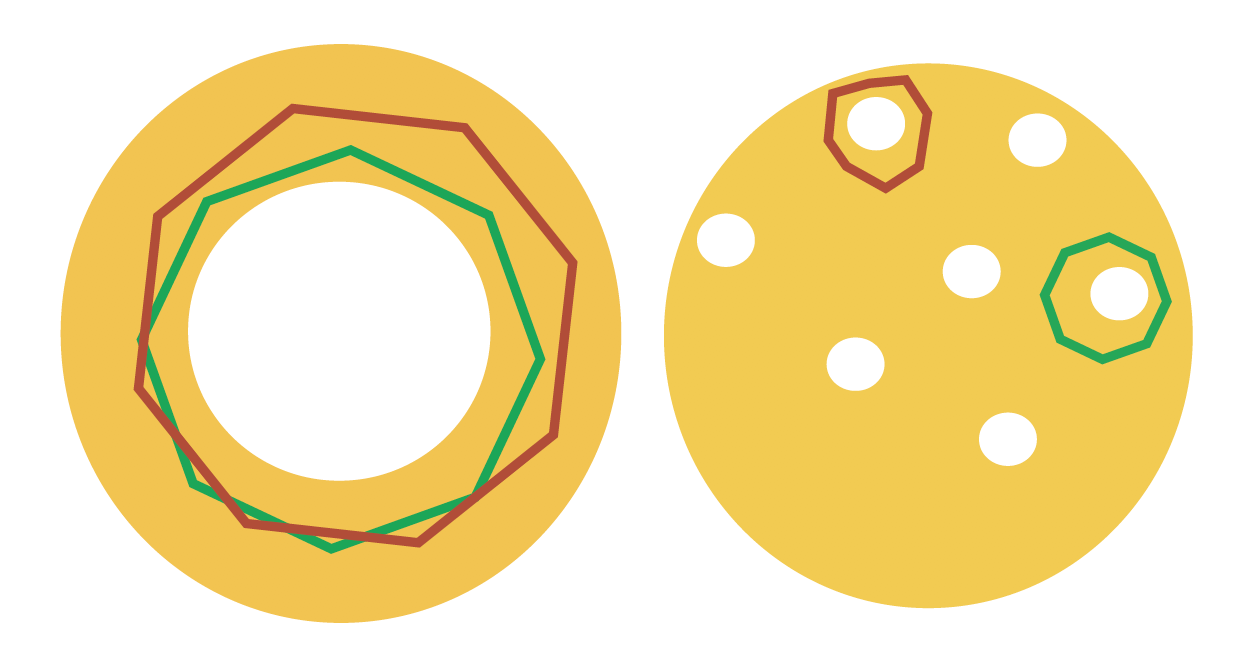
\includegraphics[width=0.8\textwidth]{figures/generatorExample.png}
    \caption{Two disks (yellow) --- which we regard as 2-dimensional simplicial complexes, though the explicit decomposition into simplices is not shown --- with different numbers of holes (white) and cycle representatives (red or green) from \cite{Carlsson2009TopologyAD}. The disk on the left has a single 2-dimensional  ``hole'' ($\beta_1 = 1$), and the two loops around it are cycle representatives for the same homology class. Similarly, the disk on the right has seven ``holes'' ($\beta_1 = 7$) and the two loops shown are cycle representatives for different homology classes.
    }
    \label{fig:generatorExamples}
\end{figure}


\begin{figure}[h!]
\begin{center}
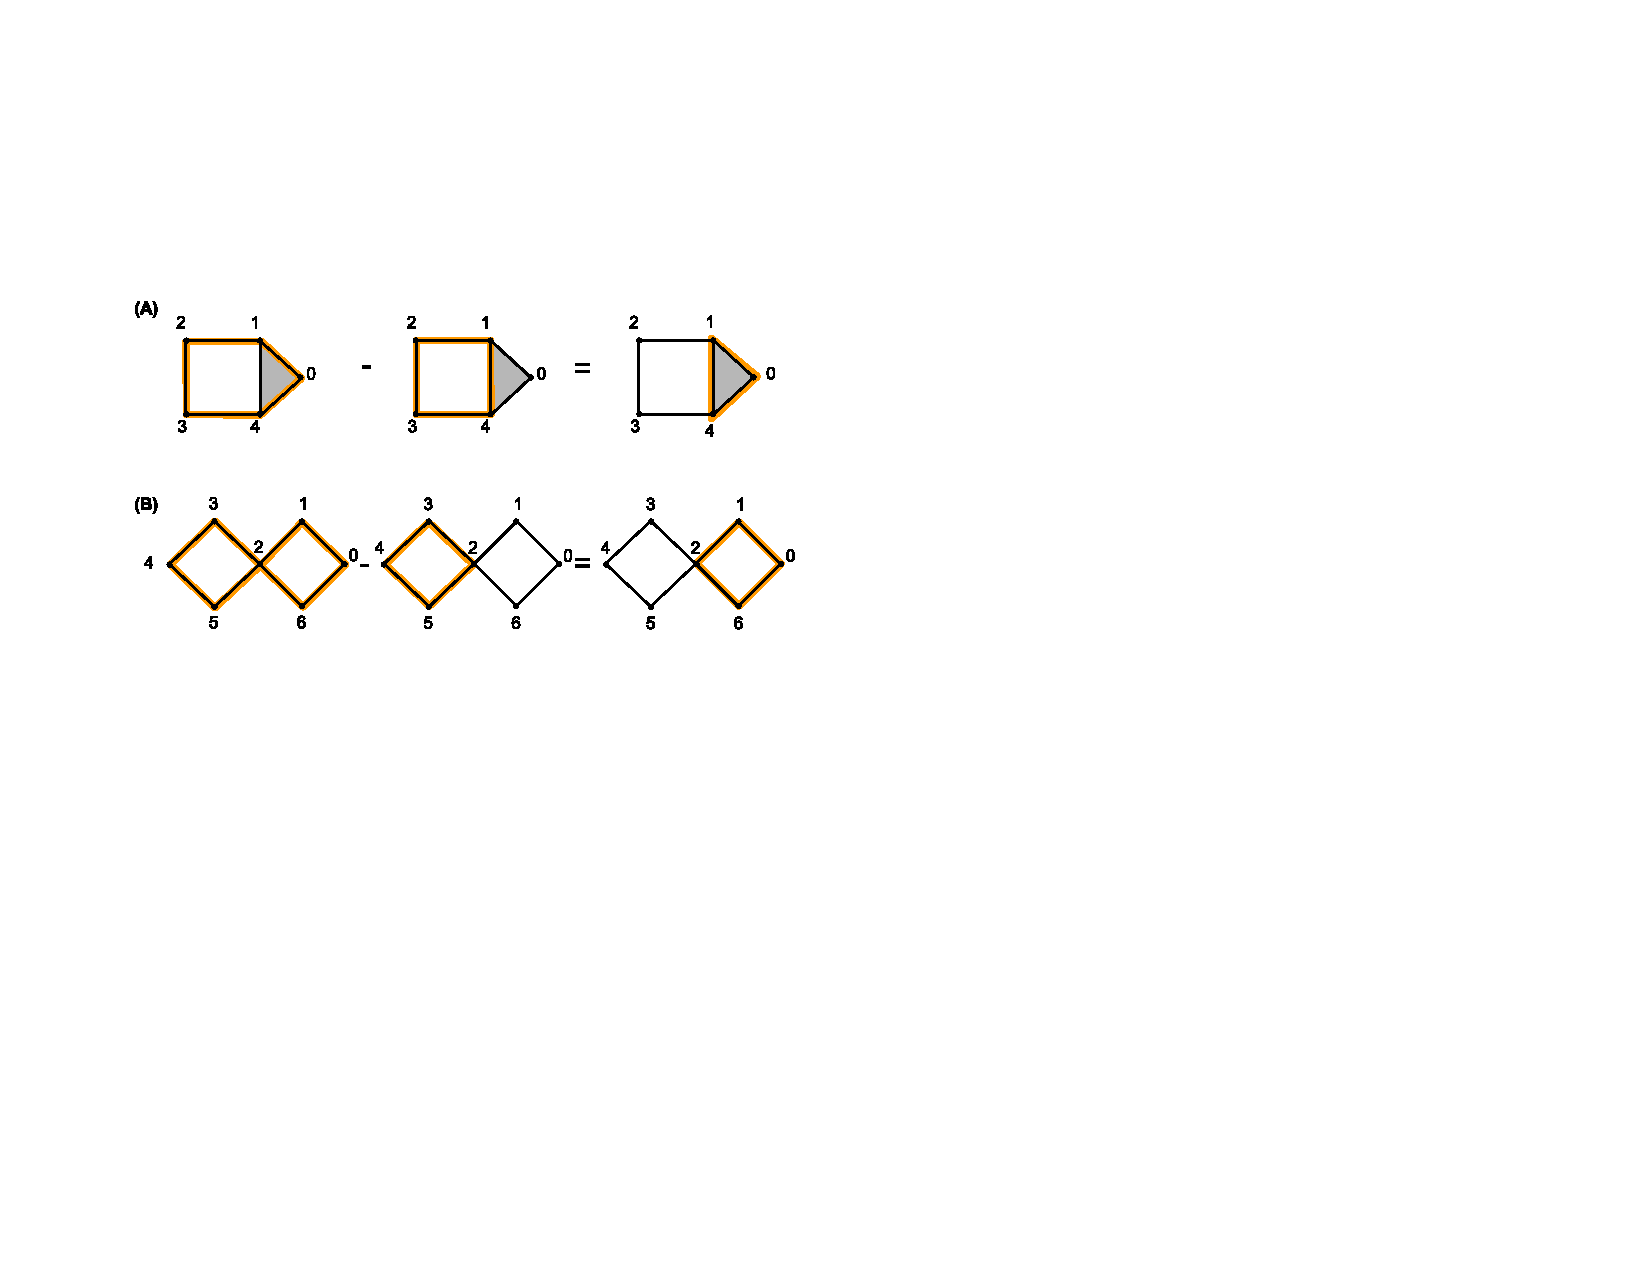
\includegraphics[width=1\textwidth]{figures/examplesorange.pdf}% This is a *.eps file
\end{center}
\caption{We show an example of homologous cycles in \textbf{(A)}, taken from \cite{TZH15}. The 1-cycle $(0,1) + (1,2) + (2,3) + (3,4) - (0,4)$ and the 1-cycle $(1,2) + (2,3) + (3,4) - (4,1)$ are homologous because their difference is the boundary of $(0,1,4)$. Subfigure \textbf{(B)} shows an example of non-homologous cycles. The 1-cycle $(\sum_{i=0}^4 (i, i+1))-(5,2)+(2,6)-(0,6)$ and the 1-cycle $(2,3) + (3,4)+(4,5)-(2,5)$ are not homologous because their difference is a cycle $(0,1)+(1,2)+(2,6)-(0,6)$ which is not a linear combination of boundaries of 2-simplices. } \label{fig:boundaryexample}
\end{figure}
% Section 3
\begin{figure}[h!]
\begin{center}
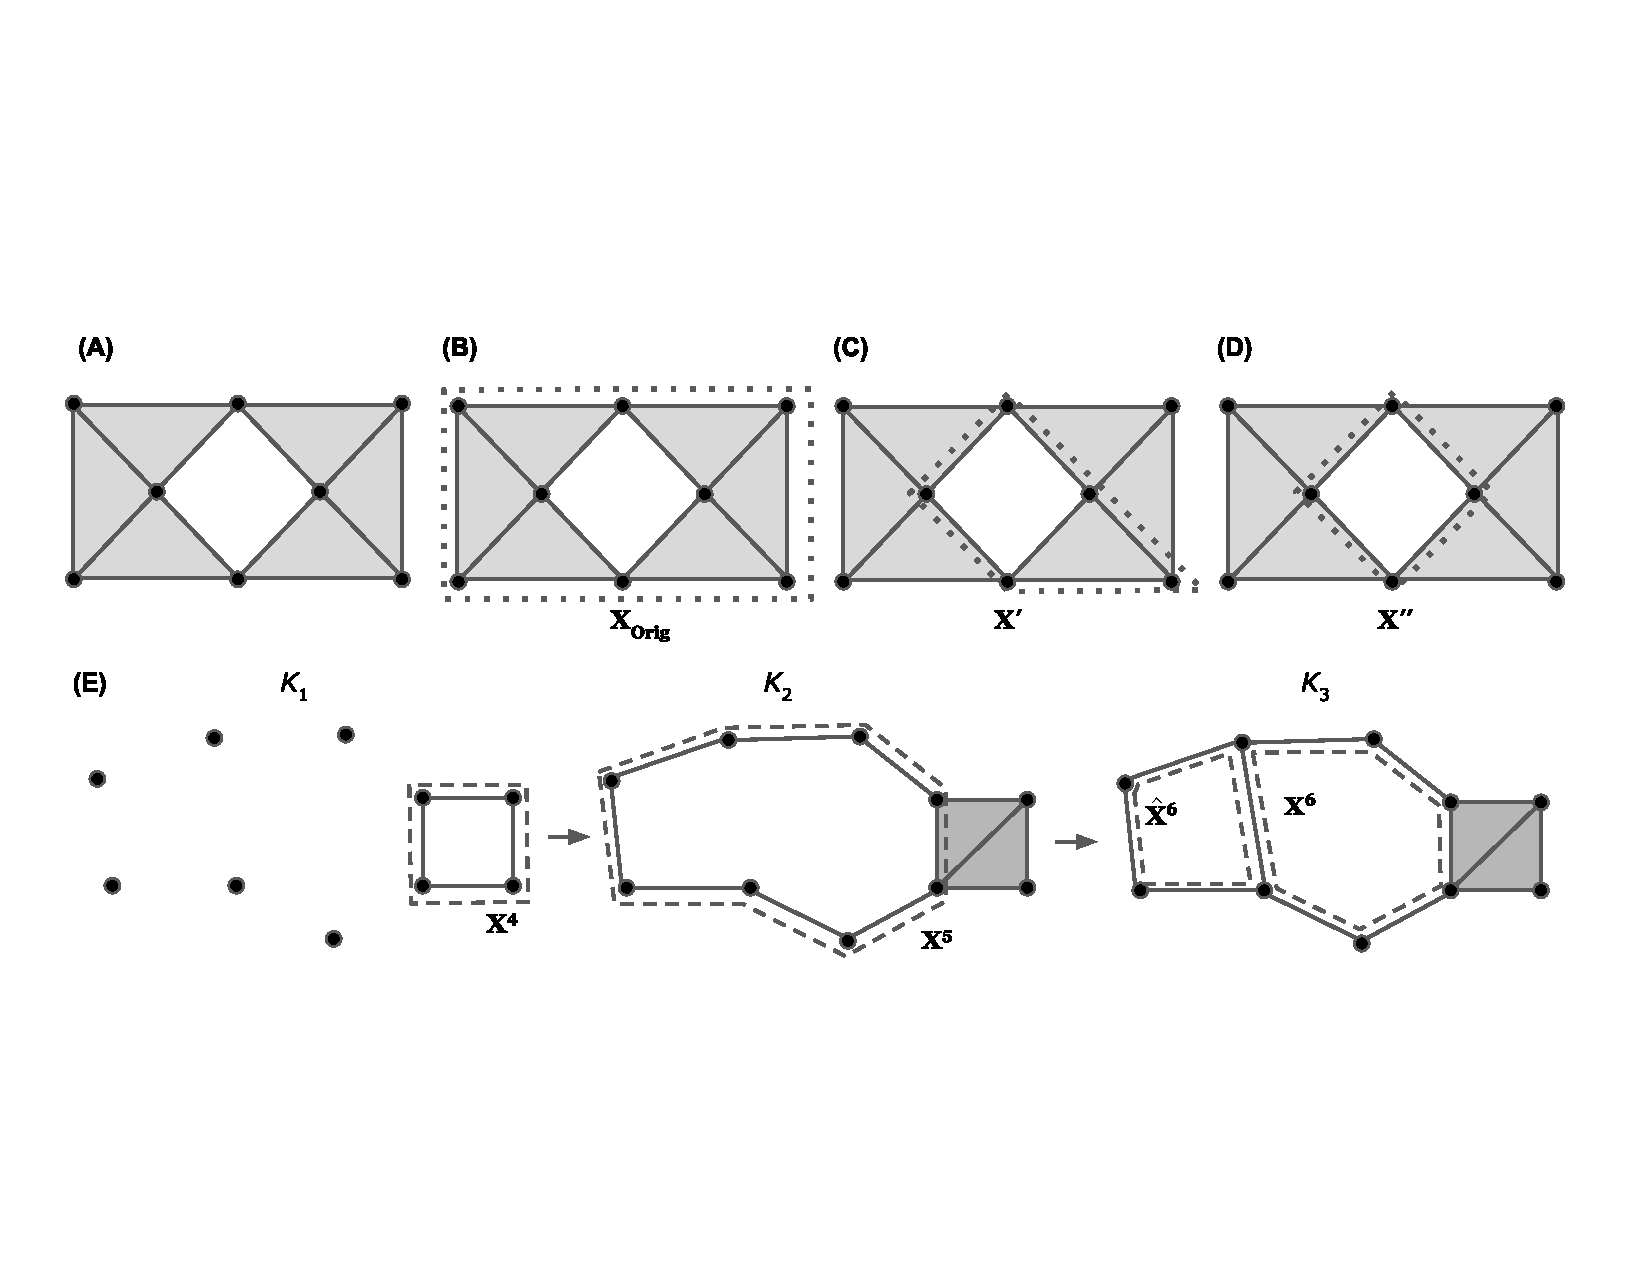
\includegraphics[width=1\textwidth]{figures/examplesminimal.pdf}% This is a *.eps file
\end{center}
\caption{Examples of optimizing a cycle representative (using the notion of minimizing edges) within the same homology class (\textbf{A-D}) and using a basis of cycle representatives (\textbf{E}), modified examples taken from \cite{Escolar2016} and \cite{Obayashi2018}. The dotted lines represent a cycle representative for the enclosed ``hole''. Intuitively, we consider $\optimalrep''$ in (\textbf{D}) as the optimal cycle representative since it consists of the smallest number of edges. Subfigure (\textbf{E}) shows a case where we optimize a cycle representative using a basis of cycle representatives. In (\textbf{E}), $\{\optimalrep^4, \optimalrep^5, \optimalrep^6\}$ is the original basis of cycle representatives. We can substitute $\optimalrep^6$ with $\hat{\optimalrep}^6$, which we can obtain by adding $\optimalrep^5$ to $\optimalrep^6$, and thus obtain $\{\optimalrep^4, \optimalrep^5, \hat{\optimalrep}^6\}$ as the new basis of cycle representatives.}\label{fig:example-optimal}
\end{figure}

\begin{figure}[h!]
\begin{center}
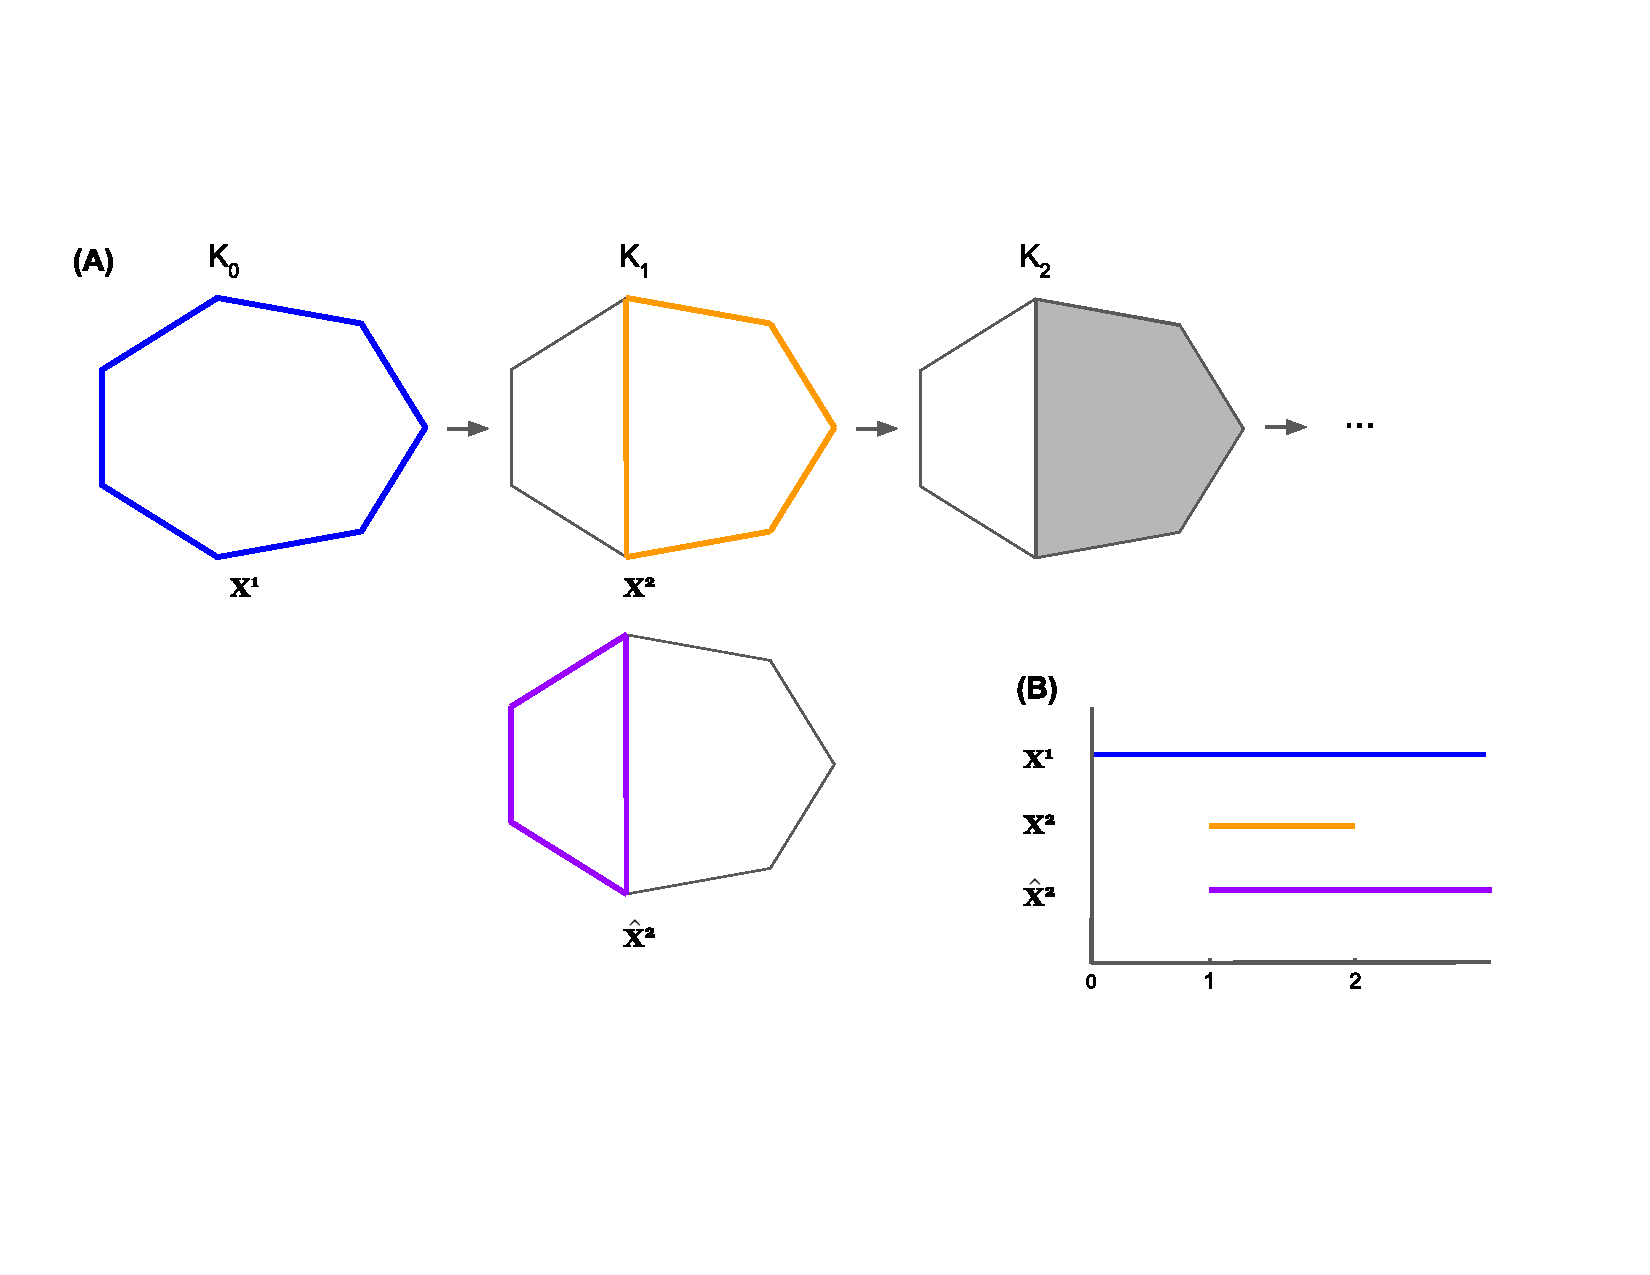
\includegraphics[width=1\textwidth]{figures/gregExample.pdf}% This is a *.eps file
\end{center}
\caption{An example where the optimal cycles obtained from \pr \eqref{eq:escolarargmin} do not form a persistent homological cycle basis. The thickened colored cycles in Subfigure (\textbf{A}) represent a cycle representative for the hole it encloses, and the bar with the corresponding color in Subfigure (\textbf{B}) records the lifespan of the cycle. In Subfigure (\textbf{A}), we see $\persinterval(\optimalrep^1) = [0,\infty), \persinterval(\optimalrep^2) = [1,2).$ Then, $\{\optimalrep^1, \optimalrep^2\}$ forms a basis for the persistent homological cycles. The cycle representative $\hat \optimalrep^2$ is an optimal cycle representative obtained by solving \pr (\ref{eq:filteredminimalbasis}) for the filtered simplicial complex $K_2$. However, $\persinterval(\hat \optimalrep_2) = [1, \infty)$, and thus  $\{\optimalrep^1, \hat \optimalrep^2\}$ is no longer a persistent homological cycle basis.} \label{fig:example-persBasis}
\end{figure}

\begin{figure}[h!]
\begin{center}
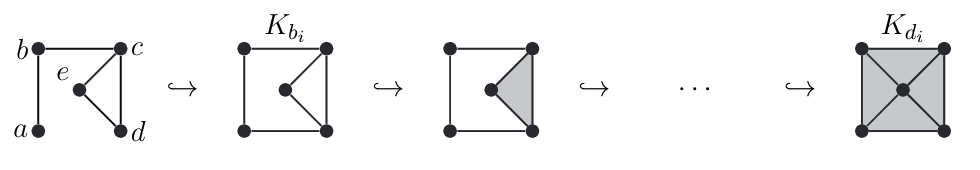
\includegraphics[width=1\textwidth]{figures/volumeexample.jpg}% This is a *.eps file
\end{center}
\caption{A situation in which a volume-optimal cycle is different from the uniform minimal cycle. Consider the filtered simplicial complex pictured. For the persistence interval $[b_i,d_i)$, the cycle with minimal $0$-norm (fewest number of edges) is $(a,b) + (b,c) + (c,d)  + (d,a)$.
However, the volume-optimal cycle would be found as follows: considering $K_{d_i}$, we must find the fewest $2$-simplices whose boundary captures the persistence interval. In this case, we would have an optimal volume $(a,b,e) + (b,c,e) + (a,d,e)$ and volume-optimal cycle $(a,b) + (b,c) + (c,e) + (e,d) + (d,a)$. 
}\label{fig:volumeoptimal}
\end{figure}
% section 4
%
 \begin{figure}[h!]
 \begin{center}
 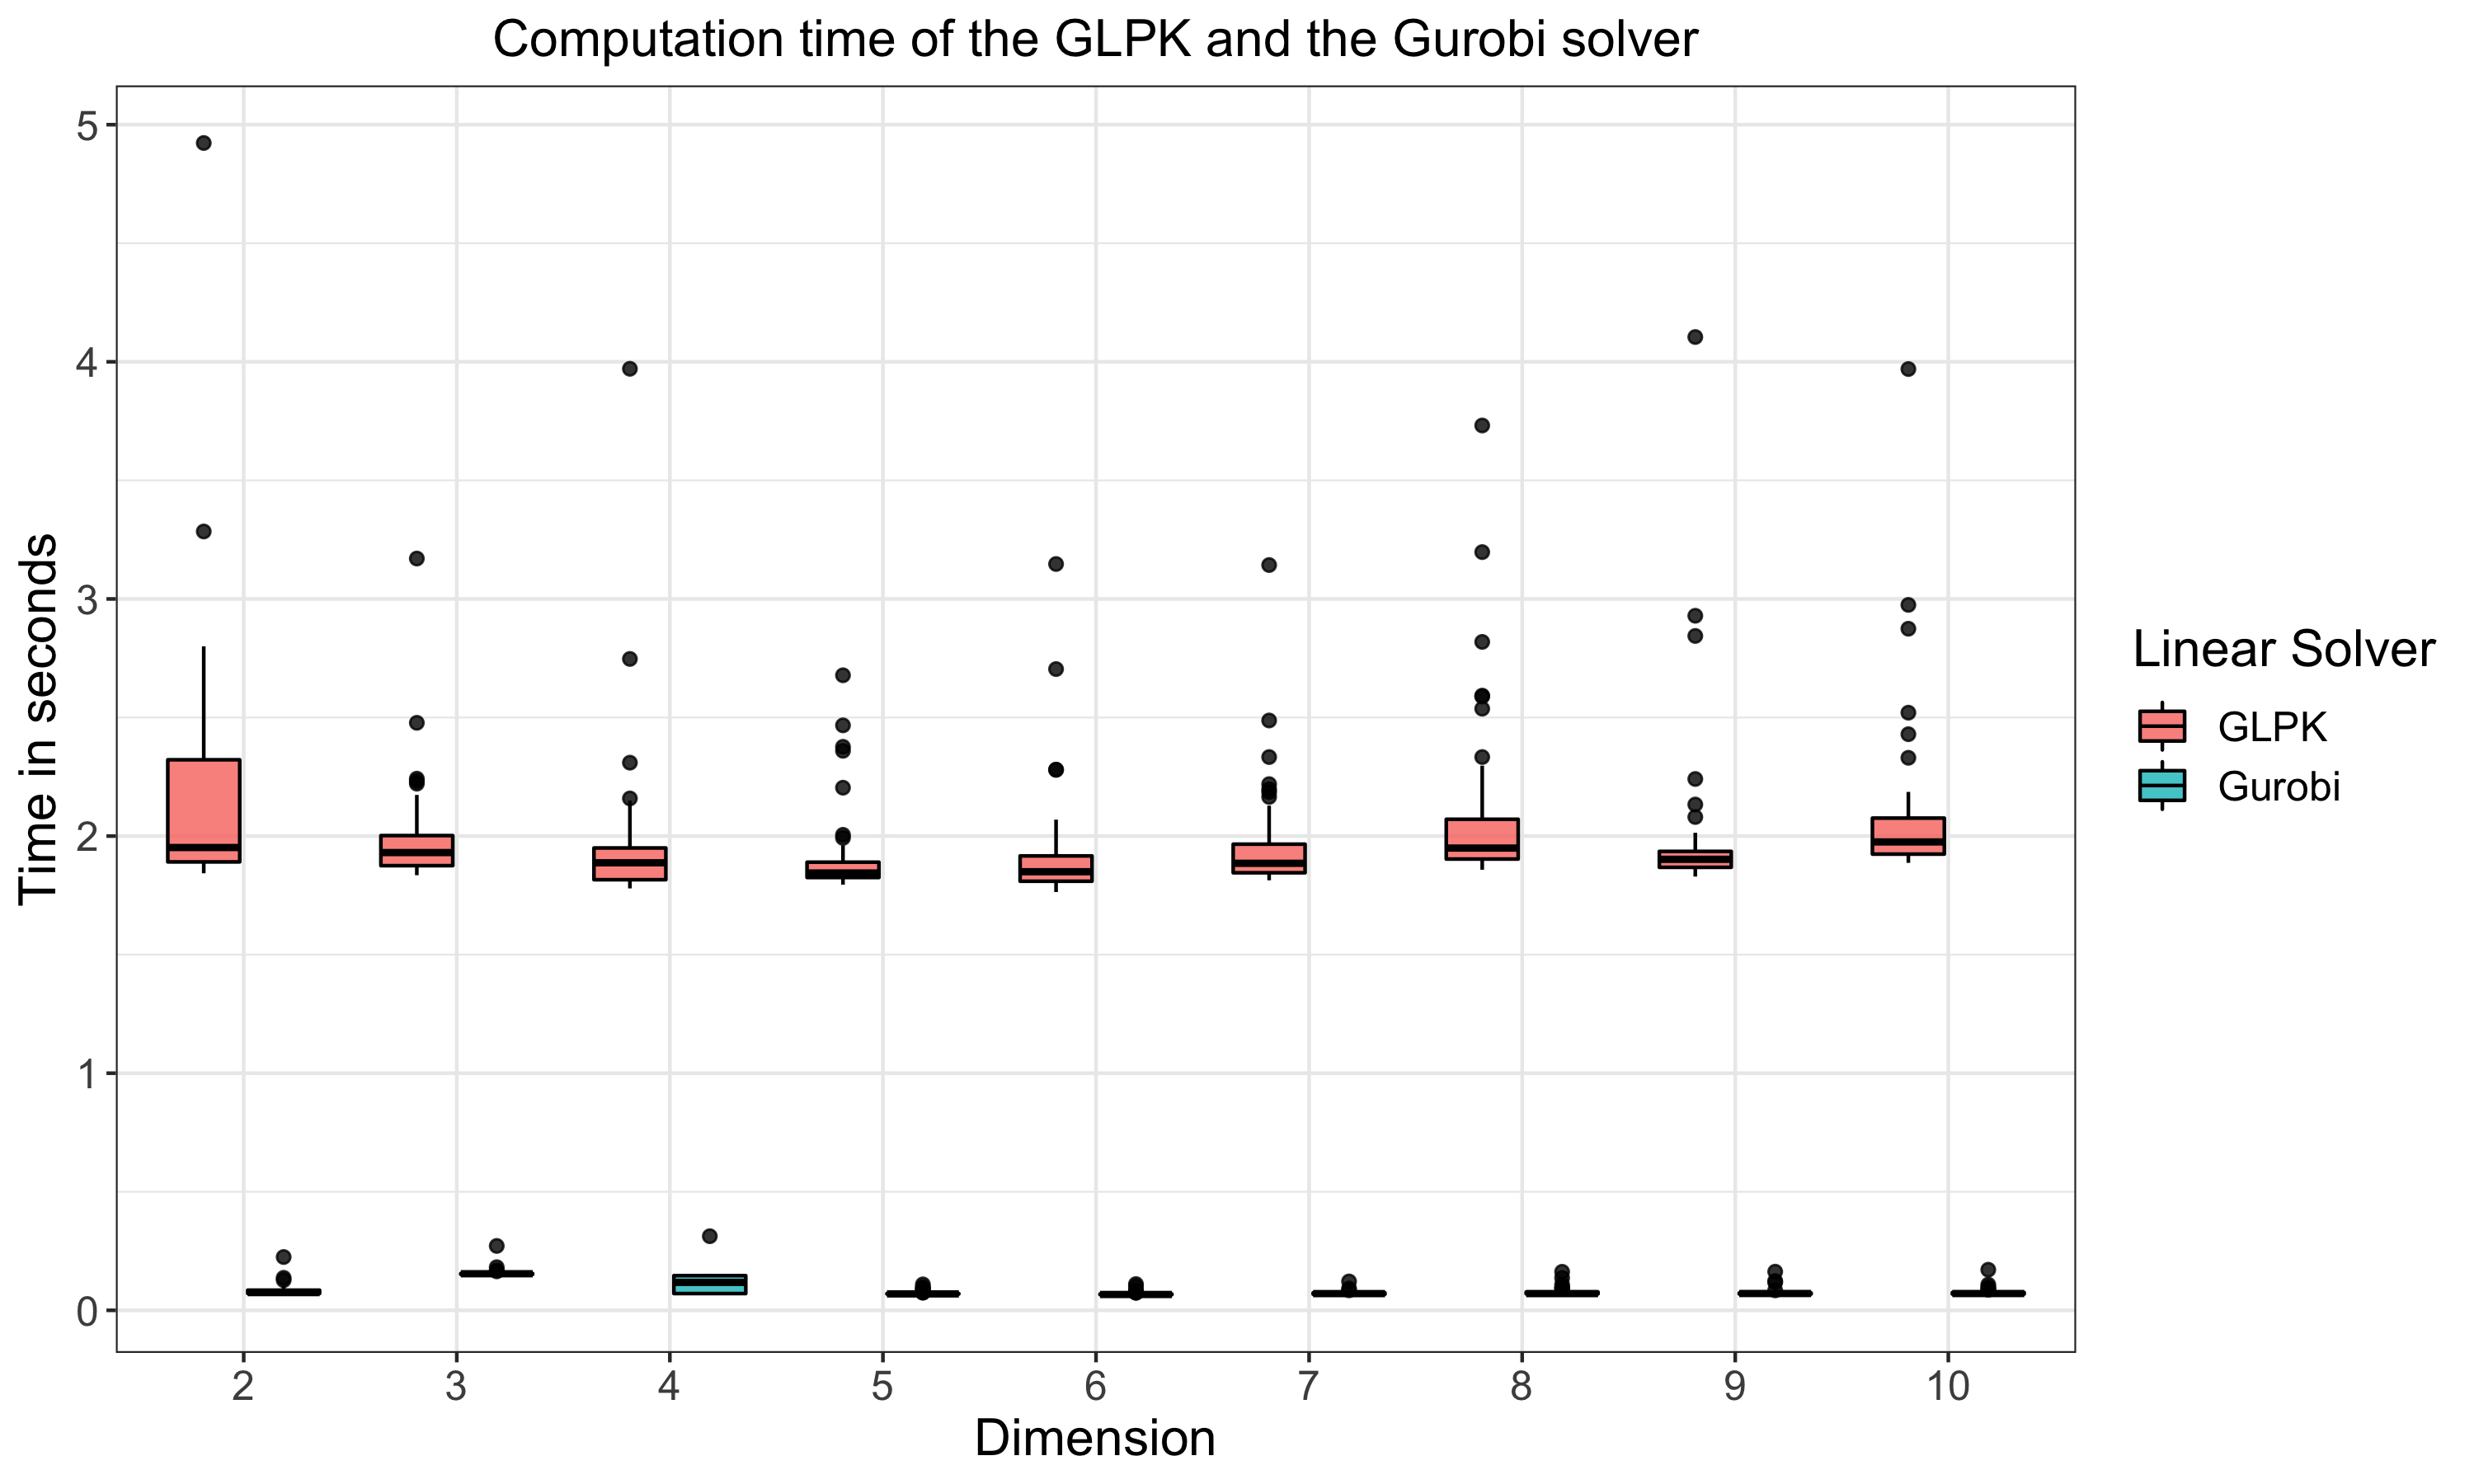
\includegraphics[width=1\textwidth]{boxplots_glpk_gurobi.jpg}% This is a *.eps file
 \end{center}
 \caption{Computation time of the GLPK linear solver (red) and the Gurobi linear solver (green) to solve the uniform/length-weighted edge-loss minimal problems in Algorithm 1. We perform experiments on $90$ data sets, 10 for each dimension 2-10, generated from the normal distribution. The horizontal axis is the dimension of the data set, and the vertical axis is the time it takes to solve an optimization problem. We observe that the Gurobi solver is consistently faster than the GLPK solver and that computation time seems fairly constant across dimension.}\label{fig:glpk_gurobi}
 \end{figure}

% % \begin{figure}[h!]
% % \begin{center}
% % 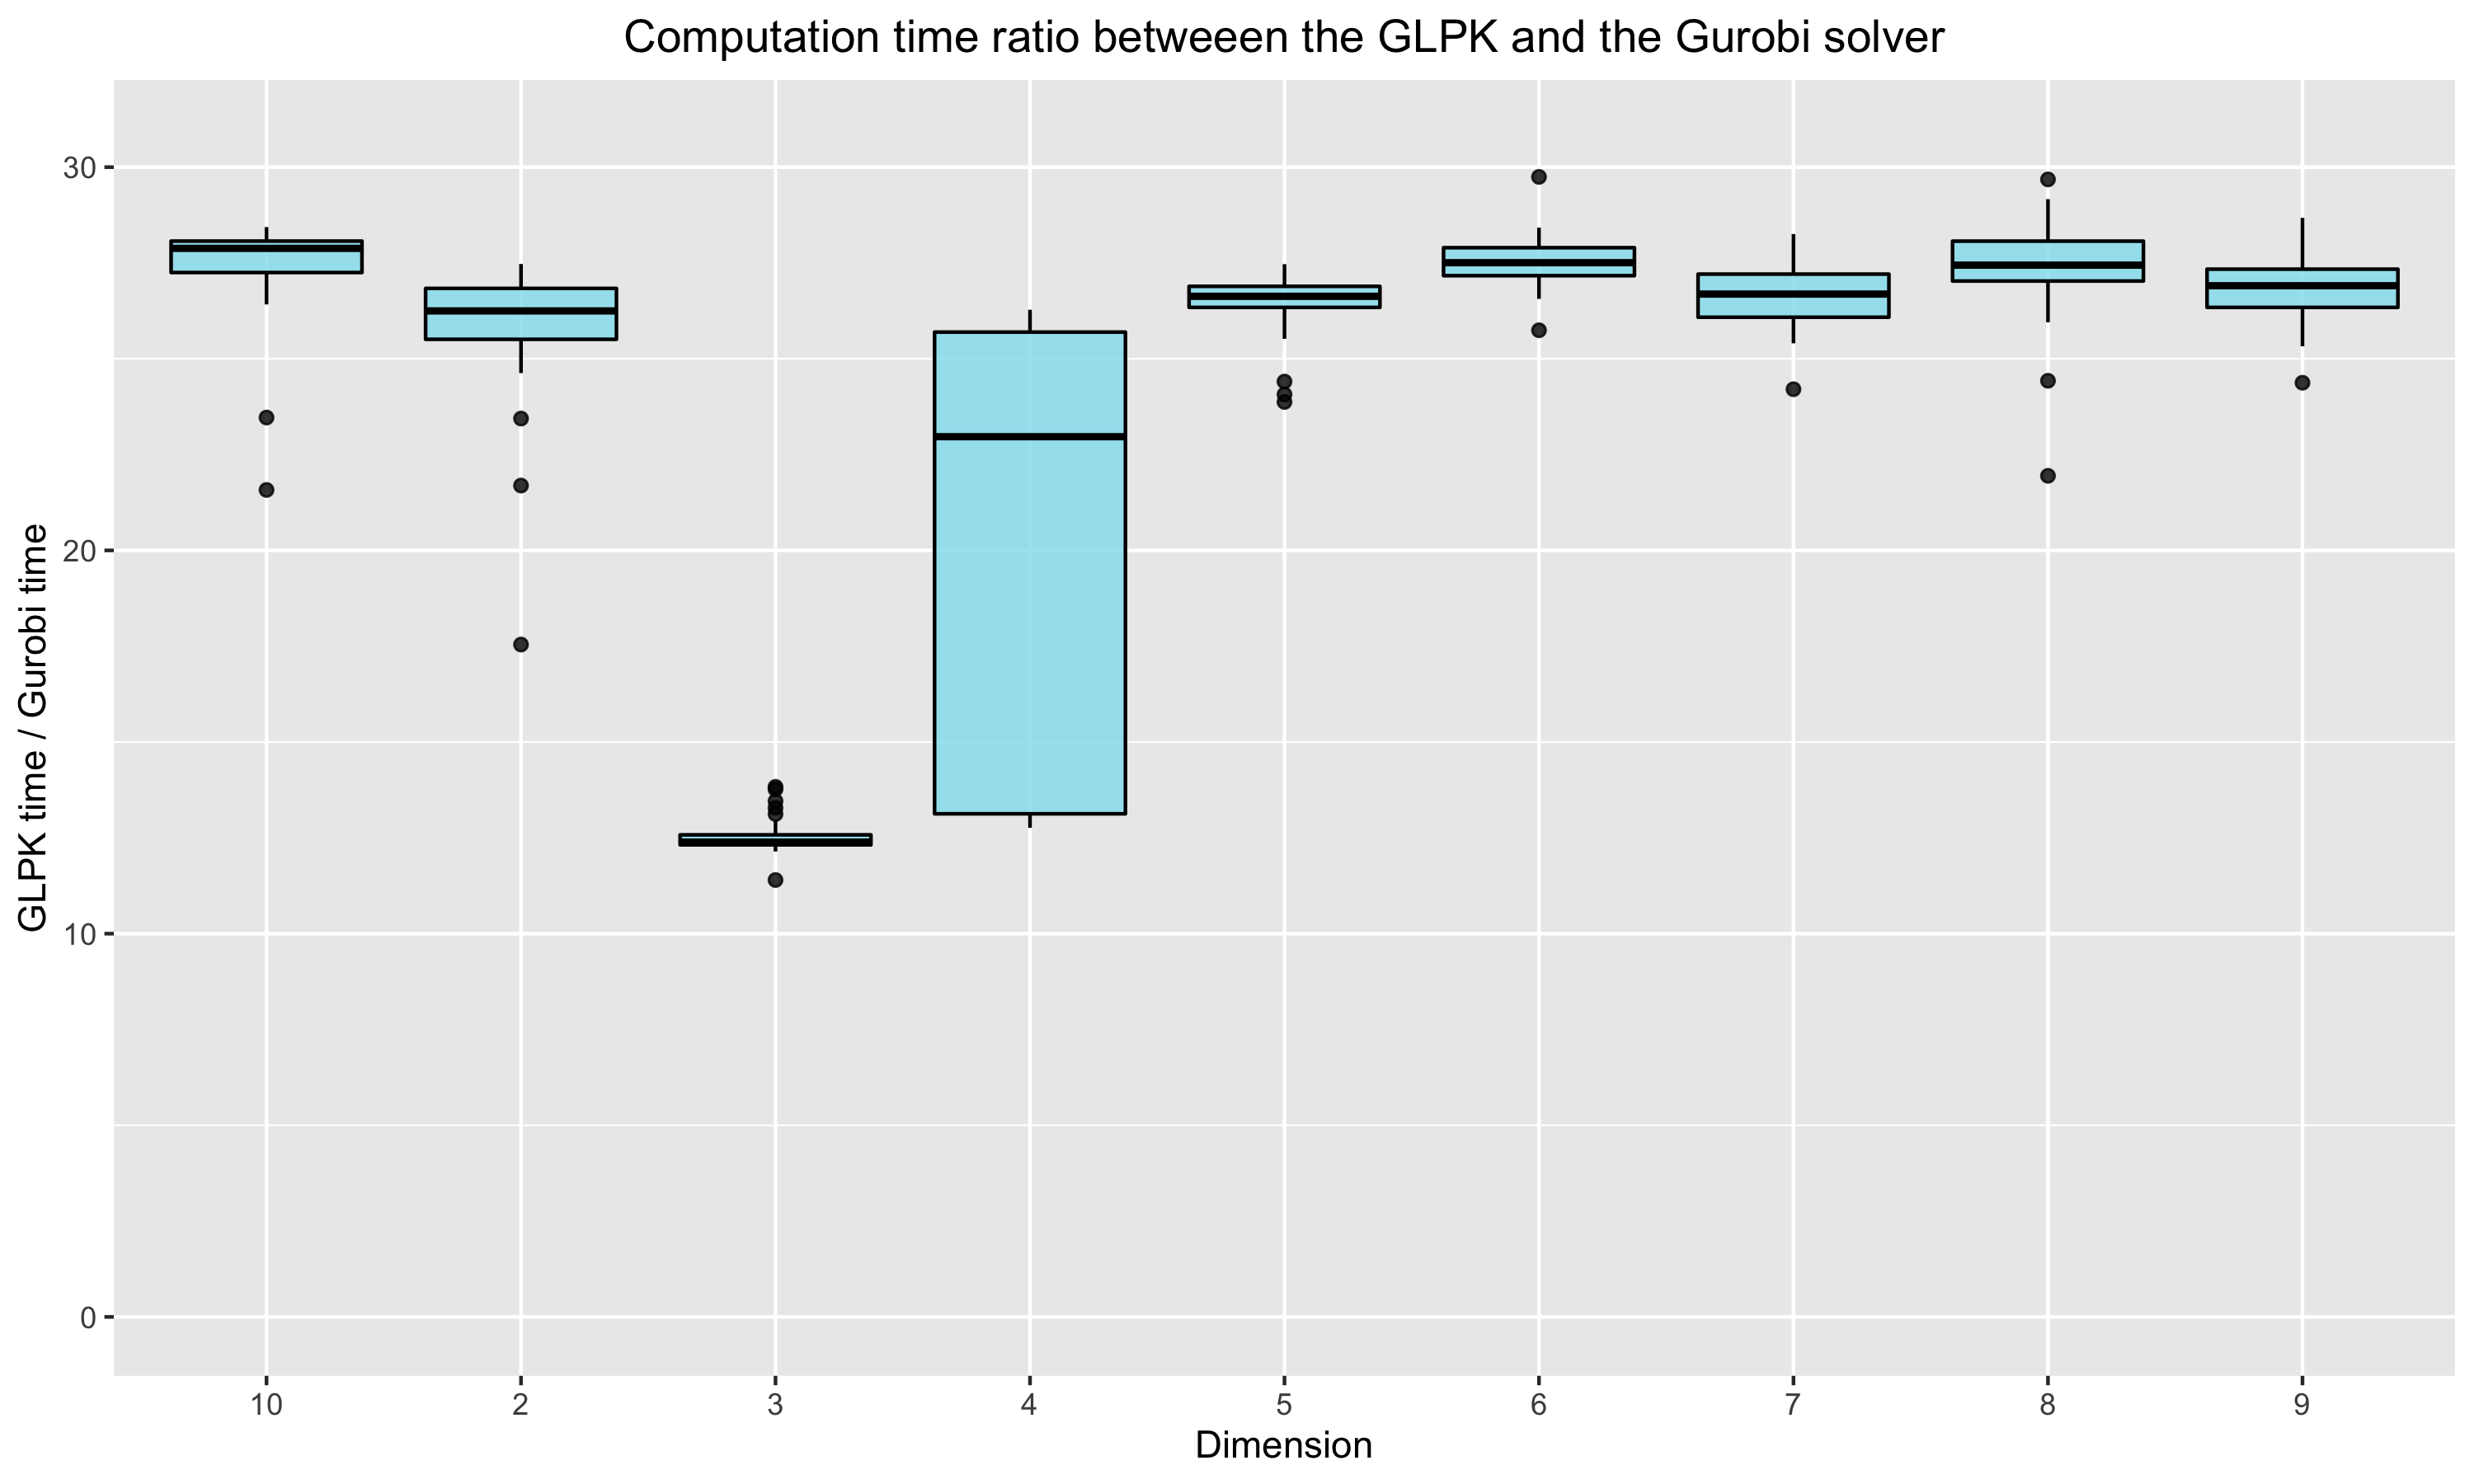
\includegraphics[width=1\textwidth]{figures/computationratio_glpk_gurobi.png}% This is a *.eps file
% % \end{center}
% % \caption{Computation time ratio of the GLPK and Gurobi linear solver. We observe that the Gurobi solver can be a lot faster than the GLPK solver.}\label{fig:glpk_gurobi}
% % \end{figure}


% section 6
\begin{figure}[h!]
\begin{center}
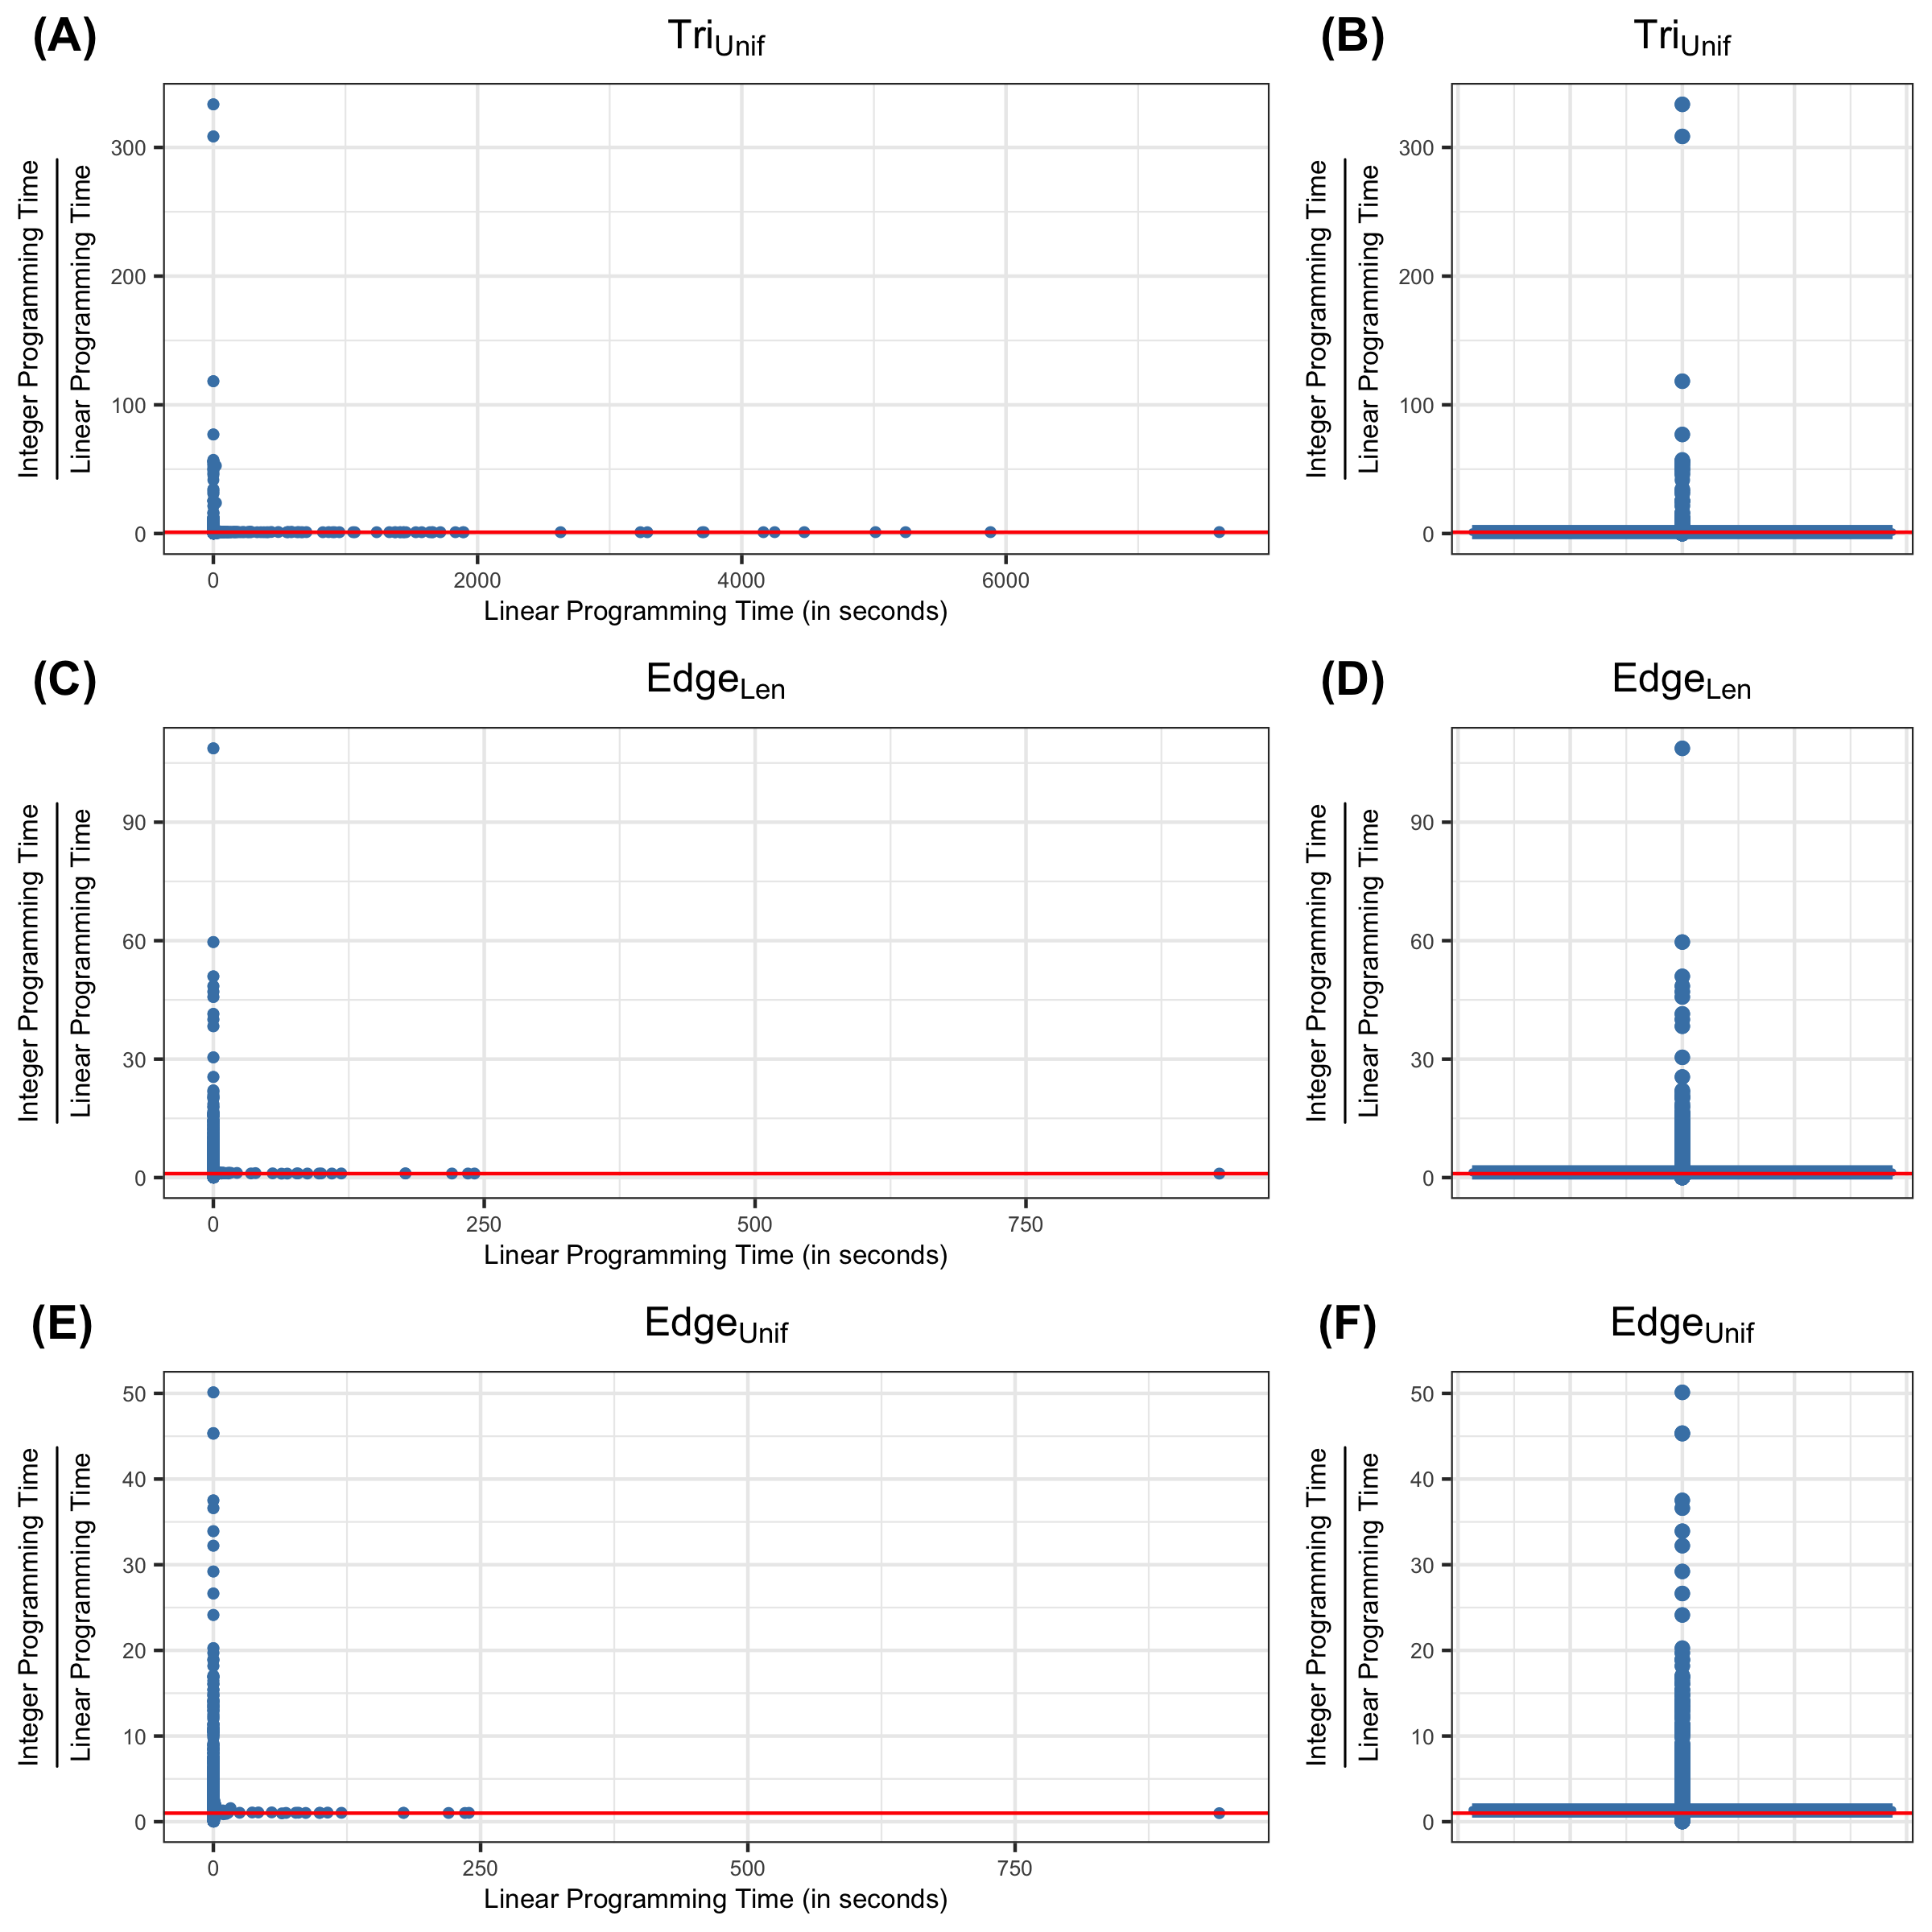
\includegraphics[width=\textwidth]{figures/IPvsLP.png}% This is a *.eps file
\end{center}
 \caption{
%  \GHP{Delete the phrase ``This figure shows the'' in every figure caption. }
 Ratio between the computation time of solving an integer programming problem Programs \ref{itm:tri_IU},\ref{itm:edge_IL}, \ref{itm:edge_IU} and the computation time of solving a linear programming problem Programs \ref{itm:tri_NIU},\ref{itm:edge_NIL}, \ref{itm:edge_NIU} for all the cycle representatives from data sets described in \se \ref{tab:realworldata} and \se \ref{tab:distributiondata}. Subfigures  \textbf{(A), (C), (E)} plot the data using scatter plots and subfigures  \textbf{(B), (D), (F)} show the same data using box plots. The vertical axis represents the ratio between the integer programming time and linear programming time of optimizing a cycle representative and the horizontal axis represents the computation time to solve the linear program. The red line in each subfigure represents the horizontal line $y=1$, where the time for each optimization is equivalent. As we can see from the box plots, the ratio between the computation time of integer programming and linear programming for most of the cycle representatives ($>50\%$) center around $1$.}\label{fig:lp_mip_ratio_df}
\end{figure}
% \begin{figure}[h!]
% \begin{center}
% 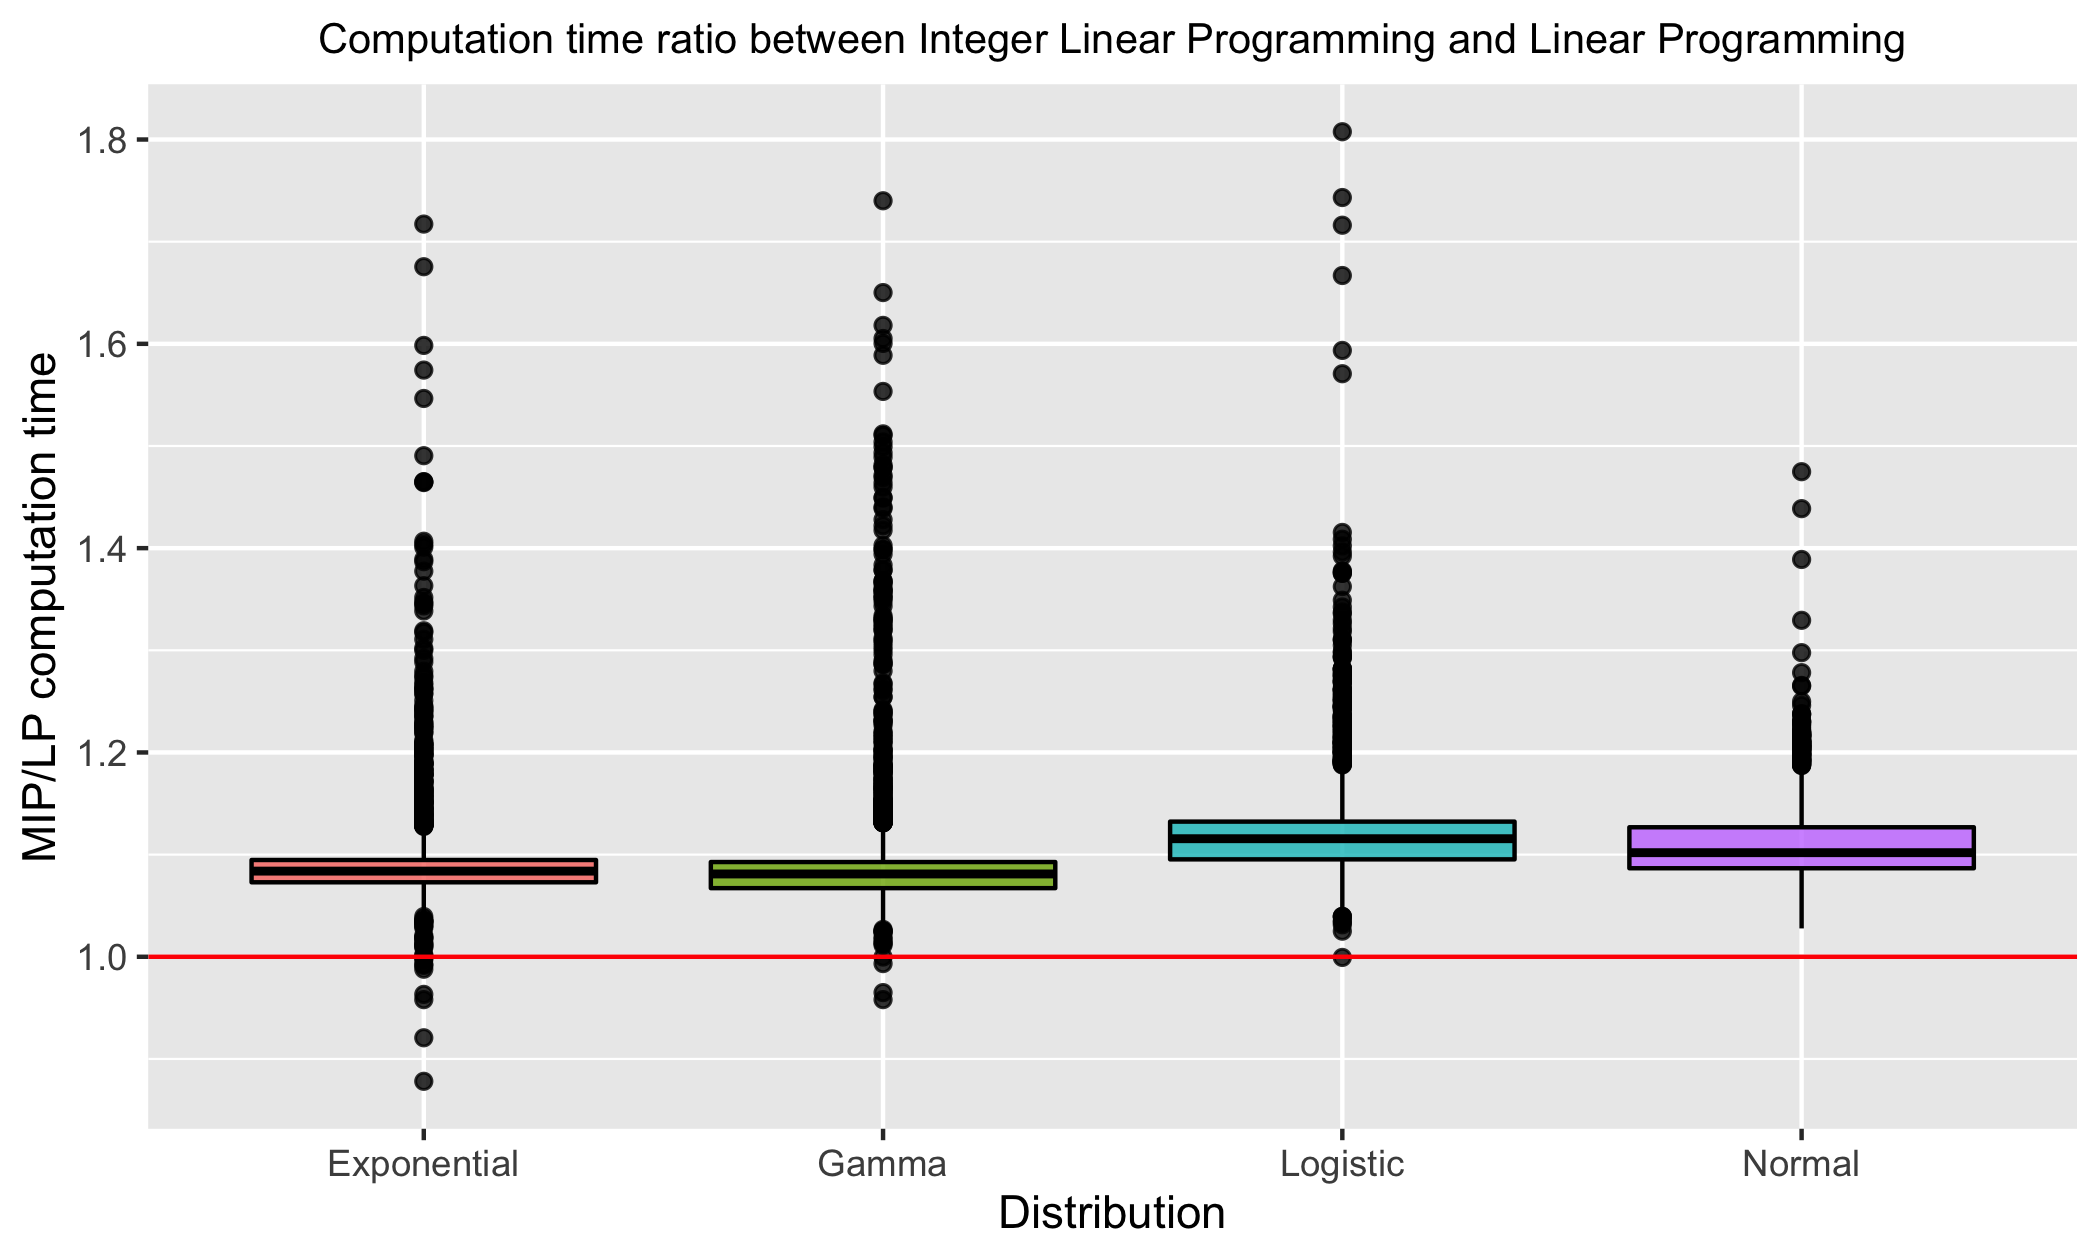
\includegraphics[width=0.8\textwidth]{figures/comptime_dist.png}% This is a *.eps file
% \end{center}
% \caption{Computation time ratio between integer programming and linear programming for randomly generated data sets. The x-axis is the distribution, and the y-axis is the ratio between the computation taken between requiring integer solutions and not requiring integer solutions. The red line marks the the value of 1. Linear programming was almost always faster than integer linear programming, although none of the displayed ratios exceed 2.0. }\label{fig:lp_mip_ratio_dist}
% \end{figure}

% delete legend 
% make x,y,title labels larger
\begin{landscape}
\begin{figure}[hbt!]
\begin{center}
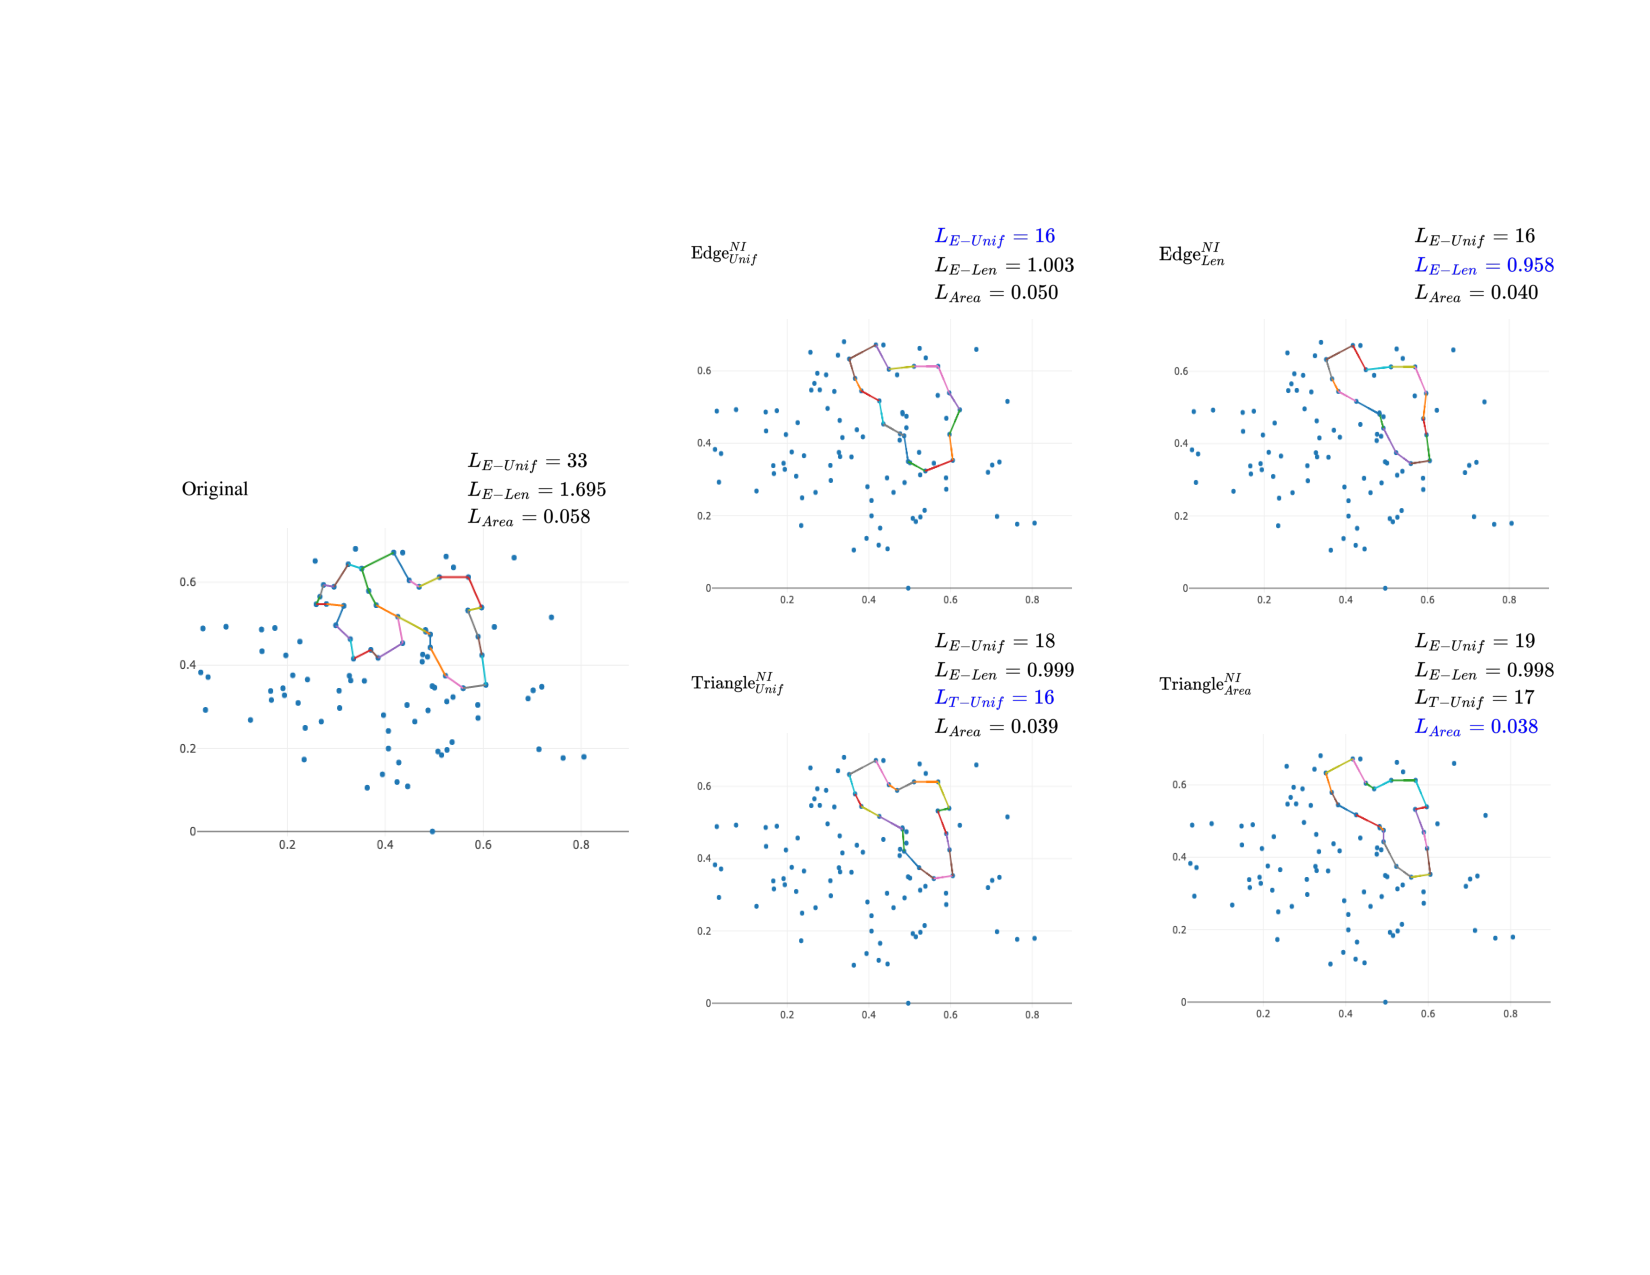
\includegraphics[width=\textwidth]{figures/examples.pdf}
\end{center}
\caption{Examples of different optimal cycles and cost against different loss functions using a point cloud of $100$ points with ambient dimension $2$ randomly drawn from a normal distribution. The upper left corner of each subfigure labels the optimization algorithm used to optimize the original cycle representative. The upper right corner of each subfigure records the different measures of the size of the optimal representative. Blue text represents the measure an algorithm sets out to optimize. 
}\label{fig:Examplesofeachoptimalcycles} 
\end{figure}
\end{landscape}
% \textbf{(A)} is the original cycle, \textbf{(B)} is the uniform-weighted minimal cycle, \textbf{(C)} is the length-weighted minimal cycle, \textbf{(D)} is the volume, \textbf{(E)} is the area optimal cycle.

% \vspace{0.1in}

% \begin{table}[hbt!]
%     \centering
%     \begin{tabular}{ |c || c |c |c |c |}
%  \hline
%  & Length & Edge  & Area & Volume  \\[0.5ex] 
%  \hline 
%  $X_{Orig}$ & 1.695 & 33  & 0.0576 &  -  \\\hline  

% $X_{Len}$ &  \textbf{0.0958} &  16  &  0.0398 &   -  \\\hline  
% $X_{Unif}$ & 1.003 & \textbf{16}   & 0.0496 &  -  \\\hline  

% $X_{Area}$ &   0.998  & 19  & \textbf{0.038 }& 17  \\  \hline
% $X_{Vol}$ &   0.999  & 18    & 0.0391 & \textbf{16} \\ \hline

% \end{tabular}
% \caption{Summary of the example in Figure \ref{fig:volumeExample}}
% \label{tab:data}
% \end{table}

\begin{figure}[h!]
\begin{center}
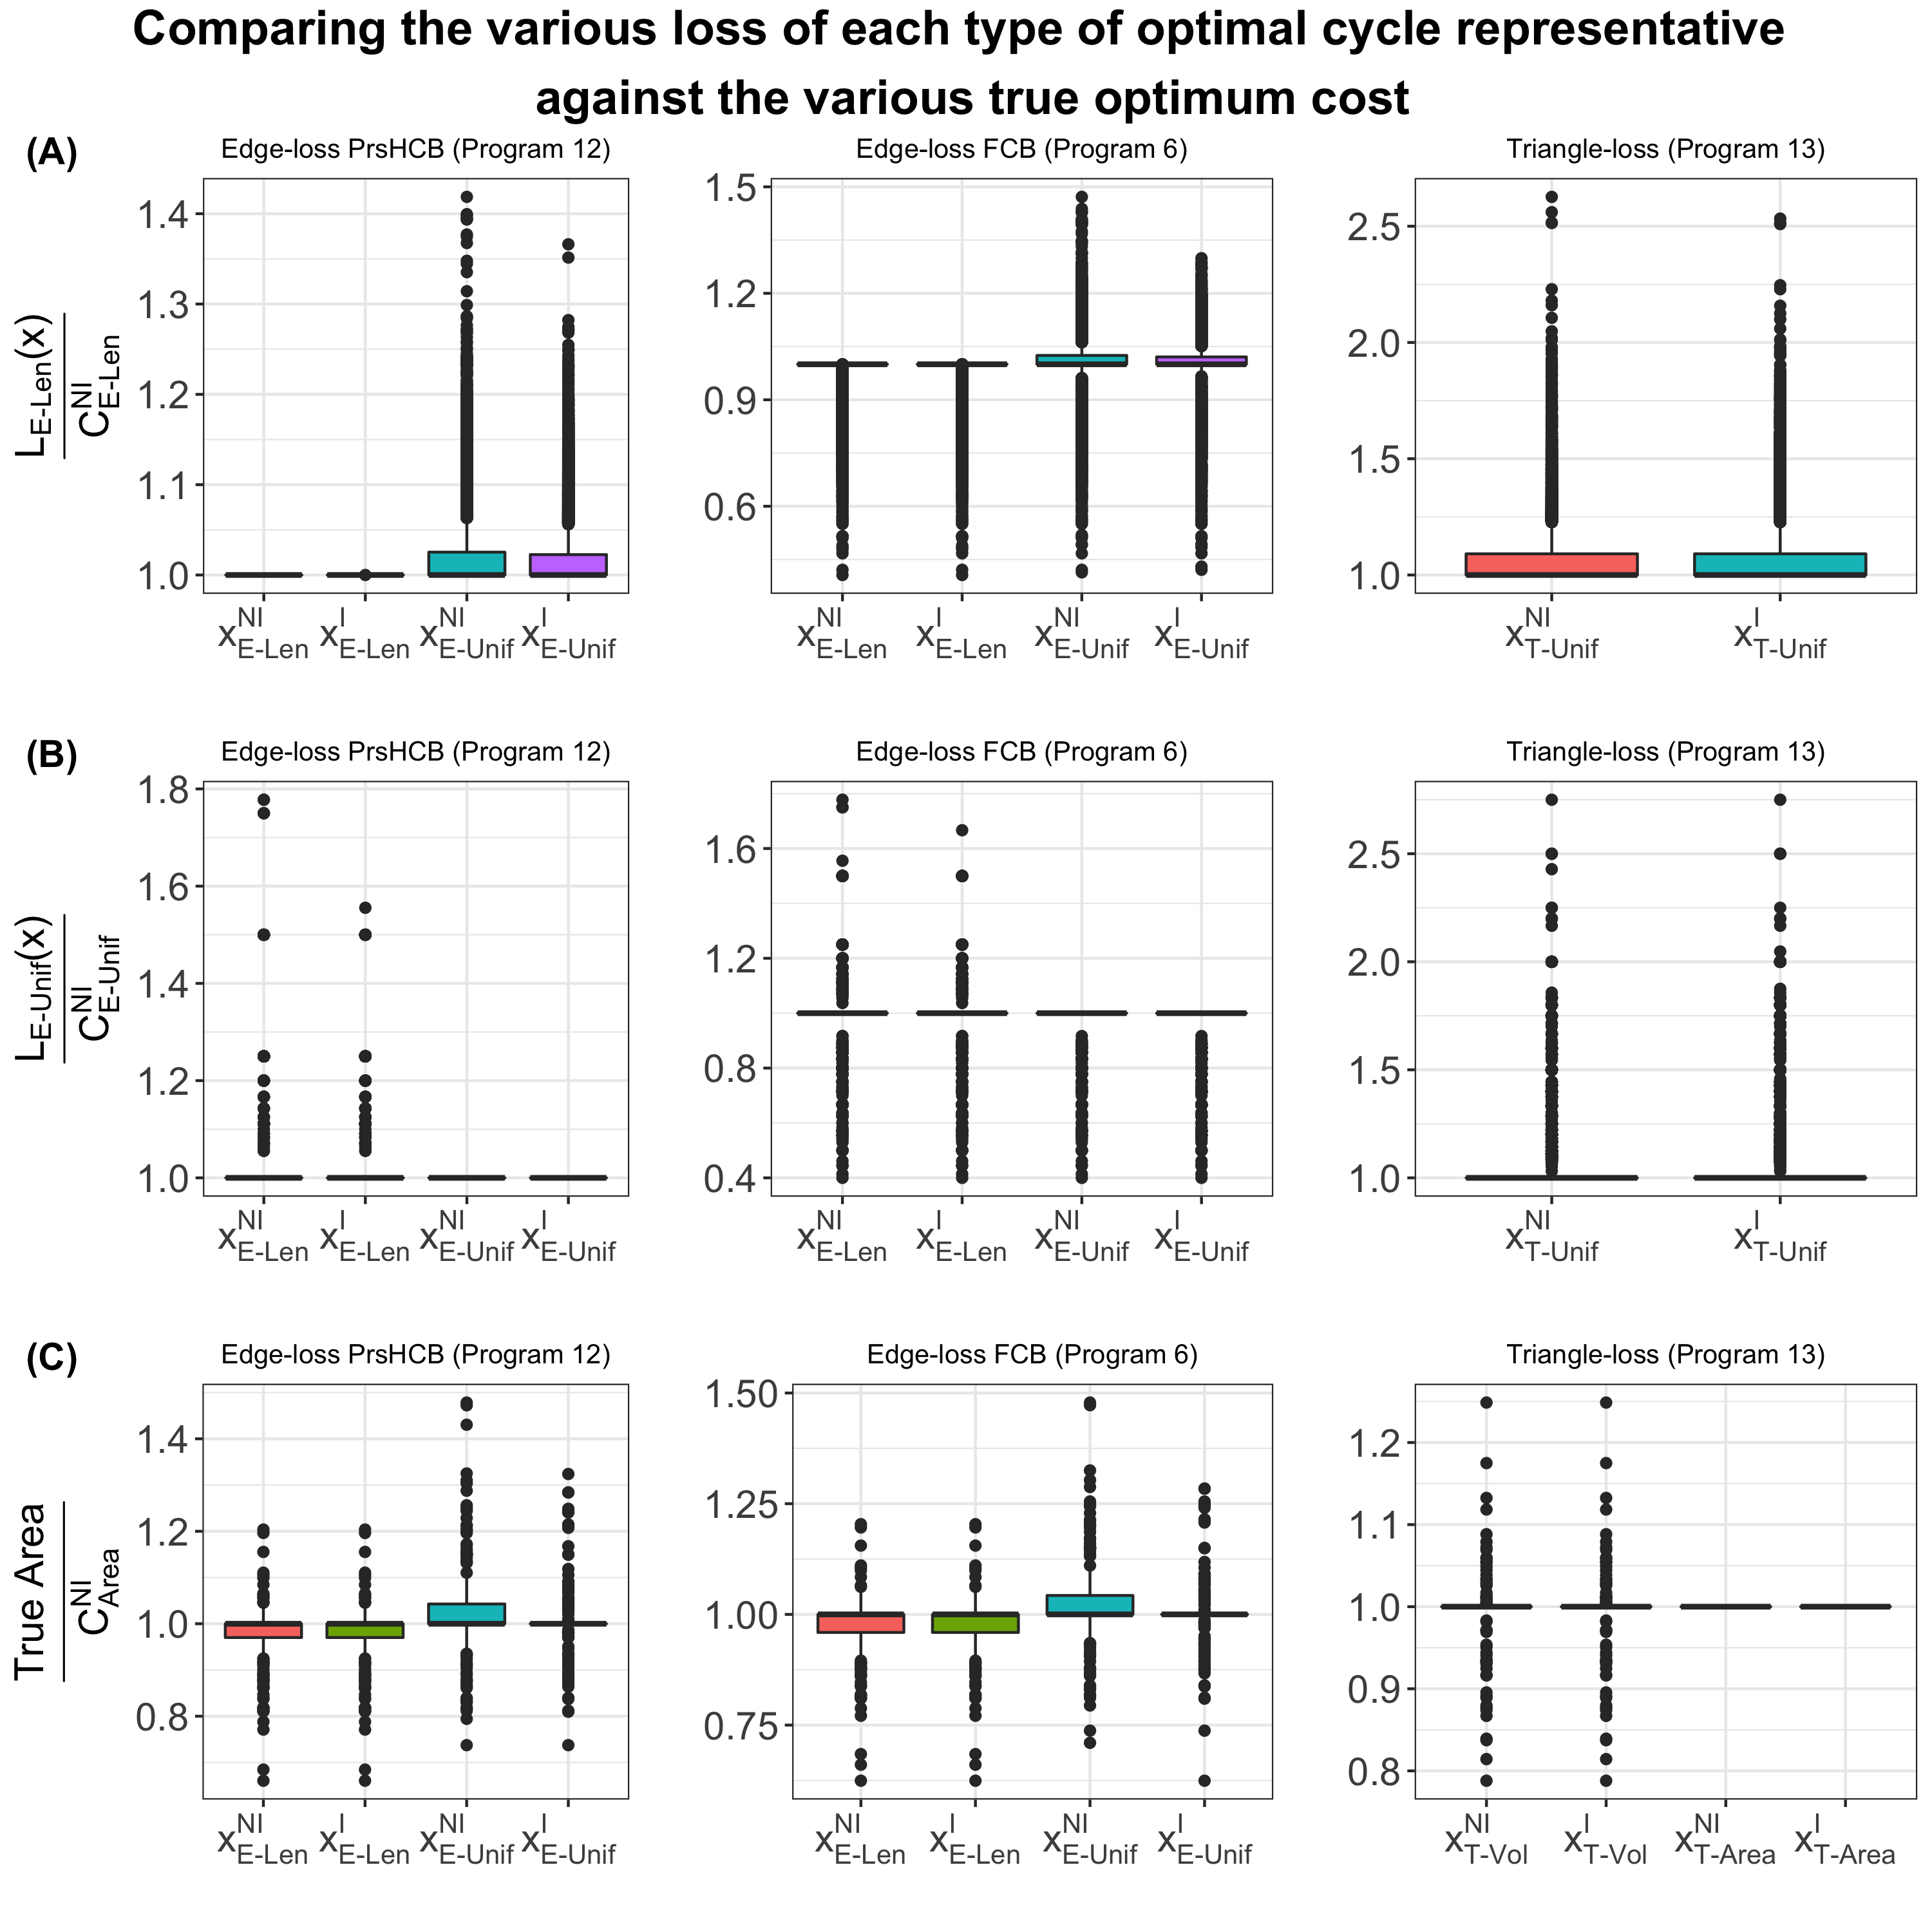
\includegraphics[width=\textwidth]{figures/length_area_edge.png}
\end{center}
\caption{Box plots of the ratios between (\textbf{A}) $L_{E\text{-}Len}(\optimalrep_\bullet^\bullet)$ and $C_{E\text{-}Len}$,  \textbf{(B)} $L_{E\text{-}Unif}(\optimalrep_\bullet^\bullet)$ and $C_{E\text{-}Unif}$, and  \textbf{(C)} $L_{T\text{-}Area}(\optimalrep_\bullet^\bullet)$ and $C_{T\text{-}Area}$. 
The horizontal axis is the type of optimal representative, $\optimalrep_\bullet^\bullet$, and the vertical axis is the ratio between the loss of each type of optimal representative over the actual cost of the optimal representative of the same loss function, i.e. the $\setofpersistenthcyclebases$ cycles which are solutions to Programs \ref{itm:edge_NIU}, \ref{itm:edge_NIL}, \ref{itm:tri_NIA}.
In \se \ref{coefficient}, we discussed that the optimum cost is the same whether we require an integer solution or not for essentially all solutions for \pr \eqref{eq:edgelossgeneral}, \pr \ref{eq:escolarargmin}, and the uniform-weighted triangle-loss method, resulting in two columns in the first two rows having ratio 1. The data used in \textbf{(A)} and \textbf{(B)} aggregate over all data described in \ref{sec: realworlddata} and \ref{sec: randompointclouds}. The data used in \textbf{(C)} aggregate the $190$ cycle representatives from $10$ point clouds from a normal distribution with ambient dimension of $2$. True area represents the total area enclosed by the representative, while $C_{Area}\NI$ represents the area of the area-weighted triangle-loss optimal cycle minimizing \ref{itm:tri_NIA}. We observe that some edge-loss optimal cycles and triangle-loss optimal cycles requiring integral solutions have an area smaller than that of the area-weighted triangle-loss optimal cycle. Refer to Figure \ref{fig:areaExample} and \se  \ref{sec:comparing optimal generators against different loss functions} to see why this may happen. 
% In addition to $\optimalrep_{Area}\NI = \optimalrep_{Area}\I$ for corresponding cycle representatives in all experiments, so too are $\optimalrep_{Len}\NI = \optimalrep_{Len}\I$.
}
 \label{fig:lengthcocmpare}
\end{figure}


 %\begin{figure}[h!]
%\begin{center} 
%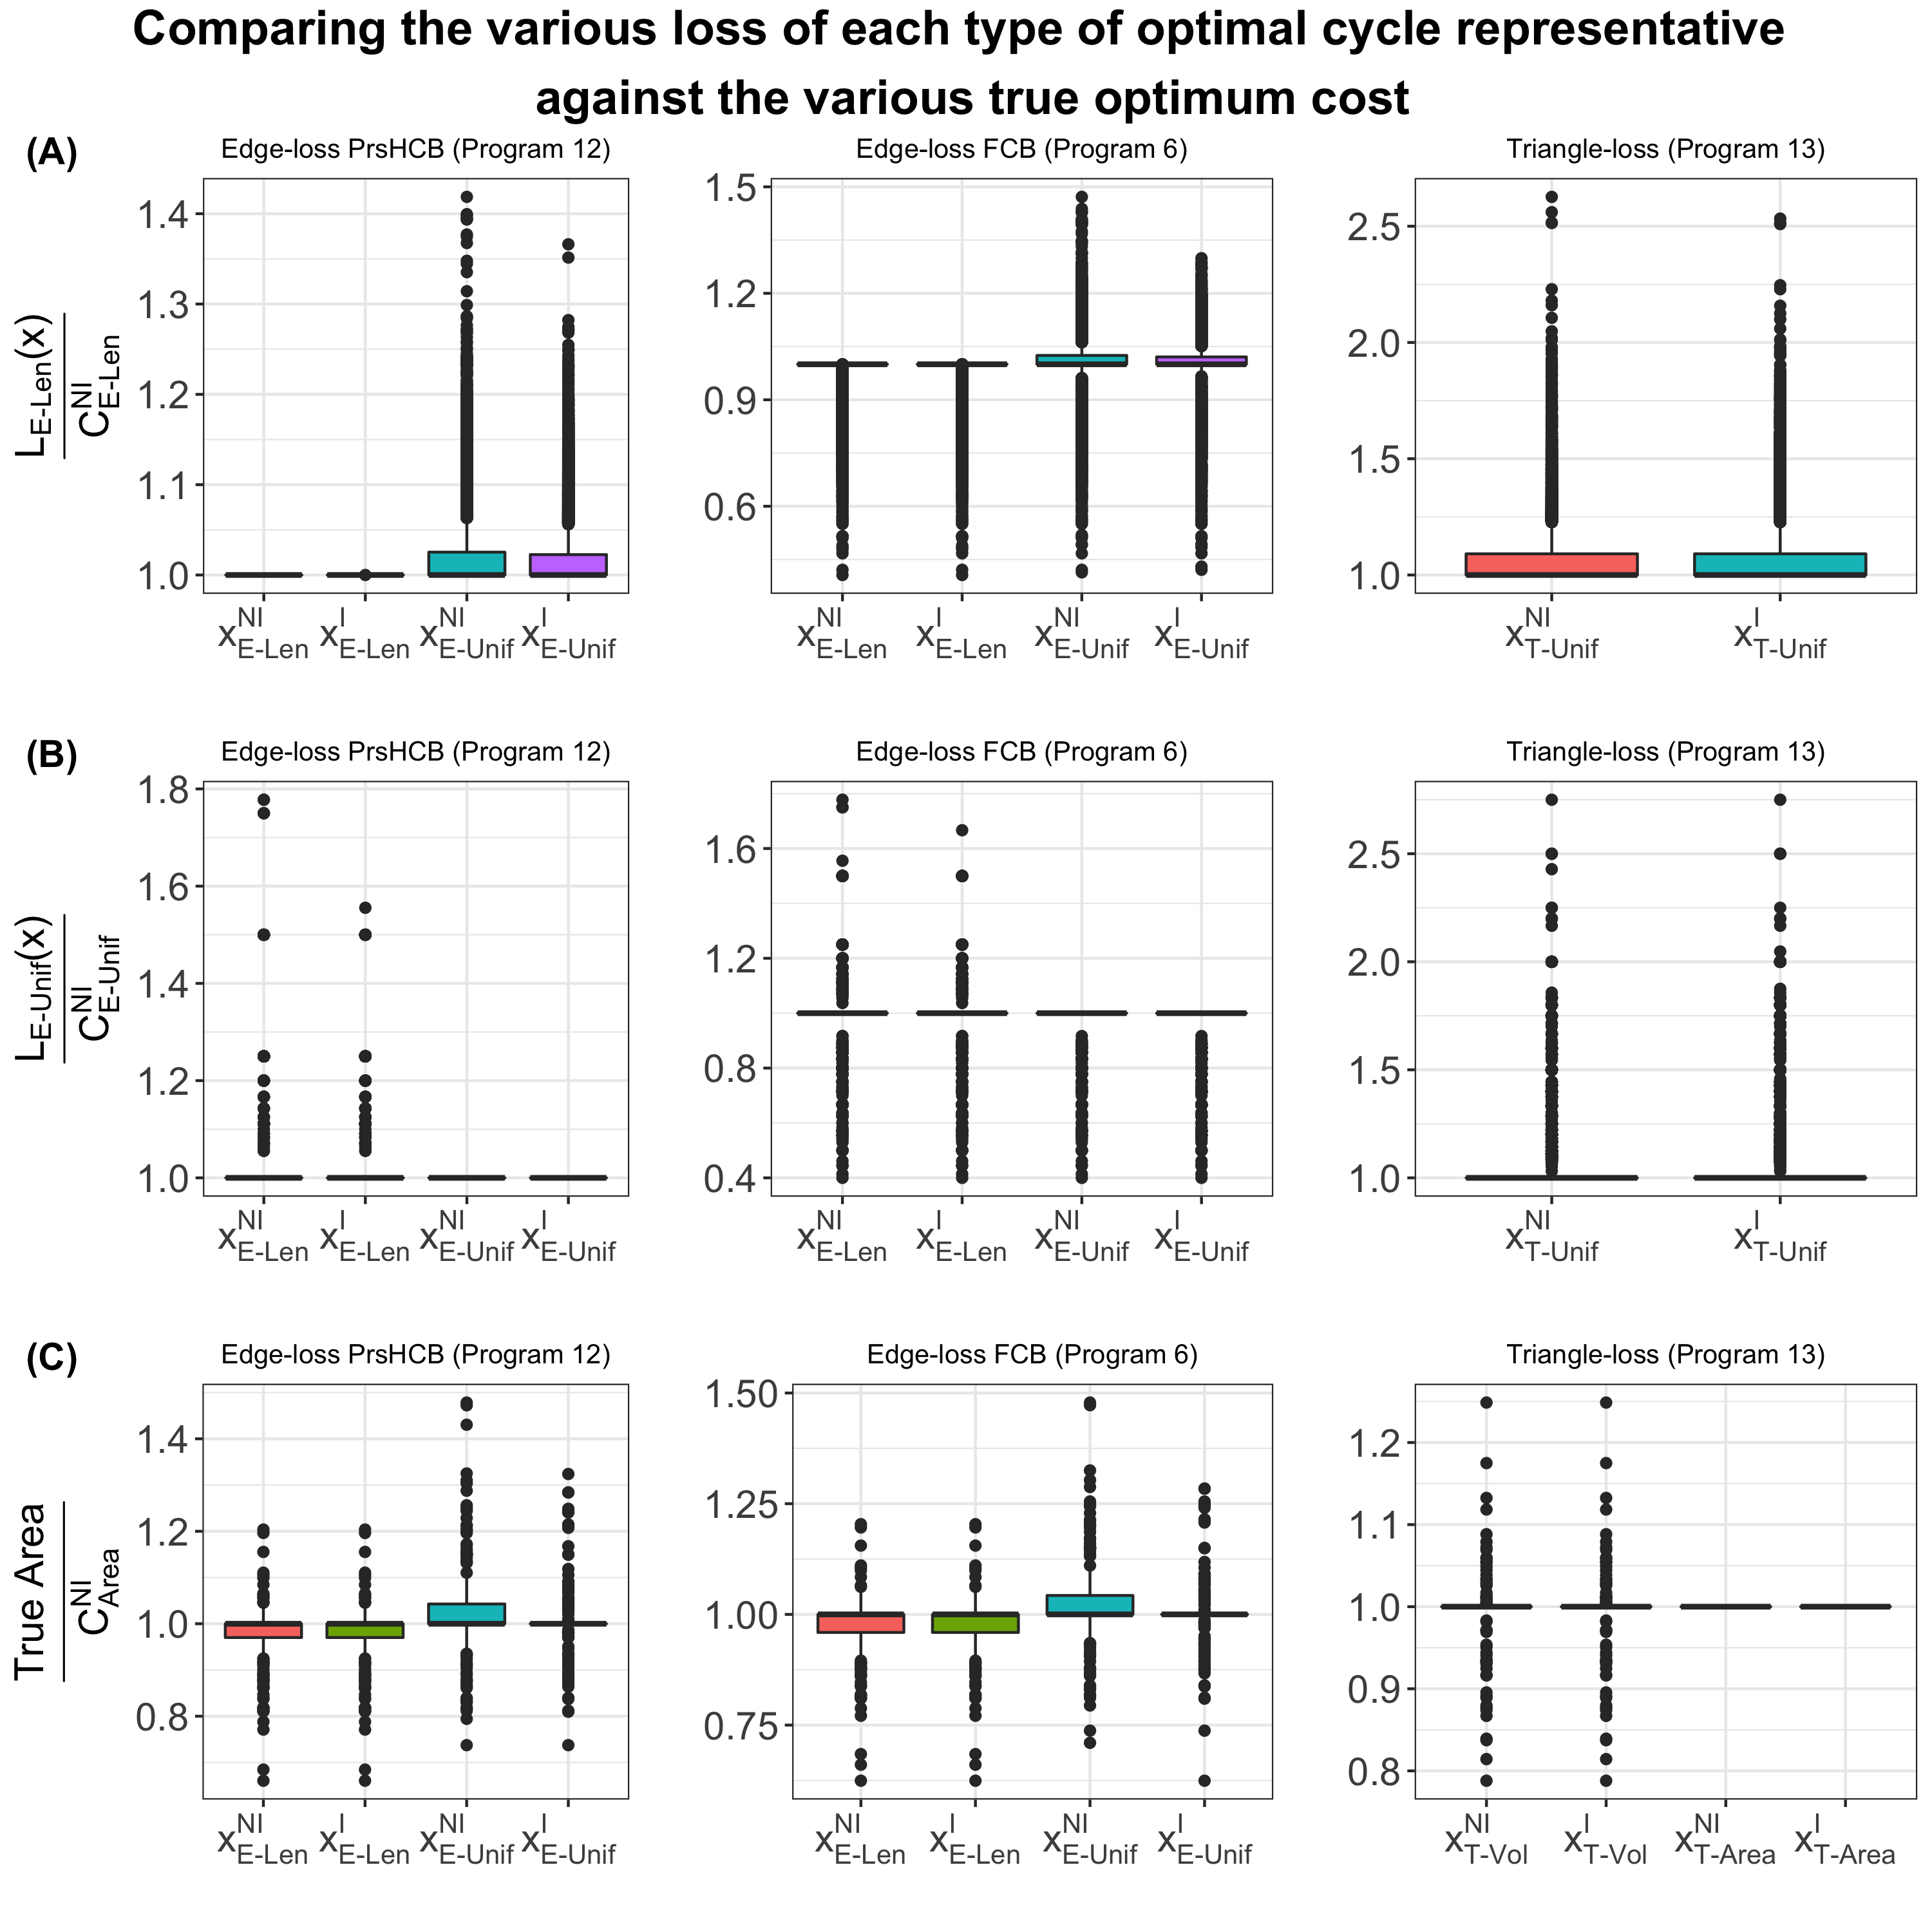
\includegraphics[width=\textwidth]{figures/length_area_edge.png}
%\end{center}
%\caption{Box plot comparing the enclosed area of each type of optimal cycle representative against the optimum area-weighted volume optimal cost. These data aggregate $190$ cycle representatives from $10$ point clouds from a normal distribution with ambient dimension of $2$. True area represents the total area enclosed by the representative, while $C_{Area}\NI$ represents the area of the area-weighted volume optimal cycle minimizing \ref{eq:LP-Area}. We observe that some uniform/length-weighted optimal cycles have an area smaller than that of the area-weighted volume optimal cycle. Refer to Figure \ref{fig:areaExample} to see why this may happen. In addition to $\optimalrep_{Area}\NI = \optimalrep_{Area}\I$ for corresponding cycle representatives in all experiments, so too are $\optimalrep_{Len}\NI = %\optimalrep_{Len}\I$\LZ{Remove, right??}}\label{fig:areacompare}
%\end{figure}

\begin{figure}[h!]
\begin{center}
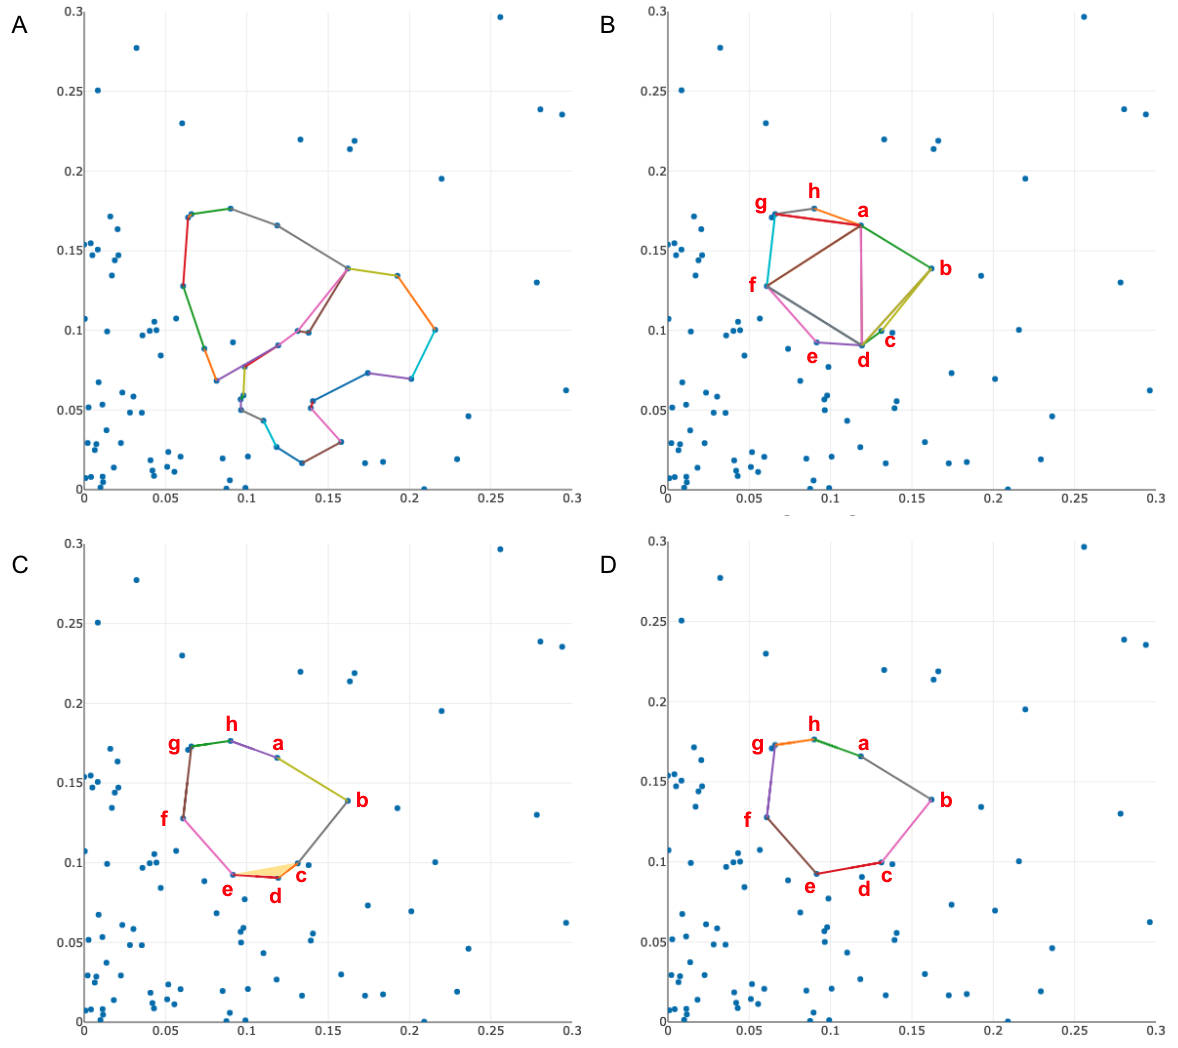
\includegraphics[width=15cm]{figures/areaExample4-2.png}
\end{center}
\caption{An example illustrating when the area enclosed by the triangle-loss area-weighted optimal cycle, solution to \pr \ref{itm:tri_NIA}, can be larger than the area enclosed by the edge-loss length-weighted minimal cycle, solution to \pr \ref{itm:edge_NIL}. \textbf{(A)} is the original cycle of a representative point cloud in $\mathbb{R}^2$ drawn from the normal distribution, \textbf{(B)} is the area-weighted optimal cycle triangulated based on the 2-simplices identified by nonzero entries in the coefficient vector $\volvec$, \textbf{(C)} is the area-weighted minimal cycle, \textbf{(D)} is the length-weighted minimal cycle. The yellow shaded area in \textbf{(C)} marks the difference in enclosed area by the area-weighted and length-weighted minimal cycle representatives. %The area-weighted volume optimal cycle contains the extra 2-simplex $[c,d,e].$
Constraint Equation \eqref{obacond1} specifies that the area-weighted optimal cycle must contain the 2-simplex born at the death time of the cycle. Therefore, this cycle must contain $\{a,d,f\}$ because it was born at the death time, and in fact, it contains both  $\{a,d,f\}$ and  $\{a,b,d\}$. The length-weighted minimal cycle does not have this constraint, and as such, can result in a smaller area. %\LL{Updated 0314}
%To get the length-weighted optimal cycle from the area-weighted volume optimal cycle, we still need to add the $2$-simplex $[c,d,e]$, which will increase the area-weighted volume, but will decrease the enclosed area. \LZ{I rephrased the previous sentence as: The length-weighted optimal cycle adds the $2$-simplex $[c,d,e]$ to the area-weighted volume optimal cycle, which increases the area-weighted volume but decreases the enclosed area....but now I don't think I understand the last part. The length-weighted does not care about the 2-simplices enclosed.}\CT{maybe: Our area-weighted volume optimal cycle differs from the length-weighted optimal cycle by the 2-simplex $[c,d,e]$. Although adding this 2-simplex would decrease the area of the cycle representative, it would increase our measured cost $||W\optimalrep||_1$.} 
}\label{fig:areaExample}
\end{figure}


\begin{figure}[h!]
\begin{center}
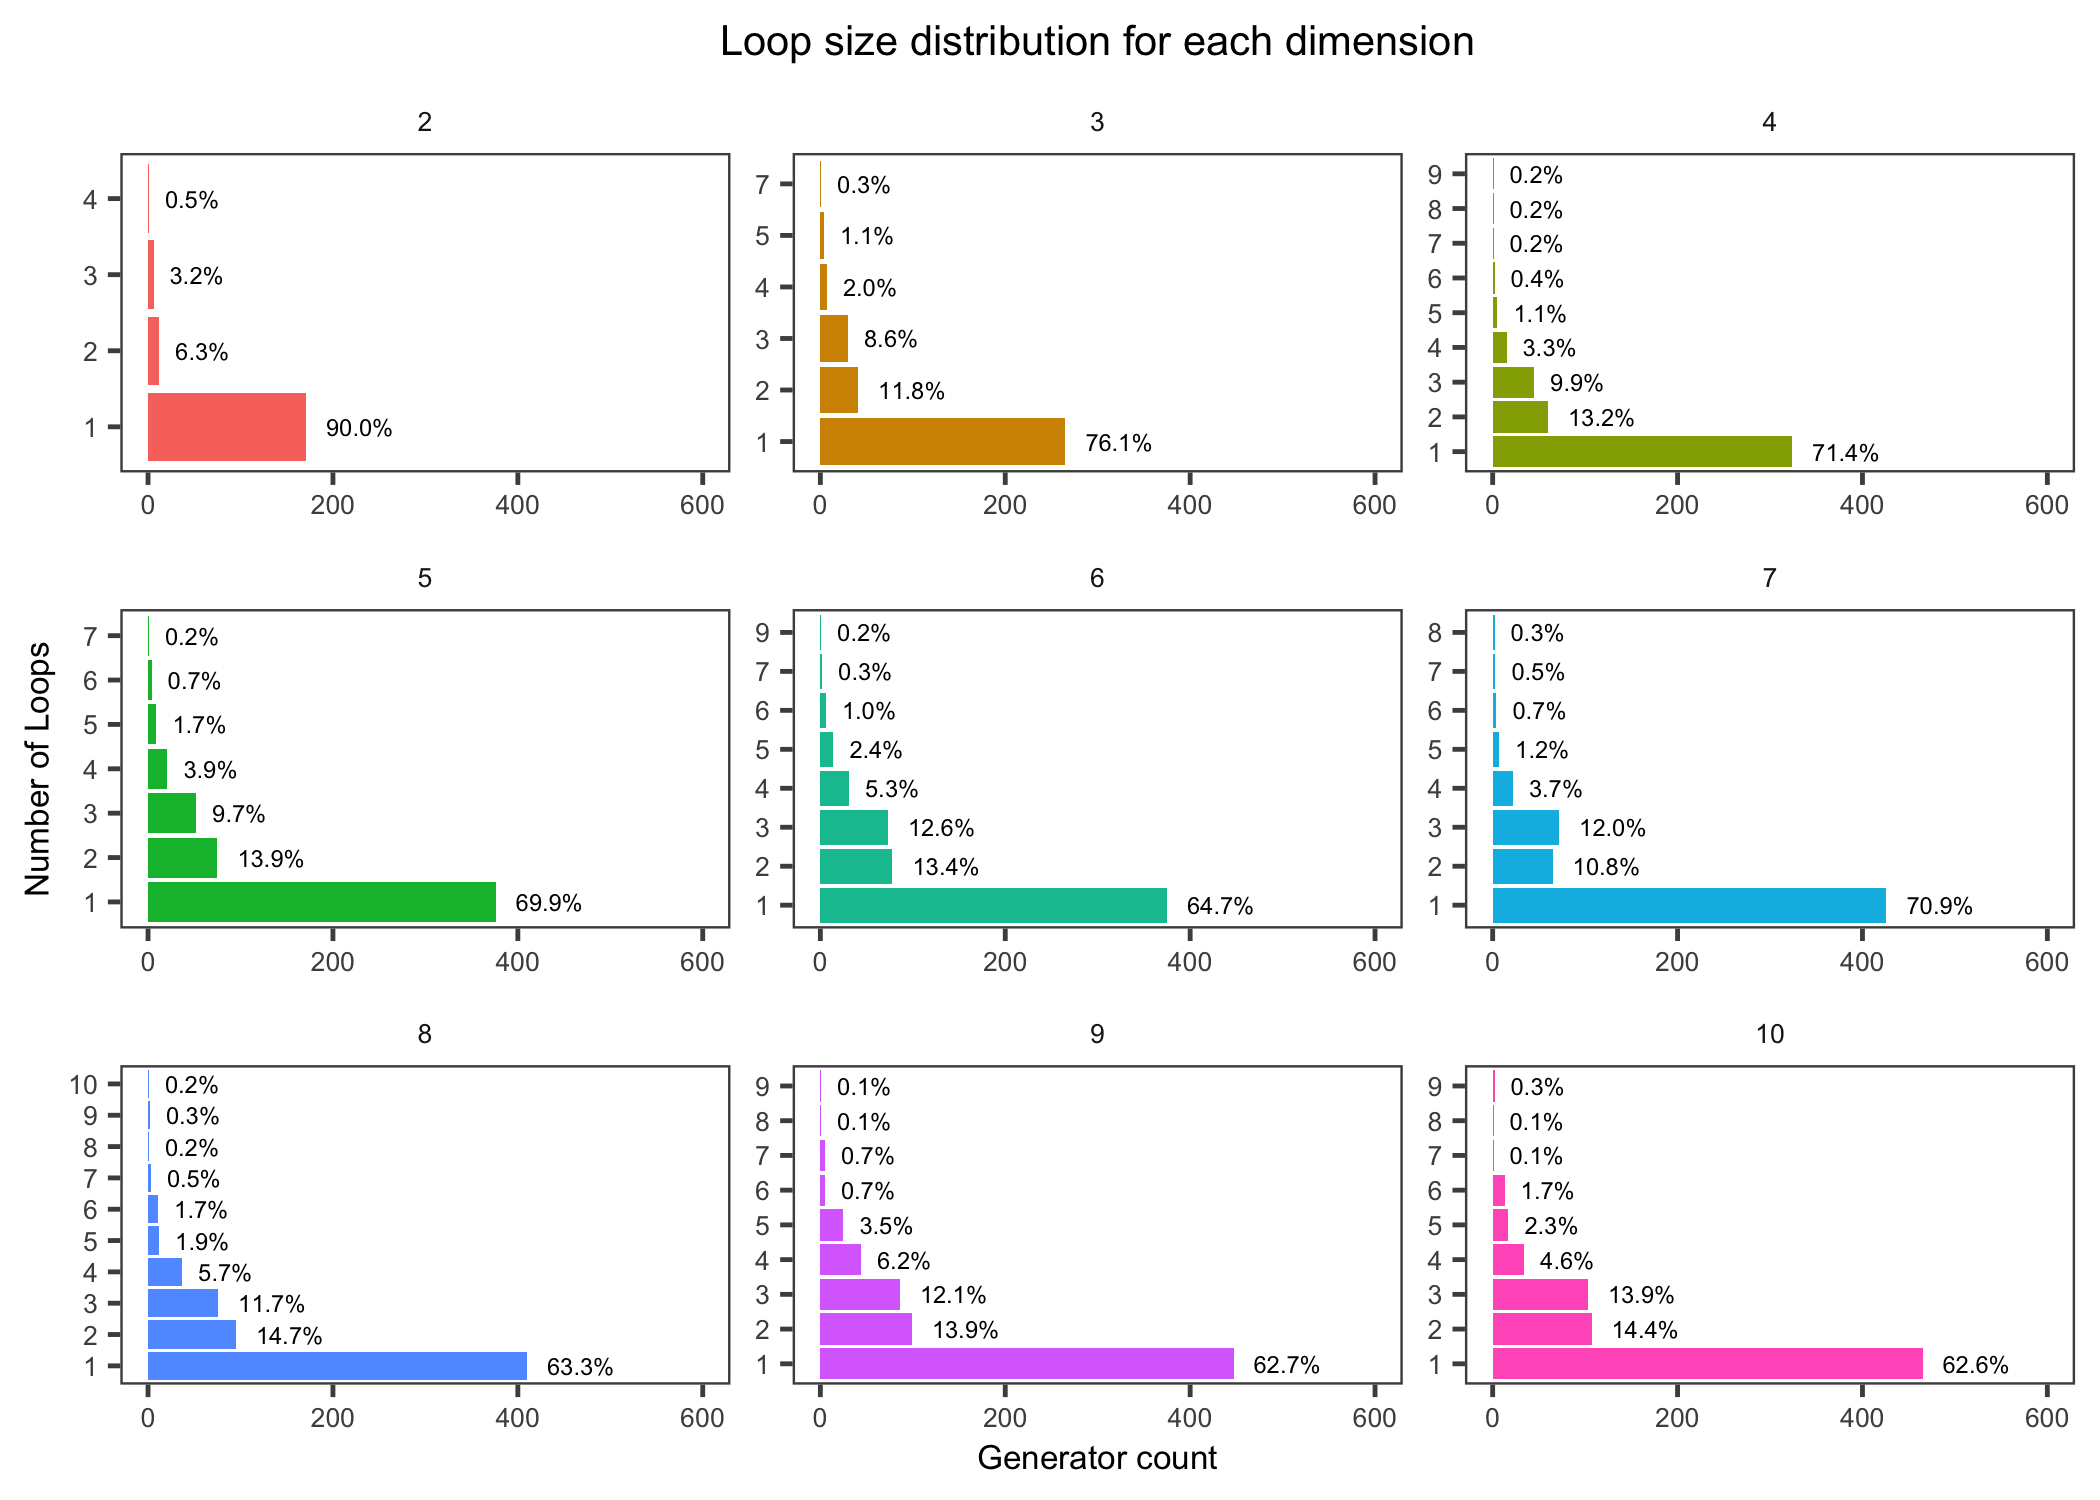
\includegraphics[width=\textwidth]{figures/loopsBreakdown.png}
\end{center}
\caption{%\GHP{First betti number of the support of $\optimalrep$, for various 1-d cycle representatives $\optimalrep$ (equivalently, the nullity of the column submatrix $[\partial_1][:, S]$, where $S = \{i : \optimalrep_i \neq 0\}$ is the support of $\optimalrep$)}\LL{Thanks for this definition, Greg! We added it to the results section 6.8. Should we also keep it here?}  
Number of loops in the original cycle representatives of each dimension (subfigure title) in the $360$ randomly generated distribution data sets. The horizontal axis is the number of representatives and the vertical axis is the number of loops in the original representative. We observe that original cycle representatives can have up to 10 loops in higher dimensions, and in general, it is not uncommon to find an original representative with multiple loops.} \label{fig:loopsbreakdown}
\end{figure} 
% 

% \begin{landscape}
\begin{figure}[h!]
\begin{center}
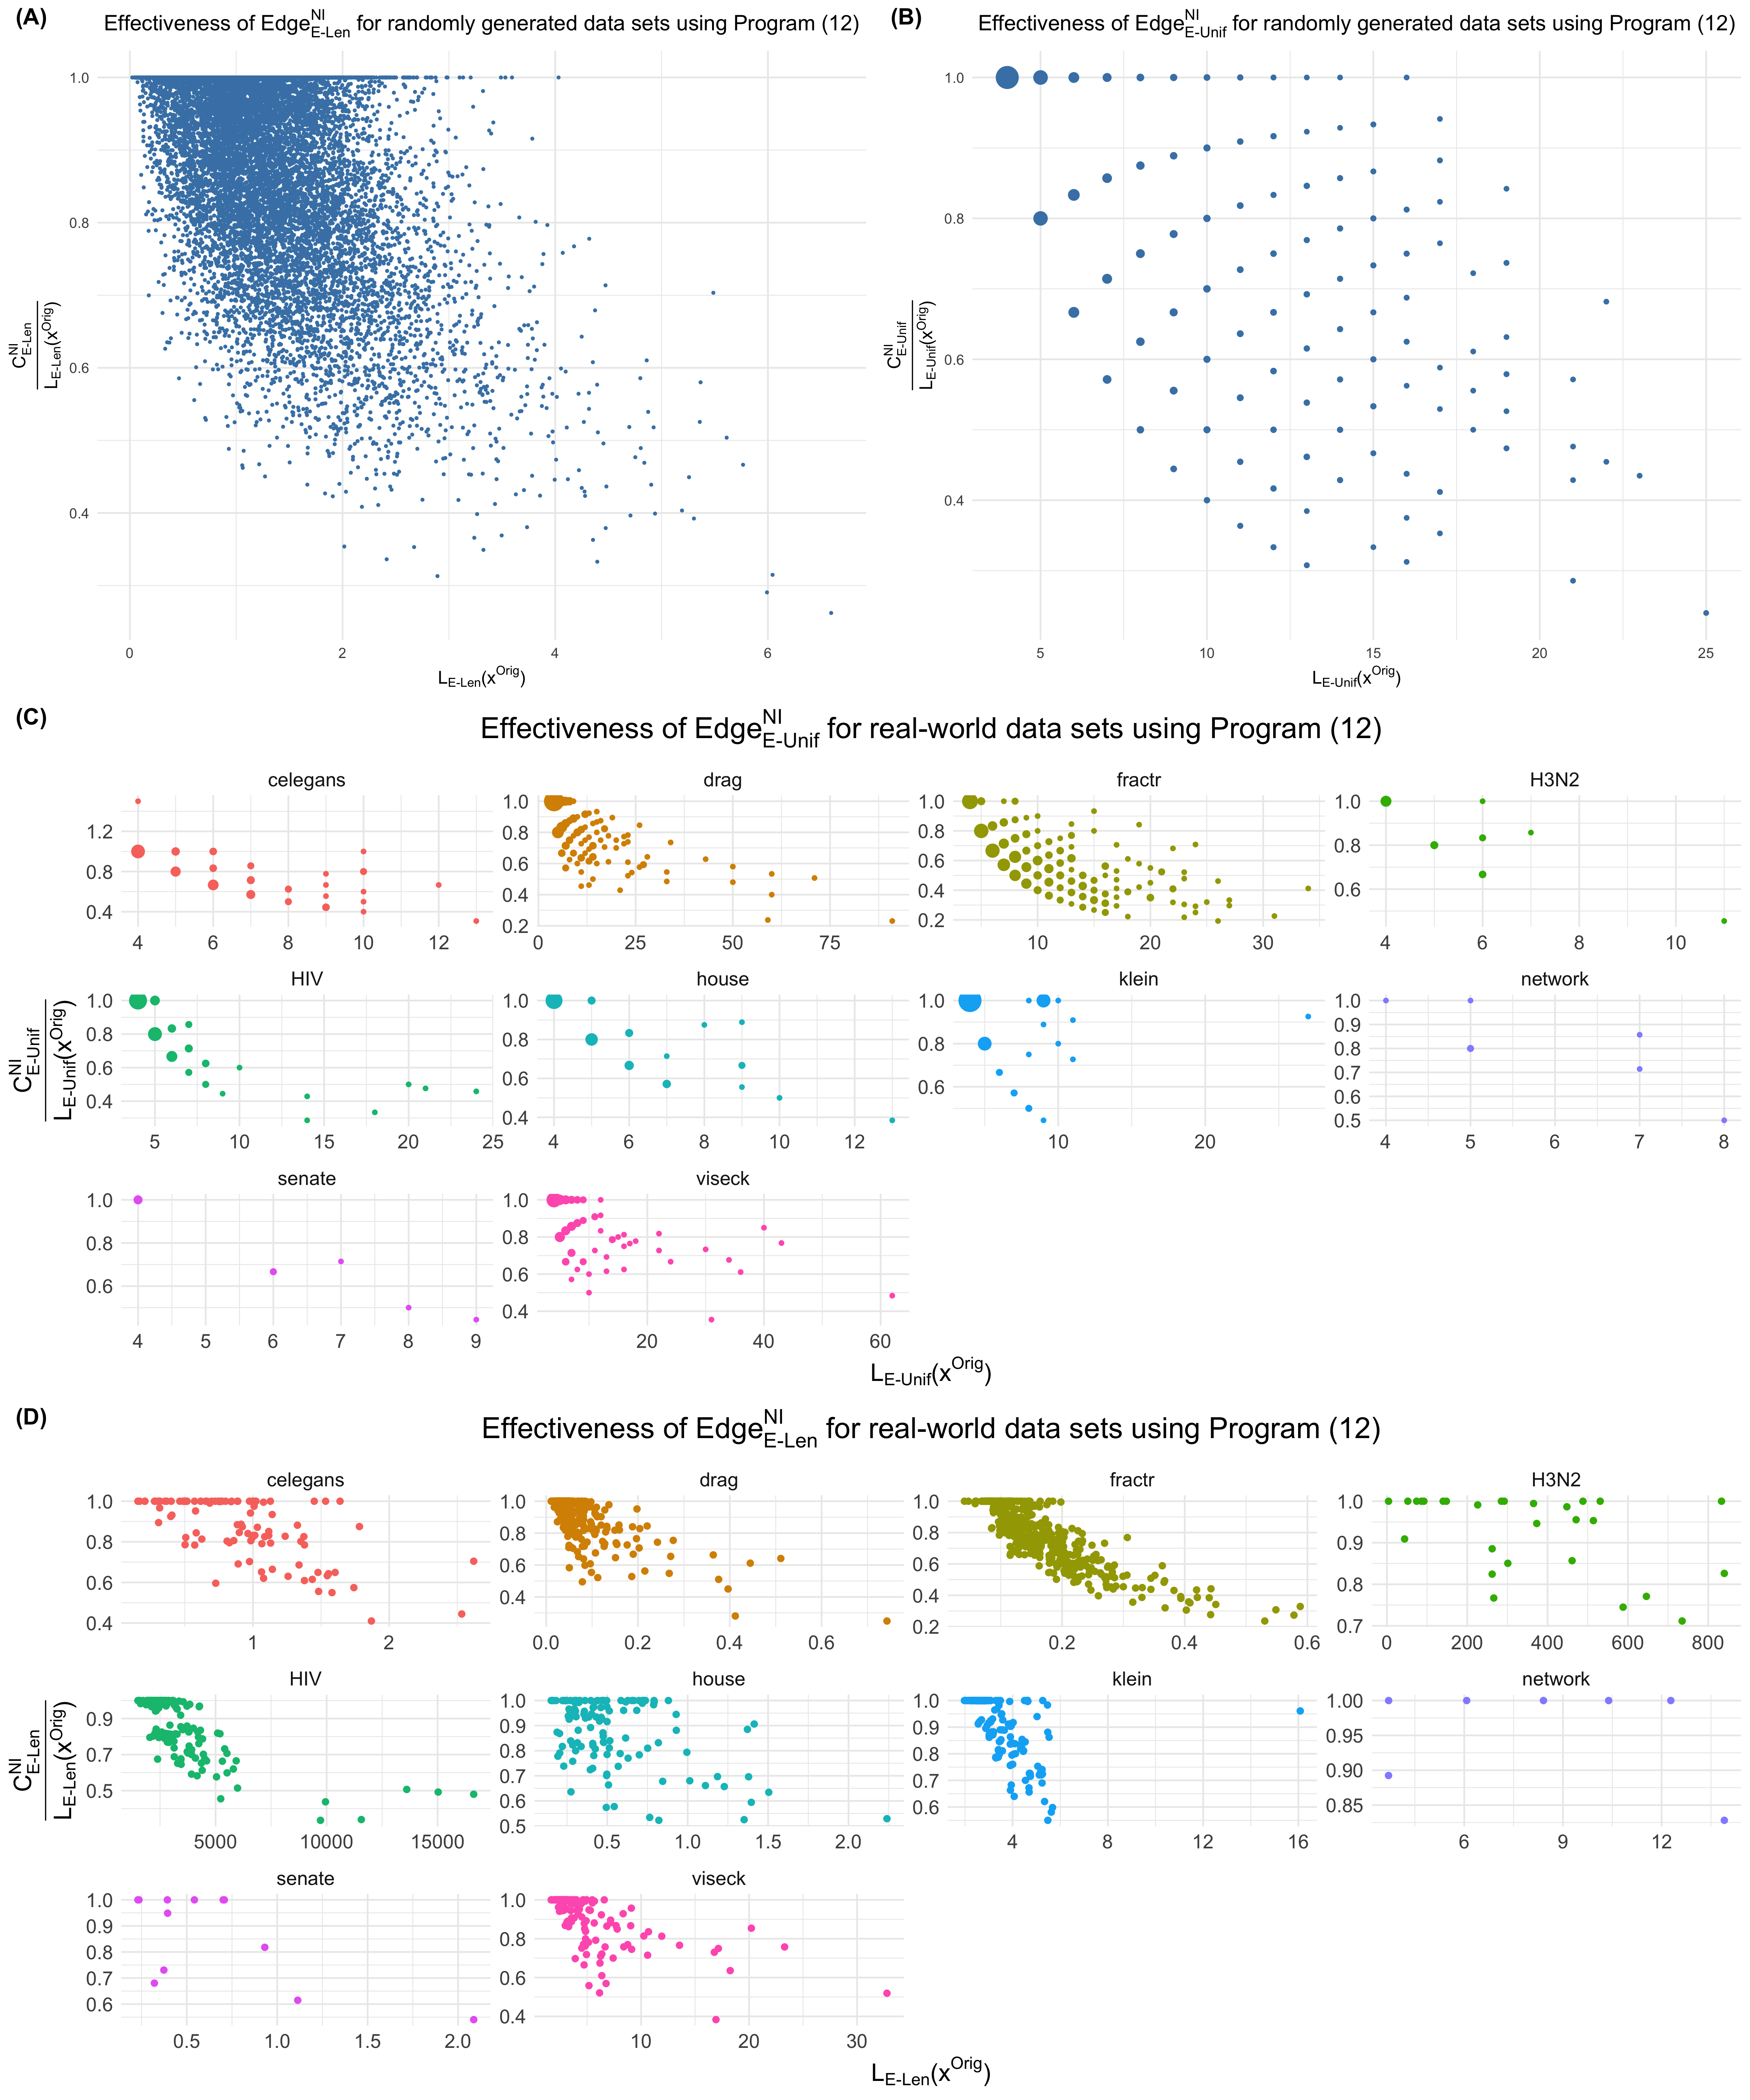
\includegraphics[width=0.95\textwidth]{figures/four_eff_df2.png}% This is a *.eps file
\end{center}
\caption{The effectiveness of length-weighted and uniform-weighted optimization for the randomly generated data sets and real-world data sets in reducing the size of the original cycle representative found by the persistence algorithm. In each subfigure, the horizontal axis is the size of the original representative and the vertical axis is the ratio between the size of the optimal representative and the size of the original representative. The uniform-weighted graphs appear more sparse because reductions in the cost $L_{T\text{-}Unif}(\originalrep)$ can only come in multiples of the reciprocal of the original length. The node size in the uniform-weighed graphs corresponds to the number of overlapping points. %\LL{updated! 0314}
}\label{fig:effectivenessall}
\end{figure}
% \end{landscape}

% \begin{figure}[h!]
% \begin{center}
% 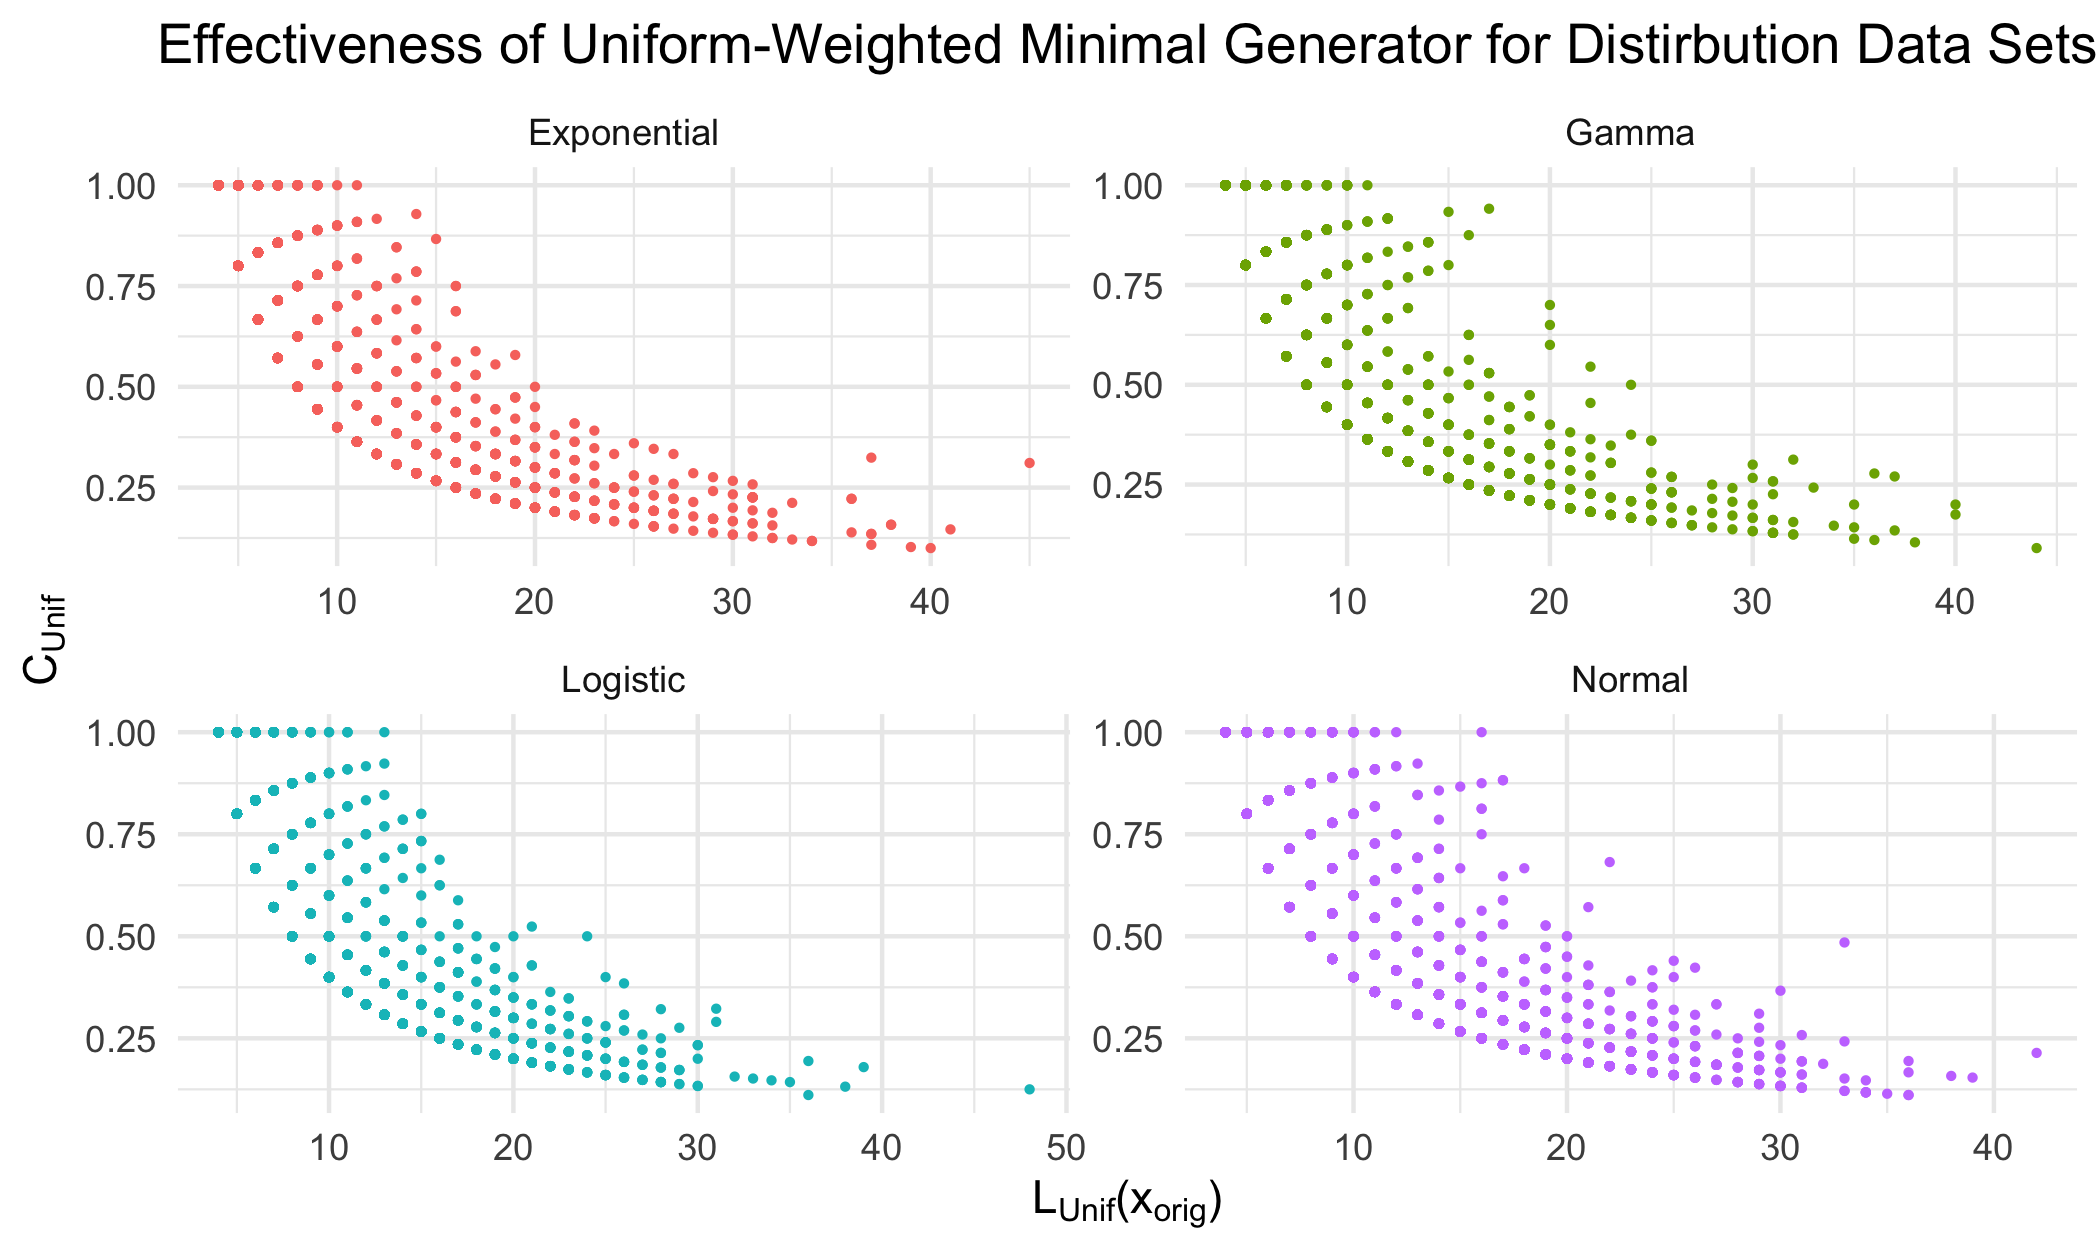
\includegraphics[width=1\textwidth]{figures/edge_eff_dist.png}% This is a *.eps file
% \end{center}
% \caption{Effectiveness of Uniform-Weighted Minimal Generator for Distribution Data Sets}\label{fig:edge_eff_dist}
% \end{figure}

% \begin{figure}[h!]
% \begin{center}
% 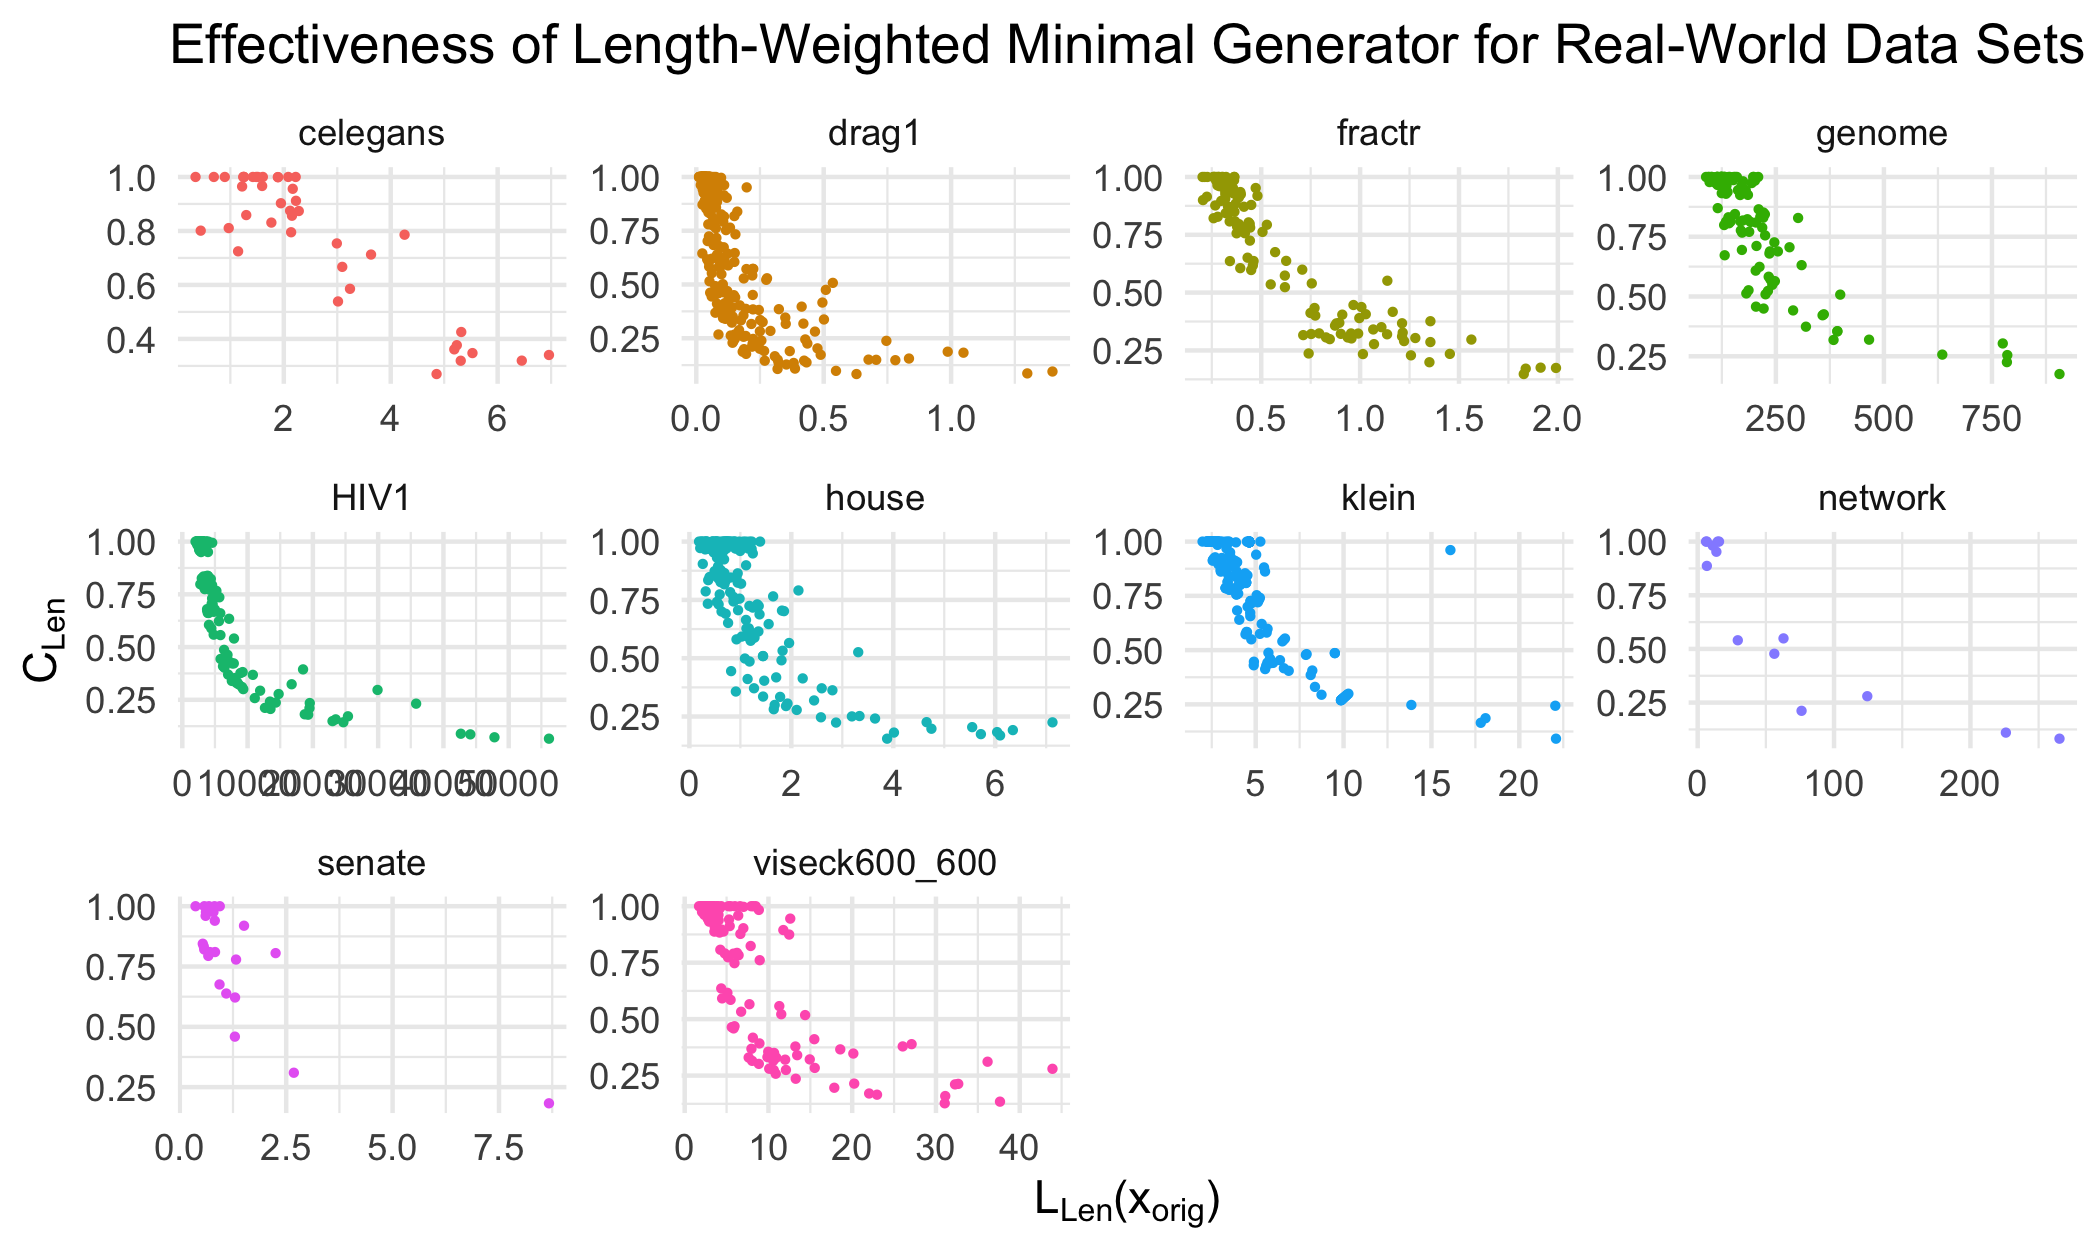
\includegraphics[width=1\textwidth]{figures/length_eff_df.png}% This is a *.eps file
% \end{center}
% \caption{Effectiveness of Length-Weighted Minimal Generator for Real-World Data Sets}\label{fig:length_eff_df}
% \end{figure}
% \begin{figure}[h!]
% \begin{center}
% 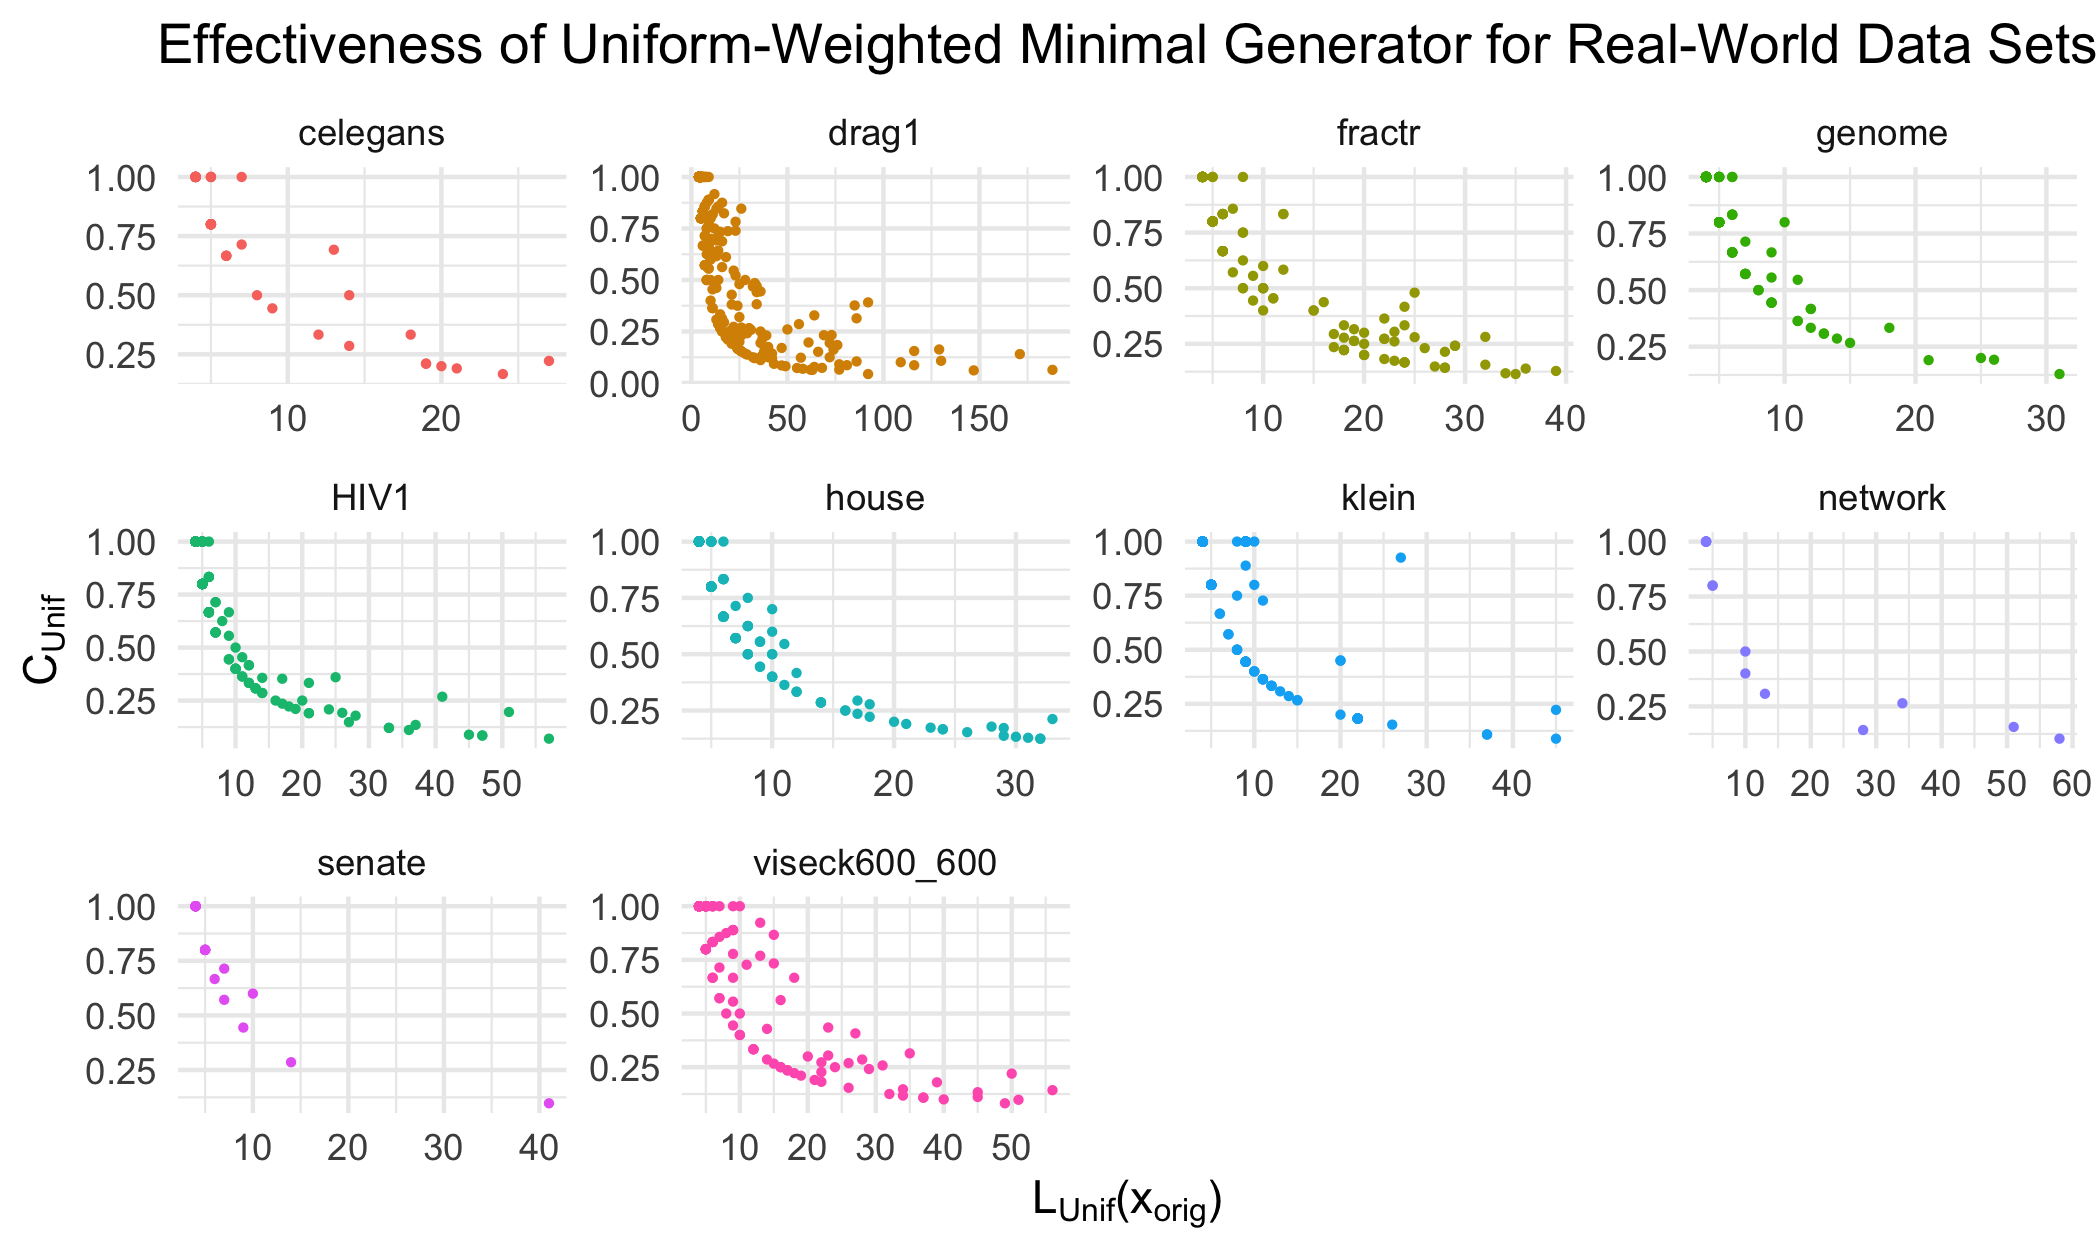
\includegraphics[width=1\textwidth]{figures/edge_eff_df.png}% This is a *.eps file
% \end{center}
% \caption{Effectiveness of Uniform-Weighted Minimal Generator for Real-World Data Sets}\label{fig:edge_eff_df}
% \end{figure}

\begin{figure}[h!]
\begin{center}
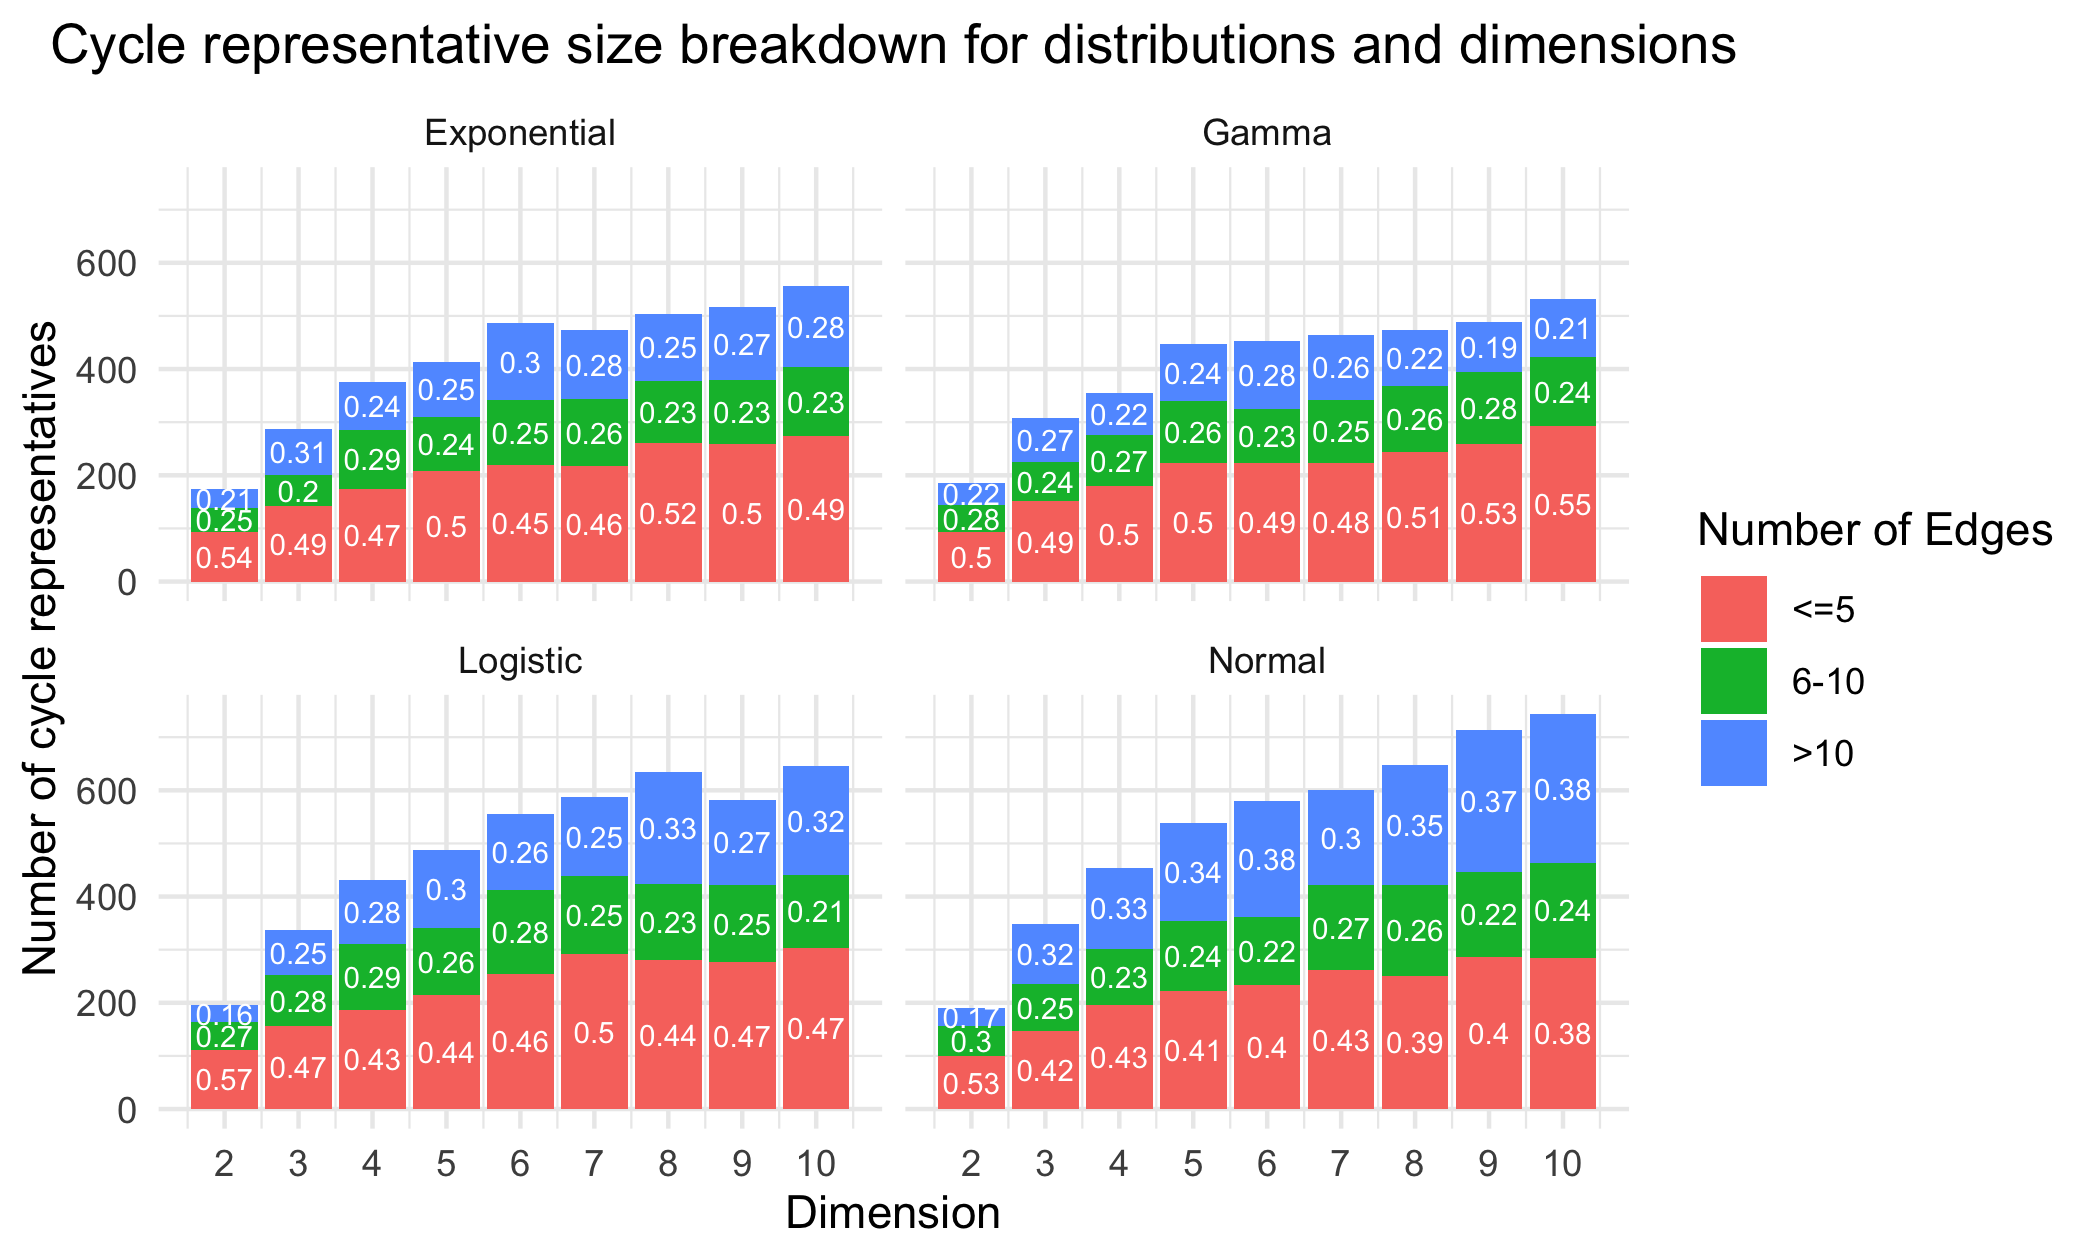
\includegraphics[width=1\textwidth]{figures/generator_breakdown.png}% This is a *.eps file
\end{center}
\caption{The number of original cycle representatives and the number of edges within each original representative for data described in \se \ref{sec: randompointclouds}. These plots aggregate all cycle representatives for each dimension of a particular distribution. The horizontal axis for each subplot is the dimension of the data set, and the vertical axis is the number of cycle representatives found in each dimension. In general, we see there are more cycle representatives in higher dimensional data sets. Each bar is partitioned by the number of edges of the representative. We observe that as dimension increases, there tend to be more cycle representatives with more edges. %\LL{updated 0314}
}\label{fig:gen_num_breakdown}
\end{figure}


% % \begin{figure}[h!]
% \begin{center}
% 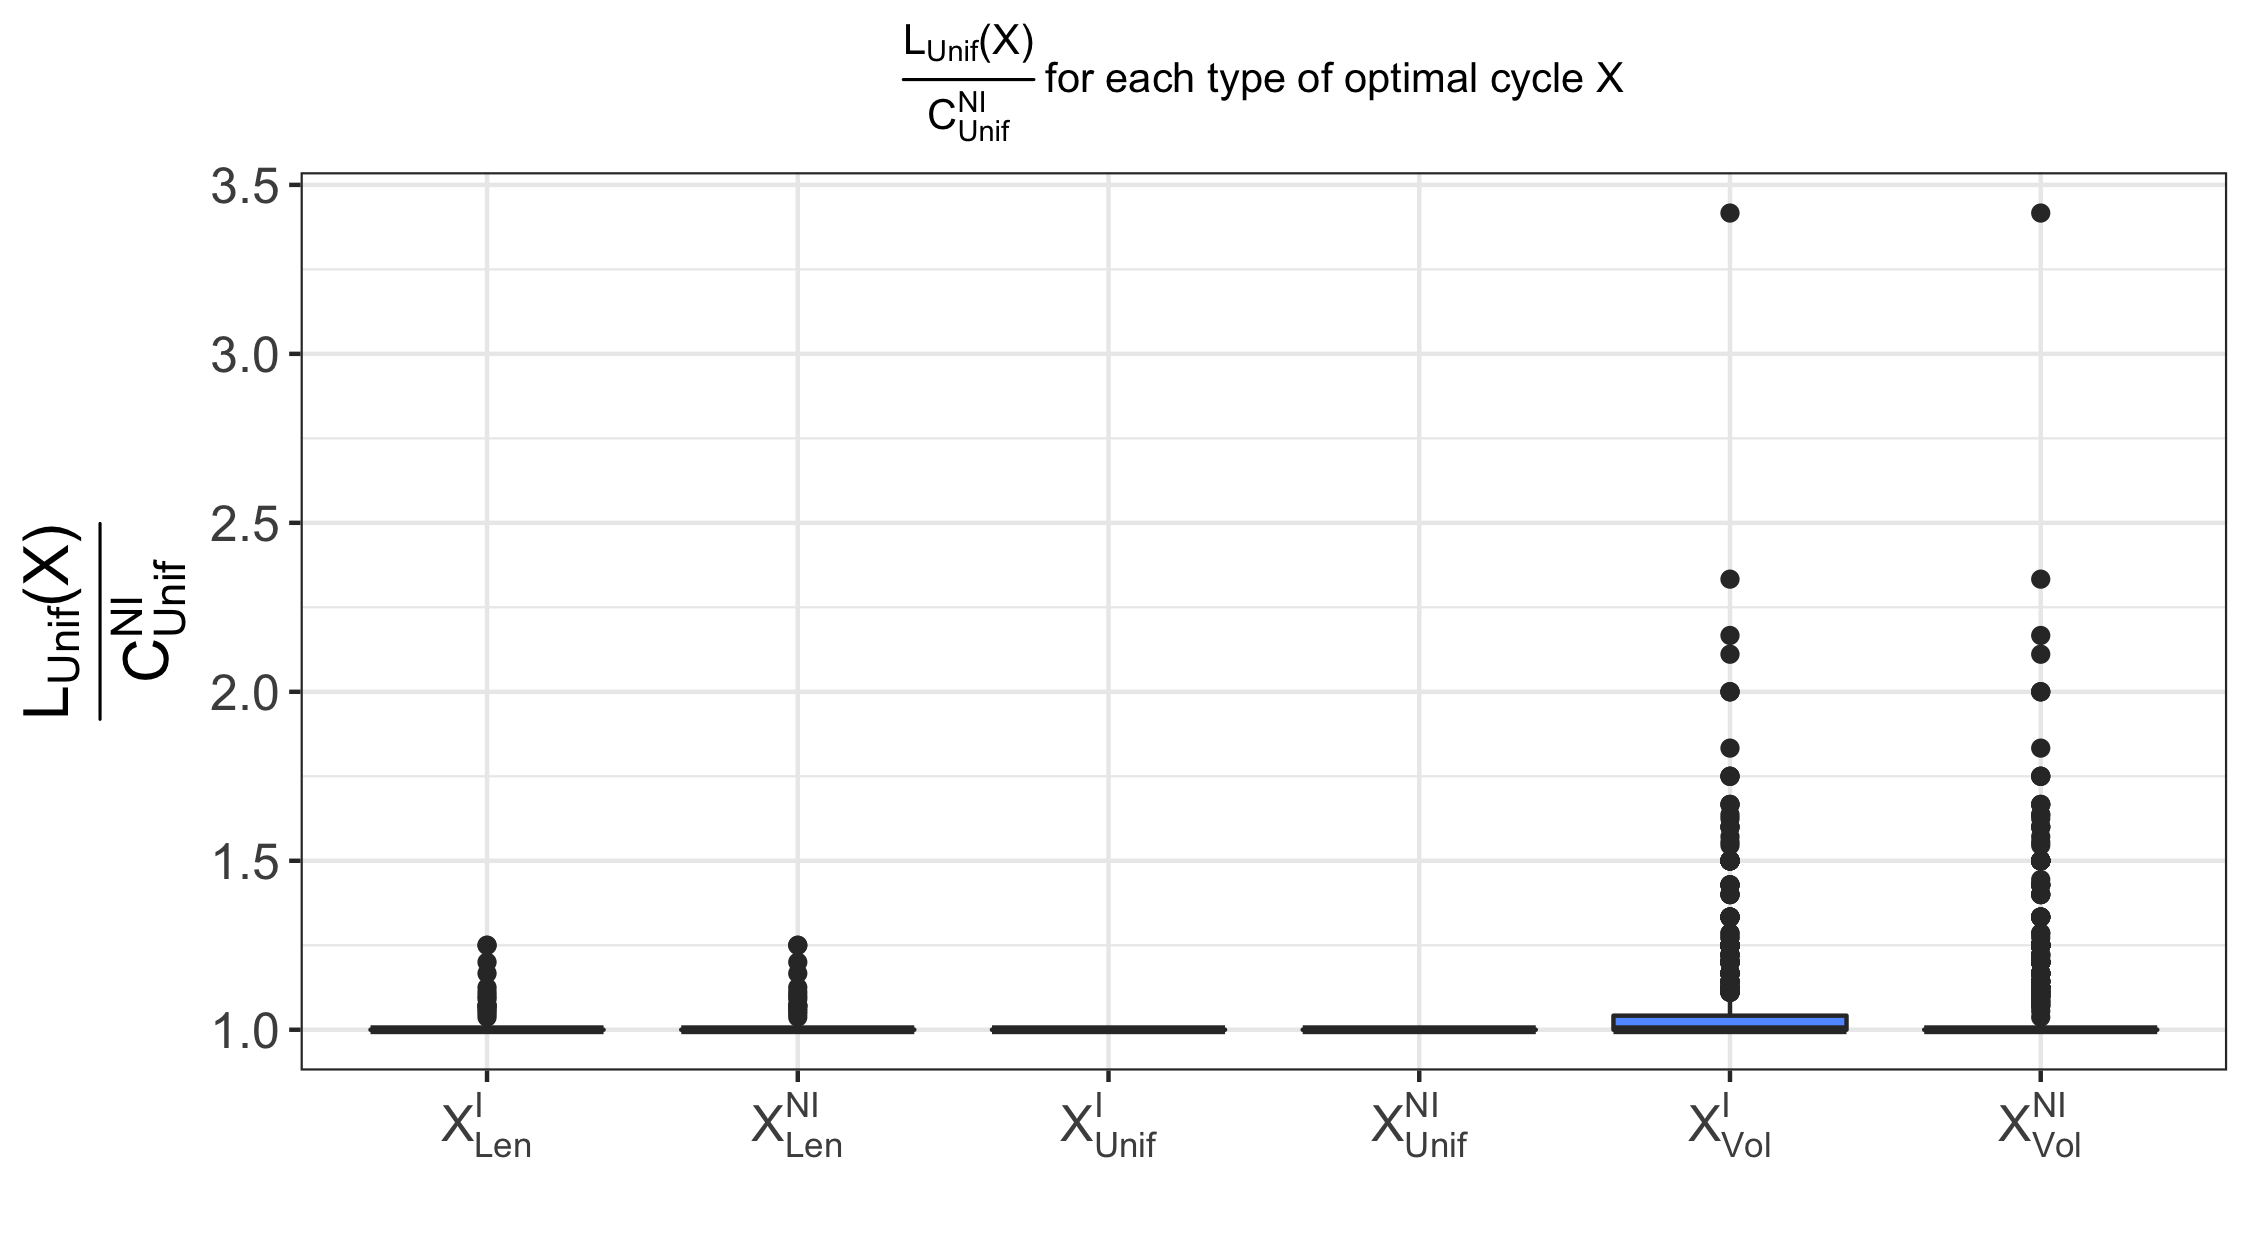
\includegraphics[width=\textwidth]{figures/edge_compare.png}
% \end{center}
% \caption{Box plots comparing the uniform-weighted loss of each type of optimal cycles against the uniform-weighted optimum cost. The $x$-axis is the type of optimal cycle and the $y$-axis is the ratio between the uniform-weighted cost of each type of optimal cycle and the actual uniform-weighted cost of the uniform-weighted minimal cycle (i.e. the number of edges in the cycle) without requiring integral solutions. We expect the middle two columns to be 1 as the optimums obtained whether requiring integral solutions or not are the same in all our experiments.}\label{fig:edgecompare}
% \end{figure}




% \begin{landscape}

\begin{table}[!h]
\caption{distmat}
    {\footnotesize{
    % \begin{tabular}{ |>{\centering\arraybackslash}m{3cm} | {\centering\arraybackslash}m{1.5cm} |  >{\centering\arraybackslash}m{1.8cm} | {\centering\arraybackslash}m{1.5cm} |  >{\centering\arraybackslash}m{2cm}|   >{\centering\arraybackslash}m{2cm}| >{\centering\arraybackslash}m{2cm} | >{\centering\arraybackslash}m{2cm}|  >{\centering\arraybackslash}m{2cm}| >{\centering\arraybackslash}m{1.3cm}| >{\centering\arraybackslash}m{2cm} | >{\centering\arraybackslash}m{2cm} |}
    
    \begin{tabular}{ |>{\centering}m{11em} *{11}{>{\centering\arraybackslash}m{4.5em} }|}
 \hline
  & \textbf{Klein} & \textbf{Vicsek}  & \textbf{C.elegans} & \textbf{HIV} & \textbf{Genome}  & \textbf{fractal R} & \textbf{network} & \textbf{house} & \textbf{senate} & \textbf{drag} & \textbf{H3N2}\\[0.5ex] 
 \hline 
 \hline
 \textbf{Ambient dimension} & 3 & 3 & 202 &  673 & 688 &  259 & 300 & 261 & 60 & 3 &  1,173\\   
 \textbf{\# points}   & 400 &  300  &  297 &   1088 &  1397  & 512 & 379 & 445  & 103 & 1,000 & 2,722\\ 
 \textbf{\# representatives}&   & 124  &  107 &174   &     & 438 & 7  & 126  & 12 &  & 28 \\  
 \textbf{$T$ persistence}   &   & 6.81 & 5.14 &728.51&     & 143.07 & 12.18  &  9.62 & 0.10 &  & 71,081.77  \\ 
 [0.5ex] 
\hline
\multicolumn{5}{c}{\textbf{\qquad Edge-loss persistent homological cycle representatives (\pr \eqref{eq:edgelossgeneral})}} &&&&&& \\
\hline
%  \textbf{Memory (GiB)}    & 5.56 & 3.05 & 199.52 & 181.27  & 7.71 & 72.17 & 7.16 & 0.15& 416.38\\ \hline        
 \textbf{$T\I_{E\text{-}Len}$ optimization} &   & 8.2 &  19.64&466.85  &     & 150.46 & 0.17 & 63.93  & 0.31 &  & 4,732.59	\\ 
 \textbf{$T\NI_{E\text{-}Len}$ optimization} &   & 6.61 &16.07  &403.63 &     & 86.95 & 0.13 & 48.65  & 0.22 &  & 4,540.55 \\ 
 \textbf{$T\I_{E\text{-}Unif}$ optimization} &   & 9.09 & 19.22 & 473.82 &     & 119.94 & 0.23 &  63.34 & 0.33 &  & 4,714.90	\\ 
  \textbf{$T\NI_{E\text{-}Unif}$ optimization} &   & 5.55 & 15.63 & 404.95 &     & 83.40 & 0.12 & 48.88  & 0.22 &  & 4,547.37 \\
  [0.5ex] 
\hline
\multicolumn{5}{c}{\textbf{Edge-loss filtered homological cycle represnetatives (\pr \eqref{eq:escolarargmin})}} &&&&&& \\
\hline
%  \textbf{Memory (GiB)}    & 5.56 & 3.05 & 199.52 & 181.27  & 7.71 & 72.17 & 7.16 & 0.15& 416.38\\ \hline        
 \textbf{$T\I_{E\text{-}Len}$ optimization} &   &8.64  &20.41  & 468.22 &     &  155.08&  0.17 &  62.2  & 0.30 &  & 2,999.24	\\ 
 \textbf{$T\NI_{E\text{-}Len}$ optimization} &   & 5.51 &16.15  & 403.74 &     & 88.66 &0.13  &  48.24 & 0.22 &  & 2,829.12	\\ 
 \textbf{$T\I_{E\text{-}Unif}$ optimization} &   & 8.32 &19.76  & 476.84  &     &  142.4&  0.24  & 61.82  & 0.31 &  & 2,937.16	\\ 
  \textbf{$T\NI_{E\text{-}Unif}$ optimization} &   & 5.63 & 16.23 & 406.97 &     & 87.59 &  0.12 & 48.11  &0.22  &  & 2,833.06	 \\
  [0.5ex] 
\hline
\multicolumn{5}{c}{\textbf{Triangle-loss persistent homological cycle representatives (\pr \eqref{eq:trianglelossgeneral})\qquad}} &&&&&& \\
\hline
 \textbf{$T\I_{T\text{-}Unif}$ optimization} & & 23.07  &783.06  & 63,227.14 &  &  10,187.41   & 2.71 & 221.07  & 0.26  &  & 39,140.67 \\ 
 \textbf{$T\NI_{T\text{-}Unif}$ optimization} & & 18.81 & 610.20 &60,459.49 &  &   8,441.76  & 2.08 & 170.95  & 0.23  &  & 36,401.50  \\ 
 \textbf{$T$ build all}  & & 0.88  &  &  &  & 45.28 & 0.05 &  4.85 & 0.03  &  & \\ 
\textbf{Total $T$ build part}  & & 3.06  &24.21 & 860.91 &  & 193.99 & 0.26 & 31.37  & 0.03  &  & 922.50 \\ \hline 
\end{tabular}
}%\LL{Updated 03/14}
}
\label{tab:realworldata}
\end{table}
% \end{landscape}
% \begin{table}[!h]
%     \centering
%     \begin{tabular}{ |c || c |c |c |c | c| c|c|c|c|c|}
%  \hline
%  & Klein & Vicsek600  & eleg & HIV & Genome  & fractal R & network & house & senate & drag\\[0.5ex] 
%  \hline 
%  Ambient dimension & 3 & 3    & 202 &  673 & 688 &  259 & 300 & 261 & 60 & 3\\\hline  
%  \# points &  400 &  300  &  297 &   1088 &  1397  & 512 & 379 & 445  & 103 & 1000\\\hline  
%  $T$ persistence &   95.56  & 8.74  & 3.39 & 552.80 &  1079.96  & 62.99 & 31.73 & 7.79 & 0.12 & 1037.70 \\ \hline
%  Memory (GiB) &   50.77  & 5.56 & 3.05 & 199.52 & 181.27  & 7.71 & 72.17 & 7.16 & 0.15& 416.38\\ \hline        
%  \# generators & 257 & 124  &42& 199& 117& 126&  13 & 133 & 19& 311\\ \hline
%  $T\I_{Len}$ optimization &2,253.14   & 358.72    & 47.75 &  8,140.87  & 48,109.66  & 2,700.03 &   17.05 & 347.09 &    1.18 & 8,305.27 \\ \hline
%  $T\NI_{Len}$ optimization& 2,163.14  & 308.56  & 26.53 & 5,101.00 &23,264.60  &2,000.97  &  11.43   &138.36   &  0.91  &7,280.97 \\ \hline 
%  $T\I_{Unif}$ optimization &2,323.93&   362.77&    47.62  &8,700.25& 46,754.56  &2,830.24  &  18.59   &311.09&     1.16&  8,339.93 \\ \hline
%   $T\NI_{Unif}$ optimization &2,212.52   &309.72  &  26.55  &5,004.96& 23,323.30&  2,222.38 &   11.54  & 138.73 &    0.90 &  7,305.24 \\ 
%  \hline
%  $T\I_{Vol}$ optimization &  & 140.04  &  223.97 &  16,691.24  & 16,328.65 &  6,849.59 &    7.52  & 204.31 &   0.36  &  443.89\\ \hline
%  $T\NI_{Vol}$ optimization&   & 130.95 & 169.08 & 14,547.61 & 14570.72 & 5,939.54&  8.01  & 172.66  &  0.30 & 398.79\\ \hline 
%  T build all triangles &   & 14.86 & 9.76 &  & - & 47.8 & 11.76  &   &  0.04 & 172.60\\ \hline 
% Total deleting time &   & 0.01 & 0.05 &  & &  & 0.00  &    &  0.00 & \\ \hline 
% Total build-part time &   &  &   8.28 &  475.37 & 437.75 & 268.57 &  1.06 & 28.42 &    & 242.14\\ \hline 

% \end{tabular}
% \caption{External Data Sets (Time measured in seconds)}
% \label{tab:data}
% \end{table}
% \end{center}




\begin{table}[!h]
\caption{\caption{Summary of the experimental results of the data sets from \cite{roadmap2017} as described in \se \ref{sec: realworlddata}. The rows include the ambient dimension, number of points, the number of cycle representatives in $\Homologies_1$, and the time (measured in seconds) it took to compute persistent homology for each data set. We also include the computation time taken to optimize the set of cycle representatives under six different optimization problems, and computation time of two different implementation choices for the triangle-loss optimal cycles: building the full $\partial_2$ boundary matrix once and extracting the part needed, or constructing part of the $\partial_2$ boundary matrix for each cycle representative. In this table, $T$ stands for computation time measured in seconds with subscripts indicating the type of the optimal cycle and superscripts indicating whether the program was solved using linear programming (NI) or integer programming (I). The time taken to construct the input to the optimization problem is included in the optimization time for edge-loss minimal cycle representatives, but is excluded and separately listed in the last two rows for the triangle-loss minimal cycle representatives. For triangle-loss cycles, we were able to compute $115$ out of the $117$ cycle representatives for the \textbf{Genome} data set and $52$ out of $57$ cycle representatives for the \textbf{H3N2} data set due to memory constraints. The numbers in the parenthesis represent the other optimization statistics corresponding to the triangle-loss optimal cycles we were actually able to compute. The last two rows compare two ways of building the input $\partial_2[:,\hat {\mathcal{F}}_{2}]$ matrix to the triangle-loss optimal cycle program. The penultimate row records the time of building the entire $\partial_{2}$ matrix once and then extracting columns born in the interval $\closedinterval$ for each representative. The last row records the total time to iteratively build the part of the boundary matrix $\partial_2[:,\hat {\mathcal{F}}_{2}]$ for each cycle representative.}
}
    {\footnotesize{
    % \begin{tabular}{ |>{\centering\arraybackslash}m{3cm} | {\centering\arraybackslash}m{1.5cm} |  >{\centering\arraybackslash}m{1.8cm} | {\centering\arraybackslash}m{1.5cm} |  >{\centering\arraybackslash}m{2cm}|   >{\centering\arraybackslash}m{2cm}| >{\centering\arraybackslash}m{2cm} | >{\centering\arraybackslash}m{2cm}|  >{\centering\arraybackslash}m{2cm}| >{\centering\arraybackslash}m{1.3cm}| >{\centering\arraybackslash}m{2cm} | >{\centering\arraybackslash}m{2cm} |}
    
    \begin{tabular}{ |>{\centering}m{11em} *{11}{>{\centering\arraybackslash}m{4.5em} }|}
 \hline
  & \textbf{Klein} & \textbf{Vicsek}  & \textbf{C.elegans} & \textbf{HIV} & \textbf{Genome}  & \textbf{fractal R} & \textbf{network} & \textbf{house} & \textbf{senate} & \textbf{drag} & \textbf{H3N2}\\[0.5ex] 
 \hline 
 \hline
 \textbf{Ambient dimension} & 3 & 3    & 202 &  673 & 688 &  259 & 300 & 261 & 60 & 3 &  1,173\\   
 \textbf{\# points}   & 400 &  300  &  297 &   1088 &  1397  & 512 & 379 & 445  & 103 & 1,000 & 2,722\\ 
 \textbf{\# representatives} & 257 & 124  &42& 199& 117 (115) & 126&  13 & 133 & 19& 311 & 57 (53) \\  
 \textbf{$T$ persistence} &   66.21  & 5.48  & 3.41 & 552.80 &  967.61  & 62.99 & 10.23 & 7.79 & 0.12 & 948.16 & 23,362.05 \\ 
 [0.5ex] 
\hline
\multicolumn{5}{c}{\textbf{\qquad Edge-loss persistent homological cycle representatives (\pr \eqref{eq:edgelossgeneral})}} &&&&&& \\
\hline
%  \textbf{Memory (GiB)}    & 5.56 & 3.05 & 199.52 & 181.27  & 7.71 & 72.17 & 7.16 & 0.15& 416.38\\ \hline        
 \textbf{$T\I_{E\text{-}Len}$ optimization} & 16.01 & 8.24 & 13.22 & 957.48 & 656.05 & 78.1 & 0.72 & 66.23 & 0.38 & 45.14 &5469.85	\\ 
 \textbf{$T\NI_{E\text{-}Len}$ optimization} & 11.28 & 5.66 & 9.94 & 850.09 & 491.69 & 53.85 & 0.57 & 48.53 & 0.29 & 34.73 &4989.13	\\ 
 \textbf{$T\I_{E\text{-}Unif}$ optimization} & 14.59 & 8.66 & 13.36 & 980.82 & 689.51 & 82.17 & 0.76 & 66.67 & 0.4 & 45.51 & 5274.77	\\ 
  \textbf{$T\NI_{E\text{-}Unif}$ optimization} & 11.38 & 5.66 & 10.39 & 872.12 & 492.66 & 54.96 & 0.56 & 49.72 & 0.31 & 33.88 & 4991.39	\\
  [0.5ex] 
\hline
\multicolumn{5}{c}{\textbf{Edge-loss filtered homological cycle represnetatives (\pr \eqref{eq:escolarargmin})}} &&&&&& \\
\hline
%  \textbf{Memory (GiB)}    & 5.56 & 3.05 & 199.52 & 181.27  & 7.71 & 72.17 & 7.16 & 0.15& 416.38\\ \hline        
 \textbf{$T\I_{E\text{-}Len}$ optimization} & 16.93 & 8.05 & 13.88 & 557.47 & 1144.17 & 75.56 & 0.97 & 61.84 & 0.35 & 67.77 & 5464.05	\\ 
 \textbf{$T\NI_{E\text{-}Len}$ optimization} & 10.29 & 6.15 & 11.3 & 464.34 & 973.15 & 53.86 & 0.66 & 43.22 & 0.26 & 50.25 & 4992.40	\\ 
 \textbf{$T\I_{E\text{-}Unif}$ optimization} & 15.14 & 8.53 & 13.2 & 562.57 & 1191.44 & 79.31 & 0.68 & 61.42 & 0.35 & 68.63 & 5277.85	\\ 
  \textbf{$T\NI_{E\text{-}Unif}$ optimization} & 11.07 & 5.94 & 10.35 & 467.22 & 981.72 & 53.86 & 0.53 & 43.66 & 0.43 & 54.05 &4988.87	 \\
  [0.5ex] 
\hline
\multicolumn{5}{c}{\textbf{Triangle-loss persistent homological cycle representatives (\pr \eqref{eq:trianglelossgeneral})\qquad}} &&&&&& \\
\hline
 \textbf{$T\I_{T\text{-}Unif}$ optimization} &   185.92 &72.69 &  477.53 &  21,072.34  & 16,379.86&  5,300.92 &     25.33  & 421.45 &    0.91 &  384.91 & 12,341.58\\ 
 \textbf{$T\NI_{T\text{-}Unif}$ optimization} & 103.26 & 62.42 & 372.46 & 18,958.53 & 14,535.42 & 4,411.80& 20.86  & 342.05 & 0.79 & 277.93 & 11,467.15\\ 
 \textbf{$T$ build all}  &5.52 & 3.56 &10.07 &  826.25& - & 47.8 & 12.55  & 6.82  &  0.08 & 172.60 & -\\ 
% Total deleting time   & 0.01 & 0.05 &  & &  & 0.00  &    &  0.00 & \\ \hline 
\textbf{Total $T$ build part} & 6.13  & 3.30 &   8.28 &  451.41 &415.79& 94.86 & 0.87 & 33.40 &  0.06  & 198.27 & 895.36\\ \hline 
\end{tabular}
}%\LL{Updated 03/14}
}
\label{tab:realworldata}
\end{table}

\setlength{\tabcolsep}{10pt}

\renewcommand{\arraystretch}{1.5}
\begin{table}[!h]
\caption{Summary of the experimental results for the synthetic, randomly generated data sets described in \se \ref{sec: randompointclouds}. For each distribution, we sample $10$ data sets each containing $100$ points in ambient dimensions from $2$-$10$. The computation time in this table averages the $10$ random samples for each dimension and distribution combination. The number of cycle representatives is totaled over the $90$ samples for each distribution. The rows of this table are analogous to those of \tab \ref{tab:realworldata}, excluding the penultimate row of that table, as the time comparison is only done for the large real-world data sets.} 
\footnotesize
    \centering
    \begin{tabular}{ |c || c |c |c |c |}
 \hline
 & \textbf{Normal} & \textbf{Gamma}  & \textbf{Logistic} & \textbf{Exponential}  \\[0.5ex] 
 \hline 
 \hline
 \textbf{Ambient dimension} & 2-10 & 2-10    & 2-10 &  2-10  \\\hline  
 \textbf{Average \# points} &  100 &  100  &  100 &   100  \\\hline  
  \textbf{Total \# representatives} & 4815 & 3706  & 4456 & 3788 \\ \hline
 \textbf{Average $T$ persistence (seconds)} &   2.80  & 2.12    & 2.01 & 2.63 \\
%  Memory (GiB) &   116.16  & 85.23  & 79.24 & 199.52  \\ \hline 
[0.5ex] 
\hline
\multicolumn{1}{c}{\textbf{Edge-loss persistent homological cycle representatives (\pr \eqref{eq:edgelossgeneral})}} && \\
\hline
 \textbf{Average total $T\I_{E\text{-}Len}$ optimization} &5.52 & 6.01 & 5.65 & 5.91 \\ \hline
 \textbf{Average total $T\NI_{E\text{-}Len}$ optimization} &  4.37 & 4.55 & 4.32 & 4.47 \\ \hline 
 \textbf{Average total $T\I_{E\text{-}Unif}$ optimization} & 5.31 & 5.97 & 5.45 & 5.90 \\ \hline
 \textbf{Average total $T\NI_{E\text{-}Unif}$ optimization} & 4.08 & 4.58 & 4.23 & 4.51 \\ 
 [0.5ex] 
\hline
\multicolumn{1}{c}{\textbf{Edge-loss filtered homological cycle representatives (\pr \eqref{eq:escolarargmin})}} && \\
\hline
 \textbf{Average total $T\I_{E\text{-}Len}$ optimization} &5.32 & 6.46 & 6.27 & 6.88 \\ \hline
 \textbf{Average total $T\NI_{E\text{-}Len}$ optimization} & 4.07 & 5.05 & 4.78 &5.11 \\ \hline 
 \textbf{Average total $T\I_{E\text{-}Unif}$ optimization} &5.23 & 6.46 & 6.25 & 6.66\\ \hline
 \textbf{Average total $T\NI_{E\text{-}Unif}$ optimization} & 4.17 & 4.94 & 4.61 & 5.29\\ 
[0.5ex] 
\hline
\multicolumn{1}{c}{\textbf{Triangle-loss persistent homological cycle representatives (\pr \eqref{eq:trianglelossgeneral})}} &&& \\
\hline
 \textbf{Average total $T\I_{T\text{-}Unif}$ optimization} &16.86 & 25.7 &17.55 & 26.30\\ 
 \hline
 \textbf{Average total $T\NI_{T\text{-}Unif}$ optimization} &  14.73 & 22.21 & 15.42 & 21.86 \\ 
 \hline
   \textbf{Average total $T$ build all} & 1.40 & 1.71 &  1.56 & 1.07 \\ 
  \hline
  \textbf{Average total $T$ build part } & 3.51 & 1.54 &    1.61 & 1.56 \\ 
 \hline
 
\end{tabular}
\label{tab:distributiondata} %\LL{updated 03/14}
\end{table}



\newcolumntype{L}{>{\centering\arraybackslash}m{3cm}}

% \setlength{\tabcolsep}{7pt}

\renewcommand{\arraystretch}{1.5}
\begin{table}[!h]
\centering
\caption{Computation time of three differently sized input boundary matrices to edge-loss and triangle-loss methods. The superscripts denote whether the program requires an integral solution or not, and the subscripts indicate the type of optimal cycle. All time is measured in seconds. We perform experiments on a small-sized data set (\textbf{Senate}) that consists of $103$ points in dimension $60$ and a medium-sized data set (\textbf{House}) that contains $445$ points in dimension $261$. For edge-loss methods, we consider three implementations to solve these optimization problems: using the full boundary matrix $\partial_2$, using the basis columns and all rows $\partial_2[:, \hat \goodtriangles]$, and using the basis columns and deleting rows corresponding to edges born after the birth time of the cycle $\partial_2[\goodedges, \hat \goodtriangles]$. For triangle-loss methods, we consider three approaches to solve these optimization problems: zeroing out the columns in the boundary matrix outside of $[b_i,d_i]$ denoted as $\partial_{2_{zero}}$, deleting columns outside of this range $\partial_2[:,\hat {\mathcal{F}}_{2}]$, and deleting both columns outside of $[b_i, d_i]$ and rows born after $d_i$ denoted $\goodvolmatrix$. The \textbf{House} data set was too large to implement the first method.}\label{unif-acceleration-table}
\footnotesize
\begin{tabular}{ |>{\centering}m{11em}   >{\centering\arraybackslash}m{8em}>{\centering\arraybackslash}m{8em}  >{\centering\arraybackslash}m{8em} >{\centering\arraybackslash} m{8em}|}
 \hline
 & \multicolumn{4}{c|}{\textbf{Edge-loss Optimal Cycles (\pr \eqref{eq:edgelossgeneral})}} \\
\cline{3-4}
  & \textbf{T}  & \textbf{$ \partial_2$}  & \textbf{$\partial_2[:, \hat \goodtriangles]$}  & \textbf{$\partial_2[\goodedges, \hat \goodtriangles]$}  \\  [0.5ex]  \hline \hline
    \multirow{4}{*}{\textbf{Small Data Set (Senate)}} & 
 $T_{E\text{-}Unif}\NI$ & 1.06& 1.03 &	0.41  \\  &
  $T_{E\text{-}Unif}\I$ &1.25 &1.23	& 0.60 \\  &
    $T_{E\text{-}Len}\NI$ &1.05&  1.05 &	0.41   \\   &
  $T_{E\text{-}Len}\I$  & 1.23 &1.19 & 0.65 \\ 
  \hline 
  \multirow{4}{*}{\textbf{Medium Data Set (House)}} & 
 $T_{E\text{-}Unif}\NI$ & 184.70 & 122.72 &	47.10  \\ &
  $T_{E\text{-}Unif}\I$ &188.88 & 147.27	&  64.64 \\  &
    $T_{E\text{-}Len}\NI$ &184.41&  121.80 &	46.02    \\   &
  $T_{E\text{-}Len}\I$ & 193.01 & 146.46 & 63.87 \\ [0.5ex] \hline \hline
   & \multicolumn{4}{c|}{\textbf{Triangle-loss Optimal Cycles (\pr \eqref{eq:trianglelossgeneral})}} \\ \cline{3-4}
  & \textbf{\textbf{T}}  & \textbf{$\partial_{2_{zero}}$}  & \textbf{$\partial_2[:,\hat {\mathcal{F}}_{2}]$}  & \textbf{$\goodvolmatrix$} \\[0.5ex] 
 \hline 
 \hline
 \multirow{2}{*}{\textbf{Small Data Set (Senate)}}& 
 $T_{T\text{-}Unif}\NI$    & 23.25   & 0.99  & 0.59 \\  &
  $T_{T\text{-}Unif}\I$   & 25.31  & 1.06   & 0.66   \\ \hline
  \multirow{2}{*}{\textbf{Medium Data Set (House)}} & 
 $T_{T\text{-}Unif}\NI$   
   &  -  &	286.10 &   194.70 \\ &
  $T_{T\text{-}Unif}\I$  
    & -	& 317.45  &  237.73\\\hline 
\end{tabular}


%\caption{Computation time of three differently sized input boundary matrices optimization to find volume optimal cycles when solving Equations \eqref{eq:LP-vol} and \eqref{eq:MIP-vol}. The superscripts denote whether the program requires an integral solution or not, and the subscripts indicate the type of optimal cycle. All time is measured in seconds. We perform experiments on a small-sized data set (\textbf{Senate}) that consists of $103$ points in dimension $60$ and a medium-sized data set (\textbf{House}) that contains $445$ points in dimension $261$.  We consider three approaches to solve these optimization problems: zeroing out the columns in the boundary matrix outside of $[b_i,d_i]$, deleting columns outside of this range, and deleting both columns outside of $[b_i, d_i]$ and rows born after $d_i$. We do not include the computation time for zeroing out for the medium data set because it was too large.}
\label{tab:implementationcompare}
\end{table}

%\setlength{\tabcolsep}{9pt}

\renewcommand{\arraystretch}{1.5}
\begin{center}
\begin{table}[]
\caption{{\normalsize{Classifying the coefficients of the optimal cycles for all of the real-world data discussed in Section 5.1 as well as all of the synthetic sets discussed in Section 5.2. The rows are labeled by the coefficient type of the cycle representatives: ``Integral'' means the coefficients for the cycle representative $\optimalrep$ are in $\mathbb{Z}$ and ``In $\{-1,0,1\}$'' means the coefficients for the representative $\optimalrep$ are in $\{-1,0,1\}$. For the columns, $\optimalrep$ represents the optimal representative with its superscript indicating the type of optimization problem: $I$ for integer programming and $NI$ for linear programming, and its subscript indicating the type of optimal cycle: ${E\text{-}Len}, E\text{-}Unif, T\text{-}Unif$ refer to edge loss length-weighted minimal (minimizing total length of $1$-simplices), edge loss uniform (minimizing total number of $1$-simplices), and triangle loss uniform (minimizing the number of $2$-simplices a cycle representative bounds), respectively.}}}
\centering

% \begin{tabular}{|p{2cm} ||p{0.6cm} p{0.6cm} p{0.6cm} p{0.6cm} p{0.6cm}|p{0.6cm}| |p{0.6cm}|p{0.6cm}|p{0.6cm}|p{0.6cm}|p{0.6cm}|p{0.6cm}|}

{\scriptsize{ \begin{tabular}{ |>{\centering}m{7em} *{10}{>{\centering\arraybackslash}m{2.5em} }|}
 \hline
 & \multicolumn{10}{c|}{\textbf{Edge-loss filtered homological optimal cycles} (Program \eqref{eq:edgelossgeneral})} \\
\hline
& \multicolumn{4}{c}{\textbf{Randomly Generated Data Sets}} & & 
 \multicolumn{4}{c}{\textbf{Real-World Data Sets}} &  \\  \cline{2-5}  \cline{7-10}

\textbf{Coefficient Type} & $\x\I_{E\text{-}Len}$ & $\x\NI_{E\text{-}Len}$ & $\x\I_{T\text{-}Unif}$ & $\x\NI_{E\text{-}Unif}$ &  & $\x\I_{E\text{-}Len}$ & $\x\NI_{E\text{-}Len}$ & $\x\I_{E\text{-}Unif}$ & $\x\NI_{E\text{-}Unif}$ & \\
\hline
\textbf{Integral}  & $100\%$ &$100\%$&   $100\%$ & $100\%$ &  & $100\%$ &$100\%$&  $100\%$ & $100\%$ & \\
\textbf{In $\{-1, 0, 1\}$} &  $100\%$  & $100\%$   &$100\%$ & $100\%$ & & $100\%$ &$100\%$&  $100\%$ & $100\%$ & \\ \hline
 & \multicolumn{10}{c|}{\textbf{Edge-loss persistent homological optimal cycles} (\pr (8))}  \\\hline

& \multicolumn{4}{c}{\textbf{Randomly Generated Data Sets}} & & 
 \multicolumn{4}{c}{\textbf{Real-World Data Sets}} &  \\  \cline{2-5}  \cline{7-10}
 \textbf{Coefficient Type} & $\x\I_{E\text{-}Len}$ & $\x\NI_{E\text{-}Len}$ & $\x\I_{T\text{-}Unif}$ & $\x\NI_{E\text{-}Unif}$ &  & $\x\I_{E\text{-}Len}$ & $\x\NI_{E\text{-}Len}$ & $\x\I_{E\text{-}Unif}$ & $\x\NI_{E\text{-}Unif}$ & \\

\hline 
\textbf{Integral}  & $100\%$ &$100\%$&   $100\%$ & $100\%$  &&  $100\%$ & $100\%$ &  $100\%$ & $99.94\%$ & \\
\textbf{In $\{-1, 0, 1\}$} &  $100\%$  & $100\%$   &$100\%$ & $100\%$ &  & $100\%$ & $100\%$&  $100\%$ & $99.94\%$ & \\ \hline

& \multicolumn{10}{c|}{\textbf{Triangle-loss optimal cycles} (\pr \eqref{eq:trianglelossgeneral})}  \\\hline
& \multicolumn{4}{c}{\textbf{Randomly Generated Data Sets}} & & 
 \multicolumn{4}{c}{\textbf{Real-World Data Sets}} &  \\  \cline{2-5}  \cline{7-10}
 \textbf{Coefficient Type} & $\x\I_{T\text{-}Unif}$ &    $\x\NI_{T\text{-}Unif}$ & $\x\I_{T\text{-}Area}$ & $\x\NI_{T\text{-}Area}$  &  & $\x\I_{T\text{-}Unif}$ &    $\x\NI_{T\text{-}Unif}$ & $\x\I_{T\text{-}Area}$ & $\x\NI_{T\text{-}Area}$ &\\
\textbf{Integral}  &  $100\%$ &$99.99\%$ &$100\%$ &$100\%$  &  & $100\%$ &  $100\%$ &  $100\%$ & $100\%$  & \\
\textbf{In $\{-1, 0, 1\}$} &  $100\%$ &$99.99\%$ &$100\%$ &$100\%$  &  & $100\%$ &  $100\%$ &  $100\%$ & $100\%$  & \\ \hline

\end{tabular}
}}
\label{entry}
\end{table}
\label{tab:IntegerCoefficients}
\end{center}









% \begin{table}[!h]
%     \centering
% \begin{tabular}{
% |p{2.3cm}||p{2cm}|p{2cm}|p{2cm}|p{2cm}|}
%  \hline
%  Entry Type & $\x^I_{Len}$ & $\x^{NI}_{Len}$ & $\x^I_{Unif}$ & $\x^{NI}_{Unif}$\\
%  \hline
%  Integral  & $100\%$ &$99.96\%$&   $100\%$ & $99.97\%$\\
%  In $\{-1,0,1\}$&   $100\%$  & $99.96\%$   &$100\%$ & $99.97\%$\\
%  \hline
% \end{tabular}
% \caption{Minimal Generator Entry Types for Distribution Data Sets}
% \label{tab:entry}
% \end{table}

% \begin{table}[!h]
%     \centering
% \begin{tabular}{
% |p{2.3cm}||p{2cm}|p{2cm}|p{2cm}|p{2cm}|}
%  \hline
%  Entry Type & $\x^I_{Len}$ & $\x^{NI}_{Len}$ & $\x^I_{Unif}$ & $\x^{NI}_{Unif}$\\
%  \hline
%  Integral  & $100\%$ &$100\%$&  $100\%$ & $100\%$\\
%  In $\{-1,0,1\}$&   $100\%$  & $100\%$   &$100\%$ & $100\%$\\
%  \hline
% \end{tabular}
% \caption{Minimal Generator Entry Types for Real-World Data Sets}
% \label{tab:entry}
% \end{table}

% random2 & 648.10& 280.43& 1383& 1383 & 1383











 %DIF > 
 %DIF > 
% %\bibliographystyle{IEEEtran} %DIF > 
% %\bibliography{test.bib} %DIF > 
% \end{document} %DIF > 
 %DIF > 
 %DIF > 
%DIF -------
\documentclass[utf8]{formatting_stuff/frontiersFPHY} 
\setcitestyle{square} 
\usepackage{url,hyperref,lineno,microtype,subcaption}
\usepackage[onehalfspacing]{setspace}
\linenumbers
\usepackage{booktabs}
\usepackage{multirow}
\usepackage{siunitx}
\usepackage{tikz}
\usetikzlibrary{positioning}
\usepackage{amsmath}
\usepackage{amssymb, amsfonts}
\usepackage{blkarray}
\usepackage{bigstrut}
\usepackage{multicol}
\usepackage{float}
\usepackage{lscape} 
\usepackage{mathtools,amssymb}               
\usepackage{booktabs, makecell}
\usepackage{array}
\usepackage{algorithm,algorithmic}
\usepackage{bm}
\usepackage{float}

 

\usepackage{environ}
\newif\ifsolution
\solutiontrue
%DIF 30a58-59
 %DIF > 
 %DIF > 
%DIF -------
\newcounter{fakeequation}
\newcounter{fakeeqtmp}
\NewEnviron{MIP.Len}{\setcounter{fakeeqtmp}{\value{equation}}\setcounter{equation}{\value{fakeequation}}%
    \renewcommand\theequation{Edge${}\I_{Len}$}\ifsolution\BODY\fi%
    \setcounter{fakeequation}{\value{equation}}\setcounter{equation}{\value{fakeeqtmp}}\renewcommand\theequation{\arabic{equation}}}
    \NewEnviron{MIP.Unif}{\setcounter{fakeeqtmp}{\value{equation}}\setcounter{equation}{\value{fakeequation}}%
    \renewcommand\theequation{Edge${}\I_{Unif}$}\ifsolution\BODY\fi%
    \setcounter{fakeequation}{\value{equation}}\setcounter{equation}{\value{fakeeqtmp}}\renewcommand\theequation{\arabic{equation}}}
\newcounter{fakeequationLP}
\newcounter{fakeeqtmpLP}    
\NewEnviron{LP.Len}{\setcounter{fakeeqtmpLP}{\value{equation}}\setcounter{equation}{\value{fakeequationLP}}%
    \renewcommand\theequation{Edge${}\NI_{Len}$}\ifsolution\BODY\fi%
    \setcounter{fakeequationLP}{\value{equation}}\setcounter{equation}{\value{fakeeqtmpLP}}\renewcommand\theequation{\arabic{equation}}}
    \NewEnviron{LP.Unif}{\setcounter{fakeeqtmpLP}{\value{equation}}\setcounter{equation}{\value{fakeequationLP}}%
    \renewcommand\theequation{Edge${}\NI_{Unif}$}\ifsolution\BODY\fi%
    \setcounter{fakeequationLP}{\value{equation}}\setcounter{equation}{\value{fakeeqtmpLP}}\renewcommand\theequation{\arabic{equation}}}
    \NewEnviron{LP.Vol}{\setcounter{fakeeqtmpLP}{\value{equation}}\setcounter{equation}{\value{fakeequationLP}}%
    \renewcommand\theequation{Triangle${}\NI_{Unif}$}\ifsolution\BODY\fi%
    \setcounter{fakeequationLP}{\value{equation}}\setcounter{equation}{\value{fakeeqtmpLP}}\renewcommand\theequation{\arabic{equation}}}
    
    \NewEnviron{MIP.Vol}{\setcounter{fakeeqtmpLP}{\value{equation}}\setcounter{equation}{\value{fakeequationLP}}%
    \renewcommand\theequation{Triangle${}\I_{Unif}$}\ifsolution\BODY\fi%
    \setcounter{fakeequationLP}{\value{equation}}\setcounter{equation}{\value{fakeeqtmpLP}}\renewcommand\theequation{\arabic{equation}}}
    \NewEnviron{LP.Area}{\setcounter{fakeeqtmpLP}{\value{equation}}\setcounter{equation}{\value{fakeequationLP}}%
    \renewcommand\theequation{Triangle${}\NI_{Area}$}\ifsolution\BODY\fi%
    \setcounter{fakeequationLP}{\value{equation}}\setcounter{equation}{\value{fakeeqtmpLP}}\renewcommand\theequation{\arabic{equation}}}
    
    \NewEnviron{MIP.Area}{\setcounter{fakeeqtmpLP}{\value{equation}}\setcounter{equation}{\value{fakeequationLP}}%
    \renewcommand\theequation{Triangle${}\I_{Area}$}\ifsolution\BODY\fi%
    \setcounter{fakeequationLP}{\value{equation}}\setcounter{equation}{\value{fakeeqtmpLP}}\renewcommand\theequation{\arabic{equation}}}
    
    

\newcommand{\R}{\mathbb{R}}
\newcommand{\Z}{\mathbb{Z}}
\newcommand{\Q}{\mathbb{Q}}
\newcommand{\field}{\mathbb{F}}
\newcommand{\PH}{\ensuremath{\mathrm{PH}}}
\newcommand{\Chains}{\mathbf{C}}
\newcommand{\p}[0]{\mathbf{p}}
\newcommand{\q}[0]{\mathbf{q}}
\newcommand{\x}[0]{\mathbf{x}}
\newcommand{\y}[0]{\mathbf{y}}
\renewcommand{\u}[0]{\mathbf{u}}
\renewcommand{\v}[0]{\mathbf{v}}
\newcommand{\w}[0]{\mathbf{w}}
\newcommand{\z}[0]{\mathbf{z}}
\newcommand{\Homologies}[0]{\mathbf{H}}
\newcommand{\Boundaries}[0]{\mathbf{B}}
\newcommand{\Simplices}[0]{\mathbf{S}}
\newcommand{\Cycles}[0]{\mathbf{Z}}
\newcommand{\originalrep}{\mathbf{x}^{Orig}}
\newcommand{\optimalrep}{\mathbf{x}}
\newcommand{\orepentry}{x}
\newcommand{\chain}{\mathbf{c}}
\newcommand{\cycle}{{\mathbf z}}
\newcommand{\cycley}{\mathbf{y}}
\newcommand{\cyclea}{\mathbf{a}}
\newcommand{\cycleb}{\mathbf{b}}
\newcommand{\cycleu}{\mathbf{u}}
\newcommand{\cyclev}{\mathbf{v}}
\newcommand{\cyclew}{\mathbf{w}}
\newcommand{\boundingchain}{\mathbf{w}}
\newcommand{\hclass}{h} % arbitrary homology class
\newcommand{\tab}{Table }
\newcommand{\se}{Section }
\newcommand{\fig}{Figure }
\newcommand{\volvec}{\mathbf{v}}
\newcommand{\supp}{\mathrm{supp}}
\newcommand{\eq}{Equation }
\newcommand{\cm}{comment }
\newcommand{\NI}{^{NI}}
\newcommand{\I}{^I}
\newcommand{\unif}{_{Unif}}
\newcommand{\len}{_{Len}}
\newcommand{\area}{_{Area}}
\newcommand{\birth}{\mathrm{Birth}}
\newcommand{\death}{\mathrm{Death}}
\newcommand{\persistencediagram}{\mathrm{Pers}}
\newcommand{\barcode}{\mathrm{Barcode}}
\newcommand{\boundsub}{\partial_2[:,b_i:d_i]}
\newcommand{\boundsubrow}{\partial_2[1:d_i, b_i: d_i]}
\newcommand{\persinterval}{\mathcal{L}}
\newcommand{\closedinterval}{[b_i,d_i]}
\newcommand{\interval}{J}
\newcommand{\loss}{\mathrm{loss}}
\newcommand{\argmin}{\mathrm{argmin}}
\newcommand{\fcyclebasis}{\mathcal{C}}
\newcommand{\setoffilteredcyclebases}{\mathrm{FCB}}
\newcommand{\setofhcyclebases}{\mathrm{HCB}}
\newcommand{\setofpersistenthcyclebases}{\mathrm{PrsHCB}}
\newcommand{\dimss}[1]{^{(#1)}}  
\newcommand{\pr}{Program }

\newcommand{\spann}{{\mathrm{span}}}

\setlength{\tabcolsep}{1pt}
\renewcommand{\arraystretch}{1.5}

 \newcommand{\hcyclebasis}{\mathcal B}

 \newcommand{\alldim}{\omega}
\newcommand{\simplex}{\sigma}

 \newcommand{\feasibleset}{\mathcal{X}}    
\newcommand{\Edge}{\mathrm{Edge}}
\newcommand{\Tri}{\mathrm{Tri}}

\newcommand{\goodcycleindices}{\mathcal P}
\newcommand{\goodtriangles}{\mathcal Q}
\newcommand{\goodedges}{\mathcal R}
\newcommand{\goodvolmatrix}{\partial_{2}[\mathcal{F}_1, \hat {\mathcal{F}_2}]}

\newcommand{\simplexpairs}{{\mathcal I}}
\newcommand{\bdpairs}{{\mathcal I}}
\newcommand{\deathbasis}{\mathcal D}

\newcommand{\obasis}{Z} % ordered basis
\newcommand{\obasisel}{\mathbf{z}}  % element of an ordered basis

%   FONTS

\newcommand{\cald}{\mathcal D}
\newcommand{\cale}{\mathcal E}
\newcommand{\calf}{\mathcal F} 
\newcommand{\calm}{\mathcal M}
\newcommand{\caln}{\mathcal N}


%   ENVIRONMENTS
\theoremstyle{plain}
\newtheorem{theorem}{Theorem}[section]
\newtheorem{lemma}[theorem]{Lemma}
\newtheorem{corollary}[theorem]{Corollary}
\newtheorem{proposition}[theorem]{Proposition}
\theoremstyle{definition}
\newtheorem{definition}[theorem]{Definition}
\newtheorem{example}[theorem]{Example}
\newtheorem{remark}[theorem]{Remark}

\newcommand{\LZ}[1]{{\textcolor{magenta}{\small {\sf [[LZ: #1]]}}}}
\newcommand{\GHP}[1]{{\textcolor{purple}{\small {\sf [[GHP: #1]]}}}}
\newcommand{\LL}[1]{{\textcolor{blue!50}{\small {\sf [[LL: #1]]}}}}
\newcommand{\CG}[1]{{\textcolor{blue}{\small {\sf [[CG: #1]]}}}}
\newcommand{\CT}[1]{{\textcolor{YellowGreen}{\small {\sf [[CT: #1]]}}}}

% 1-d generator to replace loops
% cycle in homology 
% a generator is a union of simple closed paths



%   GENERATOR COMPUTATION

\newcommand{\low}{\mathrm{low}}
\newcommand{\hatgraph}{{\hat{\Gamma}}}

% reference labels in lists
%DIF 188a218-219
\usepackage{hyperref} %DIF > 
\usepackage{nameref} %DIF > 
%DIF -------

\makeatletter
\def\namedlabel#1#2{\begingroup
    #2%
    \def\@currentlabel{#2}%
    \phantomsection\label{#1}\endgroup:
}
\makeatother
\def\keyFont{\fontsize{8}{11}\helveticabold }
\def\firstAuthorLast{Li {et~al.}} %use et al only if is more than 1 author
\def\Authors{Lu Li\,$^{1}$, Connor Thompson\,$^{3}$, Gregory Henselman-Petrusek\,$^{2}$, Chad Giusti\,$^{4}$ and Lori Ziegelmeier$^{1,*}$} 
\def\Address{$^{1}$Macalester College, Mathematics, Statistics, and Computer Science Department, Saint Paul, MN, USA


$^{2}$Mathematical Institute, University of Oxford, UK


$^{3}$Purdue University, Department of Mathematics, West Lafayette, IN, USA 
$^{4}$University of Delaware, Department of Mathematical Sciences, Newark, DE, USA
} 
\def\corrAuthor{Lori Ziegelmeier}

\def\corrEmail{lziegel1@macalester.edu}
 

%---------------------
%DIF PREAMBLE EXTENSION ADDED BY LATEXDIFF
%DIF UNDERLINE PREAMBLE %DIF PREAMBLE
\RequirePackage[normalem]{ulem} %DIF PREAMBLE
\RequirePackage{color}\definecolor{RED}{rgb}{1,0,0}\definecolor{BLUE}{rgb}{0,0,1} %DIF PREAMBLE
\providecommand{\DIFaddtex}[1]{{\protect\color{blue}\uwave{#1}}} %DIF PREAMBLE
\providecommand{\DIFdeltex}[1]{{\protect\color{red}\sout{#1}}}                      %DIF PREAMBLE
%DIF SAFE PREAMBLE %DIF PREAMBLE
\providecommand{\DIFaddbegin}{} %DIF PREAMBLE
\providecommand{\DIFaddend}{} %DIF PREAMBLE
\providecommand{\DIFdelbegin}{} %DIF PREAMBLE
\providecommand{\DIFdelend}{} %DIF PREAMBLE
\providecommand{\DIFmodbegin}{} %DIF PREAMBLE
\providecommand{\DIFmodend}{} %DIF PREAMBLE
%DIF FLOATSAFE PREAMBLE %DIF PREAMBLE
\providecommand{\DIFaddFL}[1]{\DIFadd{#1}} %DIF PREAMBLE
\providecommand{\DIFdelFL}[1]{\DIFdel{#1}} %DIF PREAMBLE
\providecommand{\DIFaddbeginFL}{} %DIF PREAMBLE
\providecommand{\DIFaddendFL}{} %DIF PREAMBLE
\providecommand{\DIFdelbeginFL}{} %DIF PREAMBLE
\providecommand{\DIFdelendFL}{} %DIF PREAMBLE
%DIF HYPERREF PREAMBLE %DIF PREAMBLE
\providecommand{\DIFadd}[1]{\texorpdfstring{\DIFaddtex{#1}}{#1}} %DIF PREAMBLE
\providecommand{\DIFdel}[1]{\texorpdfstring{\DIFdeltex{#1}}{}} %DIF PREAMBLE
%DIF LISTINGS PREAMBLE %DIF PREAMBLE
\RequirePackage{listings} %DIF PREAMBLE
\RequirePackage{color} %DIF PREAMBLE
\lstdefinelanguage{DIFcode}{ %DIF PREAMBLE
%DIF DIFCODE_UNDERLINE %DIF PREAMBLE
  moredelim=[il][\color{red}\sout]{\%DIF\ <\ }, %DIF PREAMBLE
  moredelim=[il][\color{blue}\uwave]{\%DIF\ >\ } %DIF PREAMBLE
} %DIF PREAMBLE
\lstdefinestyle{DIFverbatimstyle}{ %DIF PREAMBLE
	language=DIFcode, %DIF PREAMBLE
	basicstyle=\ttfamily, %DIF PREAMBLE
	columns=fullflexible, %DIF PREAMBLE
	keepspaces=true %DIF PREAMBLE
} %DIF PREAMBLE
\lstnewenvironment{DIFverbatim}{\lstset{style=DIFverbatimstyle}}{} %DIF PREAMBLE
\lstnewenvironment{DIFverbatim*}{\lstset{style=DIFverbatimstyle,showspaces=true}}{} %DIF PREAMBLE
%DIF END PREAMBLE EXTENSION ADDED BY LATEXDIFF

\begin{document}
 \onecolumn
\firstpage{1}
\title[Running Title]{Minimal Cycle Representatives in Persistent Homology using Linear Programming: an Empirical Study with User's Guide} 
\author[\firstAuthorLast ]{\Authors} %This field will be automatically populated
\address{} %This field will be automatically populated
\correspondance{} %This field will be automatically populated
\extraAuth{}% If there are more than 1 corresponding author, comment this line and uncomment the next one.


\maketitle

\begin{abstract}


 

Cycle representatives of persistent homology classes can be used to provide descriptions of topological features in data. However, the non-uniqueness of these representatives creates ambiguity and can lead to many different interpretations of the same set of classes. One approach to solving this problem is to optimize the choice of representative against some measure that is meaningful in the context of the data. In this work, we provide a study of the effectiveness and computational cost of several $\ell_1$-minimization optimization procedures for constructing homological cycle bases for persistent homology with rational coefficients in dimension one, including uniform-weighted and length-weighted edge-loss algorithms as well as uniform-weighted and area-weighted triangle-loss algorithms. We conduct these optimizations via standard linear programming methods, applying general-purpose solvers to optimize over column bases of simplicial boundary matrices. 

Our key findings are: 
(i) optimization is effective in reducing the size of cycle representatives, though the extent of the reduction varies according to the dimension and distribution of the underlying data, (ii) the computational cost of optimizing a basis of cycle representatives exceeds the cost of computing such a basis, in most data sets we consider\DIFaddbegin \DIFadd{, }\DIFaddend (iii) the choice of linear solvers matters a lot to the computation time of optimizing cycles, (iv) the computation time of solving an integer program is not significantly longer than the computation time of solving a linear program for most of the cycle representatives, using the Gurobi linear solver, \DIFdelbegin \DIFdel{and, strikingly, }\DIFdelend (v) \DIFaddbegin \DIFadd{strikingly, }\DIFaddend whether requiring integer solutions or not, we almost always obtain a solution with the same cost and almost all solutions found have entries in $\{-1, 0, 1\}$ and therefore, are also solutions to a restricted $\ell_0$ optimization problem\DIFaddbegin \DIFadd{, and (vi) we obtain qualitatively different results for generators in Erd\H{o}s-Rényi random clique complexes than in real-world and synthetic point cloud data}\DIFaddend . 
    \tiny
     \keyFont{\section{Keywords:} topological data analysis, computational persistent homology, minimal cycle representatives, generators, linear programming, $\ell_1$ and $\ell_0$ minimization}  
\end{abstract}

    %TC:endignore

\section{Introduction}
\label{intro}

Topological data analysis (TDA) uncovers 
mesoscale structure in data by quantifying its shape using methods from algebraic topology. 
Topological features have proven effective when characterizing complex data, as they are qualitative, independent of choice of coordinates, and robust to some choices of metrics and moderate quantities of noise \cite{ghrist2014elementary,Carlsson2009TopologyAD}. 
As such, topological features extracted from data have recently drawn attention from researchers in various fields including, for example, neuroscience \cite{giusti2016two, bendich2016persistent, robert}, computer graphics \cite{pointcloud-topo, singh2007topological}, robotics \cite{pathplanning, VASUDEVAN20113292},  and computational biology \cite{collectivemotion, selectingbiologicalexperiments/journal.pone.0213679, zebrafish} (including the study of protein structure   \cite{ Usingpersistenthomologyanddynamicaldistancestoanalyzeproteinbinding,xia2016multiscale,xia2014persistent}.)  

The primary tool in TDA is \textit{persistent homology} (PH) \cite{Ghrist08}, which describes how topological features of data, colloquially referred to as ``holes", evolve as one varies a real-valued parameter. Each hole comes with a geometric notion of  \emph{dimension} which describes the shape that encloses the hole: connected components in dimension zero, loops in dimension one, shells in dimension two, and so on. From a parameterized topological space $X = (X_t)_{t \in S \subset \R_{\ge 0}}$, for each dimension $n$, PH produces a collection $\barcode_n(X)$ of lifetime intervals $\persinterval$ which encode for each topological feature the parameter values of its birth, when it first appears, and death, when it no longer remains.

A basic problem in the practical application of PH is interpretability: given an interval $\persinterval \in \barcode_n(X)$, how do we understand it in terms of the underlying data? A reasonable approach would be to find an element of the homology class, also known as a cycle representative, that  witnesses structure in the data that has meaning to the investigator. In the context of geometric data, this takes the form of an ``inverse problem,"  constructing  geometric structures corresponding to each persistent interval in the original input data.
For example, a representative for an interval $\persinterval \in \barcode_1(X)$ consists of a closed curve or linear combination of closed curves which enclose a set of holes across the family of spaces $(X_t)_{t \in \persinterval \subset S}$. Cycle representatives are used in \cite{emmett2015multiscale} to annotate particular loops as chromatin interactions, and  \cite{wu} uses cycle representatives to study and locate and reconstruct fine muscle columns in  cardiac trabeculae restoration.

An important challenge, however, is that cycle representatives are not uniquely defined. For example, in the left-hand image in \fig \ref{fig:generatorExamples} from \cite{Carlsson2009TopologyAD}, two curves enclose the same topological feature and thus, represent the same persistent homology class. We often want to find a cycle that captures not only the existence but also information about the location and shape of the hole that the homology class has detected. This often means optimizing an application-dependent property using the underlying data, e.g. finding a minimal length or bounding area/volume using an appropriate metric. The algorithmic problem of selecting such optimal representatives is currently an active area of research \cite{dey2011optimal,dey2018,Obayashi2018,wu,chen2010measuring}. 

There are diverse notions of optimality we may wish to consider in a given context, and which may have significant impact on the effectiveness or suitability of  optimization, including  
\begin{itemize}
    \item weight assignment to chains (uniform versus length or area weighted), 
 \item choice of loss function ($\ell_0$ versus $\ell_1$), 
 \item formulation of the optimization problem (cycle size versus bounded area or volume), and \item restrictions on allowable coefficients (rational, integral, or $\{0,1,-1\}$).  
 \end{itemize}
 Each has a unique set of advantages and disadvantages. For example, optimization using the $\ell_0$ norm with $\{0, 1, -1\}$-coefficients is thought to yield the most interpretable results, but $\ell_0$ optimization is NP-hard, in general \cite{chenhardness}. 
The problem of finding $\ell_1$ optimal cycles with rational coefficients, can be formulated as a more tractable linear programming problem.
While some literature exists to inform this choice \cite{dey2011optimal,Escolar2016,Obayashi2018}, questions of basic importance remain, including: 

\begin{enumerate}
  \item[Q1] How do the computational costs of the various optimization techniques compare? How much do these costs depend on the choice of a particular linear solver? 
  \item[Q2] What are the statistical properties of optimal cycle representatives? For example,  how often does the support of a representative form a single loop in the underlying graph? And,  how much do optimized cycles coming out of an optimization pipeline differ from the representative that went in?     
    \item[Q3] To what extent does choice of technique matter? For example, how often does the length of a length-weighted optimal cycle match the length of a uniform-weighted optimal cycle? 
    And, how often are $\ell_1$ optimal representatives $\ell_0$ optimal? 
\end{enumerate}

Given the conceptual and computational complexity of these problems (see \cite{chenhardness}), the authors expect that formal answers are unlikely to be available in the near future. However, even where theoretical results are available, strong \emph{empirical} trends may suggest different or even contrary principles to the practitioner. For example, while the persistence calculation is known to have matrix multiplication time complexity  \cite{primoz}, in practice the computation runs almost always in linear time. Therefore, the authors believe that a careful empirical exploration of questions 1-3 will be of substantial value. 

In this paper, we undertake such an exploration in the context of one-dimensional persistent homology over the field of rationals, $\Q$. We focus on linear programming (LP) and mixed-integer programming (MIP) approaches due to their ease of use, flexibility, and adaptability. In doing so, we present a new treatment of parameter-dependence (vis-a-vis selection of simplex-wise refinements) relevant to common cases of rational cycle representative optimization \cite{Obayashi2018, Escolar2016}, such as finding optimal cycle bases for the persistent homology of the Vietoris-Rips complex of a point cloud. \DIFaddbegin \DIFadd{We restrict our attention to one-dimensional homology for clarity of experimental presentation, although the methods discussed could be applied to any homological dimension. 
}\DIFaddend 

The paper is organized as follows. \se  \ref{sec:background} provides an overview of some key concepts in TDA to inform a reader new to algebraic topology and establish notation. Then, we provide a survey of previous work on finding optimal persistent cycle representatives in \se \ref{problem formulation}, and formulate the methods used in this paper to find different notions of minimal cycle representatives via LP and MIP in 
\se \ref{methodsProblems}. \se \ref{methods} describes our experiments, including overviews of the data and the hardware and software we use for our analysis. In \se \ref{results},  we discuss the results of our experiments. We conclude and describe possible future work in \se \ref{discussion}.

 \section{Background: Topological Data Analysis and \DIFdelbegin \DIFdel{Persitent }\DIFdelend \DIFaddbegin \DIFadd{Persistent }\DIFaddend Homology} 
\DIFdelbegin %DIFDELCMD < \label{background}
%DIFDELCMD < %%%
\DIFdelend \label{sec:background}


In this section, we introduce key terms in algebraic and computational topology to provide minimal background and establish notation. For a more thorough introduction see, for example, \cite{Carlsson2009TopologyAD, hatcher2002algebraic, edelsbrunner2010computational, barcodeGhrist, persistenthomologyasurvey,TZH15}. 

 
Given a discrete set of sample data, we approximate the topological space underlying the data by constructing a \textit{simplicial complex}. This construction expresses the structure as a union of vertices, edges, triangles, tetrahedrons, and higher dimensional analogues  \cite{Carlsson2009TopologyAD}.  



\noindent \textbf{Simplicial Complexes.} A \textit{simplicial complex} is a collection $K$ of non-empty subsets of a finite set $V$. The elements of $V$ are called \textit{vertices} of $K$, and the elements of $K$ are called \textit{simplices}. A simplicial complex has the following properties: (1) $\{v\}$ in $K$ for all $v \in V$, and (2) $\tau \subset \sigma$ and $\sigma \in K$ guarantees that $\tau \in K$. 


Additionally, we say that a simplex has \textit{dimension n} or is an \textit{n-simplex} if it has cardinality \textit{n+1}. We use $\Simplices_n(K)$ to denote the collection of \textit{n}-simplices contained in $K$. 


While there are a variety of approaches to create a simplicial complex from data, our examples use a standard construction for approximation of point clouds.  Given a metric space $X$ with metric $d$ and real number $\epsilon \ge 0$, the \textit{Vietoris-Rips complex} for $X$, denoted by $\text{VR}_\epsilon(X)$, is defined as $$\text{VR}_\epsilon (X) = \{\sigma \DIFdelbegin \DIFdel{\subseteq }\DIFdelend \DIFaddbegin \DIFadd{\in }\DIFaddend \Simplices_n(K) \mid d(x,y) \leq  \epsilon \text{ for all } x, y \in \sigma\}.$$
That is, given a set of discrete points $X$ and a metric $d$, we build a VR complex at scale $\epsilon$ by forming an $n$-simplex if and only if $n+1$ points in $X$ are pairwise within $\epsilon$ distance of each other. 

\noindent \textbf{Chains and chain complexes.}
Given a simplicial complex $K$ and an abelian group  $G$, the \emph{group of $n$-chains in $K$ with coefficients in $G$} is defined as
%
    \begin{align*}
        \Chains_n(K; G) 
        :=
        G^{\Simplices_n(K)}.
    \end{align*}
%    
Formally, we regard $G^{\Simplices_n(K)}$ as a group of functions $\Simplices_n(K) \to G$ under element-wise addition. Alternatively, we may view $\Chains_n(K; G)$ as a group of formal $G$-linear combinations of $n$-simplices, i.e. $\left \{\sum_{\sigma}x_{\sigma} \sigma \mid x_{\sigma} \in G \text{ and } \sigma \in \Simplices_n(K) \right \}$.

\DIFaddbegin \begin{remark}\label{rm:group}
\DIFadd{We will focus on the cases where $G$ is $\Q$ (the field of rationals), $\Z$ (the group of integers), or $\field_2$ (the 2-element field).  Since we are most interested in the case $G = \Q$, we adopt the shorthand $\Chains_n(K) = \Chains_n(K,\mathbb{Q})$. 
}\end{remark}

\DIFaddend An element $\optimalrep = (\orepentry_\sigma)_{\sigma \in \Simplices_n(K)} \in G^{\Simplices_n(K)}$ is called an \emph{$n$-chain} of $K$.   As  in this example, we will generally use a bold-face symbol for the tuple $\optimalrep$ and corresponding light-face symbols for entries $\orepentry_\sigma$.  The \emph{support} of an $n$-chain is the set of simplices on which $\optimalrep_\sigma$ is nonzero:  
%
    \begin{align*}
        \supp(\optimalrep)  :=\{ \sigma \in \Simplices_n(K) \mid \orepentry_\sigma \neq 0 \}.
    \end{align*}
%
The $\ell_0$ norm\footnote{The $\ell_0$ ``norm'' is not a real norm as it does not satisfy the homogeneous requirement of a norm. For example, scaling a vector $\optimalrep$ by a constant factor does not change its $\ell_0$ ``norm''.} and  $\ell_1$ norm\DIFaddbegin \footnote{ \DIFadd{See Remark \ref{rm:group}. These choices of groups have a natural notion of absolute value.}} \DIFaddend of $\optimalrep$ are defined as 
    \begin{align*}
        ||\optimalrep||_0 := |\supp(\optimalrep) |
        &&
        \textstyle
        ||\optimalrep||_1 := \sum_{ \sigma \in \Simplices_n(K)} | \orepentry_\sigma  |
    \DIFdelbegin \DIFdel{.
    }\DIFdelend \end{align*}

\DIFdelbegin %DIFDELCMD < \begin{remark}
%DIFDELCMD < %%%
\DIFdel{We will focus on the cases where $G$ is $\Q$ (the field of rationals), $\Z$ (the group of integers), or $\field_2$ (the 2-element field).  Since we are most interested in the case $G = \Q$, we adopt the shorthand $\Chains_n(K) = \Chains_n(K,\mathbb{Q})$. 
}%DIFDELCMD < \end{remark}
%DIFDELCMD < 

%DIFDELCMD <  
%DIFDELCMD <  
%DIFDELCMD <  
%DIFDELCMD < %%%
\DIFdelend \begin{remark}[{Indexing conventions for chains and simplices}]
\label{rmk:indexingchains}
As chains play a central role in our discussion, it will be useful to establish some special conventions to describe them.  These conventions depend on the availability of certain linear orders, either on the set of vertices or the set of simplices.

\noindent \underline{Case 1:} \emph{Vertex set $V$ has a linear order $\le$. }  Every vertex set $V$ discussed in this text will be assigned a (possibly arbitrary) linear order.  Without  risk of ambiguity, we may therefore write
    \begin{align*}
        (v_0, \ldots, v_n)
    \end{align*}
for the $n$-chain that places a coefficient of 1 on $\sigma = \{v_0 \leq \cdots \leq v_n\}$ and 0 on all other simplices. 

\noindent \underline{Case 2:} \emph{Simplex set $\Simplices_n(K)$ has a linear order $\le$.}  We will sometimes define a linear order on $\Simplices_n(K)$.  This determines a unique bijection  $\sigma \dimss{n}: \{1, \ldots, |\Simplices_n(K)|\} \to  \Simplices_n(K)$ such that $\sigma_i\dimss{n} \le \sigma_j\dimss{n}$ iff $i \le j$.  This bijection determines an isomorphism
    $$
        \phi: 
        \Chains_n(K;G) = G^{\Simplices_n(K)}
        \to
        G^{|\Simplices_n(K)|}
    $$
such that $\phi(\optimalrep)_i = \orepentry_{\sigma_i}$ for all $i$.  
Provided a linear order $\le$,  we will use $\optimalrep$ to denote both $\optimalrep$ and $\phi(\optimalrep)$ and rely on context to clarify the  intended meaning.
\end{remark}


  

For each $n\geq 1$, the \textit{boundary map} $\partial_n: \Chains_n(K) \rightarrow \Chains_{n-1}(K)$ is the linear transformation defined on a basis vector  $(v_0, v_1, \ldots, v_n)$ by 
    \begin{align*}
    \textstyle
        \partial_n(v_0, v_1, \ldots, v_n) = \sum_{i=0}^n (-1)^i (v_0, \ldots, \hat{v_i}, \ldots, v_n)
    \end{align*}
where $\hat{v_i}$ omits $v_i$ from the vector. This map extends linearly from the basis of $n$-simplices to any $n$-chain in $\Chains_n(K)$. By an abuse of notation, we also denote the matrix representation of this boundary map, known as the \textit{boundary matrix}, as $\partial_n$. The boundary matrix is parametrized by the $n$-simplices $S_n(K)$ along the columns and $n-1$-simplices $S_{n-1}(K)$ along the rows. 


 
The collection  $(\Chains_n(K))_{n\geq 0}$ along with the boundary maps $(\partial_n)_{n\geq 0}$ form a \textit{chain complex}
\[\ldots \Chains_{n+1}(K) \xrightarrow{\partial_{n+1}} \Chains_{n}(K) \xrightarrow{\partial_{n}} \Chains_{n-1}(K) \xrightarrow{\partial_{n-1}} \ldots \xrightarrow{\partial_3} \Chains_2(K) \xrightarrow{\partial_2} \Chains_1(K) \xrightarrow{\partial_1} \Chains_0(K) \xrightarrow{\partial_0} 0. \]

\begin{remark}[{Indexing conventions for boundary matrices}]
\label{rmk:boundarymatrixindexing}
In general, boundary matrix $\partial_n$ is regarded as an element of $G^{\Simplices_{n-1}(K) \times \Simplices_{n}(K)}$, that is, as an array with columns labeled by $n$-simplices and rows labeled by $n-1$-simplices.  However, given linear orders on  $\Simplices_{n-1}(K)$ and $\Simplices_{n}(K)$, we may naturally regard $\partial_n$ as an element of $G^{|\Simplices_{n-1}(K)| \times |\Simplices_{n}(K)|}$, see\ Remark \ref{rmk:indexingchains}. 
\end{remark} 


\noindent \textbf{Cycles, boundaries.}  The \emph{boundary} of an $n$-chain $\optimalrep$ is  $\partial_n (\optimalrep)$.
An \textit{$n$-cycle} is an $n$-chain with zero boundary. The set of all $n$-cycles forms a subspace $\Cycles_n(K) := \textbf{ker}(\partial_n)$ of $\Chains_n(K).$ An \textit{$n$-boundary} is an $n$-chain that is the boundary of $(n+1)$-chains. The set of all $n$-boundaries forms a subspace $\Boundaries_n(K):= \textbf{im}(\partial_{n+1})$ of $\Chains_n(K).$   We refer to $\Cycles_n$ and $\Boundaries_n$ as the \emph{space of cycles} and \emph{space of boundaries}, respectively.

It can be shown that $\partial_n \circ \partial_{n+1}(\optimalrep) = 0$ for all $\optimalrep \in \Chains_{n+1}(K)$; colloquially,  ``a boundary has no boundary''. Equivalently,  $\partial_n \circ \partial_{n+1}$ is the zero map.
Since the boundary map takes a boundary to $0$, an $n$-boundary must also be an $n$-cycle. Therefore, $\Boundaries_n(K) \subseteq \Cycles_n(K)$. 




\noindent \textbf{Homology, cycle representatives.} The \emph{$n$th homology group} of $K$ is defined as  the quotient
    \begin{align*}
        \Homologies_n(K): = \Cycles_n(K) / \Boundaries_n(K).
    \end{align*}
Concretely, elements of $\Homologies_n(K)$ are cosets of the form $[\cycle] = \{ \cycle'  \in \Cycles_n(K) | \cycle' - \cycle \in \Boundaries_n(K)\}$.\footnote{More generally, we denote the groups of cycles and boundaries with coefficients in $G$ as $\Cycles_n(K; G)$ and $\Boundaries_n(K; G)$.  The \emph{(dimension-$n$) homology of $K$ with coefficients in $G$} is $\Homologies_n(K; G) = \Cycles_n(K; G) / \Boundaries_n(K; G)$.}  An element $h \in \Homologies_n(K)$ is called an \emph{$n$-dimensional homology class}.  We say that a cycle $\cycle \in \Cycles_n(K)$ \emph{represents} $h$, or that $\cycle$ is a \emph{cycle representative of $h$} if $h = [\cycle]$.  We say that $\cycle$ and $\cycle'$ are \emph{homologous} if $[\cycle] = [\cycle']$.

\noindent \underline{Example} Consider the example in Figure \ref{fig:boundaryexample} (A), which illustrates two homologous 1-cycles and the example in Figure \ref{fig:boundaryexample} (B), which illustrates two non-homologous cycles. 


\begin{remark}
The term \emph{homological generator} has been used \DIFdelbegin \DIFdel{differentially }\DIFdelend \DIFaddbegin \DIFadd{differently }\DIFaddend by various authors: to refer to an arbitrary nontrivial homology class, an element in a (finite) representation of $\Homologies_n(K)$, as a set of cycles which generate the homology group, or (particularly in literature surrounding optimal cycle representatives)  interchangeably with cycle representative. We will  favor the term cycle representative, to avoid ambiguity.
\end{remark}




\noindent \textbf{Betti numbers, cycle bases.}  A \emph{(dimension-$n$) homological cycle basis} for $\Homologies_n(K)$ is a set of cycles $\hcyclebasis = \{ \cycle^1 , \ldots, \cycle^m\}$ such that $[\cycle^i] \neq [\cycle^j]$ when $i \neq j$, and $\{ [\cycle^1] , \ldots, [\cycle^m]\}$ is a  basis for $\Homologies_n(K)$.  Modulo boundaries, every $n$-cycle can be expressed as a unique linear combination in $\hcyclebasis$.  

Homological cycle bases have several useful interpretations.  It is common, for example, to think of a 1-cycle as a type of ``loop,'' generalizing the intuitive notion of a loop as a simple closed curve to include more intricate structures, and to regard the operation of adding boundaries as a generalized form of ``loop-deformation.''  Framed in this light, a homological cycle basis $\hcyclebasis$ for $\Homologies_1(K)$ can be regarded as a basis for the space of loops-up-to-deformation in $K$. Higher dimensional analogs of loops involve closed ``shells'' made up of $n$-simplices.

Another interpretation construes each nontrivial homology class $[\cycle] \neq 0$ as a \emph{hole} in $K$. Such holes are ``witnessed" by loops or shells that are not homologous to the zero cycle. Viewed in this light, $\Homologies_n(K)$ can naturally be regarded as the space of $(n+1)$-dimensional holes in $K$.  The rank of the $n$th homology group
    \[
    \beta_n(K) := \text{dim}(\Homologies_n(K)) = \text{dim}(\Cycles_n(K)) - \text{dim}(\Boundaries_n(K)),
    \]
therefore quantifies the ``number of independent holes'' in $K$.  We call $\beta_n$ the \emph{$n$th Betti number of $K$}.  

\noindent \underline{Example} Consider the yellow disks in \fig \ref{fig:generatorExamples} (from  \cite{Carlsson2009TopologyAD}) with different numbers of holes and cycle representatives. 


 

\noindent \textbf{Filtrations of simplicial complexes.} A \emph{filtration} on a simplicial complex $K$ is a nested sequence of  simplicial complexes $K_\bullet = (K_{\epsilon_i})_{i \in\{ 1, \ldots, T\}}$ such that
    $$
    K_{\epsilon_1} \subseteq K_{\epsilon_2} \subseteq \cdots \subseteq K_{\epsilon_T} = K
    $$
where $\epsilon_1 < \cdots < \epsilon_T$ are real numbers. A \emph{filtered simplicial complex} is a simplicial complex equipped with a filtration $K_\bullet$.

\noindent \underline{Example}
 Let  $X$ be a metric space with metric $d$, and let  $\epsilon_1 < \cdots < \epsilon_T$ be an increasing sequence of non-negative real numbers.  Then the sequence $K_\bullet = (K_{\epsilon_i})_{i \in\{ 1, \ldots, T\}}$ defined by $K_{\epsilon_i} = \text{VR}_{\epsilon_i}(X)$ is a filtration on $K$.

The data of a filtered complex is naturally captured by the \emph{birth} function on simplices, defined
    \begin{align*}
        \birth: K \to \R, \; \simplex \mapsto \min\{ \epsilon_i : \simplex \in K_{\epsilon_i} \}.
    \end{align*}
We regard the pair $(K, \birth)$ as a simpilicial complex whose simplices are weighted by the birth function.   For convenience, we will implicitly identify the sequence $K_\bullet$ with this weighted complex.   Thus, for example, when we say that $\simplex \in K$ has birth parameter $t$, we mean that  $\sigma\in K$ and  $\birth(\sigma) = t$.


\begin{definition}
A filtration $K_\bullet$ is \emph{simplex-wise} if one can arrange the simplices of $K$ into a sequence $(\simplex_1, \ldots, \simplex_{|K|})$ such that $K_{\epsilon_i} = \{\simplex_1, \ldots, \simplex_i\}$ for all $i$.  
A \emph{simplex-wise refinement}  of $K_\bullet$ is a simplex-wise filtration $K_\bullet'$ such that each space in $K_\bullet$ can be expressed in form $\{\simplex_1, \ldots, \simplex_j\}$ for some $j$.
\end{definition}


As an immediate corollary, given a simplex-wise refinement of $K_\bullet$, we may naturally interpret each boundary matrix $\partial_n$ as an element of $G^{|\Simplices_{n-1}(K)| \times |\Simplices_{n}(K)|}$, see Remark \ref{rmk:boundarymatrixindexing}.  Under this interpretation, columns (respectively, rows) with larger indices correspond to simplices with later birth times; that is, birth time increases as one moves left-to-right and top-to-bottom.  


 

\noindent \textbf{Filtrations of chain complexes.} If we regard $\Chains_n(K_{\epsilon_i}; G)$ as a family of formal linear combinations in $\Simplices_n(K_{\epsilon_i})$, then it is natural to consider $\Chains_n(K_{\epsilon_i}; G)$ as a subgroup of $\Chains_n(K_{\epsilon_{j}}; G)$ for all $i<j$.  In particular, we have an inclusion map     \begin{align*}
    \textstyle
    \iota: \Chains_n(K_{\epsilon_i}; G) \to \Chains_n(K_{\epsilon_j}; G),
    \quad
    \sum_{\sigma \in \Simplices_n(K_{\epsilon_i})} x_\sigma \sigma
    \mapsto
    \sum_{\sigma \in \Simplices_n(K_{\epsilon_i})} x_\sigma \sigma
    +
    \sum_{\tau \notin \Simplices_n(K_{\epsilon_i})} 
    0 \cdot \tau
    \end{align*}

Given a simplex-wise refinement $K'_\bullet$, one can naturally regard $\chain$ as an element  $(c_1, c_2,  \ldots)$ of $ G^{|\Simplices_n(K_{\epsilon_i})|}$.  From this perspective, $\iota$ has a particularly simple interpretation, namely  ``padding'' by zeros:
    \begin{align*}
        \iota(\chain) = ( \underbrace{c_1, c_2, \ldots}_{\chain}, 0, \ldots, 0)
    \end{align*}
Similar observations hold when one replaces $\Chains_n$ with either $\Cycles_n$, the space of cycles, or $\Boundaries_n$, the space of boundaries.



\noindent \textbf{Persistent homology, birth, death.} The notion of birth for simplices has a natural extension to chains, as well as a variant called death.  Formally,  the \emph{birth} and \emph{death} parameters of  $\chain \in \Chains_n(K)$ are 
    \begin{align*}
    \birth(\chain) = \min \{\epsilon_i : \chain \in \Chains_n(K_{\epsilon_i}) \}
    &&
    \death(\chain) 
    = 
    \begin{cases}
    \min \{\epsilon_i : \chain \in \Boundaries(K_{\epsilon_i}) \} & \chain \in \Boundaries(K)
    \\
    \infty & else.
    \end{cases}
    \end{align*}
In the special case where $\chain$ is a cycle,  $\birth(\chain)$ is the first parameter value where $[\chain]$ represents a homology class, and $\death(\chain)$ is the first parameter value where $[\chain]$ represents the \emph{zero} homology class.   Thus, the half-open
\emph{lifespan interval} 
    \begin{align*}
        \persinterval(\chain) = [\birth(\chain), \death(\chain))
    \end{align*}
is the range of parameters over which $\chain$ represents a well-defined, nonzero homology class.

A \emph{(dimension-$n$) persistent \DIFdelbegin \DIFdel{basis of  homological }\DIFdelend \DIFaddbegin \DIFadd{homology }\DIFaddend cycle \DIFdelbegin \DIFdel{representatives}\DIFdelend \DIFaddbegin \DIFadd{basis}\DIFaddend } is a subset $\hcyclebasis \subseteq \Cycles_n(K)$ with the following two properties:
    \begin{enumerate}
    \item Each $\cycle \in \hcyclebasis$ has a nonempty lifespan interval.
    \item For each $i \in \{1, \ldots, T\}$, the set 
        $$
        \hcyclebasis_{\epsilon_i} 
        := 
        \{\cycle \in \hcyclebasis : \epsilon_i \in \persinterval(\cycle) \}
        $$
    is a homological cycle basis for $\Homologies_n(K_{\epsilon_i})$.
    \end{enumerate}

 
Every filtration of simplicial complexes $ (K_{\epsilon_i})_{i \in\{ 1, \ldots, T\}}$ admits a  persistent homological cycle basis  $\hcyclebasis$ \cite{zomorodiancarlssoncomputingph}.  
Moreover, it can be shown that the \emph{multiset} of lifespan intervals (one for each basis vector), called the \emph{dimension-$n$ barcode of $K_\bullet$},
    \begin{align*}
        \barcode_n = 
        \{ \persinterval(\cycle) : \cycle \in \hcyclebasis \}
    \end{align*}
is invariant over all possible choices of persistent homological cycle bases $\hcyclebasis$ \cite{zomorodiancarlssoncomputingph}.  

\noindent \underline{Example}  Consider the sequence of simplicial complexes $(K_1, K_2, K_3)$ shown in Figure \ref{fig:example-optimal} (E).  The set
    $
        \hcyclebasis = \{\optimalrep^4, \optimalrep^5, \optimalrep^6 \}
    $
is a (dimension-1) persistent homological cycle basis of the filtration.  The associated dimension-1 barcode is     
    $
    \barcode_1 = \{[1,2), [2,\infty), [3, \infty) \} 
    $ 
where $[2,\infty)$ and $[3,\infty)$ are the lifespans of  $\optimalrep^5$ and $\optimalrep^6$, respectively.

Barcodes are among the foremost tools in topological data analysis \cite{barcodeGhrist,  persistenthomologyasurvey}, and they contain a great deal of information about a filtration.  For example, it follows  immediately from the definition of persistent homological cycle bases  that
    $
        \beta_n(K_{\epsilon_i})
        =
        |\hcyclebasis_{\epsilon_i}|
    $
for all $n$ and $i$.  Consequently,
    \begin{align*}
        \beta_n(K_{\epsilon_i})
        =
        |\{\interval \in \barcode_n : \epsilon_i \in \interval \}|.
    \end{align*}

\noindent \textbf{Computing PH cycle representatives.} Barcodes and persistent homology bases may be computed via the so-called $R = DV$ decomposition \cite{cohen2006vines} of the boundary matrices $\partial_n$. Details are discussed in the Supplementary Material.


\section{Related work \DIFaddbegin \DIFadd{on minimizing cycle representatives}\DIFaddend }\label{problem formulation}


One important problem in TDA is interpreting homological features. In general, a lifetime interval $\persinterval$ corresponding to a feature may be represented by many different cycle representatives. As discussed in \cite{chenquantifying}, localizing homology classes can be characterized as finding a representative cycle with the most concise geometric measure. As an illustrative example from \cite{Escolar2016}, Figure \ref{fig:example-optimal} (A) shows a simplicial complex $K$ with $\Homologies_1(K)$ isomorphic to $\mathbb{Q}$ or equivalently, $\beta_1=1$; it contains one hole.  Figures \ref{fig:example-optimal} (B), (C), and (D) display three cycle representatives, $\originalrep$, $\optimalrep'$, and $\optimalrep''$, each of which represents the same homology class (heuristically, they encircle the same hole). We intuitively prefer $\optimalrep''$ as a representative, since it involves the fewest edges  and ``hugs'' the hole most tightly. Given a simplicial complex $K$ and a nontrivial cycle $\originalrep$ on it, we are interested in finding a cycle representative that is optimal with respect to some geometric criterion. In this section, we discuss previous studies on optimal cycle representatives. 

Minimal cycle representatives have proven  useful in many applications. Hiraoka et al. \cite{Hiraoka7035} use TDA to geometrically analyze amorphous solids. Their analysis using minimal cycle representatives explicitly captures hierarchical structures of the shapes of cavities and rings. Wu et al. \cite{wu} discuss an application of optimal cycles in Cardiac Trabeculae Restoration, which aims to reconstruct trabeculae, very complex muscle structures that are hard to detect by traditional image segmentation methods. They propose to use topological priors and cycle representatives to help segment the trabeculae. However, the original cycle representative can be complicated and noisy, causing the reconstructed surface to be messy. Optimizing the cycle representatives makes the cycle more smooth and thus, leads to more accurate segmentation results. Emmett et al. \cite{emmett2015multiscale} use PH to analyze chromatin interaction data to study chromatin conformation. They use loops to represent different types of chromatin interactions. To annotate particular loops as interactions, they need to first localize a cycle. Thus, they propose an algorithm to locate a minimal cycle representative for a given PH class using a breadth-first search, which finds the shortest path that contains the edge that enters the filtration at the birth time of the cycle and is homologically independent from the minimal cycles of all PH classes born before the current cycle. 

 
There are several approaches used to define an optimal cycle representative. Dey et al. \cite{dey2011optimal} propose an algorithm to find an optimal homologous $1$-cycle for a given homology class via linear programming. That is, they consider a single homology class $[\optimalrep]$ and search for a homologous cycle representative that minimizes some geometric measure within that class, for instance, the number of $1$-simplices within the representative. Escolar and Hiraoka \cite{Escolar2016} extend this approach to find an optimal cycle by using cycles outside of a single homology class to ``factor out" redundant information. In this approach, an optimal cycle representative is no longer guaranteed to be homologous to the original representative, but the collection of cycle representatives have each been independently optimized and the collection still forms a homology basis. Further, \cite{Escolar2016} extends this approach to achieve a filtered cycle basis, although we note that it is not guaranteed to be a persistent homology basis. The two approaches in \cite{dey2011optimal,Escolar2016} aim to minimize the number of $1$-simplices in a cycle representative. Obayashi \cite{Obayashi2018} proposes an alternative algorithm for finding volume-optimal cycles in persistent homology, which minimize the number of $2$-simplices which the cycle representative bounds, also using linear programming. These methods serve as the foundation for our present paper and are discussed in more detail in the rest of this section.  


In addition to linear programming, many researchers have contributed to the problem of computing optimal cycles: Wu et al. \cite{wu} propose an algorithm for finding shortest persistent $1$-cycles. They first construct a graph based on the given simplicial complex and then compute annotation for the given complex. The annotation assigns all edges different vectors and can be used to verify if a cycle belongs to the desired group of cycles. They then find the shortest path between two vertices of the edge born at the birth time of the original cycle representative using a new $A^*$ heuristic search strategy. Their algorithm is a polynomial time algorithm but in the worst case, the time complexity is exponential to the number of topological features. Dey et al. \cite{shortestonedimension} propose a polynomial-time algorithm that computes a set of loops from a VR complex of the given data whose lengths approximate those of a shortest basis of the one dimensional homology group $\Homologies_1$. In \cite{dey2018}, Dey et al. show that finding optimal (minimal) persistent $1$-cycles is NP-hard and then propose a polynomial time algorithm to find an alternative set of meaningful cycle representatives. This alternative set of representatives is not always optimal but still meaningful because each persistent $1$-cycle is a sum of shortest cycles born at different indices. They find shortest cycles using Dijkstra's algorithm by considering the $1$-skeleton as a graph.   This list is by no means exhaustive, and does not touch on the wide variety of related approaches, e.g. \cite{chenhardness}, which attempts to fit cycle representatives within a ball of minimum radius.



 
 
\label{sec:minimalgenerators}

In the next \DIFaddbegin \DIFadd{subsection, we briefly introduce some basic notions of linear programming, and then in the subsequent }\DIFaddend three subsections, we \DIFdelbegin \DIFdel{briefly }\DIFdelend survey the optimization problems on which the present work is based.
\\


\DIFaddbegin \subsection{\DIFadd{Background: Linear Programming}}

\DIFadd{Linear programming seeks to find a set of }\emph{\DIFadd{decision variables}} \DIFadd{$\textbf{x}=(x_1,\ldots,x_\eta)$ which optimize a linear }\emph{\DIFadd{cost}} \DIFadd{(or }\emph{\DIFadd{objective}}\DIFadd{) }\emph{\DIFadd{function}} \DIFadd{$\textbf{c}^T\textbf{x}$ subject to a set of linear (in)equality constraints $\textbf{a}_1^T\textbf{x}=b_1, \ldots, \textbf{a}_\mu^T\textbf{x}=b_\mu$. Any linear optimization problem can be written as a }\emph{\DIFadd{Linear Program}} \DIFadd{(LP) in }\emph{\DIFadd{standard form}}  

\begin{align}
   \DIFadd{\begin{split}
    \text{minimize } & \textbf{c}^T\textbf{x} \\
    \text{ subject to } & A\textbf{x}=\textbf{b}, \\
    & \textbf{x} \geq \textbf{0}
   \end{split}
   \label{eq:linearprogram}
}\end{align}
\DIFadd{where $A$ is the $\mu \times \eta$ matrix with coefficients of the constraints as rows and $\textbf{b}=(b_1,\ldots,b_\mu)$. Linear programming is well-studied and discussed in many texts \mbox{%DIFAUXCMD
\cite{bertsimas-LPbook, Vanderbei-LPbook,BoyVan2004}}\hspace{0pt}%DIFAUXCMD
.
}

\DIFadd{The }\emph{\DIFadd{optimal solution}} \DIFadd{$x^*$ satisfies the constraints while optimizing the objective function, yielding the }\emph{\DIFadd{optimal cost}} \DIFadd{$\textbf{c}^T\textbf{x}^*$. The }\emph{\DIFadd{feasible}} \DIFadd{set of solutions in a linear optimization problem is a polyhedron defined by the linear constraints. In general, the optimal solution of a (non-degenerate) LP will occur at a vertex of the polyhedron and can be solved with the standard }\emph{\DIFadd{simplex algorithm}}\DIFadd{, which traverses through the edges of the polytope to vertices in a cost reducing manner, or }\emph{\DIFadd{interior point methods}}\DIFadd{, which traverse along the inside of the polytope to reach an optimal vertex. In the worst-case, the complexity of the simplex method is exponential, yet it often runs remarkably fast, while interior point methods are polynomial time algorithms.
}

\DIFadd{Standard LPs search for real-valued optimal solutions, but in some instances, a restriction of the decision variables, such as requiring integral solutions, may be necessitated. The }\emph{\DIFadd{mixed integer programming}} \DIFadd{(MIP) problem is written
}\begin{align}
   \DIFadd{\begin{split}
    \text{minimize } & \textbf{c}^T\textbf{x} +\textbf{d}^T\textbf{y}\\
    \text{ subject to } & A\textbf{x} + B \textbf{y}=\textbf{b}, \\
    & \textbf{x}, \textbf{y} \geq \textbf{0}\\
    & \textbf{x} \text{ integer}
   \end{split}
   \label{eq:linearprogram}
}\end{align}
\DIFadd{for matrices $A,B$ and vectors $\textbf{b},\textbf{c},\textbf{d}$. A standard LP has fewer constraints, and thus, will have optimal cost less than or equal to that of the analogous MIP. MIPs are much more challenging to solve than LPs, as they are discrete as opposed to convex optimization problems, and no efficient general algorithm is known \mbox{%DIFAUXCMD
\cite{bertsimas-LPbook}}\hspace{0pt}%DIFAUXCMD
. However, LP }\emph{\DIFadd{relaxations}}\DIFadd{, (exponential-time) exact, (polynomial-time)  approximation, and heuristic algorithms can be used to obtain solutions to MIPs. 
}

\DIFadd{In this paper, we determine optimal cycle representatives with both LP and MIP formulations.
}
\\

\DIFaddend \subsection{Minimal cycle representatives of a homology class} \label{singlecyclecase}


Given a homology class $\hclass =[\originalrep] \in \Homologies_n(K; G)$ and a function $\loss: \Cycles_n(K;G) \to \R$, how does one find a cycle representative of $\hclass$ on which $\loss$ attains minimum?  This problem is equivalent to  solving the following program defined in \cite{dey2011optimal}:
\begin{align}
   \begin{split}
    \text{minimize } & \loss(\optimalrep) \\
    \text{ subject to } & \optimalrep = \originalrep + \partial_{n+1} \boundingchain, \\
    & \boundingchain \in \Chains_{n+1}(K; G).
   \end{split}
   \label{eq:homologous}
\end{align}
This formulation considers all cycle representatives homologous to $\originalrep$, i.e. that differ by a boundary, and selects the optimal representative $\optimalrep$ which minimizes $\loss$.
\pr \eqref{eq:homologous} is correct because the coset $\hclass$ can be expressed in the form
    \begin{align*}
    \hclass
    =
    \originalrep + \Boundaries_n(K; G) 
    =
    \{ \originalrep + \partial_{n+1} \boundingchain \mid \boundingchain \in \Chains_{n+1}(K; G) \}
    \end{align*}  

In practice, a cycle representative $\originalrep$ is almost always provided together with the initial problem data (which consists of $K$, $G$, $\loss$, and $\hclass$), so the central challenge lies with solving \pr \eqref{eq:homologous}.



Several variants of \pr \eqref{eq:homologous} have been studied, especially where $\loss(\optimalrep) = ||\optimalrep||_0$ or $\loss(\optimalrep) = ||\optimalrep||_1$.  For a survey of results when $G = \field_2$, see \cite{chenhardness}.  For a discussion of results when $G = \Z$, see \cite{dey2011optimal}.  Broadly  speaking, minimizing against $\ell_0$  tends to be hard, even when $K$ has attractive properties such as embeddability in a low-dimensional Euclidean space \cite{borradaile2020minimum}.  Minimizing against $\ell_1$  is hard when $G = \field_2$ (since, in this case, $\ell_1 = \ell_0$),  but tractable via linear programming when $G \in \{\Q, \R\}$.  


An interesting variant of the minimal cycle representative problem is the minimal \emph{persistent} cycle representative problem.  This problem was described in  \cite{chenquantifying} and may be formulated as follows:  given an interval $[a,b) \in \barcode_n(K_\bullet)$, solve 
\begin{align}
   \begin{split}
    \text{minimize } & \loss(\optimalrep) \\
    \text{ subject to } & \birth(\optimalrep) = a \\
    & \death(\optimalrep) = b \\
    & \optimalrep \in \Cycles_n(K_a; G)
   \end{split}
   \label{eq:minbarcoderep}
\end{align}
for \DIFdelbegin \DIFdel{$x$}\DIFdelend \DIFaddbegin \DIFadd{$\optimalrep$}\DIFaddend .  An advanced treatment of this problem can be found in \cite{chenquantifying} for special case where (i)  $G = \field_2$, (ii) $\loss$ is a weighted sum of incident edges,  and (iii) the birth function assigns distinct values to any two simplices of the same dimension, and (iv) $n=1$.  


\subsection{Minimal homological cycle bases}

\pr \eqref{eq:homologous} has a natural extension when $G$ is a field.  This extension focuses not on the smallest representative of a single homology class, but the smallest  \emph{homological cycle basis}.  It may be formally expressed as follows:
\begin{align}
   \begin{split}
    \text{minimize } & \textstyle \sum_{\optimalrep \in \hcyclebasis} \loss(\optimalrep) \\
    \text{ subject to } & \hcyclebasis \in \setofhcyclebases_n(K ; G)
   \end{split}
   \label{eq:generalminimalbasis}
\end{align}
where $\setofhcyclebases_n(K, G)$ is the family of dimension-$n$ homological cycle bases of $\Homologies_n(K;G)$. Thus, the program is finding a complete generating set $\hcyclebasis$ for all of the homological cycles of dimension $n$ where each element has been minimized in some sense.  

It is natural to wonder whether a solution to \pr \eqref{eq:generalminimalbasis} could be obtained by first calculating an arbitrary (possibly non-minimal) homological cycle basis $\hcyclebasis = \{\optimalrep^1, \ldots, \optimalrep^m \}$ and then selecting an optimal cycle representative $\cycle^i$ from each homology class $[\optimalrep^i]$.    Unfortunately, the resulting basis need not be optimal.  To see why, consider the simplicial complex $K_3$ shown in Figure \ref{fig:example-optimal} (E), taking $G$ to be $\Q$ and $\loss$ to be the $\ell_0$ norm.  Complex $K_{\bullet}$ has several different homological cycle bases in degree 1, including  $\hcyclebasis_0: = \{\hat \optimalrep^6, \optimalrep^6\}$, $\hcyclebasis_1: = \{\optimalrep^5,  \optimalrep^6\}$, and $\hcyclebasis_2: = \{ \optimalrep^5,  \hat \optimalrep^6 + \optimalrep^4\}$.  However, only $\hcyclebasis_0$ is $\ell_0$-minimal.  Moreover, each of the cycle representatives $\optimalrep^5, \optimalrep^6, \hat \optimalrep^6$ is already minimal within its homology class, so element-wise minimization will not transform  $\hcyclebasis_1$ or $\hcyclebasis_2$ into optimal bases, as might have been hoped.  


As with the minimal cycle representative problem, the minimal homological cycle basis problem has been well-studied in the special case where $\loss$ is the $\ell_0$ norm and $G = \field_2$.  In this case, Equation \eqref{eq:generalminimalbasis} is NP-hard to approximate for $n>1$, but  $O(n^3)$ when $n=1$ \cite{dey2018efficient}. Several interesting variants and special cases have been developed in the $n=1$ case, as well \cite{shortestonedimension, erickson2005greedy, chen2010measuring}.  We are not currently aware of a systematic treatment for the case $G \in \{\Q, \R\}$.


A natural variant of the minimal homological cycle basis problem in \eq \eqref{eq:generalminimalbasis} is the minimal \emph{persistent homological cycle basis} problem  
\begin{align}
   \begin{split}
    \text{minimize } & \textstyle \sum_{\optimalrep \in \hcyclebasis} \loss(\optimalrep) \\
    \text{ subject to } & \hcyclebasis \in \setofpersistenthcyclebases_n(K_\bullet ; G)
   \end{split}
   \label{eq:persistentminimalbasis}
\end{align}
where $\setofpersistenthcyclebases_n(K_\bullet; G)$ is the set of \emph{persistent} homological cycle bases. This is a stricter condition than \pr \eqref{eq:generalminimalbasis} in that not only does it require that the elements of $\hcyclebasis$ form a generating set of all cycles of dimension $n$, but the barcode associated to $\hcyclebasis$ must match $\barcode_n(K_\bullet).$ That is, the multisets of birth/death pairs must be identical.

\pr \eqref{eq:persistentminimalbasis} is much more recent than \pr \eqref{eq:generalminimalbasis}, and consequently appears less in the literature. In the special case where every bar in the multiset $\barcode_n(K_\bullet)$ has multiplicity 1 (i.e. there are no duplicate bars), \pr \eqref{eq:persistentminimalbasis} can be solved by making one call to the minimal persistent cycle representative \pr \eqref{eq:minbarcoderep} for each bar.   In particular, the method of \cite{chenquantifying} may be applied to obtain a minimal persistent basis when the correct hypotheses are satisfied: $G = \field_2$, loss is a weighted sum of incident simplices, there are distinct birth times for all simplices of the same dimension, and $n=1$. In general, however, bars of multiplicity 2 are possible, and in this case repeated application of \pr \eqref{eq:minbarcoderep} will be insufficient.  

\subsection{Minimal filtered cycle space bases}

A close cousin of the minimal homological cycle basis \pr \eqref{eq:generalminimalbasis} is the minimal \emph{filtered cycle basis} problem, which may be formulated as  follows
\begin{align}
   \begin{split}
    \text{minimize } & \textstyle \sum_{\optimalrep \in \fcyclebasis} \loss(\optimalrep) \\
    \text{ subject to } & \fcyclebasis \in \setoffilteredcyclebases(K_\bullet ; G)
   \end{split}
   \label{eq:filteredminimalbasis}
\end{align}
where $\setoffilteredcyclebases(K_\bullet)$ is the family of all bases $\fcyclebasis$ of $\Cycles_n(K_{\epsilon_T})$ such that $\fcyclebasis$ contains a basis for each  subspace $\Cycles_n(K_{\epsilon_i})$, for $i \in \{1, \ldots, T\}$.  

Escolar and Hiraoka \cite{Escolar2016} provide a polynomial time solution via linear programming when
    \begin{enumerate}
        \item $\loss$ is the $\ell_1$ norm,
        \item $G = \Q$, and
        \item $K_\bullet$ is a simplex-wise filtration (without loss of generality, $K_\bullet = (K_1, \ldots, K_T)$).
    \end{enumerate}

 
Their key observation is that $\fcyclebasis$ is an optimal solution to \pr \eqref{eq:persistentminimalbasis} if and only if $\fcyclebasis$ can be expressed as a collection $\{\cycle^j : j \in J\}$ where  \begin{enumerate}
    \item the the set $J = \{j :  \Cycles_n(K_{j-1}) \subsetneq \Cycles_n(K_j) \}$ that indexes the cycles is the list of filtrations at which a novel $n$-cycle appears, and
    \item for each $j \in J$, the cycle $\cycle^j$ first appears in $K_j$ and is a minimizer for the loss function among all such cycles, i.e. $\cycle^j \in \argmin_{\cycle \in \Cycles_n(K_j) \backslash \Cycles_n(K_{j-1})} \loss(\cycle).$
\end{enumerate}
The authors formulate this problem as 

 
\begin{align}
\begin{split}
\text{minimize } & ||\mathbf{x} ||_1  \\
\text{ subject to } & \mathbf{x} = \originalrep + \sum_{r\in R} w_r g^r + \sum_{s \in S} v_s f^s \\
& \boundingchain \in \Q^R  \\
& \mathbf{v} \in \Q^S
\end{split}
\label{eq:escolarargmin}
\end{align}
where $\originalrep \in\Cycles_N(K_j) \backslash \Cycles_N(K_{j-1})$ is a novel cycle representative at filtration $j$; $\{g^r : r \in R\}$ is a basis for $\Boundaries_n(K_{j-1})$\footnote{Because of the assumption that $K_\bullet$ is a simplex-wise filtration, if there is a new $n$-cycle in $K_j$ then there cannot also be a new $(n+1)$-simplex, so this is also a basis for $\Boundaries_n(K_j).$}; and $\{g^r : r \in R\} \cup \{f^s : s \in S\}$ is an extension of the given basis for $\Boundaries_n(K_{j-1})$ to a basis for $\Cycles_n(K_{j-1})$. That is, $\originalrep$ is a cycle that has just appeared in the filtration. To optimize it, we are allowed to consider linear combinations of both boundaries, $\{g^r\}$, and cycles, $\{f^s\}$, born before $\originalrep.$ The cycle $\optimalrep$ obtained in this way cannot have a birth time before that of $\originalrep$, but may have a different death time if $[\sum_{s\in S}v_sf^s]$ dies later than $[\originalrep]$. 

 

The algorithm developed in \cite{Escolar2016} is cleverly constructed to extract $\originalrep$, $\{g^r : r \in R\}$, and $\{f^s : s \in S\}$ from matrices which are generated in the normal course of a barcode calculation.


\begin{remark}
\label{rmk:filteredversuspersistent}
It is important to distinguish between  $\setofpersistenthcyclebases$ and $\setoffilteredcyclebases$, hence between the optimization Programs \eqref{eq:persistentminimalbasis} and \eqref{eq:filteredminimalbasis}.  As Escolar and Hiraoka \cite{Escolar2016} point out, given $\hcyclebasis \in \setofpersistenthcyclebases$ and $\fcyclebasis \in \setoffilteredcyclebases$, one can always find an injective function $\phi: \hcyclebasis \to \fcyclebasis$ such that $\birth(\cycle) = \birth(\phi(\cycle))$ for all $\cycle$.  However, this does not imply that $\phi(\hcyclebasis) \in \setofpersistenthcyclebases$, as the deaths of each cycle may not coincide.  Indeed, the question of whether a persistent homological cycle basis can be extracted from $\fcyclebasis$ \emph{by any means} is an open question, so far as we are aware. We provide an example in \fig \ref{fig:example-persBasis} where the cycle basis obtained by optimizing each cycle using \pr \eqref{eq:filteredminimalbasis} is not a persistent homology cycle basis $\hcyclebasis$. 
\end{remark} 


Though Remark \ref{rmk:filteredversuspersistent} is a bit disappointing for those interested in persistent homology, the machinery developed to study \pr \eqref{eq:filteredminimalbasis} is nevertheless interesting, and we will discuss an adaptation.


\subsection{Volume-optimal cycles: minimizing over bounding chains}\label{sec:volume}

\DIFdelbegin \DIFdel{Schwinhart }\DIFdelend \DIFaddbegin \DIFadd{Schweinhart }\DIFaddend \cite{schweinhart2015statistical} and  Obayashi \cite{Obayashi2018} consider a different notion of minimization: \emph{volume}\footnote{This notion of volume differs from that of \cite{chenhardness}. The latter refers to volume as the $\ell_0$ norm of a chain, while the former (which we discuss in this section) refers to the $\ell_0$ norm of a \emph{bounding} chain.} optimality.  This approach focuses on the ``size'' of a bounding chain; it is specifically designed for cycle representatives in a persistent homological cycle basis.    


Obayashi \cite{Obayashi2018} formalizes the approach as follows.  First, assume a simplex-wise filtration $K_\bullet$; without loss of generality, $K_\bullet = (K_1, \ldots, K_T)$, and we may enumerate the simplices of $K_T$ such that $K_i = \{\simplex_1, \ldots, \simplex_i\}$ for all $i$.  Since each simplex has a unique birth time, each interval in  $\barcode_n(K_\bullet)= \{[b_1, d_1), \ldots, [b_N, d_N)\}$ has a unique left  endpoint.  Fix $[b_i,d_i) \in \barcode_n(K_\bullet)$ such that $d_i < \infty$ (in the case $d_i = \infty$, volume is undefined).    It can be shown that $\sigma_{b_i}$ is an $n$-simplex and  $\sigma_{d_i}$ is an $(n+1)$-simplex.

A \emph{persistent volume} $\volvec$ for $[b_i, d_i)$ is an $(n+1)$ chain $\volvec \in \Chains_{n+1}(K_{d_i})$ such that\footnote{If we regard $\partial_{n+1}\volvec$ as a function $\Simplices_{n}(K_{d_i}) \to \Q$, then $(\partial_n \volvec)_\tau$ is the value taken by $\partial_n \volvec$ on simplex $\tau$.  Alternatively, if we regard $\partial_n \volvec$ as a linear combination of $n$-simplices, then $(\partial_n \volvec)_\tau$ is the coefficient placed by $\partial_n \volvec$ on $\tau$.}
\begin{align}
    \volvec   & = \sigma_{d_i} + \sum_{\sigma_k \in \mathcal{F}_{n+1}} \alpha_k\sigma_k \label{obacond1} \\
    (\partial_{n+1} \volvec)_\tau  & = 0 \quad \forall \tau \in \mathcal{F}_n \label{obacond2}\\
    (\partial_{n+1} \volvec)_{\sigma_{b_i}}  & \ne 0, \label{obacond3}
\end{align}
where $\mathcal{F}_n = \{\sigma_k \in \Simplices_n(K) : b_i < k < d_i \}$ denotes the $n$-simplices alive in the window between the birth and death time of the interval under consideration.   

We interpret these equations as follows: Given a persistence interval $[b_i,d_i)$, condition \eqref{obacond1} implies that $\volvec$ only contains $n+1$-simplices born between $b_i$ and $d_i$ and must contain the $n+1$-simplex born at $d_i$. Condition \eqref{obacond2} ensures that the boundary of $\volvec$ contains no $n$-simplex born after $b_i$, and condition \eqref{obacond3} ensures that the boundary of $\volvec$ contains the $n$-simplex born at $b_i$. This guarantees that $\partial_{n+1}\volvec$ exists at step $b_i$, does not exist before step $b_i$, and dies at step $d_i$.

%
\begin{theorem}[Obayashi \cite{Obayashi2018}]  
\label{thm:obayashi}
Suppose that $[b_i, d_i) \in \barcode_n(K_\bullet)$ and  $d_i < \infty$.
    \begin{enumerate}
        \item Interval $[b_i, d_i)$ has a persistent volume.
        \item If $\volvec$ is a persistent volume for $[b_i, d_i)$ then $\persinterval(\partial_{n+1}\volvec) = [b_i, d_i)$.
        \item Suppose that $\hcyclebasis$ is an $n$-dimensional persistent homological cycle basis for $K_\bullet$, that $\originalrep \in \hcyclebasis$ is the basis vector corresponding to $[b_i, d_i)$, and that $\volvec$ is a persistent volume for $[b_i, d_i)$.  Then, $(\hcyclebasis \backslash \{\originalrep\}) \cup \{\partial_{n+1}\volvec\} $  
        is also a persistent homological cycle basis.
    \end{enumerate}
\end{theorem}

By Theorem \ref{thm:obayashi}, for any barcode composed of finite intervals, one can construct a persistent homological cycle basis from nothing but (boundaries of) persistent volumes!  Were we to build such a basis, it would be natural to ask for volumes that are optimal with respect to some loss function; that is, we might like to solve
\begin{align}
\begin{split}
    \text{minimize } & \loss(\volvec) \\
    \text{subject to } 
    & \eqref{obacond1}, \eqref{obacond2}, \eqref{obacond3}\\
    & \textbf{v} \in \Chains_{n+1}(K_{d_i}) 
\end{split}
\label{eq:generalminimalvolume}
\end{align}
for each barcode interval $[b_i, d_i)$.  A solution $\volvec$ to \pr \eqref{eq:generalminimalvolume} is called an \emph{optimal volume}; its boundary, $\optimalrep=\partial_{n+1}\volvec$ is called a \emph{volume-optimal cycle}.

It is interesting to contrast $\ell_0$-minimal cycle representatives for an interval\footnote{Technically, this notion is not well-defined; to be formal, we should fix a persistent homology cycle basis $\hcyclebasis$, fix a cycle representative $\cycle \in \hcyclebasis$ with lifespan interval $[b_i, d_i)$, and ask for an $\ell_0$ cycle representative in the same homology class, $[\cycle] \in \Homologies_n(K_{b_i})$, as per \pr \eqref{eq:homologous}.  However, in simple cases the intended meaning is clear.} $[b_i, d_i)$ with  $\ell_0$ \emph{volume}-optimal cycle for the same interval.  Consider, for example, \fig \ref{fig:volumeoptimal}.  For the persistence interval $[b_i,d_i)$, the cycle with minimal number of edges is $(a,b) + (b,c) + (c,d)  + (d,a)$. However, the volume-optimal cycle would be found as follows: considering $K_{d_i}$, we must find the fewest $2$-simplices whose boundary captures the persistence interval. In this case, we would have an optimal volume  $(a,b,e) + (b,c,e) + (a,d,e)$ and volume-optimal cycle $(a,b)+ (b,c) + (c,e) + (e,d)+ (d,a)$.

\subsection{$\ell_0$ versus $\ell_1$-optimization} \label{secl0l1}

As mentioned above, it is common to choose $\loss(\optimalrep) = ||\optimalrep||_0$ or $\loss(\optimalrep) = ||\optimalrep||_1$.\DIFaddbegin \footnote{\DIFadd{Other choices of loss function, e.g. the $\ell_p$ norm, are common throughout mathematical optimization.  While we focus on $\ell_0$ and $\ell_1$ due to their tendency to produce sparse solutions, other choices may be better or worse suited, depending on the intended application.  For example, since $\ell_2$ loss  imposes lighter penalties on small errors and heavier penalties on large ones (as compared to $\ell_1$), it is especially sensitive to outliers; this makes it useful for tasks such as function estimation.  On the other hand, by imposing relatively heavy penalties on small errors, $\ell_1$ loss encourages sparsity \mbox{%DIFAUXCMD
\cite{dohono,NPhardL0}}\hspace{0pt}%DIFAUXCMD
.}} \DIFaddend A linear program (LP) with $\ell_1$ objective function is polynomial time solvable. However, an objective function with the $\ell_0$ norm restricted to $\{0,1,-1\}$-coefficients is often preferred as the output of such a problem is highly interpretable: a cycle representative with minimal number of edges or enclosing the minimal number of triangles. Yet, $\ell_0$-optimization is known to be NP-hard \cite{NPhardL0}. 


The  $\ell_1$ norm promotes sparsity and often gives a good approximation of $\ell_0$ optimization \cite{dohono,NPhardL0}, but the solution may not be exact. Yet, if all of the coefficients of the solution $\optimalrep$ are restricted to $0$ or $\pm 1$ in the optimization problem, then the $\ell_0$ and $\ell_1$ norms are identical. A looser restriction, as proposed in Escolar et al. \cite{Escolar2016}, would be to solve an optimization with $\ell_1$ objective function with integer constraints on the solution. 


Requiring the solution to be integral also allows us to understand the optimal solution more intuitively than having fractional coefficients. Such an optimization problem is called a \textit{mixed integer program} (MIP), which is known to be slower than linear programming and is NP-hard \cite{Obayashi2018}. Many variants of integer programming special to optimal homologous cycles, in particular, have been shown to be hard as well \cite{borradaile2020minimum}. In \se \ref{methodsProblems}, we discuss the optimization problems we implement, where each is solved both as an LP with an $\ell_1$-norm in the objective function and an MIP by adding the constraint that $\optimalrep$ is integral. 

Dey et al. \cite{dey2011optimal} gives the \textit{totally-unimodularity} sufficient condition which guarantees that an LP and MIP give the same optimal solution. A matrix is totally unimodular if the determinant of each square submatrix is $-1, 0$, or $1$. Dey et al. \cite{dey2011optimal} give conditions for when the $\partial_{n+1}$ matrix is totally unimodular. If the totally-unimodularity condition is not satisfied, then an LP may not give the desired result. As totally unimodularity is not guaranteed for all boundary matrices \cite{henselman2014combinatorial}, we cannot rely on this condition. 

\subsection{Software implementations}
\label{sec:existingimplementations}

\emph{Edge-minimal cycles}  Software implementing the edge-loss method introduced in \cite{Escolar2016} can be found at \cite{OptiPersLP}.  This is a C++ library specialized for 3d point clouds.


\emph{\DIFdelbegin \DIFdel{Volume }\DIFdelend \DIFaddbegin \DIFadd{Triangle-loss }\DIFaddend optimal cycles} The volume optimization technique introduced in \cite{Obayashi2018} is available through the software platform \emph{HomCloud}, available at  \cite{homcloud}.  The code can be accessed by unarchiving the HomCloud package  (for example,
\url{https://homcloud.dev/download/homcloud-3.1.0.tar.gz}) and picking the
file \url{homcloud-x.y.z/homcloud/optvol.py}.
\DIFaddbegin 






\DIFaddend \section{Programs and solution methods}\label{methodsProblems}
\label{sec:programsandmethods}

The present work focuses on linear  programming (LP) and mixed integer programming (MIP) optimization of $1$-dimensional persistent homology cycle representatives with $\Q$\DIFdelbegin \DIFdel{coefficients. }\DIFdelend \DIFaddbegin \DIFadd{-coefficients. While the methods discussed below can be applied to any homological dimension, we limit the scope of the present work to dimension one. }\DIFaddend As described in Section \ref{problem formulation}, we follow two general approaches: those that measure loss as a function of \DIFdelbegin \DIFdel{$1$}\DIFdelend \DIFaddbegin \DIFadd{$n$}\DIFaddend -simplices, and those that measure loss as a function of \DIFdelbegin \DIFdel{$2$}\DIFdelend \DIFaddbegin \DIFadd{$n+1$}\DIFaddend -simplices.  \DIFdelbegin \DIFdel{We }\DIFdelend \DIFaddbegin \DIFadd{Motivated by the $n=1$ case, we }\DIFaddend refer to the former as \emph{edge-loss} methods and the latter as \emph{triangle-loss} methods.  
For our empirical analysis, four variations (corresponding to two binary parameters) are chosen from each approach, yielding a total of 8 distinct optimization problems. 


Concerning implementation, we find that triangle-loss methods (namely, \cite{Obayashi2018}) can be applied essentially as discussed in that paper.  The greatest challenge to implementing this approach is the assumption of an underlying simplex-wise filtration. This necessitates parameter choices and preprocessing steps not included in the optimization itself; we discuss how to execute these steps below.  

Implementation of edge-loss methods is slightly more complex.  For binary coefficients ($G = \field_2$) a variety of combinatorial techniques have been implemented in dimension 1 \cite{chenquantifying, zhang2019heuristic}.  Escolar and Hiraoka \cite{Escolar2016} provide an approach for $\Q$-coefficients, but in general this may not yield a persistent homology cycle basis, see Remark \ref{rmk:filteredversuspersistent}.   
In addition to the triangle-loss method mentioned in \se \ref{sec:volume}, Obayashi \cite{Obayashi2018} introduces a modified form of this edge-loss method which \emph{does} guarantee a persistent homology basis, but assumes a simplex-wise filtration.  We show that this approach can be modified to remove the simplex-wise filtered constraint.

Neither of the approaches presented here is guaranteed to solve the minimal persistent homology cycle basis problem, \eq \eqref{eq:persistentminimalbasis}.  In the case of triangle-loss methods, this is due to the (arbitrary) choice of a total order on simplices.  In the case of edge-loss methods, it is due to the choice of an initial persistent homology cycle basis.  

In the remainder of this section, we present the 8 programs studied, including any modifications from existing work.

\subsection{Structural parameters}
\label{sec_structuralparams}

Each program addressed in our empirical study may be expressed in the following form

\begin{align}
\begin{split}
    \text{minimize } & || W \optimalrep||_1 = \sum_i w_{i,i} (\optimalrep^+ + \optimalrep^-) \\
    \text{subject to } 
    & \optimalrep = \optimalrep^+ - \optimalrep^- \\
    & \optimalrep^+, \optimalrep^- \ge 0 \\
    & \optimalrep \in \feasibleset
\end{split}
\label{eq:generalformofourprgorams}
\end{align}
where $\feasibleset$ is a space of feasible solutions and \DIFdelbegin \DIFdel{$W = (w_{ij})$ }\DIFdelend \DIFaddbegin \DIFadd{$W = (w_{i,j})$ }\DIFaddend is a diagonal matrix with nonnegative entries.  These programs vary along 3 parameters:
    \begin{enumerate}
        \item \emph{Chain dimension of $x$}.  If $\feasibleset$ is a family of 1-chains, then we say that \eqref{eq:generalformofourprgorams} is an \emph{edge-loss} program.  If $\feasibleset$ is a family of 2-chains, we say that \eqref{eq:generalformofourprgorams} is a \emph{triangle-loss} program.

        \item \emph{Integrality}  The program is \emph{integral} if each $x \in \feasibleset$ has integer coefficients; otherwise we call the problem \emph{non-integral}.

        \item \emph{Weighting}  For each loss type (edge vs.\ triangle) we consider two possible values for $W$: identity and non-identity.  In the identity case, all edges (or triangles) are weighted equally; we call this a \emph{uniform}-weighted problem.  In the non-identity case we weigh each entry according to some measurement of ``size'' of the underlying simplex (\DIFdelbegin \DIFdel{length}\DIFdelend \DIFaddbegin \emph{\DIFadd{length}}\DIFaddend , in the case of edges, and \DIFdelbegin \DIFdel{area}\DIFdelend \DIFaddbegin \emph{\DIFadd{area}}\DIFaddend , in the case of triangles).\DIFaddbegin \footnote{\DIFadd{These notions make sense due to our use of coefficient field $\Q$. The distance used to form a simplicial complex can be used to define length. We restrict our attention of area to points in the Euclidean plane.}}  \DIFaddend There is precedent for such weighting schemes in existing literature \cite{dey2011optimal, chenquantifying}.
    \end{enumerate}

Edge-loss and triangle-loss programs will be denoted $\Edge$ and $\Tri$, respectively.  Integrality will be indicated by a superscript $I$ (integer) or $NI$ (non-integer).  Uniform weighting will be denoted by a subscript $Unif$ (uniform); non-uniform weighting will be indicated by subscript $Len$ (for edge-loss programs) or $Area$ (for triangle-loss programs).  Thus, for example, $\Edge^{I}_{Len}$ denotes a length-weighted edge-loss program with integer constraints.

\subsection{Edge-loss methods}
\label{sec:edgelossmethods}

 
Our approach to edge-loss minimization, based on work by Escolar and Hiraoka \cite{Escolar2016}, is summarized in Algorithm \ref{alg:edge}.  As in \cite{Escolar2016}, we obtain $\optimalrep$  by taking a linear combination of $\originalrep$ with not only boundaries but \emph{cycles} as well; consequently $\optimalrep$ need not be homologous to $\originalrep$.  
\begin{algorithm}
\caption{Edge-loss persistent cycle minimization}
\label{alg:edge}
\begin{algorithmic}[1]
\STATE Compute a persistent homology basis $\hcyclebasis$ for homology in dimension 1, with coefficients in $\Q$,  using the standard matrix decomposition procedure described in the Supplementary Material. Arrange the elements of $\hcyclebasis$ into an ordered sequence $\obasis^0 = (\obasisel^{0,1}, \ldots, \obasisel^{0,m})$.
\FOR{$j = 0, \ldots, m-1$}
\STATE Solve Program \eqref{eq:edgelossgeneral} to optimize the $j+1$th element of $\obasis^{j}$.  Let $\optimalrep$ denote the solution to this problem, and define $\obasis^{j+1}$ by replacing the $j+1$th element of $\obasis^{j}$ with $\optimalrep$.  Concretely, $\obasisel^{j+1,j+1} = \optimalrep$, and $\obasisel^{j+1,k} = \obasisel^{j,k}$ for $k \neq j$.
\ENDFOR
\STATE Return $\hcyclebasis^*: = \{\obasisel^{m,1}, \ldots, \obasisel^{m,m}\}$, the set of elements in $\obasis^m$.
\end{algorithmic}
\end{algorithm}

Our pipeline differs from \cite{Escolar2016} in three respects.  First, we perform all optimizations \emph{after} the persistence calculation has run.   On the one hand, this means that our persistence calculations  fail to  benefit from the memory advantages offered by optimized cycles; on the other hand, separating the calculations allows one to ``mix and match'' one's favorite persistence solver with one's favorite linear solver, and we anticipate that this will be increasingly important as new, more efficient solvers of each kind are developed.  Second, we introduce additional constraints which guarantee that $\hcyclebasis^* \in \setofpersistenthcyclebases$  
(and, moreover, $\persinterval( \optimalrep) = \persinterval( \originalrep)$ for each $\originalrep \in \hcyclebasis$). Third, we remove the hypothesis of a simplex-wise filtration; this requires some technical modifications, whose motivation is explained in the Supplementary Material. The crux of this modification lies with the for loop, which replaces cycles that have been optimized in the cycle basis for later cycle optimization.

Program \eqref{eq:edgelossgeneral} optimizes the $j$th element of an ordered sequence of cycle representatives $\obasis = (\obasisel^1, \ldots, \obasisel^m)$.  In particular, it seeks to minimize $\originalrep := \cycle^j$.  To define this program, we first construct a matrix $A$ such that $A[:, i] = \cycle^i$ for $i = 1, \ldots, m$.  We then define  three index sets, $\goodcycleindices, \goodtriangles, \goodedges$ such that 
    \begin{align*}
        \goodcycleindices &= \{ i :  \birth(\cycle^i) \le \birth(\originalrep), \;  \death(\cycle^i) \le \death(\originalrep), \; i \neq j \} \\
        \goodtriangles &= \{\sigma \in \Simplices\DIFdelbegin \DIFdel{_2}\DIFdelend \DIFaddbegin \DIFadd{_{n+1}}\DIFaddend (K) : \birth(\sigma) \le \birth(\originalrep)\} 
        \\
        \goodedges &= \{\sigma \in \Simplices\DIFdelbegin \DIFdel{_1}\DIFdelend \DIFaddbegin \DIFadd{_n}\DIFaddend (K) : \birth(\sigma) \le \birth(\originalrep)\}
    \end{align*} 
That is, $\goodcycleindices$ indexes the set of cycles $\cycle^i$ such that $\cycle^i$ is born  (respectively, dies) by the time that $\cycle^j$ is born (respectively, dies),  excluding the original cycle $\cycle^j$ itself. Set $\goodtriangles$ is the family of triangles born by $\birth(\originalrep)$, and set $\goodedges$ is the family of edges born by $\birth(\originalrep)$. 

With these definitions in place, we now formalize the general edge-loss problem as Program \eqref{eq:edgelossgeneral}, where  \DIFdelbegin \DIFdel{$\partial_2[\goodedges,\goodtriangles]$ }\DIFdelend \DIFaddbegin \DIFadd{$\partial_{n+1}[\goodedges,\goodtriangles]$ }\DIFaddend denotes the  submatrix of \DIFdelbegin \DIFdel{$\partial_2$ }\DIFdelend \DIFaddbegin \DIFadd{$\partial_{n+1}$ }\DIFaddend indexed by triangles born by $\birth(\originalrep)$ (along columns) and edges indexed by edges born by $\birth(\originalrep)$.  Likewise $A[ \goodedges ,\goodcycleindices]$ is the column submatrix of $A$ corresponding to cycles that are born  before the birth time of $\originalrep$ (and which die before the death time of $\originalrep$), excluding $\originalrep$ itself.

 
\begin{align}
\DIFdelbegin %DIFDELCMD < \begin{split}
%DIFDELCMD <     \text{minimize   } & ||W \optimalrep ||_1 = \sum_{i=1}^N  (x^+_i + x_i^-)\\
%DIFDELCMD <    \text{subject to  } &  
%DIFDELCMD <       (\optimalrep^+ - \optimalrep^- )= \originalrep[\goodedges] +   \partial_2[\goodedges, \goodtriangles]  \q + A[\goodedges, \goodcycleindices] \p \\
%DIFDELCMD <       & \p \in \Q^{\goodcycleindices} \\
%DIFDELCMD <       & \q \in \Q^{\goodtriangles} \\      
%DIFDELCMD <       & \optimalrep \in G^{\goodedges } \\      
%DIFDELCMD <       & \optimalrep^+, \optimalrep^- \geq 0 
%DIFDELCMD <       \end{split}%%%
\DIFdelend \DIFaddbegin \begin{split}
    \text{minimize   } & ||W \optimalrep ||_1 = \sum_{i=1}^N  (x^+_i + x_i^-)\\
   \text{subject to  } &  
      (\optimalrep^+ - \optimalrep^- )= \originalrep[\goodedges] +   \partial_{n+1}[\goodedges, \goodtriangles]  \q + A[\goodedges, \goodcycleindices] \p \\
      & \p \in \Q^{\goodcycleindices} \\
      & \q \in \Q^{\goodtriangles} \\      
      & \optimalrep \in G^{\goodedges } \\      
      & \optimalrep^+, \optimalrep^- \geq 0 
      \end{split}\DIFaddend 
      \label{eq:edgelossgeneral}
\end{align}




 Recall from \se \eqref{sec_structuralparams} that this program varies along two parameters (integrality and weighting).  In \emph{integral} programs $G = \Z$, whereas in \emph{nonintegral} programs $G = \Q$.  The weight matrix $W$ is always diagonal, but in \emph{uniform}-weighted programs $W[i,i] = 1$ for all $i$, whereas in \emph{length}-weighted programs $W[i,i]$ is the length of edge $i$.  Program \ref{eq:edgelossgeneral} thus results in four variants:

\begin{enumerate}[style=multiline]
    \item[\namedlabel{itm:edge_NIU}{$\Edge\NI\unif$}] Nonintegral edge-loss with uniform weights.
    \item[\namedlabel{itm:edge_IU}{$\Edge\I\unif$}] Integral edge-loss with uniform weights.
    \item[\namedlabel{itm:edge_NIL}{$\Edge\NI\len$}] Nonintegral edge-loss with edges weighted by length. 
    \item[\namedlabel{itm:edge_IL}{$\Edge\I\len$}] Integral edge-loss with edges weighted by length. 
\end{enumerate}

  
Program \eqref{eq:edgelossgeneral} may have many more variables than needed, because \DIFdelbegin \DIFdel{$\partial_2$ }\DIFdelend \DIFaddbegin \DIFadd{$\partial_{n+1}$ }\DIFaddend is often highly singular.  Indeed, in  applications, \DIFdelbegin \DIFdel{$\partial_2$ }\DIFdelend \DIFaddbegin \DIFadd{$\partial_{n+1}$ }\DIFaddend can have hundreds or thousands of times as many columns as rows!

A simple means to reduce the size of Program \eqref{eq:edgelossgeneral}, therefore, is to replace $\goodtriangles$ with a subset $\hat \goodtriangles \subseteq \goodtriangles$ such that \DIFdelbegin \DIFdel{$\partial_2[\goodedges, \hat \goodtriangles]$ }\DIFdelend \DIFaddbegin \DIFadd{$\partial_{n+1}[\goodedges, \hat \goodtriangles]$ }\DIFaddend is a column basis for \DIFdelbegin \DIFdel{$\partial_2[\goodedges, \goodtriangles]$}\DIFdelend \DIFaddbegin \DIFadd{$\partial_{n+1}[\goodedges, \goodtriangles]$}\DIFaddend .  Replacing $\goodtriangles$ with $\hat \goodtriangles$ will not change the space of feasible values for $\optimalrep$ in Program \eqref{eq:edgelossgeneral}, but it can cut the number of decision variables significantly. In particular, one may take $\hat \goodtriangles : = \{ \simplex : R[:, \simplex] \neq 0\}$ in the \DIFdelbegin \DIFdel{$R = \partial_2 V$ decomposition of $\partial_2$ }\DIFdelend \DIFaddbegin \DIFadd{$R = \partial_{n+1} V$ decomposition of $\partial_{n+1}$ }\DIFaddend described in the Supplementary \DIFdelbegin \DIFdel{material}\DIFdelend \DIFaddbegin \DIFadd{Material}\DIFaddend .  We also show correctness of this choice of $\hat \goodtriangles$ there.


\subsection{Triangle-loss methods}
\label{sec:trianglelossmethdos}

Our approach to triangle-loss optimization is essentially that of Obayashi \cite{Obayashi2018}, plus a preprocessing step that converts more general problem data into the simplex-wise filtration format assumed in \cite{Obayashi2018}.  There are several noteworthy methods for time and memory performance enhancement developed in \cite{Obayashi2018}  which we do not implement (e.g.  using restricted neighborhoods $\mathcal{F}_q^{(r)}$ to reduce problem size), but which may substantially improve runtime and memory performance.

The original method makes the critical assumption that $K_\bullet$ is a simplex-wise filtration, more precisely, that there exists a linear order $\sigma_1 \le \cdots \le \sigma_{|K|}$ such that $K_i = \{\simplex_1, \ldots, \simplex_i\}$. This hypothesis allows one to map each finite-length interval $[i,j) \in \barcode_n(K_\bullet)$ to a unique pair of simplices $(\simplex_i, \simplex_j)$, called a \emph{birth/death pair}, where  $\sigma_i \in \Simplices_n(K)$ and $\sigma_j \in \Simplices_{n+1}(K)$.    This mapping makes it possible to formulate Program \eqref{eq:generalminimalvolume}. Unlike the general edge-loss Program \eqref{eq:generalformofourprgorams}, one can formulate Program \eqref{eq:generalminimalvolume} without ever needing to choose an initial (non-optimal) cycle.  Thus, for simplex-wise filtrations, the method of \cite{Obayashi2018} has the substantial advantage of being ``parameter free.''

 
However, in many applied settings the filtration $K_\bullet$ is not simplex-wise.   Indeed, even accessing information about the filtration can be difficult in modern workflows.  Such is the case, for example, for the filtered Vietroris-Rips (VR) construction. In many VR applications, the user  presents raw data in the form of a point cloud or distance matrix to a ``black box'' solver; the solver returns the barcode without ever exposing information about the filtered complex to the user. Thus, the problem of mapping intervals back to pairs of simplices has practical challenges in common applied settings.




 
To accommodate this more general form of problem data, we employ Algorithm \ref{alg:rdvvolumeoptimization}.  This procedure works by (implicitly) defining a simplex-wise refinement $K_\bullet'$ of $K_\bullet$, applying the method of \cite{Obayashi2018} to this refinement, then extracting a persistent homology cycle basis for the subspace of finite intervals from the resulting data.
 More details, including recovery of a complete persistent homology cycle basis with infinite intervals\footnote{Recall volume is undefined for infinite intervals.}, and a proof of correctness can be found in the Supplementary Material.

\begin{algorithm}
\caption{Triangle-loss persistent cycle minimization}
\label{alg:rdvvolumeoptimization}
\begin{algorithmic}[1]
\STATE Place a filtration-preserving linear order $\le\dimss{l}$ on $\Simplices_l(K)$ for each $l$.
\STATE Compute an $R = \partial_{n+1} V$ decomposition as described in \cite{cohen2006vines} and the Supplementary Material.  We then obtain a set $\Gamma$ 
 of birth/death pairs $(\sigma, \tau)$.
 \STATE For each $(\sigma, \tau) \in \Gamma$ such that $\birth(\sigma) < \birth(\tau)$,  put 
    \begin{align*}
        \mathcal{F}_n &:= \{\sigma' \in \Simplices_n(K) : \birth(\sigma') \le \birth(\tau), \; \sigma \lneq^{(n)} \sigma'\} 
        \\
        \mathcal{F}_{n+1} &: = \{ \tau' \in \Simplices_{n+1}(K) : \birth(\sigma) \le \birth(\tau'), \; \tau' \lneq^{(n+1)} \tau \} 
    \end{align*}
    and ${\hat {\mathcal{F}}}_{n+1}:= \mathcal{F}_{n+1} \cup \{\tau\}$.  Compute a  solution to the corresponding Program \eqref{eq:trianglelossgeneral}, and denote this solution by  $\optimalrep^{\sigma, \tau}$. 
    \STATE Put   
        $
            \hat \deathbasis: = \{ \partial_{n+1} (\optimalrep^{\sigma, \tau}) : (\sigma, \tau ) \in  \Gamma \; \text{ and } \; \birth(\sigma) < \birth(\tau)\}$ 
            and let $\hat \deathbasis' := \{ \cycle \in \calm : \death(\cycle) = \infty  \}$, where $\calm$ is a persistent homology cycle basis calculated by the standard $R=DV$ method.
    \STATE Return $\deathbasis: = \hat \deathbasis \cup \hat \deathbasis'.$
\end{algorithmic}
\end{algorithm}

A key component of Algorithm \ref{alg:rdvvolumeoptimization} is Program \eqref{eq:trianglelossgeneral}, which we refer to as the \emph{triangle-loss program}.
\begin{align}
\begin{split}
 \text{minimize } & ||W \mathbf{v} ||_1 = \sum_{i=1}^N (v_i^+ + v_i^-)  \\
\text{subject to } &  \partial_{n+1}[ \sigma , \hat {\mathcal{F}}_{n+1} ] \volvec \neq 0     \\
&  \partial_{n+1}[\mathcal{F}_n, \hat {\mathcal{F}}_{n+1} ] \volvec = 0 \\
 & \volvec_{\tau} = 1\\
     & \mathbf{v}^+, \mathbf{v}^- \ge 0 \\
& \mathbf{v}^+, \mathbf{v}^- \in G^{ \hat {\mathcal{F}}_{n+1}}
\end{split}
\label{eq:trianglelossgeneral}
\end{align} 
This terminology is motivated by the special case $n=1$, which is our focus for  empirical studies.  As with the general edge-loss program, Program \eqref{eq:trianglelossgeneral} varies along two  parameters (integrality and weighting).  In \emph{integral} programs $G = \Z$, whereas in \emph{nonintegral} programs $G = \Q$.  The weight matrix $W$ is always diagonal, but in \emph{uniform}-weighted programs $W[\upsilon, \upsilon] = 1$ for all $\upsilon$, whereas in \emph{area}-weighted programs $W[\upsilon, \upsilon]$ is the area \DIFdelbegin %DIFDELCMD < 

%DIFDELCMD <  %%%
\DIFdelend of triangle $\upsilon$.  Program \eqref{eq:trianglelossgeneral} thus results in four variants:

 
\begin{enumerate}[style=multiline]
    \item[\namedlabel{itm:tri_NIU}{$\Tri\NI\unif$}] Nonintegral triangle-loss with uniform weights.
    \item[\namedlabel{itm:tri_IU}{$\Tri\I\unif$}] Integral triangle-loss with uniform weights.
    \item[\namedlabel{itm:tri_NIA}{$\Tri\NI\area$}] Nonintegral triangle-loss with edges weighted by area.
    \item[\namedlabel{itm:tri_IA}{$\Tri\I\area$}] Integral triangle-loss with edges weighted by area. 
\end{enumerate}



 We compute the area of a $2$-simplex \DIFdelbegin \DIFdel{and the area enclosed by a cycle representative using The Surveyor's Area Formula \mbox{%DIFAUXCMD
\cite{TheSurveyorsAreaFormula} }\hspace{0pt}%DIFAUXCMD
for data in the plane. 
 Area-weighted optimal cycle representatives are computable for higher dimensions if the modeler has a way to define area of $2$-simplices in higher dimensions to prepare the weight matrix $W_{Area}$. 
}\DIFdelend \DIFaddbegin \DIFadd{using the Heron's Formula for }\LL{data whose distances are measured using the Euclidean distance. For data with non-Euclidean distances, we find that there could be triangles that do not obey the Triangle Inequality, thus, we only computed area-weighted triangle-loss cycles for data described in \se \ref{sec: randompointclouds}. We compute the area enclosed by a cycle representative using The Surveyor's Area Formula \cite{TheSurveyorsAreaFormula} for data with an ambient dimension of $2$. }
\DIFaddend 



\begin{remark} Algorithm \ref{alg:rdvvolumeoptimization} offers an effective means to apply the methods of \cite{Obayashi2018} to some of the most common data sets in TDA.  However, they do so at the cost of parameter-dependence; in particular, outputs depend on the choice of linear orders $\le\dimss{l}$.  
 A brief discussion on how the choice of a total order $\le$ in Algorithm \ref{alg:rdvvolumeoptimization} may impact the difficulty of the linear programs one must solve are discussed in the Supplementary Material.  In particular, we explain why the total order implicitly chosen in Algorithm \ref{alg:rdvvolumeoptimization} is reasonable,  from a computational/performance standpoint.
\end{remark}


 
\subsection{Acceleration techniques} \label{acceleratation technique}

We consider acceleration techniques to reduce the computational costs of Programs \eqref{eq:edgelossgeneral} and \eqref{eq:trianglelossgeneral}.

\emph{Edge-loss methods} The technique used for edge-loss problems aims to reduce the number of decision variables in Program \eqref{eq:edgelossgeneral}.  It does so by replacing a (large) set of decision variables indexed by $\goodtriangles$ with a much smaller set, $\hat \goodtriangles$.  See \se \ref{sec:edgelossmethods} for details.

\emph{Triangle-loss methods}  

When $\partial_n$ is large, the memory and computation time needed to construct the constraint matrix $\partial_{n+1}[\mathcal{F}_n, \hat {\mathcal{F}}_{n+1} ]$ can be nontrivial.  In applications that require an optimal representative for every interval in the barcode, these costs can be incurred for hundreds or even thousands of programs. We consider two ways to generate the constraint matrices $\partial_{n+1}[\mathcal{F}_n, \hat {\mathcal{F}}_{n+1} ]$ for each of the intervals in a barcode: build $\partial_{n+1}[\mathcal{F}_n, \hat {\mathcal{F}}_{n+1} ]$ from scratch for each program, or build the complete boundary matrix $\partial_{n+1}$ in advance; rather than recompute block submatrices for each program, we pass a slice of the complete matrix stored in memory.  

The difference between these two techniques can be seen as a speed/memory tradeoff.  As we will see in \se \ref{accelerateresults}, the first approach is generally faster to optimize the entire basis of homology cycle representatives, but when the data set is large, the full boundary matrix $\partial_{n+1}$ may be too large to store in memory. 


\section{Experiments}\label{methods}


In order to address the questions raised in \se \ref{intro}, we conduct an empirical study of minimal homological cycle \DIFdelbegin \DIFdel{representatives---as }\DIFdelend \DIFaddbegin \DIFadd{representatives in dimension one --- as }\DIFaddend defined by the optimization problems detailed in Section \ref{sec:programsandmethods} \DIFdelbegin \DIFdel{---on }\DIFdelend \DIFaddbegin \DIFadd{--- on }\DIFaddend a collection of point clouds, which includes both real world data sets and point samples drawn from four common probability distributions of varying dimension.  
\newcommand{\sample}{\mathbf{S}}


\subsection{Real-World \DIFdelbegin \DIFdel{Data Sets.}\DIFdelend \DIFaddbegin \DIFadd{data sets}\DIFaddend } \label{sec: realworlddata}
We consider $11$ real world data sets from \cite{roadmap2017}, a widely used reference for benchmark statistics concerning persistent homology computations. There are $13$ data sets considered by \cite{roadmap2017}, however, one of them (gray-scale image) is not available, and one of them is a randomly generated data set 
similar to our own synthetic data. We summarize information about the dimension, number of points, persistence computation time of each point cloud in Table \ref{tab:realworldata}. Below we provide brief descriptions of each data set, but we refer the interested reader to \cite{roadmap2017} for further details. \DIFdelbegin \DIFdel{In each case, we use Euclidean distance to measure dissimilarity between points. 
}\DIFdelend \DIFaddbegin \footnote{\DIFadd{We use the distance matrices found on the associated github page \mbox{%DIFAUXCMD
\cite{roadmapgithub}}\hspace{0pt}%DIFAUXCMD
, except in two cases. For the }\textbf{\DIFadd{Vicsek}} \DIFadd{data, we use a distance to account for the intended periodic boundary conditions of the model, and for the }\textbf{\DIFadd{genome}} \DIFadd{data, we use Euclidean distance as the distance matrix in their database resulted in an integer overflow error.}}

\DIFaddend \begin{enumerate}
    \item Vicsek biological aggregation model. The Vicsek model is a dynamical system describing the motion of particles.  
    It was first introduced in \cite{vicsek} and was analyzed using PH in \cite{TZH15}. We consider a snapshot in time of a single realization of the model with each point specified by its $(x,y)$ position and heading. \DIFaddbegin \DIFadd{To compute distances, the positions and headings are scaled to be between 0 and 1, and then distance is calculated on the unit cube with periodic boundary conditions. This distance between $a$ and $b$ is computed as $\min \{d(a,q) : q-b \in \{0,1,-1\}^3 \}$. }\DIFaddend We denote this data by \textbf{Vicsek}.  
    \item Fractal networks. These networks are self-similar and are used to explore the connection patterns of the cerebral cortex \cite{fractr}. The distances between nodes in this data set are defined uniformly at random by \cite{roadmap2017}. In another data set, the authors of \cite{roadmap2017} define distances between nodes by using linear weight-degree correlations. We consider both data sets and found the results to be similar. Therefore, we opt to use the one with distances defined uniformly at random.  
    We denote this data set by \textbf{fract r}.  
    \item C.elegans neuronal network. This is an undirected network in which each node is a neuron, and edges represent synapses. It was studied using PH in \cite{celegans}. Each nonzero edge weight is converted to a distance equal to its inverse by \cite{roadmap2017}.  
    We denote this data by \textbf{eleg}. 
    \item Genomic sequences of the HIV virus. This data set is constructed by taking $1,088$ different genomic sequences of dimension $673$. The aligned sequences were studied using PH in \cite{hiv} with sequences retrieved from \cite{HIVdata}. \DIFaddbegin \DIFadd{Distances are defined using the Hamming distance, which is equal to the number of entries that are different between two genomic sequences. }\DIFaddend We denote this data by \textbf{HIV}. 
    \item Genomic sequences of H3N2. This data set contains $1,173$ genomic sequences of H3N2 influenza in dimension $2,722$. \DIFaddbegin \DIFadd{Distances are defined using the Hamming distance. }\DIFaddend We denote this data set as \textbf{H3N2}.   
    \item Human genome. This is a network representing a sample of the human genome studied using PH in \cite{celegans}, which was created using data retrieved from \cite{genome}. 
    \DIFdelbegin \DIFdel{The weight of the edges are taken as the inverse of the correlation between the expression levels of the corresponding genes of the two vertices}\DIFdelend %DIF > The weight of the edges are taken as the inverse of the correlation between the expression levels of the corresponding genes of the two vertices. 
    \DIFaddbegin \DIFadd{Distances are measured using Euclidean distance}\DIFaddend . We denote this data set by \textbf{genome}.
    \item US Congress roll-call voting networks. In the two networks below, each node represents a legislator, and the edge weight is a number in $[0,1]$ representing the similarity of the two legislators' past voting decisions. \DIFaddbegin \DIFadd{Distance between two nodes $i,j$ are defined to be $1-w_{i,j}$. 
    }\DIFaddend \begin{enumerate}
        \item \textbf{House}. This is a weighted network of the House of Representatives from the 104th United States Congress.  
        \item \textbf{Senate}. This is a weighted network of the Senate from the 104th United States Congress.
    \end{enumerate}
    \item Network of network scientists. This data set represents the largest connected component of a collaboration network of network scientists \cite{newman2006finding}. \DIFaddbegin \DIFadd{The edge weights indicate the number of joint papers between two authors. Distances are defined as the inverse of edge weight. 
    }\DIFaddend We denote this data set by \textbf{network}. 
    \item Klein. The Klein bottle is a non-orientable surface with one side. This data set was created in \cite{roadmap2017} by linearly sampling $400$ points from the Klein bottle using its  `figure-8' immersion in $\mathbb{R}^3$. This data set originally contains $39$ duplicate points, which we remove. \DIFaddbegin \DIFadd{Distances are measured using the Euclidean distance. 
    }\DIFaddend We denote this data set by \textbf{Klein}. 
    \item Stanford Dragon graphic. This data set contains $1000$ points sampled uniformly  at random by \cite{roadmap2017} from $3$-dimensional scans of the dragon \cite{drag}. \DIFaddbegin \DIFadd{Distances are measured using the Euclidean distance. }\DIFaddend We denote this data set \textbf{drag}. 
\end{enumerate}
\vspace{0.2cm}  
\subsection{Randomly \DIFdelbegin \DIFdel{Generated Point Clouds.}\DIFdelend \DIFaddbegin \DIFadd{generated point clouds}\DIFaddend }\label{sec: randompointclouds}
We also generate a large corpus of synthetic point clouds, each containing $100$ points in $\mathbb{R}^q$ with $q = 2,\ldots,10$, drawn from normal, exponential, gamma, and logistic distributions. We produce $10$ realizations for each distribution and dimension combination, for a total of $360$ randomly generated point clouds. \DIFdelbegin \DIFdel{Again, Euclidean distance is used }\DIFdelend \DIFaddbegin \DIFadd{We use Euclidean distance }\DIFaddend to measure similarity between points \DIFaddbegin \DIFadd{and the Vietoris- Rips filtered simplicial complex to compute persistent homology}\DIFaddend . 

\DIFaddbegin \subsection{\DIFadd{Erd\H{o}s-R\'enyi random complexes}}\label{sec:erdos}

\DIFadd{To investigate which properties of homological cycle representatives could arise as the result of the underlying geometry of the point clouds, we also consider a common non-geometric model for random complexes: Erd\H{o}s-R\'enyi random clique complexes. Here, we construct 100  symmetric dissimilarity matrices of size $100 \times 100$ by drawing entries i.i.d. from the uniform distribution on $[0,1]$ for each pair of distinct points. As these dissimilarities are fully independent, they are in particular not subject to geometric constraints like the triangle inequality. A natural filtration is placed on these dissimilarity matrices by forming filtered simplicial complex $K_\bullet = (K_{\epsilon_i})_{i \in\{ 1, \ldots, T\}}$ where $0=\epsilon_1 < \cdots < \epsilon_T=1$ to compute persistent homology.
}

\DIFaddend \subsection{Computations}

For each of the data sets, we perform Algorithms \ref{alg:edge} and \ref{alg:rdvvolumeoptimization} (using Vietoris-Rips complexes with $\Q$\DIFdelbegin \DIFdel{coefficients}\DIFdelend \DIFaddbegin \DIFadd{-coefficients}\DIFaddend ) to find optimal bases $\hcyclebasis^*, \deathbasis \in \setofpersistenthcyclebases$.  For comparison to the edge-loss problem in Algorithm \ref{alg:edge}, we also apply \pr \eqref{eq:escolarargmin} to each representative in the persistent homology cycle basis to find a basis $\fcyclebasis \in \setoffilteredcyclebases$.

\subsection{Hardware and \DIFdelbegin \DIFdel{Software}\DIFdelend \DIFaddbegin \DIFadd{software}\DIFaddend }
\label{subsec:hardwaresoftware}

We test our programs on an iMac (Retina 5K, 27-inch, 2019) with a 3.6 GHz Intel Core i9 processor and 40 GB 2667 MHz DDR4 memory.


Software for our experiments is implemented in the programming language Julia; source code is available at \cite{li_thompson}.  This code specifically implements Algorithms \ref{alg:edge}\footnote{ \pr \eqref{eq:escolarargmin} is implemented analogously.} and \ref{alg:rdvvolumeoptimization}.


Since our interest lies not only with the outputs of these algorithms but with the structure of the linear programs themselves, \cite{li_thompson} implements a standalone workflow that exposes the objects built internally within each pipeline.  This library is simple by design, and does not implement the performance-enhancing techniques  developed in \cite{Escolar2016, Obayashi2018}. Users wishing to work with optimal cycle representatives for applications may consider these approaches 
discussed in \se \ref{sec:existingimplementations}.


To implement  Algorithms \ref{alg:edge} and \ref{alg:rdvvolumeoptimization} \DIFaddbegin \DIFadd{in homological dimension one}\DIFaddend , the test library \cite{li_thompson} provides three key functions:  
\emph{A novel solver for persistence with $\Q$\DIFdelbegin \DIFdel{coefficients}\DIFdelend \DIFaddbegin \DIFadd{-coefficients}\DIFaddend .} To compute cycle representatives for persistent homology with $\Q$\DIFdelbegin \DIFdel{coefficients}\DIFdelend \DIFaddbegin \DIFadd{-coefficients}\DIFaddend , we implement a new persistent homology solver adapted from  \url{Eirene}  \cite{eirenecode}.  The adapted version uses native Eirene code as a subroutine to reduce the number of columns in the top dimensional boundary matrix in a way that is guaranteed not to alter the outcome of the persistence computation \cite{eirene}.

\emph{Formatting of inputs to linear programs.} 
Having computed barcodes and persistent homology cycle representatives, library \cite{li_thompson}  provides built-in functionality to format the linear Programs \eqref{eq:edgelossgeneral} and \eqref{eq:trianglelossgeneral} for input to a linear solver.  This ``connecting'' step is executed in pure Julia. 


\emph{Wrappers for linear solvers.} \label{linear solvers} 

We use the Gurobi linear solver \cite{gurobi} and the GLPK  solver \cite{glpk}. Both solvers can optimize both LPs and MIPs. Experiments indicate that Gurobi executes much faster than GLPK on this class of problems, and thus, we use it in the bulk of our computations. Both solvers are free for academic users. 

 
\section{Results and Discussion}\label{results}

 \DIFdelbegin \DIFdel{We }\DIFdelend \DIFaddbegin \DIFadd{In \se \ref{notations}, we }\DIFaddend first describe the notations we use for discussing the results\DIFdelbegin \DIFdel{in \se \ref{notations}}\DIFdelend . We then investigate each of the questions raised in \se \ref{intro} with our analyses in the rest of \DIFdelbegin \DIFdel{the }\DIFdelend \DIFaddbegin \DIFadd{this }\DIFaddend section.

\subsection{Notation}\label{notations}

We use $\optimalrep$ to denote a cycle representative, $C$ to denote the minimum cost of an optimization problem, and $L$ to denote the loss (objective) function that is being optimized. 
We use $T$ \textbf{persistence} to denote the time taken to compute all original cycle representatives and their lifespans $\persinterval$. We use $T$ \textbf{optimization} to denote the computation time for optimizing all generators found by the persistence algorithm, and $t$ to represent the computation for optimizing a particular generator. We note $T$ \textbf{optimization} includes the time required to construct the inputs to the solver for the edge-loss methods, and excludes the time required to construct the inputs to the triangle-loss methods, whose computation time is separately recorded in order to compare two ways of constructing the input matrix, as discussed in \se \ref{acceleratation technique}. 


For each of these symbols, the superscript indicates the presence or absence of an integer constraint, while the subscripts indicate the cost function.  
For example, the notation $C_{E\text{-}Len}\NI = L_{E\text{-}Len}(\optimalrep_{E\text{-}Len}\NI)$ represents the length of the length-weighted minimal cycle representative which solves \ref{itm:edge_NIL}; $L_{E\text{-}Unif}(\originalrep)$ represents the number of edges in the original cycle representative $\originalrep$; and $C_{E\text{-}Len}\I$ represents the length of the length-weighted minimal cycle representative that is a solution to the integer program \ref{itm:edge_IL}. 



\subsection{Computation time comparisons} 
\label{sec:timecomparisons}

We summarize results for Programs \ref{itm:edge_NIU}, \ref{itm:edge_IU}, \ref{itm:edge_NIL},
\ref{itm:edge_IL},
\ref{itm:tri_NIU}, and 
\ref{itm:tri_IU} in \tab \ref{tab:realworldata} for data described in \se \ref{sec: realworlddata} and \DIFaddbegin \LL{\ref{itm:edge_NIU}, \ref{itm:edge_IU}, \ref{itm:edge_NIL},
\ref{itm:edge_IL},
\ref{itm:tri_NIU}, 
\ref{itm:tri_IU}, \ref{itm:tri_NIA}, 
\ref{itm:tri_NIA} in} \DIFaddend \tab \ref{tab:distributiondata} for data described in \se \ref{sec: randompointclouds} \footnote{\DIFdelbegin \DIFdel{As mentioned in \se \ref{sec:trianglelossmethdos}, we only compute $\Tri\area$ methods for data in ambient dimension 2, and as such, these methods do not appear in these tables}\DIFdelend \DIFaddbegin \LL{As mentioned in \se \ref{sec:trianglelossmethdos}, we only compute $\Tri\area$ methods for the distribution data described in \se \ref{sec: randompointclouds}, and as such,  \ref{itm:tri_NIA}, 
\ref{itm:tri_NIA} do not appear in \tab \ref{tab:realworldata} and the Er\H{o}s R\'enyi column of \tab \ref{tab:distributiondata}}\DIFaddend .} \DIFaddbegin \DIFadd{and \se \ref{sec:erdos}}\DIFaddend . In each table, rows 1-3 provide information about the data by specifying ambient dimension, number of points, and number of cycle representatives. Row 4, labeled as $T$ \textbf{persistence}, gives the total time to compute persistent homology for the data, measured in seconds. Rows \DIFdelbegin \DIFdel{5-10 }\DIFdelend \DIFaddbegin \DIFadd{5-12 (\tab \ref{tab:realworldata}) and rows 5-14 (\tab \ref{tab:distributiondata}) }\DIFaddend give the total time to optimize all cycle representatives that are feasible to compute using each optimization technique. In the last two rows of each table, we provide the time of constructing the input to the triangle-loss methods using two different approaches described in \se \ref{acceleratation technique}. The penultimate row records the time of building the entire $\partial_{2}$ matrix once and then extracting $\partial_2[\mathcal{F}_1, \hat {\mathcal{F}}_{2}]$ for each representative. The last row records the total time to iteratively build the part of the boundary matrix $\partial_{2}[ \mathcal{F}_1 , \hat {\mathcal{F}}_{2} ]$ for each cycle representative. In \tab \ref{tab:distributiondata}, the computation times displayed average all random samples from each dimension for each distribution. 

The two numbers in parenthesis in the third row of \tab \ref{tab:realworldata} indicate the actual number of representatives we were able to optimize using the triangle-loss methods (all edge-loss representatives were optimized). For the \textbf{genome} and \textbf{H3N2} data sets, we are not able to compute all triangle-loss cycle representatives due to the large number of 2-simplices born between the birth and death interval of some cycles. For instance, for a particular cycle representative in the \textbf{genome} data set, there were \DIFdelbegin \DIFdel{$10,522,991$ }\DIFdelend \DIFaddbegin \DIFadd{$10{,}522{,}991$ }\DIFaddend 2-simplices born in this cycle's lifespan. 
Also, given the large number of $2$-simplices in the simplicial complex, we are not able to build the full $\partial_2$ matrix due to memory constraints, denoted by - in the penultimate row of \tab \ref{tab:realworldata}. 

Below we describe some insights on computation time drawn from the two tables. 

 

\emph{Computation time comparison between persistence and optimization (\textbf{$T$ persistence} vs. \textbf{$T$ optimization})}

We observe that \DIFdelbegin \DIFdel{more often than not }\DIFdelend $T$ \textbf{optimization}\footnote{Including the time of constructing the input to the optimization programs.} $>$ $T$ \textbf{persistence} e.g. for \DIFdelbegin \DIFdel{6 }\DIFdelend \DIFaddbegin \DIFadd{5 }\DIFaddend out of the 11 real-world data sets described in \se \ref{sec: realworlddata} when using the 4 edge-loss methods\DIFdelbegin \DIFdel{and 10 }\DIFdelend \DIFaddbegin \DIFadd{.  The same inequality holds in 9 }\DIFaddend out of the 11 data sets when using the two uniform-weighted triangle-loss methods. For all of the synthetic data described in \DIFdelbegin \DIFdel{\se \ref{sec: randompointclouds} }\DIFdelend \DIFaddbegin \DIFadd{Sections \ref{sec: randompointclouds} and \ref{sec:erdos}}\DIFaddend , we have $T$ \textbf{optimization} $>$ $T$ \textbf{persistence} when using all \DIFdelbegin \DIFdel{six }\DIFdelend \DIFaddbegin \DIFadd{eight }\DIFaddend optimization programs. Therefore, the computational cost of optimizing a basis of cycle representatives generally exceeds the cost of computing such a basis.

\DIFaddbegin \DIFadd{This somewhat surprising result highlights the complexity of the algorithms used both to compute persistence and to optimize generators.  A common feature of both the persistence computation and linear optimization is that empirical performance  typically outstrips asymptotic complexity by a wide margin; the persistence computation, for example, has cubic complexity in the size of the complex, but usually runs in linear time.  Thus, worst-case complexity paints an incomplete picture.   Moreover, naive ``back of the envelope'' calculations are often hindered by lack of information.  For example, the persistence computation (which essentially reduces to Gaussian elimination) typically processes each of the $m$ columns of a boundary matrix $\partial_n$ in sequence. The polytope of feasible solutions for an associated linear program (edge-loss or triangle-loss) may have many fewer or many more vertices than $m$, depending on the program; moreover, even if the number of vertices is very high, the number of }\emph{\DIFadd{visited}} \DIFadd{vertices (e.g., by the simplex algorithm) can be much lower.  Without knowing these numbers }\emph{\DIFadd{a priori}}\DIFadd{, run times can be quite challenging to estimate. Empirical studies, such as the present one, give a picture of how these algorithms perform in practice.
}

\DIFaddend \emph{Computation time comparison between integral and nonintegral programs ($T^I \text{ vs. } T^{NI}$)} 

In Tables \ref{tab:realworldata} and \ref{tab:distributiondata}, we observe that $T^I$ $>$ $T^{NI}$, i.e., the total computation time of optimizing a basis of cycle representatives using an integer program exceeds the computation time using a non-integer constrained program. Yet, $T^I$ and $T^{NI}$ are on the same order of magnitude, for both edge-loss methods and triangle-loss method.  


Let $r_{E\text{-}Unif} = \frac{t\I_{E\text{-}Unif}}{t\NI_{E\text{-}Unif}},$ and define $r_{E\text{-}Len}$ and $r_{T\text{-}Unif}$ similarly. We compute each for every cycle representative for data described in Tables \ref{tab:realworldata} and \ref{tab:distributiondata}. Let $\bar{r}_\bullet$ denote the average of $r_\bullet$ and $\sigma_{r_\bullet}$ denote the standard deviation of $r_\bullet$. We have \DIFdelbegin \DIFdel{$\Bar{r}_{E\text{-}Unif} = 1.44 , \sigma_{r_{E\text{-}Unif}} = 3.17$, $\Bar{r}_{E\text{-}Len} = 1.46,  \sigma_{r_{E\text{-}Len}} = 2.65$, $ \sigma_{r_{T\text{-}Unif}} = 1.32, \sigma_{r_{T\text{-}Unif}} = 1.40$}\DIFdelend \DIFaddbegin \DIFadd{$\Bar{r}_{E\text{-}Unif} = 1.49, \sigma_{r_{E\text{-}Unif}} = 1.34$, $\Bar{r}_{E\text{-}Len} = 1.55,  \sigma_{r_{E\text{-}Len}} = 1.38$, $ \sigma_{r_{T\text{-}Unif}} = 1.35, \sigma_{r_{T\text{-}Unif}} = 2.86$}\DIFaddend . \fig \ref{fig:lp_mip_ratio_df}(A, C, E) plots $r_\bullet$ using scatter plots and \fig \ref{fig:lp_mip_ratio_df}(B, D, F) displays the same data using box plots. The vertical axis represents the ratio between the MIP time and LP time of optimizing a cycle representative. The horizontal axis in the scatter plots represents the computation time to solve the LP. The red line in each subfigure represents the horizontal line $y=1$. As we can see from the box plots, the ratio between the computation time of MIP and LP for most of the cycle representatives ($>50\%$) is around $1$ and less than $2$. Although there are cases where the computation time of solving an MIP is $71.03$ times the computation time of solving an LP, such cases happen only for cycle representatives with a very short LP computation time.  


\emph{Triangle-loss versus edge-loss programs. ($T_{T\text{-}\bullet}$ vs. $T_{E\text{-}\bullet}$)} 


We observe that the edge-loss optimal cycles are more efficient to compute than the triangle-loss cycles for more than $65.70\%$ of the cycle representatives\footnote{Obayashi \cite{Obayashi2018} proposes a few techniques for accelerating the triangle-loss methods which we did not implement\DIFaddbegin \DIFadd{.}\DIFaddend }. This aligns with our intuition because for representatives with a longer persistence, the number of columns in the boundary matrix $\partial_{2}[ \mathcal{F}_1 , \hat {\mathcal{F}}_{2} ]$ grows faster than that of $\partial_1[:, \mathcal{Q}]$. Consequently, the edge-loss programs are feasible for all cycle representatives we experiment with, whereas the triangle-loss technique fails for $6$ representatives due to the large problem size (with greater than twenty million triangles born between the life span of those cycle representatives).

\emph{Computation time of different linear solvers}

The choice of linear solver can significantly impact the computational cost of the optimization problems. We perform experiments on length/uniform-minimal cycle representatives using the GLPK \cite{glpk} and Gurobi \cite{gurobi} linear solvers on $90$ data sets drawn from the normal distribution with dimensions from $2$ to $10$ with a total of \DIFdelbegin \DIFdel{$4815$ }\DIFdelend \DIFaddbegin \DIFadd{$4{,}815$ }\DIFaddend cycle representatives. The median of the computation time ratio between using the GLPK solver and Gurobi solver is $2.22$ for \pr
\ref{itm:edge_NIU}, $1.68$ for \pr \ref{itm:edge_IU}, $2.28$ for \pr \ref{itm:edge_NIL}, and $1.73$ for \pr \ref{itm:edge_IL}, and the computation time using the GLPK solver can be $30$ times larger than the computation time using the Gurobi solver for some cycles, see figure in the Supplementary Material. Therefore, we use the Gurobi solver in all other analyses in this paper. 



 

\subsection{Performance of acceleration techniques} \label{accelerateresults}

\emph{Edge-loss optimal cycles.} 

As discussed in \se \ref{acceleratation technique}, we accelerate edge-loss problems by replacing $\partial_2[:, \goodtriangles]$ with the column basis submatrix of $\partial_2[:, \hat \goodtriangles]$. We further reduce the size of $\partial_2[:, \hat \goodtriangles]$ by only including the rows corresponding to 1-simplices born before the birth time of the cycle, denoted as $\partial_2[\goodedges, \hat \goodtriangles]$. We perform experiments on a small-sized data set (\textbf{Senate}) that consists of 103 points in dimension $60$ and a medium-sized data set (\textbf{House}) that contains $445$ points in dimension $261$. In \tab
\ref{unif-acceleration-table}, we report the computation time of solving the optimization problems in Programs \ref{itm:edge_NIU}, \ref{itm:edge_IU}, \ref{itm:edge_NIL}, and \ref{itm:edge_IL} using these three techniques of varying the size of the input boundary matrix. The results align with intuition that the optimizations are faster with fewer input variables, and thus, the third implementation is the most efficient among the three.

\emph{Triangle-loss optimal cycles.}

As discussed in \se \ref{acceleratation technique}, there are also multiple approaches to creating the input to the triangle-loss problems. To recap, we restrict the boundary matrix $\partial_2$ to $\goodvolmatrix$ for a particular cycle representative $\optimalrep^i$. We can do so in various ways: (i) zeroing out the columns of $\partial_2$ not in $\hat{\mathcal{F}}_2$ but maintaining the original size of the boundary matrix, (iia) building the entire boundary matrix $\partial_2$ once and then deleting the columns not in $\hat{\mathcal{F}}_2$ for each representative, (iib) building the columns in $\hat{\mathcal{F}}_2$ iteratively for each representative, and (iiia/b) in conjunction with (iia) or (iib) respectively, reducing the rows of the boundary matrix of $\partial_2$ to only include the rows born before the death time of the cycle $\mathcal{F}_1$. 

In \tab \ref{unif-acceleration-table}, we summarize the computation time of solving Programs 
\ref{itm:tri_NIU} and
\ref{itm:tri_IU}
 to find triangle-loss optimal cycles with three different sized boundary matrices as input: (i) zeroing out, (iib) deleting partial columns, and (iiib) deleting partial rows and columns. Note that (iia) and (iib) both result in the same boundary matrix $\partial_2[:, \hat{\mathcal{F}}_2]$. We again use the \textbf{Senate} and \textbf{House} data sets for analysis. We see that deleting partial rows and columns is the most efficient among the three implementations, which again matches intuition that reducing the number of variables accelerates the optimization problem. 

We also ran experiments on the real-world data sets to compare the timing of building $\partial_{2}[ \mathcal{F}_1 , \hat {\mathcal{F}}_{2}]$ via methods (iiia) and (iiib) and summarize the results in the last two rows of \tab \ref{tab:realworldata}. We find that approach (iiia), where we build the entire matrix $\partial_2$ and then delete columns for each cycle representative, is in general faster than approach (iiib), where the boundary matrix $\partial_2[\mathcal{F}_1, \hat{\mathcal{F}}_2]$ is iteratively built for each representative. However, this latter approach can be more useful for large data sets, whose full boundary matrix $\partial_2$ might be too large to construct. For example, building the full boundary matrix for the \textbf{Genome} data set caused Julia to crash due to the large number  of $2$-simplices (\DIFdelbegin \DIFdel{$453,424,290$ }\DIFdelend \DIFaddbegin \DIFadd{$453{,}424{,}290$ }\DIFaddend triangles for the \textbf{Genome} data set and \DIFdelbegin \DIFdel{$3,357,641,440$ }\DIFdelend \DIFaddbegin \DIFadd{$3{,}357{,}641{,}440$ }\DIFaddend triangles for the \textbf{H3N2} data set). Whereas, by implenting (iiib) where we rebuild a part of the boundary matrix for each representative, we were able to optimize $115$ out of the $117$ cycle representatives for the \textbf{Genome} data set and $52$ of $57$ cycle representatives for the \textbf{H3N2} data set.

\subsection{Coefficients of optimal cycle representatives}
\label{coefficient}
As discussed in \se \ref{secl0l1}, the problem of solving an $\ell_0$ optimization is desirable for its interpretability but doing so is NP-hard \cite{NPhardL0}. Often, $\ell_0$ optimization is approximated by an $\ell_1$ optimization problem, which is solvable in polynomial time. If the coefficients of a solution of the $\ell_1$ problem are in $\{-1,0,1\}$, then it is in fact an $\ell_0$ solution to the restricted optimization problem where we require solutions to have entries in $\{-1, 0, 1\}$ \cite{Escolar2016, Obayashi2018}. 

We systematically check each solution of the \DIFdelbegin \DIFdel{six }\DIFdelend \DIFaddbegin \DIFadd{eight }\DIFaddend programs
\ref{itm:edge_NIU},
\ref{itm:edge_IU},
\ref{itm:edge_NIL},
\ref{itm:edge_IL},
\ref{itm:tri_NIU}, 
\DIFdelbegin \DIFdel{and
\ref{itm:tri_IU}}\DIFdelend \DIFaddbegin \DIFadd{\ref{itm:tri_IU}, and
\ref{itm:tri_NIA}, 
\ref{itm:tri_IA}
 }\DIFaddend across all data sets and all optimal cycle representatives \DIFdelbegin \DIFdel{for }\DIFdelend \DIFaddbegin \DIFadd{from data discussed in Sections \ref{sec: realworlddata} and \ref{sec: randompointclouds}.}\footnote{\DIFadd{We discuss the coefficients of the Erd\H{o}s-R\'enyi complexes of \se \ref{sec:erdos} in \se \ref{sec:erdosbehavior}.}} \DIFaddend found by Algorithms \ref{alg:edge} and \ref{alg:rdvvolumeoptimization} and Program \eqref{eq:escolarargmin} to see if the coefficients are integral or in $\{-1,0,1\}$. We analyze the $18,163$ optimal cycle representatives and find the following consistent results.

 
 \emph{All} \DIFaddbegin \LL{but one} \DIFaddend of the $\ell_1$ optimal representatives obtained by solving the edge-loss problems $\setoffilteredcyclebases$ by \pr \eqref{eq:escolarargmin} and $\setofpersistenthcyclebases$ by Algorithm \ref{alg:edge} (for both the integral and non-integral problems) had coefficients in $\{-1, 0, 1\}$ and thus, are not only all integral solutions but also $\ell_0$ optimal for the restricted optimization problem\footnote{See the Table in the Supplementary Material. \DIFaddbegin \LL{See \se \ref{duplicate intervals} for a discussion of the cycle representative with coefficients not in $\{-1,0,1\}$.}\DIFaddend }. When solving the triangle-loss problems by Algorithm \ref{alg:rdvvolumeoptimization}, we obtain one solution with coefficients of $2$ (for both the integral and non-integral problems) for one cycle representative from the logistic distribution data set. For that single representative, we rerun the optimizations with the additional constraint that it have coefficients with an absolute value less than or equal to one, which results in an infeasible solution. 

 

This surprising result suggests that in most cases, the modeler can reap both the computational advantage of $\ell_1$ solutions and the theoretical and interpretability advantages of $\ell_0$ solutions\DIFaddbegin \footnote{ \DIFadd{Recall that, in the current discussion, $\ell_0$ optimality refers to the }\emph{\DIFadd{restricted}} \DIFadd{integer problem where coefficients are constrained to lie in $\{0,1,-1\}$.  The unrestricted problem (about which we have nothing to say) may have quite different properties.}}  \DIFaddend by solving an $\ell_1$ optimization problem. Further, we find that the optimum cost is the same whether we require an integer solution or not for more than $99.97\%$ of solutions to \pr $\Edge\len$, $100\%$ of solutions to $\Edge\unif$, and $100\%$ of solutions to $\Tri\unif$. \emph{Thus, the modeler can drop the integral constraint to save computation time while still being able to achieve an integral solution in most cases.}  

  


\subsection{Comparing optimal cycle representatives against different loss functions}\label{sec:comparing optimal generators against different loss functions}

We compare the optimal cycle representatives against different loss functions to study the extent to which the solutions produced by each technique vary. We consider two loss functions on an $H_1$ cycle representative $\optimalrep \in \Cycles_1(K)$:
$$L_{E\text{-}Len}(\optimalrep) = \sum_{\sigma \in \optimalrep} \mathrm{length}(\sigma)$$
where $\mathrm{length}(\sigma)$ is the \DIFdelbegin \DIFdel{distance---as }\DIFdelend \DIFaddbegin \DIFadd{distance --- as }\DIFaddend designated by the metric $d$ used to define the VR \DIFdelbegin \DIFdel{complex---between }\DIFdelend \DIFaddbegin \DIFadd{complex --- between }\DIFaddend the two vertices of a $1$-simplex $\sigma$, and
$$L_{E\text{-}Unif}(\optimalrep) = ||\optimalrep||_0=|\supp(\optimalrep)|, $$ 
the number of 1-simplices (edges) in a representative. We also consider \DIFdelbegin \DIFdel{$L_{T\text{-}Area}(\optimalrep)$ }\DIFdelend \DIFaddbegin \DIFadd{$L_{Area}(\optimalrep)$ }\DIFaddend as the area enclosed by a representative, \DIFaddbegin \DIFadd{computed using the Surveyor's Area Formula \mbox{%DIFAUXCMD
\cite{TheSurveyorsAreaFormula}}\hspace{0pt}%DIFAUXCMD
, }\DIFaddend only applying this loss function to data sets with ambient dimension $2$. 


\fig \ref{fig:Examplesofeachoptimalcycles} shows an example of various optimal cycle representatives obtained from Programs
\ref{itm:edge_NIU},
\ref{itm:edge_NIL},
\ref{itm:tri_NIU}, and
\ref{itm:tri_NIA}
on an example point cloud drawn from the normal distribution in $\R^2$. In this example, solutions obtained from Algorithm \ref{alg:edge} and \pr \eqref{eq:escolarargmin} are the same. Each subfigure is labeled by program in the upper left corner and different loss functions evaluated at the optimal solution to the given program in the upper right corner. We do not have a way to measure the volume (i.e. the number of triangles bounded by the representative) of edge-loss minimal cycle representatives, as no triangulation of the area bounded by the $1$-cycle is specified in the optimization. \DIFaddbegin \footnote{\LL{We tried formulating an Obayashi-style linear program similar to \pr \eqref{eq:trianglelossgeneral} to compute the volume of edge-loss optimal cycles but in many cases it had no feasible solution.}} \DIFaddend We observe that various notions of optimality lead to differing cycle representatives, yet each solution to an optimization problem minimizes the loss function it is intended to optimize. This will not always be the case, as we will see momentarily.

We compute the loss of solutions to the eight $\setofpersistenthcyclebases$ linear programs detailed in \se \ref{sec:programsandmethods} as well as the four edge-loss $\setoffilteredcyclebases$ problems from \pr \eqref{eq:escolarargmin}, against the three loss functions \DIFaddbegin \DIFadd{on the data from Sections \ref{sec: realworlddata} and \ref{sec: randompointclouds}}\DIFaddend . Then, we divide each loss by the optimum cost attained by each linear program (when not requiring integer constraints), $C_{E\text{-}Unif}\NI=L_{E\text{-}Unif}(\optimalrep_{E\text{-}Unif}\NI)$, $C_{E\text{-}Len}\NI=L_{E\text{-}Len}(\optimalrep_{E\text{-}Len}\NI)$, $C_{T\text{-}Area}\NI=L_{T\text{-}Area}(\optimalrep_{T\text{-}Area}\NI)$ to study the extent to which the solutions produced by each technique vary.   
Box plots of these ratios are displayed in \fig\ref{fig:lengthcocmpare}. 




These ratios suggest that the uniform-weighted and length-weighted edge-loss cycles do minimize what they set out to minimize, namely, the number of edges and the total length, respectively. We also observe that intuitively the less-constrained solutions to the $\setoffilteredcyclebases$ \pr \eqref{eq:escolarargmin} can have a lower cost than the more-constrained solutions to the $\setofpersistenthcyclebases$ \pr \eqref{eq:edgelossgeneral}. 

We also see that the edge-loss minimal cycles have similar loss in terms of length and number of edges ($L_{E\text{-}Len}$ and $L_{E\text{-}Unif}$) whereas the triangle-loss cycles can have larger losses ($L_{E\text{-}Len}(\optimalrep_{T\text{-}Unif})$ and $L_{E\text{-}Unif}(\optimalrep_{T\text{-}Unif})$). We find that $63.28\%$ of the $L_{E\text{-}Unif}$ minimal cycle representatives are also $L_{E\text{-}Len}$ minimal while $99.66\%$ of the $L_{E\text{-}Len}$ minimal cycle representatives are also $L_{E\text{-}Unif}$ minimal across all cycle representatives from all data sets for $\setofpersistenthcyclebases$ cycles. Similarly, we find that $61.31\%$ of the $L_{E\text{-}Unif}$ minimal cycle representatives are also $L_{E\text{-}Len}$ minimal while $99.32\%$ of the $L_{E\text{-}Len}$ minimal cycle representatives are also $L_{E\text{-}Unif}$ minimal across all cycle representatives from all data sets for $\setoffilteredcyclebases$ cycles. This suggests that modelers can often use the length-weighted minimal cycle to substitute the uniform-weighted minimal cycle. However, the triangle-loss cycles can potentially provide very different results. 


As mentioned in \se \ref{sec:trianglelossmethdos}, we only consider optimal area of cycle representatives in data with an ambient dimension of $2$ and analyze the 190 cycle representatives. As such, we consider the ten realizations of point clouds in $\mathbb{R}^2$ drawn from a normal distribution. In \se \ref{coefficient}, we discussed that $\optimalrep\I = \optimalrep\NI$ for nearly all of the edge-loss as well as uniform-weighted triangle-loss methods. This is also true for the area-weighted triangle-loss method.


Counterintuitively, the $L_{T\text{-}Area}$ optimal cycle representative might not be the representative that encloses the smallest area. As shown in \fig\ref{fig:lengthcocmpare}, we observe that $18.42\%$ of $\optimalrep_{E\text{-}Unif}\NI$, $19.47\%$ of $\optimalrep_{E\text{-}Unif}\I$, $30\%$ of $\optimalrep_{E\text{-}Len}\NI$, and $30\%$ of  $\optimalrep_{E\text{-}Len}\I$ have an area smaller than that of the triangle-loss area-weighted optimal cycle for the cycles from $\setofpersistenthcyclebases$ using Program \eqref{eq:edgelossgeneral}. 
Similarly,  $19.47\%$ of $\optimalrep_{E\text{-}Unif}\NI$, $19.47\%$ of  $\optimalrep_{E\text{-}Unif}\I$, $30.53\%$ of $\optimalrep_{E\text{-}Len}\NI$, and $30.53\%$ of $\optimalrep_{E\text{-}Len}\I$ have an area smaller than that of the triangle-loss area-weighted optimal cycle for the cycles from $\setoffilteredcyclebases$ using Program \eqref{eq:escolarargmin}. Lastly, $12.63\%$ of $\optimalrep^{I}_{T\text{-}Unif}$ and $\optimalrep^{I}_{T\text{-}Area}$ has an area smaller than that of the triangle-loss area-weighted optimal cycle.  

In Figure \ref{fig:areaExample}, we provide an example illustrating why the triangle-loss area-weighted optimal cycle, solving Programs \ref{itm:tri_NIA}, or
\ref{itm:tri_IA}, might not be the cycle that encloses the smallest area. Another reason why the area-weighted triangle-loss cycles could have a larger enclosed area is that in the optimization problems, the loss function is the sum of the triangles the cycle bounds, not the real enclosed area. Therefore, the area-weighted triangle-loss cycle will have the optimal area-weighted optimal cost, but not necessarily the smallest enclosed area. 

 
\subsection{Comparative performance and precision of LP solvers}\label{Computational cost of the various optimization techniques}

\DIFaddbegin \DIFadd{Our experiments demonstrate that the choice of linear solver may impact speed, frequency of obtaining integer solutions, and frequency of obtaining $\ell_0$ optimal solutions. While these particular results are subject to change due to regular updates to each platform, they illustrate the degree to which these factors can vary.  
}

\DIFaddend As discussed in \se \ref{sec:timecomparisons}, the GLPK solver performs much slower than the Gurobi solver in an initial set of experiments. The GLPK solver also finds non-integral solutions when solving a linear programming problem in Programs
\ref{itm:edge_NIU}, and
\ref{itm:edge_NIL}
 more often than the Gurobi solver. On the same set of experiments as in \se \ref{sec:timecomparisons}, when finding the $\setoffilteredcyclebases$ using \pr \eqref{eq:escolarargmin}, $9.74\%$ of the edge-loss length-weighted minimal cycle representatives have non-integral entries, and $8.32\%$ of the edge-loss uniform-weighted minimal cycle representatives have non-integral entries when using the GLPK solver, whereas when using the Gurobi solver, $0.12\%$ of the length-weighted minimal cycle representatives have non-integral entries, and $0.04\%$ of the uniform-weighted minimal cycle representatives have non-integral entries. For the length-weighted minimal cycle representatives, the non-integral solutions differ from an $\ell_0$ optimal solution by a margin of machine error with both solvers. However, for the uniform-weighted minimal cycle representatives, the GLPK solver has $1.83\%$ of its non-integral solutions \DIFdelbegin \DIFdel{differ }\DIFdelend \DIFaddbegin \DIFadd{differing }\DIFaddend from an $\ell_0$ optimal solution by a margin not of machine epsilon, and the Gurobi solver has $0.02\%$ of its non-integral solutions \DIFdelbegin \DIFdel{differ }\DIFdelend \DIFaddbegin \DIFadd{differing }\DIFaddend from an $\ell_0$ optimal solution by a margin greater than machine epsilon. For the GLPK solver, when solving \pr
 \ref{itm:edge_NIU}, instead of finding an integral solution, it \DIFdelbegin \DIFdel{tends to find }\DIFdelend \DIFaddbegin \DIFadd{occasionally finds }\DIFaddend a solution with fractional entries that sum to $1$. For example, instead of assigning an edge a coefficient of $1$, it sometimes assigns two edges each with a coefficient of $0.5$. In that way, the solution is still $\ell_1$ optimal, but no longer $\ell_0$ optimal. \DIFdelbegin %DIFDELCMD < \\
%DIFDELCMD < %%%
\DIFdelend \DIFaddbegin \emph{\DIFadd{Thus, the choice of linear solver may affect the optimization results.}} 
\DIFaddend 

\subsection{Statistical properties of optimal cycle representatives with regard to various other quantities of interest}



\noindent \emph{Support of a representative forming a single loop in the underlying graph}

\DIFdelbegin \DIFdel{As can be seen in \fig \ref{fig:areaExample} (A), an original cycle representative may }\DIFdelend \DIFaddbegin \DIFadd{The support of the original cycle,   $\supp(\originalrep) \subseteq \Simplices_1(K)$, need }\DIFaddend not be a \DIFdelbegin \DIFdel{single closed curve.  In this example, the Betti number $\beta_1(\originalrep)=2$; colloquially, this representative consists of two ``loops". The number of loops in a cycle representative $\optimalrep$ is the first Betti number of the support of $\optimalrep$ (equivalently, the nullityof the column submatrix $\partial_1[:, S]$, where $S = \{i : \optimalrep_i \neq 0\}$ is the support of $\optimalrep$). 
}\DIFdelend \DIFaddbegin \DIFadd{cycle in the graph-theoretic sense.  Concretely, this means that the nullity, $p$, of column submatrix $\partial_1[:,\originalrep]$ may be strictly greater than 1 (in \fig \ref{fig:areaExample}, for example, $p=2$).  We refer to $p$ informally as the ``number of loops'' in $\originalrep$. 
}

%DIF >  \GHP{Old: As can be seen in \fig \ref{fig:areaExample} (A), an original cycle representative may not be a single closed curve. In this example, the Betti number $\beta_1(\originalrep)=2$; colloquially, this representative consists of two ``loops". The number of loops in a cycle representative $\optimalrep$ is the first Betti number of the support of $\optimalrep$ (equivalently, the nullity of the column submatrix $\partial_1[:, S]$, where $S = \{i : \optimalrep_i \neq 0\}$ is the support of $\optimalrep$). }

\DIFaddend We are interested in exploring how often the support of an original cycle representative forms a single loop in the underlying graph. We analyze each of the 360 synthetic data sets of various dimensions and distributions discussed in \se \ref{sec: randompointclouds} \DIFaddbegin \DIFadd{as well as the 100 Erd\H{o}s-R\'enyi random complexes discussed in Section \ref{sec:erdos} }\DIFaddend and display the results in \fig \ref{fig:loopsbreakdown}. We find that the majority of the original cycle representatives have one loop. \DIFdelbegin \DIFdel{However, as the ambient dimension of the data increases, the proportion of the cycle representatives with a single loop decreases, and we observe cycle representatives with up to $10$ loops. After optimizing each of }\DIFdelend %DIF > However, as the ambient dimension of the data increases, the proportion of the cycle representatives with a single loop decreases, and we observe cycle representatives with up to $10$ loops. 
\DIFaddbegin \DIFadd{After optimizing }\DIFaddend these cycle representatives with the edge-loss methods, we verify that all $\setoffilteredcyclebases$ and $\setofpersistenthcyclebases$ optimal cycles only have one loop, whereas $0.13\%$ of the triangle-loss cycles have $2$ loops. \DIFaddbegin \DIFadd{However, we observe that $91.93\%$ of the optimal cycle representatives for Erd\H{o}s-R\'enyi complexes have $1$ loop, $5.81\%$ have $2$ loops, and $2.14\%$ have more than $2$ loops, with $15$ as the maximum number of loops. 
}\DIFaddend 


\noindent \emph{Overall effectiveness of optimization ($L_\bullet(\optimalrep_\bullet^\bullet)$ vs. $L_\bullet(\originalrep)$)} 

We compare the optimal representatives against the original cycle representatives\DIFaddbegin \footnote{\DIFadd{The remainder of this subsection excludes the Erd\H{o}s-R\'enyi cycles.}} \DIFaddend with respect to edge-loss functions $L_{E\text{-}Unif}$ and $L_{E\text{-}Len}$. As shown in \fig \ref{fig:effectivenessall}, we find that the optimizations are in general effective in reducing the size of the cycle representative, especially for representatives with larger size. On each of the subfigures, the horizontal axis is the size of the original cycle representative and the vertical axis is the ratio between the loss of each optimal representative and the loss of the original representative:
$$\frac{C^\bullet_\bullet}{L_\bullet(\originalrep)}.$$ 
The average $\frac{C\NI_{E\text{-}Unif}}{L_{E\text{-}Unif}(\originalrep)}$ over all cycle representatives is $90.16\%$ and the average for $\frac{C\NI_{E\text{-}Len}}{L_{E\text{-}Len}(\originalrep)}$ over all cycle representatives is $90.36\%$ for cycles obtained from Algorithm \ref{alg:edge}.

The average $\frac{C\NI_{E\text{-}Unif}}{L_{E\text{-}Unif}(\originalrep)}$ over all cycle representatives is $89.64\%$ and the average for $\frac{C\NI_{E\text{-}Len}}{L_{E\text{-}Len}(\originalrep)}$ over all cycle representatives is $89.72\%$ for cycles obtained from Program \eqref{eq:escolarargmin}. \DIFdelbegin \DIFdel{We do not have a way to measure the effectiveness of the volume optimal cycles.  
}\DIFdelend \DIFaddbegin \LL{The average for $\frac{C\NI_{T\text{-}Unif}}{L_{T\text{-}Unif}(\originalrep)}$ over all cycle representatives is $95.54\%$ for cycles obtained from Program \eqref{eq:trianglelossgeneral}.} \GHP{We can add a footnote that explains that we tried formulating an Obayashi-style program for this but it had no feasible solution.} \LL{Added a footnote in section 6.5. }
\DIFaddend 

\noindent \emph{Comparing solutions to the integral programs and non-integral programs ( $\optimalrep^{NI}_\bullet$ vs. $\optimalrep^{I}_{\bullet}$)}

Among all $\setofpersistenthcyclebases$ cycle representatives, $66.38\%$ of them have $\optimalrep^{NI}_{E\text{-}Unif} = \optimalrep^{I}_{E\text{-}Unif}$, and  $99.51\%$ of them have $\optimalrep^{NI}_{E\text{-}Len} = \optimalrep^{I}_{E\text{-}Len}$. We find $\optimalrep^{NI}_{T\text{-}Unif} = \optimalrep^{I}_{T\text{-}Unif}$ for $74.27\%$ of the cycle representatives when using the triangle-loss \pr \eqref{eq:trianglelossgeneral}. 


\noindent \emph{Cycle representative size for different distributions and dimensions}

\fig \ref{fig:gen_num_breakdown} provides a summary of the size and number of cycle representatives found for each distribution data set described in Section \ref{sec: randompointclouds}. We observe that there tend to be both more representatives as well as more representatives with more $1$-simplices for higher dimensions.

\noindent \emph{Duplicate intervals in the barcode}
\DIFaddbegin \label{duplicate intervals}
\DIFaddend 

Of all data sets analyzed, \DIFdelbegin \DIFdel{the only one to have duplicate intervals --- multiple features with the same birth/death times --- in its barcode is }\textbf{\DIFdel{Klein}}%DIFAUXCMD
\DIFdel{. }\DIFdelend \DIFaddbegin \LL{the only two to have duplicate intervals --- multiple features with the same birth/death times --- in its barcode is \textbf{Klein} and \textbf{C.elegans}. Among the $107$ total intervals of the \textbf{C.elegans} data set, there are $75$ unique intervals, $10$ intervals that are repeated twice, and $3$ intervals that are repeated three times, four times, and five times, respectively. Among the $257$ total intervals of the \textbf{Klein} data set, there are $179$ unique intervals, $1$ interval that is repeated twice, and $2$ intervals that are repeated $38$ times. For the \textbf{Klein} data set, if we replace the distance matrix provided by \cite{roadmap2017} with the Euclidean distance matrix calculated using Julia (the maximum difference between the two matrices is on the scale of $10^{-5}$), we obtain only one interval with two duplicate intervals.} \DIFaddend This indicates that duplicate intervals are rare in practice, at least in dimension 1. We note that Algorithm \ref{alg:edge} replaces cycles that have been optimized in the cycle basis for later cycle optimization, as without doing so it is possible in theory to get a set of optimized cycles that no longer form a basis when there are duplicate intervals. \DIFdelbegin \DIFdel{However, we verify that even without this replacement in the }\textbf{\DIFdel{Klein}} %DIFAUXCMD
\DIFdel{data, we still achieve the same optimal cycles. 
}\DIFdelend \DIFaddbegin \LL{With this replacement, we obtain a solution to \pr \eqref{itm:edge_NIU} with coefficients in $\{-0.5,0,0.5\}$ for a cycle representative in the \textbf{C.elegans} data. However, we verify that without this replacement, we achieve $\{-1,0,1\}$ solutions for that cycle representative. For the other repeated intervals, we obtain the same optimal cycle without the replacement. }
\DIFaddend 

 \noindent \emph{Edge-loss cycle representatives $\setoffilteredcyclebases$ vs. $\setofpersistenthcyclebases$}

We find that for $84.52\%$ of \ref{itm:edge_NIU}, $90.84\%$ of \ref{itm:edge_IU}, $93.49\%$ of \ref{itm:edge_NIL}, and $93.49\%$ of \ref{itm:edge_IL}, the $\setoffilteredcyclebases$ edge-loss cycle representatives found by \pr \eqref{eq:escolarargmin} and the $\setofpersistenthcyclebases$ edge-loss cycles from \pr \eqref{eq:edgelossgeneral} are the same, i.e. the $\ell_1$ norm of their difference is $0$. As mentioned in Remark \ref{rmk:filteredversuspersistent}, the $\setoffilteredcyclebases$ cycles may not have the same death time as $\originalrep$. For the real-world data sets, $6.72\%$ of the $\eqref{itm:edge_NIL}$ and $\eqref{itm:edge_IL}$,  $7.65\%$ of the $\eqref{itm:edge_NIU}$ and $4.48\%$ of $\eqref{itm:edge_IU}$ have lifetimes different than $\originalrep$. For the randomly generated distribution data sets, $7.11\%$ of the $\eqref{itm:edge_NIL}$ and $\eqref{itm:edge_IL}$,  $8.06\%$ of the $\eqref{itm:edge_NIU}$ and $4.25\%$ of $\eqref{itm:edge_IU}$ have lifetimes different than $\originalrep$. All cycle representatives with lifetimes different than $\originalrep$ have death time beyond that of $\originalrep$.
\DIFaddbegin 



\subsection{\DIFadd{Optimal cycle representatives for Erd\H{o}s-R\'enyi random clique complexes}}
\label{sec:erdosbehavior}

\DIFadd{We observe qualitatively different behavior in cycle representatives we construct in Erd\H{o}s-R\'enyi random clique complexes.
Among the $34,214$ cycle representatives from the 100 dissimilarity matrices found by solving Programs \ref{eq:edgelossgeneral} and \ref{eq:trianglelossgeneral}, we have $3.89\%$ of the length-weighted edge loss representatives, $4.49\%$ of the uniform-weighted edge loss representatives, and $3.52\%$ of the uniform-weighted triangle loss representatives with entries not in $\{-1,0,1\}$. We find $2.66\%$ of the length-weighted edge loss representatives, $3.57\%$ of the uniform-weighted edge loss representatives, and $1.58\%$ of the uniform-weighted triangle loss representatives with non-integral entries when not requiring integral solutions.
}

\DIFadd{We find $\frac{L_{E-Unif}(\optimalrep^{NI}_{E-Unif})}{L_{E-Unif}(\optimalrep^{I}_{E-Unif})}> 1$ for $1.07\%$ of the cycle representatives and $\frac{L_{E-Len}(\optimalrep^{NI}_{E-Len})}{L_{E-Len}(\optimalrep^{I}_{E-Len})}> 1$ for $1.09\%$ of the representatives. All such representatives have entries outside of $\{-1,0,1\}$ and involve some fractional entries. An average of $96.75\%$ of the nonzero entries in the reduced boundary matrices are in $\{-1,1\}$, $2.15\%$ in $\{-2,2\}$, and $0.27\%$ with an absolute value greater than or equal to $3$. 
}

\DIFadd{Because of the non-integrality of the original cycle representatives found by the persistence algorithm, we fail to find an integral solution for $0.27\%$ of the edge-loss representatives and $0.11\%$ of the triangle-loss representatives. 
}

\DIFadd{A partial explanation for this  behavior can be found in the work of Costa et al. \mbox{%DIFAUXCMD
\cite{erdos-renyi-RP2}}\hspace{0pt}%DIFAUXCMD
. Here, the authors show that a connected two-dimensional simplicial complex for which every subcomplex has fewer than three times as many edges as vertices must have the homotopy type of a wedge of circles, 2-spheres, and real projective planes. With high probability, certain ranges of thresholds for the i.i.d. dissimilarity matrices on which the Erd\H{o}s-R\'enyi random complexes are built produces random complexes with approximately such density patterns at each vertex. Thus, some of the persistent cycles are highly likely to correspond to projective planes. Because of their non-orientability, the corresponding minimal generators could be expected to have entries outside of the range $\{-1, 0, 1\}.$
}

 \DIFaddend \section{Conclusion}\label{discussion}

In this work, we provide a theoretical, computational, and empirical user's guide to optimizing cycle representatives against four criteria of optimality: total length, number of edges, internal volume, and area-weighted internal volume. Utilizing this framework, we undertook a study on statistical properties of minimal cycle representatives for $\Homologies_1$ homology found via linear programming. In doing so, we made the following four main contributions.
\begin{enumerate}
    \item We developed a publicly available code library \cite{li_thompson} to compute persistent homology with rational coefficients, building on the software package Eirene \cite{eirene} and implemented and extended algorithms from \cite{Escolar2016, Obayashi2018}  for computing minimal cycle representatives. The library employs standard linear solvers (GLPK and Gurobi) and implements various acceleration techniques described in \se \ref{acceleratation technique} to make the computations more efficient. 
    \item We formulated specific recommendations concerning procedural factors that lie beyond the scope of the optimization problems per se (for example, the process used to generate inputs to a solver) but which bear directly on the overall cost of computation, and of which practitioners should be aware. 
    \item We used this library to compute optimal cycle representatives for a variety of real-world data sets and randomly generated point clouds.  Somewhat surprisingly, these experiments demonstrate that computationally advantageous properties are typical for persistent cycle representatives in data. Indeed, we find that we are able to compute uniform/length-weighted optimal cycles for all data sets we considered, and that we are able to compute \DIFdelbegin \DIFdel{volume }\DIFdelend \DIFaddbegin \DIFadd{triangle-loss }\DIFaddend optimal cycles for all but six cycle representatives, which fail due to the large number of triangles (more than $20$ million) used in the optimization problem. Computation time information is summarized in \tab \ref{tab:realworldata} and \tab \ref{tab:distributiondata}. 

    Consequently, heuristic techniques may provide efficient means to extract solutions to cycle representative optimization problems across a broad range of contexts. For example, we find that edge-loss optimal cycles are faster to compute than triangle-loss optimal cycles for cycle representatives with a longer persistence interval, whereas for cycles with shorter persistence intervals, the triangle-loss cycle can be \DIFdelbegin \DIFdel{more }\DIFdelend \DIFaddbegin \DIFadd{less }\DIFaddend computationally expensive to compute.

    \item We provided statistics on various minimal cycle representatives found in these data, such as their effectiveness in reducing the size of the original cycle representative found by the persistence algorithm and their effectiveness evaluated against different loss functions. In doing so, we identified consistent trends across samples that address the questions raised in \se \ref{intro}.
    \begin{enumerate}
        \item Optimal cycle representatives are often significant improvements in terms of a given loss function over the initial cycle representatives provided by persistent homology computations \DIFaddbegin \DIFadd{(typically, by a factor of 0.3 to 1.0)}\DIFaddend . Interestingly, we find that area-weighted \DIFdelbegin \DIFdel{volume }\DIFdelend \DIFaddbegin \DIFadd{triangle-loss }\DIFaddend optimal cycle representatives can enclose a greater area than length- or uniform-weighted optimal cycle representatives.  
        \item We find that length-weighted edge-loss optimal cycles are also optimal with respect to a uniform-weighted edge-loss function upwards of $99\%$ of the time in the data we studied. This suggests that one can often find a solution that is both length-weighted minimal and uniform-weighted minimal by solving only the length-weighted minimal optimization problem. However, the triangle-loss optimal cycles can have a relatively higher length-weighted edge-loss or uniform-weighted edge-loss than the length/uniform-weighted minimal cycles. Thus, computing triangle-loss optimal cycles might provide distinct information and insights. 
        \item Strikingly, all \DIFaddbegin \DIFadd{but one }\DIFaddend $\ell_1$ optimal representatives \DIFdelbegin \DIFdel{but one found }\DIFdelend were also $\ell_0$ optimal \DIFaddbegin \DIFadd{(that is, $\ell_0$ optimal among cycles taking $\{0,1,-1\}$ coefficients;  $\ell_0$ optimality among cycles taking $\Z$ coefficients was not tested) in the real-world and synthetic point cloud data}\DIFaddend . Thus, it appears that solutions to the NP-hard problem of finding $\ell_0$ optimal cycle representatives can often be solved using linear programming in real data.  \DIFaddbegin \DIFadd{In the Erd\H{o}s-R\'enyi random complexes qualitatively different behavior was found; this may relate to the fact that spaces in this random family contain non-orientabile subcomplexes with high probability. 
    }\DIFaddend \end{enumerate}

 \DIFaddbegin \DIFadd{Several questions lie beyond the scope of this text and merit future investigation: While the methods discussed in \se \ref{sec:programsandmethods} apply equally to homology in any dimension, we have focused our empirical investigation exclusively in dimension one; it would be useful and interesting to compare these results with homology in higher dimensions.  It would likewise be interesting to compare with different weighting strategies on simplices, and loss functions other than $\ell_0$ and $\ell_1$, e.g. $\ell_2$.  Future work may also consider whether the modified approach to edge-loss minimization (Program }\eqref{eq:edgelossgeneral}\DIFadd{) could be incorporated into persistence solvers themselves, as pioneered in \mbox{%DIFAUXCMD
\cite{Escolar2016}}\hspace{0pt}%DIFAUXCMD
.  Unlike the programs formulated in this earlier work, \pr \ref{eq:edgelossgeneral} requires information about the death times of cycles in addition to their births; typically this information is not available until after the persistence computation has already finished, so new innovations would probably be needed to make progress in this direction. 
    }



\DIFaddend \end{enumerate}

 

% -----------------------------------------------------------------

%TC:ignore



\section{Conflict of Interest Statement} 
The authors declare that the research was conducted in the absence of any commercial or financial relationships that could be construed as a potential conflict of interest.

\section{Author Contributions}

G.H-P. wrote the Eirene code. L.L. and C.T. wrote the rest of the code and performed all experiments. L.L. created all figures and tables. G.H-P. and L.Z. designed, directed, and supervised the project. G.H-P. developed the theory in the Supplementary Material. All authors contributed to the analysis of the results and to the writing of the manuscript.

\section{Funding}
This material is based upon work supported by the National Science Foundation under grants no. DMS-1854683, DMS-1854703, and DMS-1854748. 

\section{Acknowledgments} 
The authors are grateful to David Turner for helpful advice on selection of linear solvers. They also thank and acknowledge the initial work done by Robert Angarone and Sophia Wiedemann on this study.


\section{Supplemental Data}

Details regarding implementation and proofs of correctness for the algorithms discussed in \se \ref{sec:programsandmethods} as well as an additional figure and table may be found in the Supplementary Material.


\section{Data Availability Statement}
The data sets and code for this study can be found in the repository \cite{li_thompson}.

\bibliographystyle{formatting_stuff/frontiersinHLTH&FPHY}  
\bibliography{test}

 
\section{Figures}
\label{figures} 

\begin{figure}[!h]
    \centering
    \DIFdelbeginFL %DIFDELCMD < 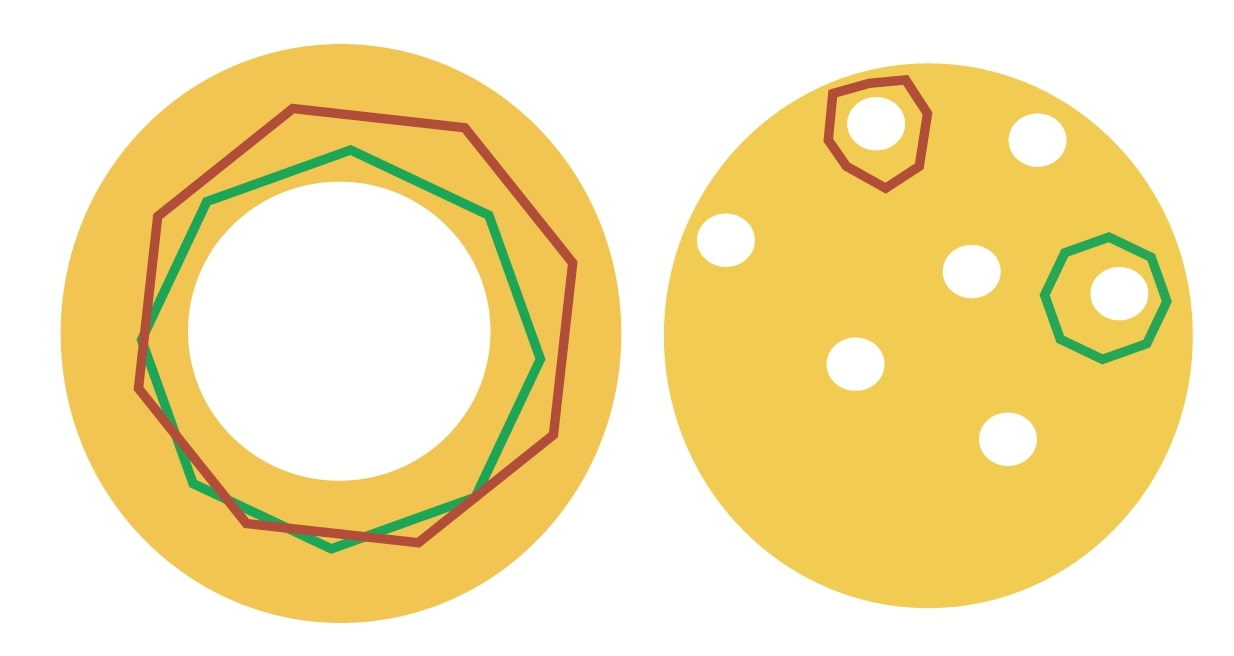
\includegraphics[width=0.8\textwidth]{figures/generatorExample.jpg}
%DIFDELCMD <     %%%
\DIFdelendFL \DIFaddbeginFL \includegraphics[width=0.8\textwidth]{figures/generatorExample (1).jpg}
    \DIFaddendFL \caption{Two disks (yellow) --- which we regard as 2-dimensional simplicial complexes, though the explicit decomposition into simplices is not shown --- with different numbers of holes (white) and cycle representatives (red or green) from \cite{Carlsson2009TopologyAD}. The disk on the left has a single 2-dimensional  ``hole'' ($\beta_1 = 1$), and the two loops around it are cycle representatives for the same homology class. Similarly, the disk on the right has seven ``holes'' ($\beta_1 = 7$) and the two loops shown are cycle representatives for different homology classes.
    }
    \label{fig:generatorExamples}
\end{figure}

 \begin{figure}[h!]
\begin{center}
\DIFdelbeginFL %DIFDELCMD < 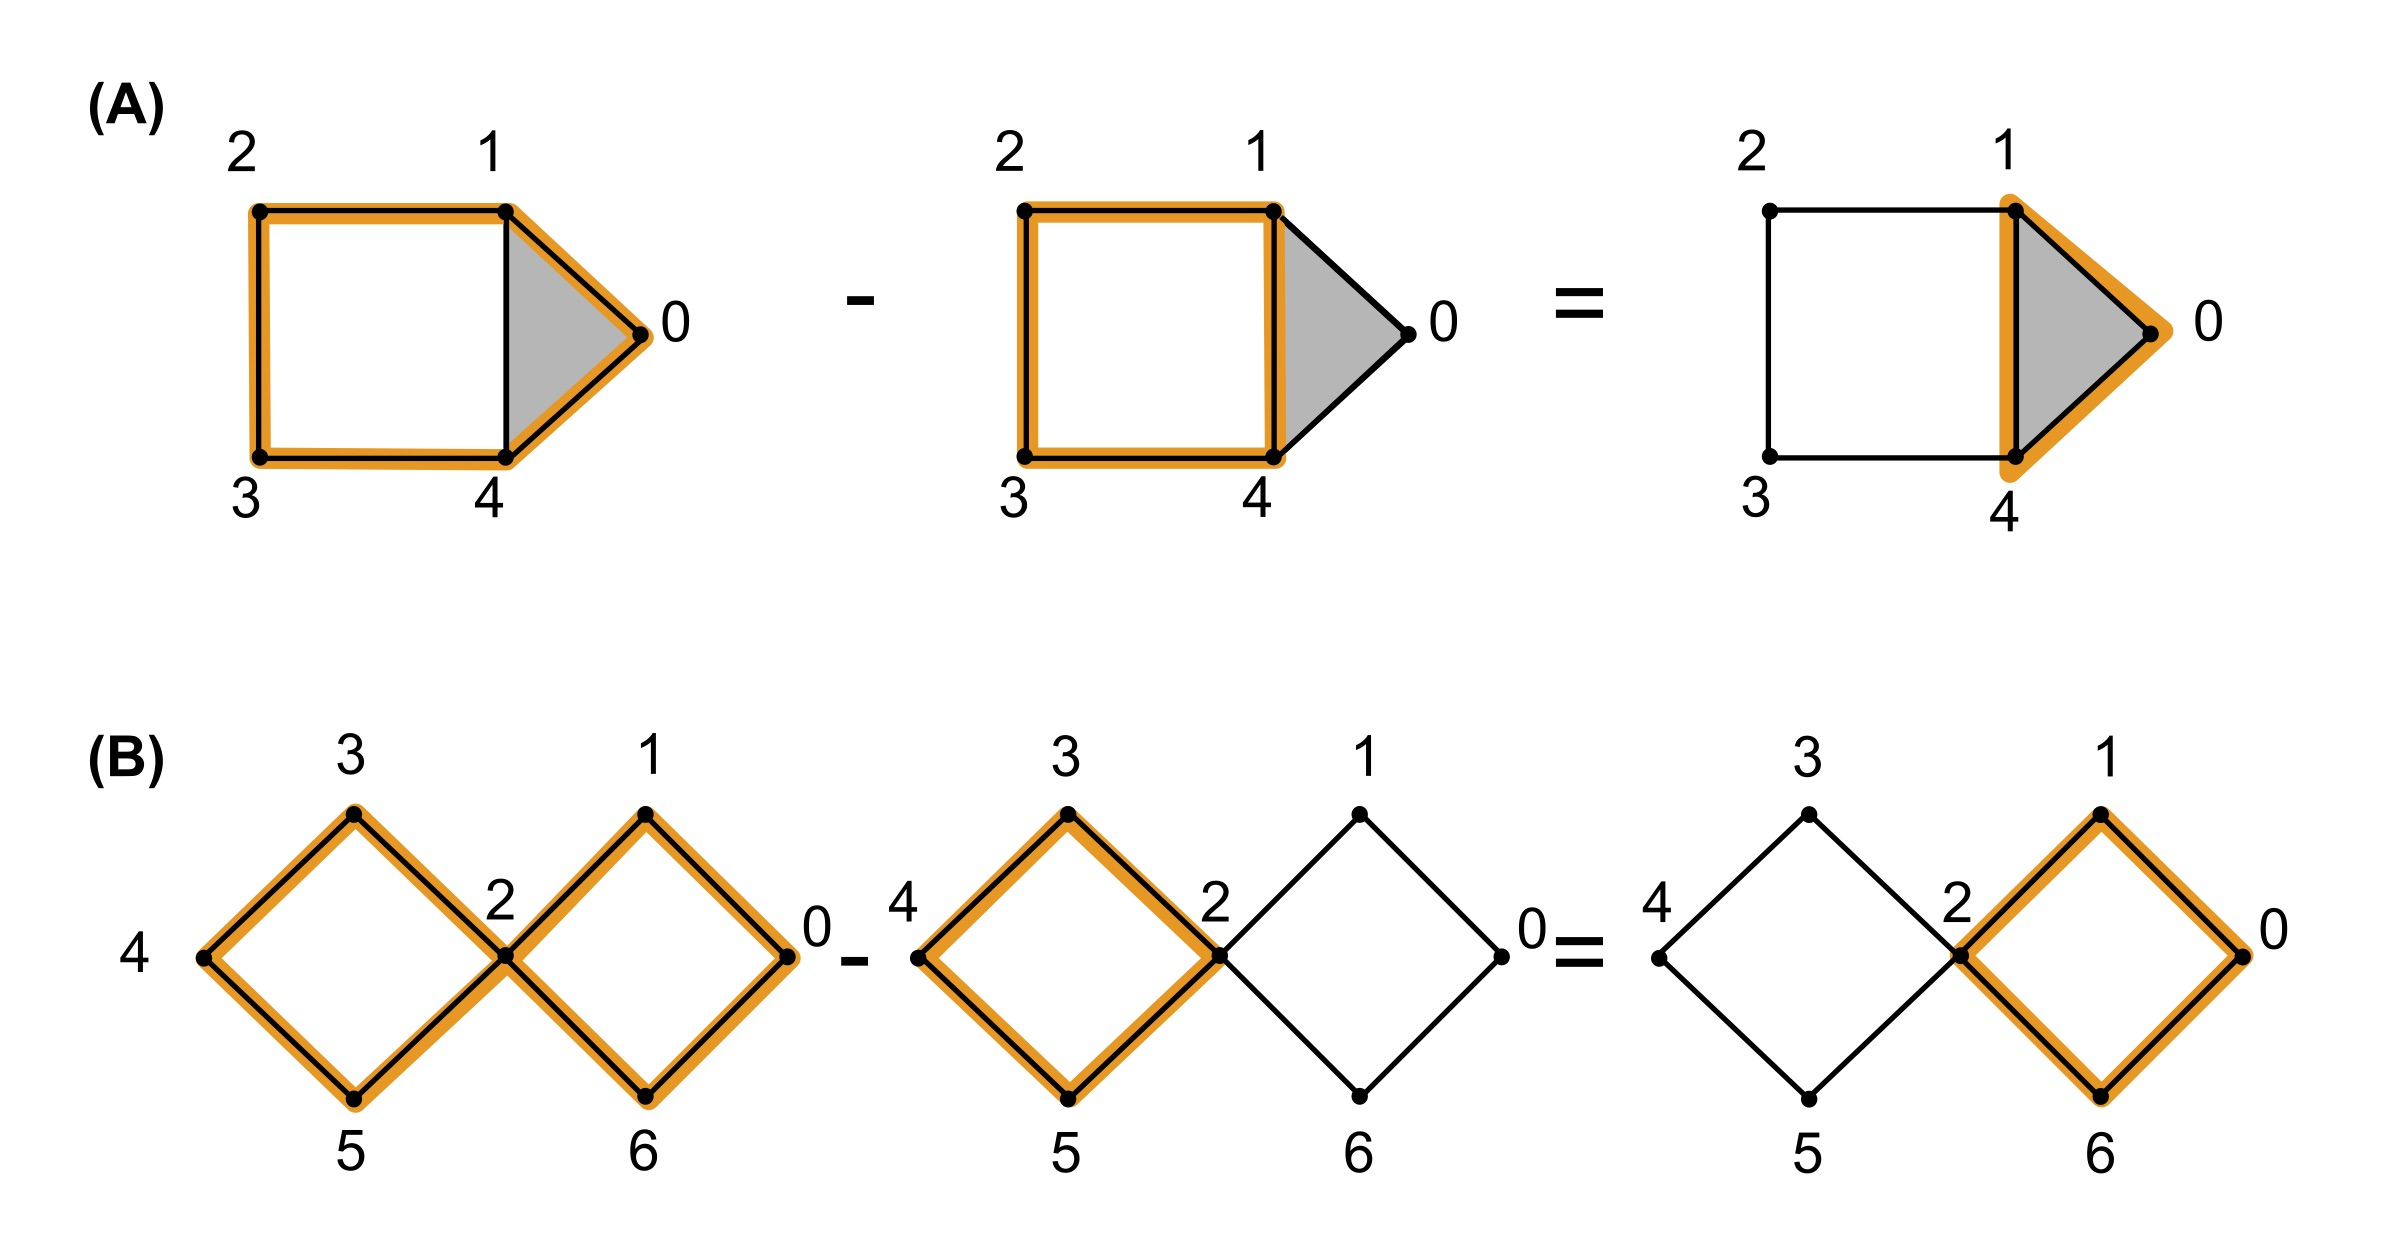
\includegraphics[width=1\textwidth]{figures/examplesorange.jpg} 
%DIFDELCMD < %%%
\DIFdelendFL \DIFaddbeginFL \includegraphics[width=1\textwidth]{figures/examplesorange (2).jpg} 
\DIFaddendFL \end{center}
\caption{We show an example of homologous cycles in \textbf{(A)}, taken from \cite{TZH15}. The 1-cycle $(0,1) + (1,2) + (2,3) + (3,4) - (0,4)$ and the 1-cycle $(1,2) + (2,3) + (3,4) - (4,1)$ are homologous because their difference is the boundary of $(0,1,4)$. Subfigure \textbf{(B)} shows an example of non-homologous cycles. The 1-cycle $(\sum_{i=0}^4 (i, i+1))-(5,2)+(2,6)-(0,6)$ and the 1-cycle $(2,3) + (3,4)+(4,5)-(2,5)$ are not homologous because their difference is a cycle $(0,1)+(1,2)+(2,6)-(0,6)$ which is not a linear combination of boundaries of 2-simplices. } \label{fig:boundaryexample}
\end{figure}

\begin{figure}[h!]
\begin{center}
\DIFdelbeginFL %DIFDELCMD < 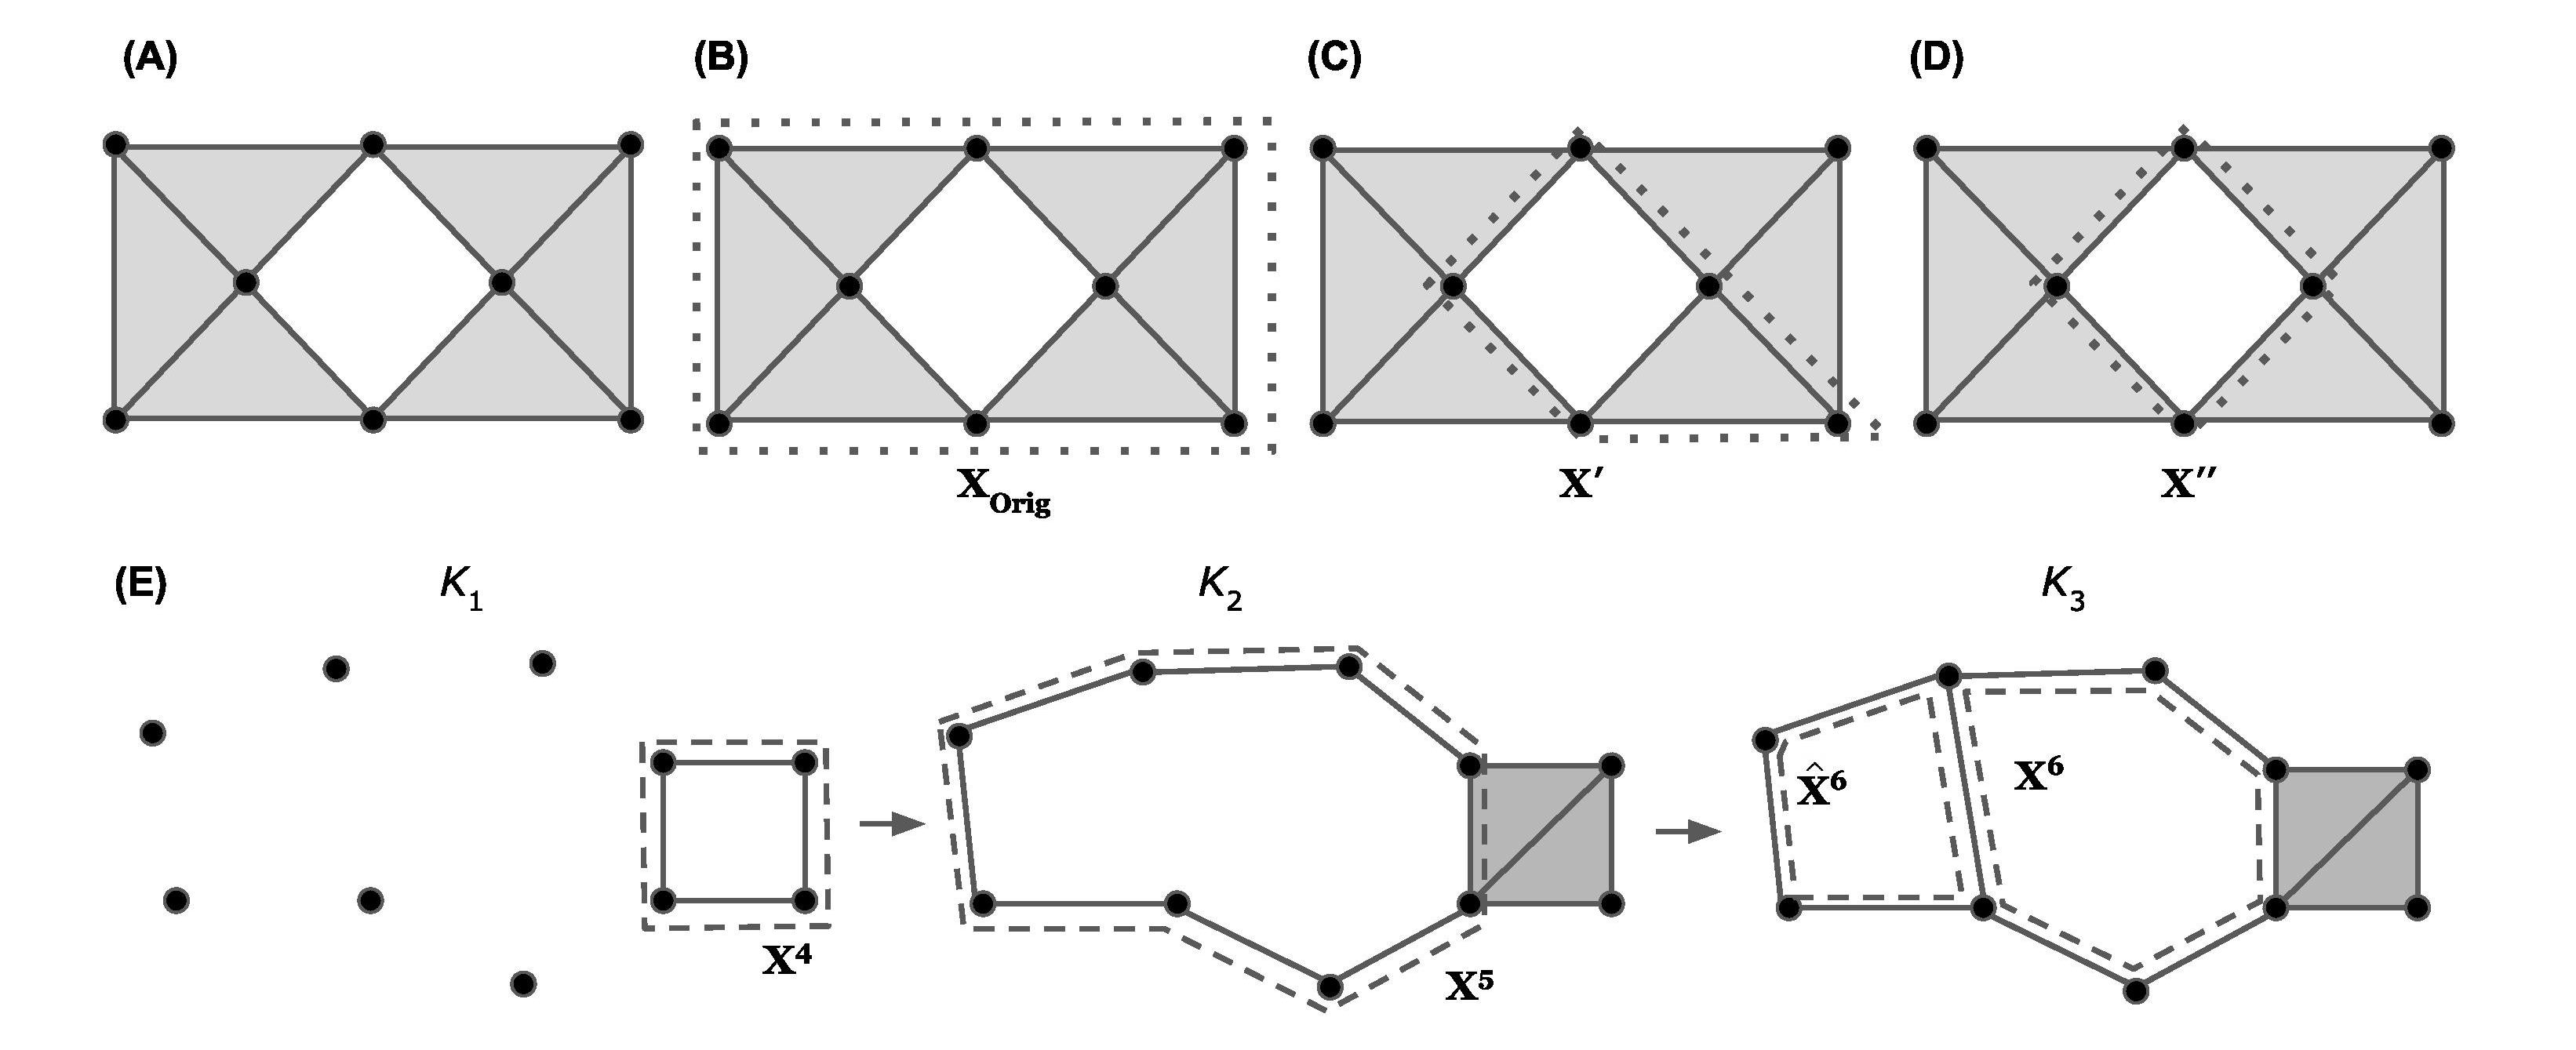
\includegraphics[width=1\textwidth]{figures/examples.jpg} 
%DIFDELCMD < %%%
\DIFdelendFL \DIFaddbeginFL \includegraphics[width=1\textwidth]{figures/examples (1).jpg} 
\DIFaddendFL \end{center}
\caption{Examples of optimizing a cycle representative (using the notion of minimizing edges) within the same homology class (\textbf{A-D}) and using a basis of cycle representatives (\textbf{E}), modified examples taken from \cite{Escolar2016} and \cite{Obayashi2018}. The dotted lines represent a cycle representative for the enclosed ``hole''. Intuitively, we consider $\optimalrep''$ in (\textbf{D}) as the optimal cycle representative since it consists of the smallest number of edges. Subfigure (\textbf{E}) shows a case where we optimize a cycle representative using a basis of cycle representatives. In (\textbf{E}), $\{\optimalrep^4, \optimalrep^5, \optimalrep^6\}$ is the original basis of cycle representatives. We can substitute $\optimalrep^6$ with $\hat{\optimalrep}^6$, which we can obtain by adding $\optimalrep^5$ to $\optimalrep^6$, and thus obtain $\{\optimalrep^4, \optimalrep^5, \hat{\optimalrep}^6\}$ as the new basis of cycle representatives.}\label{fig:example-optimal}
\end{figure}


\begin{figure}[h!]
\begin{center}
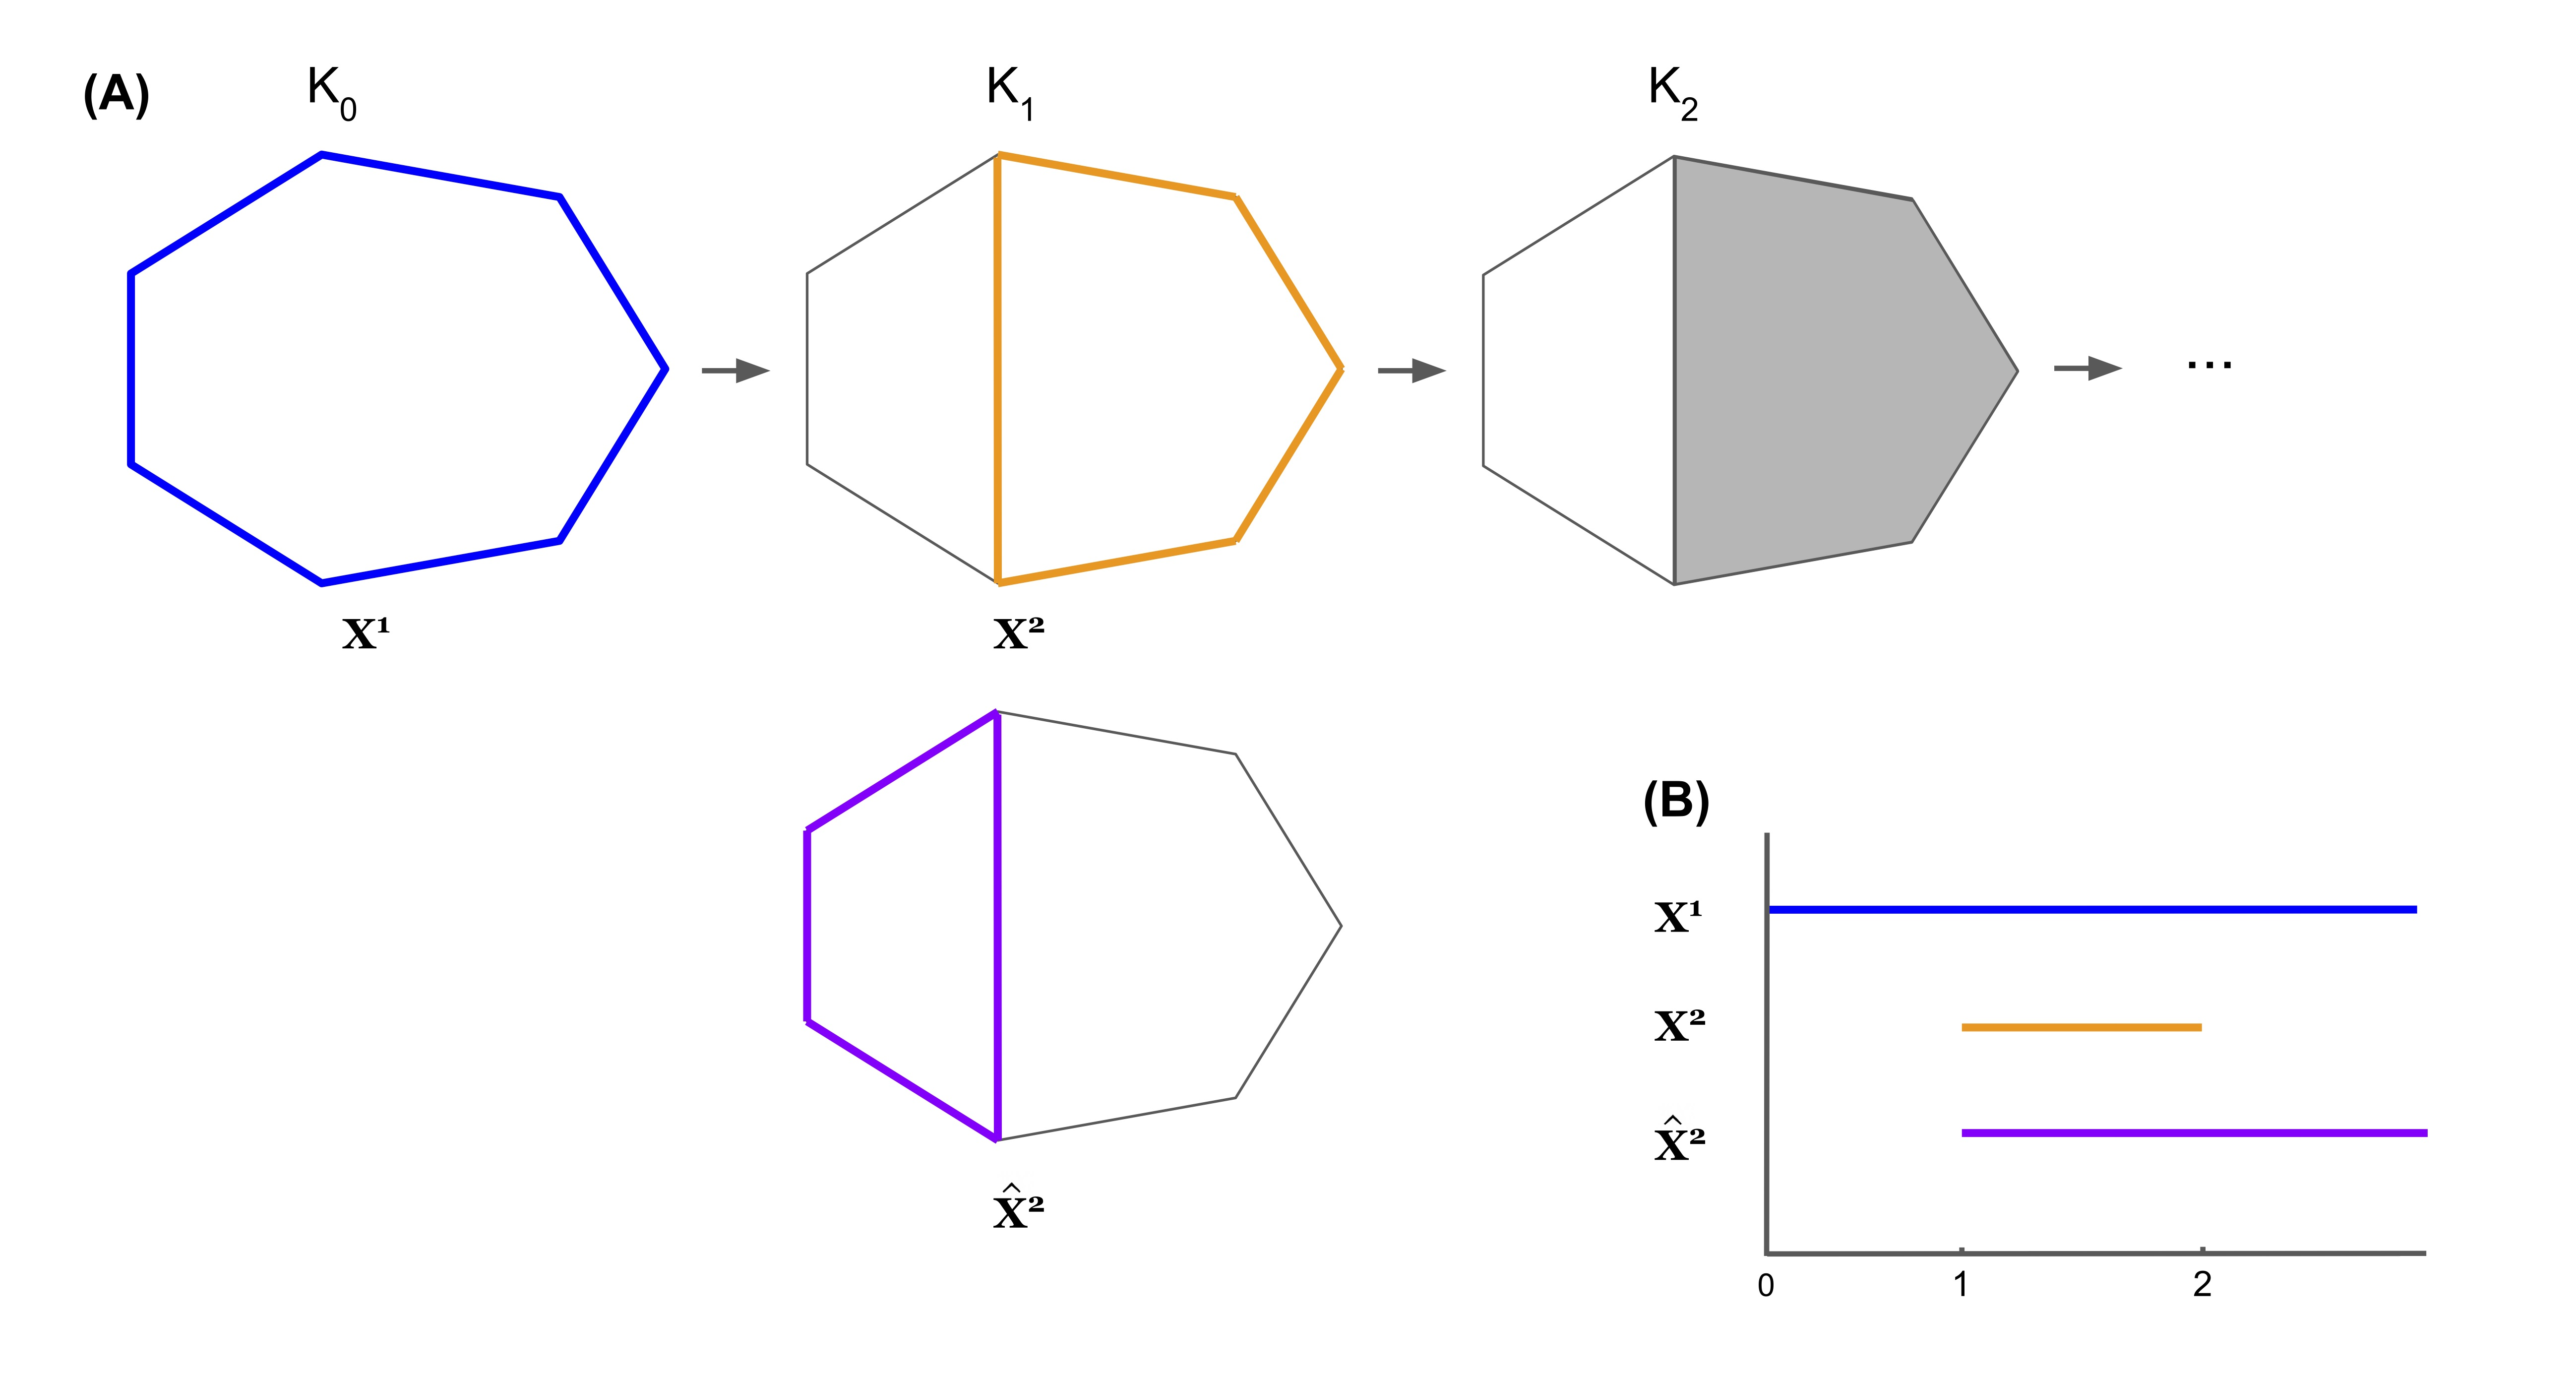
\includegraphics[width=1\textwidth]{figures/gregExample.jpg}
\end{center}
\caption{An example where the optimal cycles obtained from \pr \eqref{eq:escolarargmin} do not form a persistent homological cycle basis. The thickened colored cycles in Subfigure (\textbf{A}) represent a cycle representative for the hole it encloses, and the bar with the corresponding color in Subfigure (\textbf{B}) records the lifespan of the cycle. In Subfigure (\textbf{A}), we see $\persinterval(\optimalrep^1) = [0,\infty), \persinterval(\optimalrep^2) = [1,2).$ Then, $\{\optimalrep^1, \optimalrep^2\}$ forms a basis for the persistent homological cycles. The cycle representative $\hat \optimalrep^2$ is an optimal cycle representative obtained by solving \pr (\ref{eq:filteredminimalbasis}) for the filtered simplicial complex $K_2$. However, $\persinterval(\hat \optimalrep_2) = [1, \infty)$, and thus  $\{\optimalrep^1, \hat \optimalrep^2\}$ is no longer a persistent homological cycle basis.} \label{fig:example-persBasis}
\end{figure}


 \begin{figure}[h!]
\begin{center}
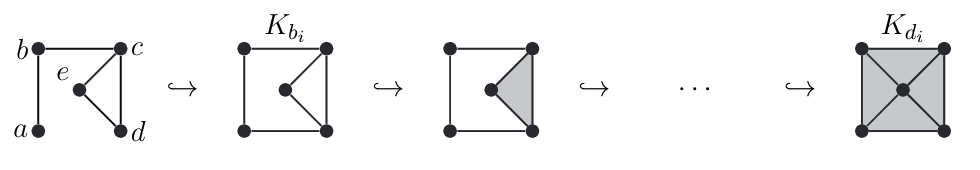
\includegraphics[width=1\textwidth]{figures/volumeexample.jpg}
\end{center}
\caption{A situation in which a volume-optimal cycle is different from the uniform minimal cycle. Consider the filtered simplicial complex pictured. For the persistence interval $[b_i,d_i)$, the cycle with minimal $0$-norm (fewest number of edges) is $(a,b) + (b,c) + (c,d)  + (d,a)$.
However, the volume-optimal cycle would be found as follows: considering $K_{d_i}$, we must find the fewest $2$-simplices whose boundary captures the persistence interval. In this case, we would have an optimal volume $(a,b,e) + (b,c,e) + (a,d,e)$ and volume-optimal cycle $(a,b) + (b,c) + (c,e) + (e,d) + (d,a)$. 
}\label{fig:volumeoptimal}
\end{figure} 

\begin{figure}[h!]
\begin{center}
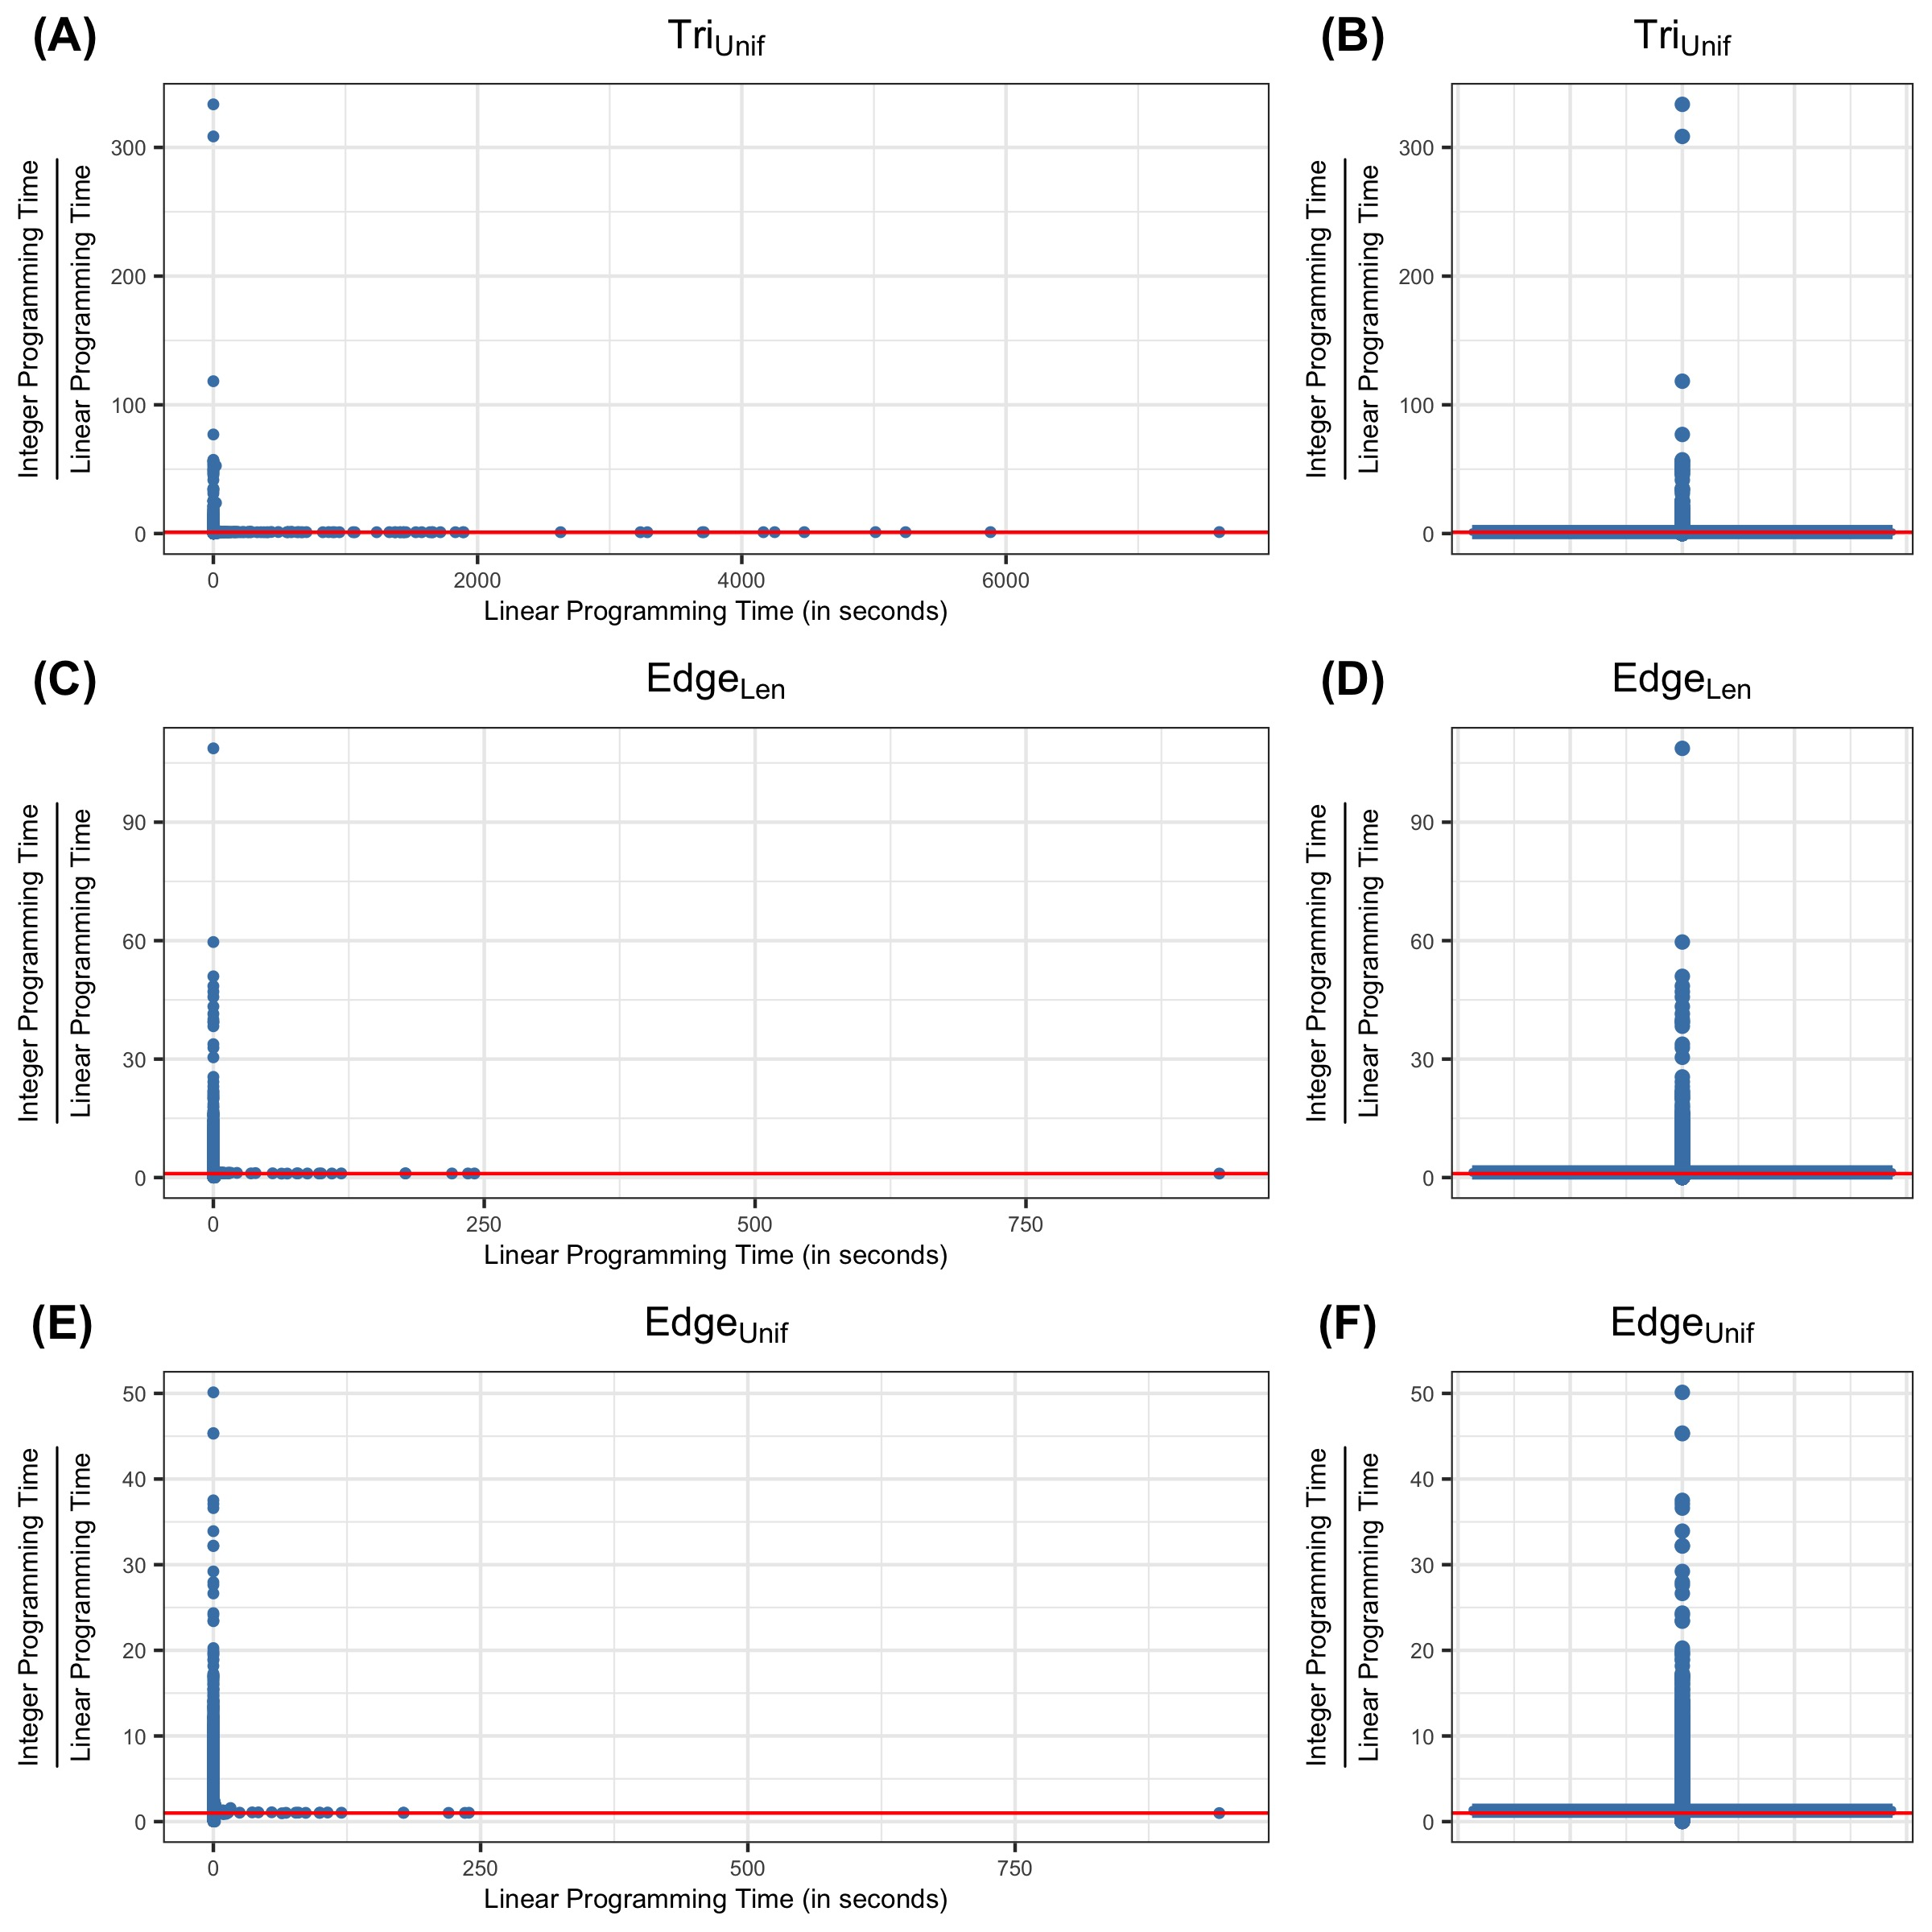
\includegraphics[width=\textwidth]{figures/IPvsLP.jpg} 
\end{center}
 \caption{ 
 Ratio between the computation time of solving an integer programming problem \DIFaddbeginFL \DIFaddFL{(}\DIFaddendFL Programs \ref{itm:tri_IU}, \ref{itm:edge_IL}, \ref{itm:edge_IU}\DIFaddbeginFL \DIFaddFL{) }\DIFaddendFL and the computation time of solving a linear programming problem \DIFaddbeginFL \DIFaddFL{(}\DIFaddendFL Programs \ref{itm:tri_NIU}, \ref{itm:edge_NIL}, \ref{itm:edge_NIU}\DIFaddbeginFL \DIFaddFL{) }\DIFaddendFL for all the cycle representatives from data sets described in \DIFdelbeginFL \DIFdelFL{\se \ref{tab:realworldata} }\DIFdelendFL \DIFaddbeginFL \DIFaddFL{Sections \ref{sec: realworlddata}, \ref{sec: randompointclouds}, }\DIFaddendFL and \DIFdelbeginFL \DIFdelFL{\se \ref{tab:distributiondata}}\DIFdelendFL \DIFaddbeginFL \DIFaddFL{\ref{sec:erdos}}\DIFaddendFL . Subfigures  \textbf{(A), (C), (E)} plot the data using scatter plots and subfigures  \textbf{(B), (D), (F)} show the same data using box plots. The vertical axis represents the ratio between the integer programming time and linear programming time of optimizing a cycle representative and the horizontal axis represents the computation time to solve the linear program. The red line in each subfigure represents the horizontal line $y=1$, where the time for each optimization is equivalent. As we can see from the box plots, the ratio between the computation time of integer programming and linear programming for most of the cycle representatives ($>50\%$) center around $1$.}\label{fig:lp_mip_ratio_df}
\end{figure}

%DIF >   \begin{landscape}
%DIF >  \begin{figure}[hbt!]
%DIF >  \begin{center}
%DIF >  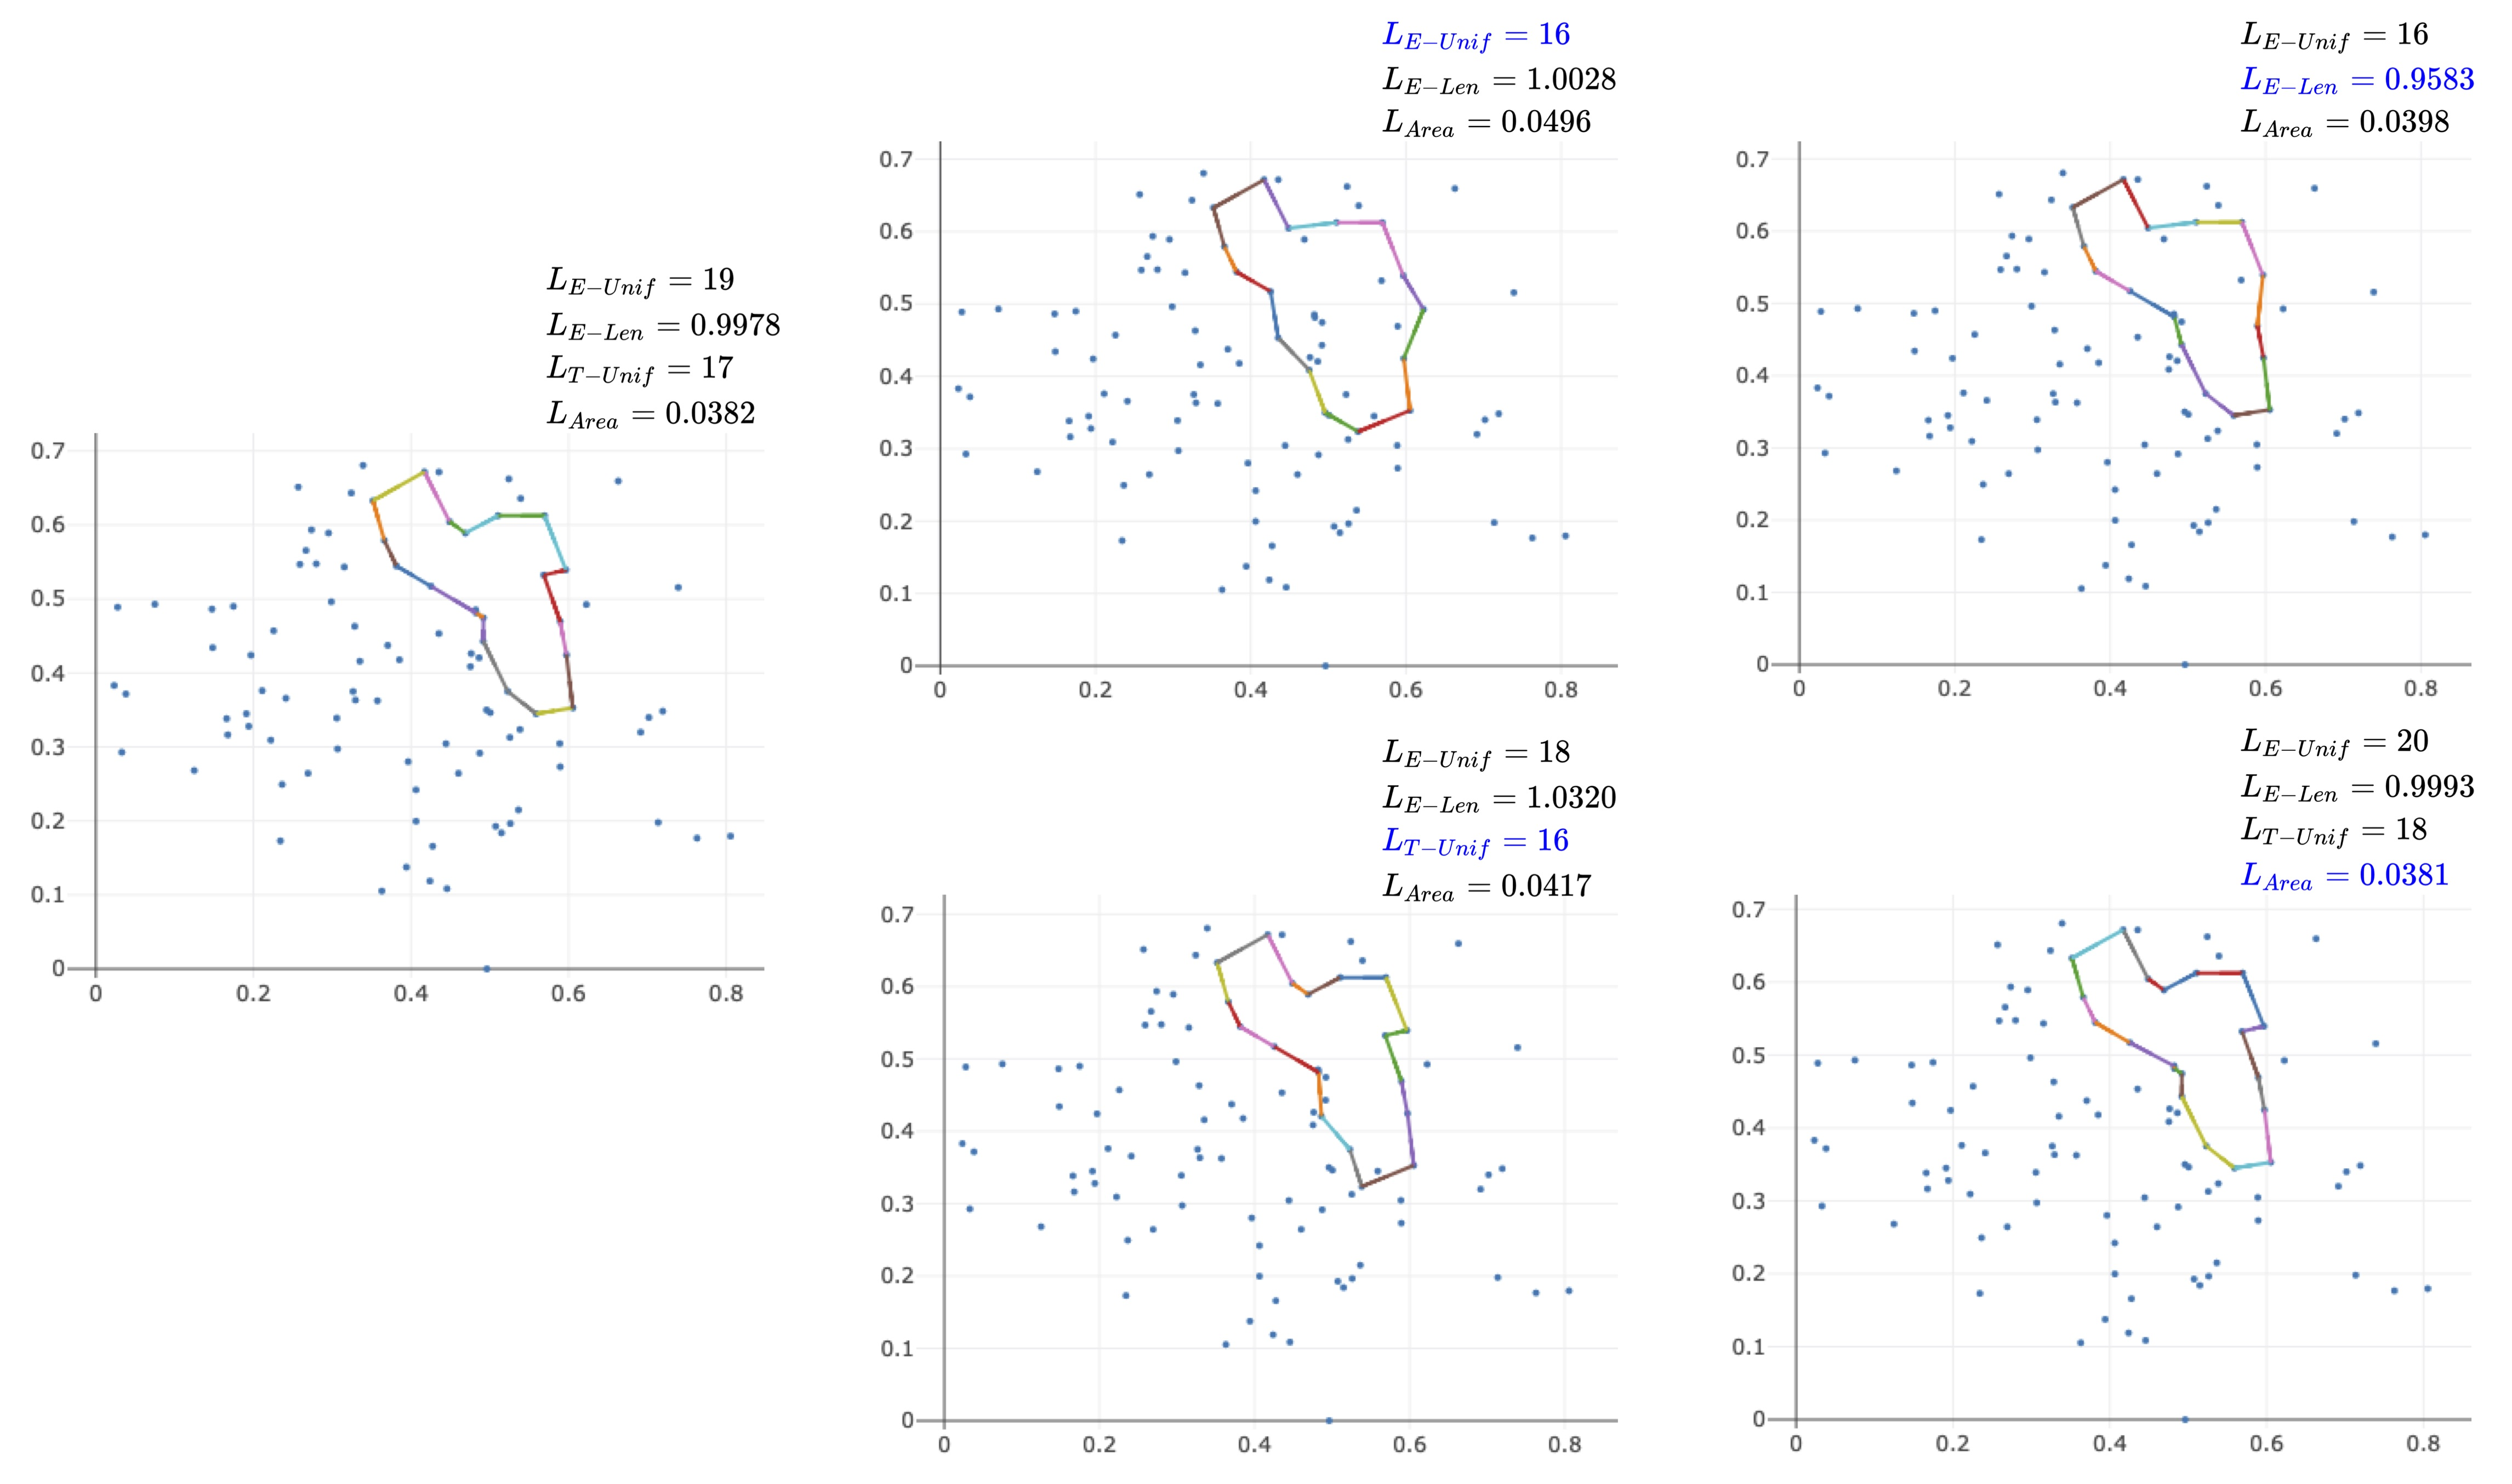
\includegraphics[width=\textwidth]{figures/examples_new.jpg}
%DIF >  \end{center}
%DIF >  \caption{Examples of different optimal cycles and cost against different loss functions using a point cloud of $100$ points with ambient dimension $2$ randomly drawn from a normal distribution. The upper left corner of each subfigure labels the optimization algorithm used to optimize the original cycle representative. The upper right corner of each subfigure records the different measures of the size of the optimal representative. Blue text represents the measure an algorithm sets out to optimize. \LL{Updated. Found a maybe better example, see the next figure} 
%DIF >  }\label{fig:Examplesofeachoptimalcycles} 
%DIF >  \end{figure}
%DIF >  \end{landscape}
\DIFaddbegin 

\DIFaddend \begin{landscape}
\begin{figure}[hbt!]
\begin{center}
\DIFdelbeginFL %DIFDELCMD < \includegraphics[width=\textwidth]{figures/examples (1).jpg}
%DIFDELCMD < %%%
\DIFdelendFL \DIFaddbeginFL 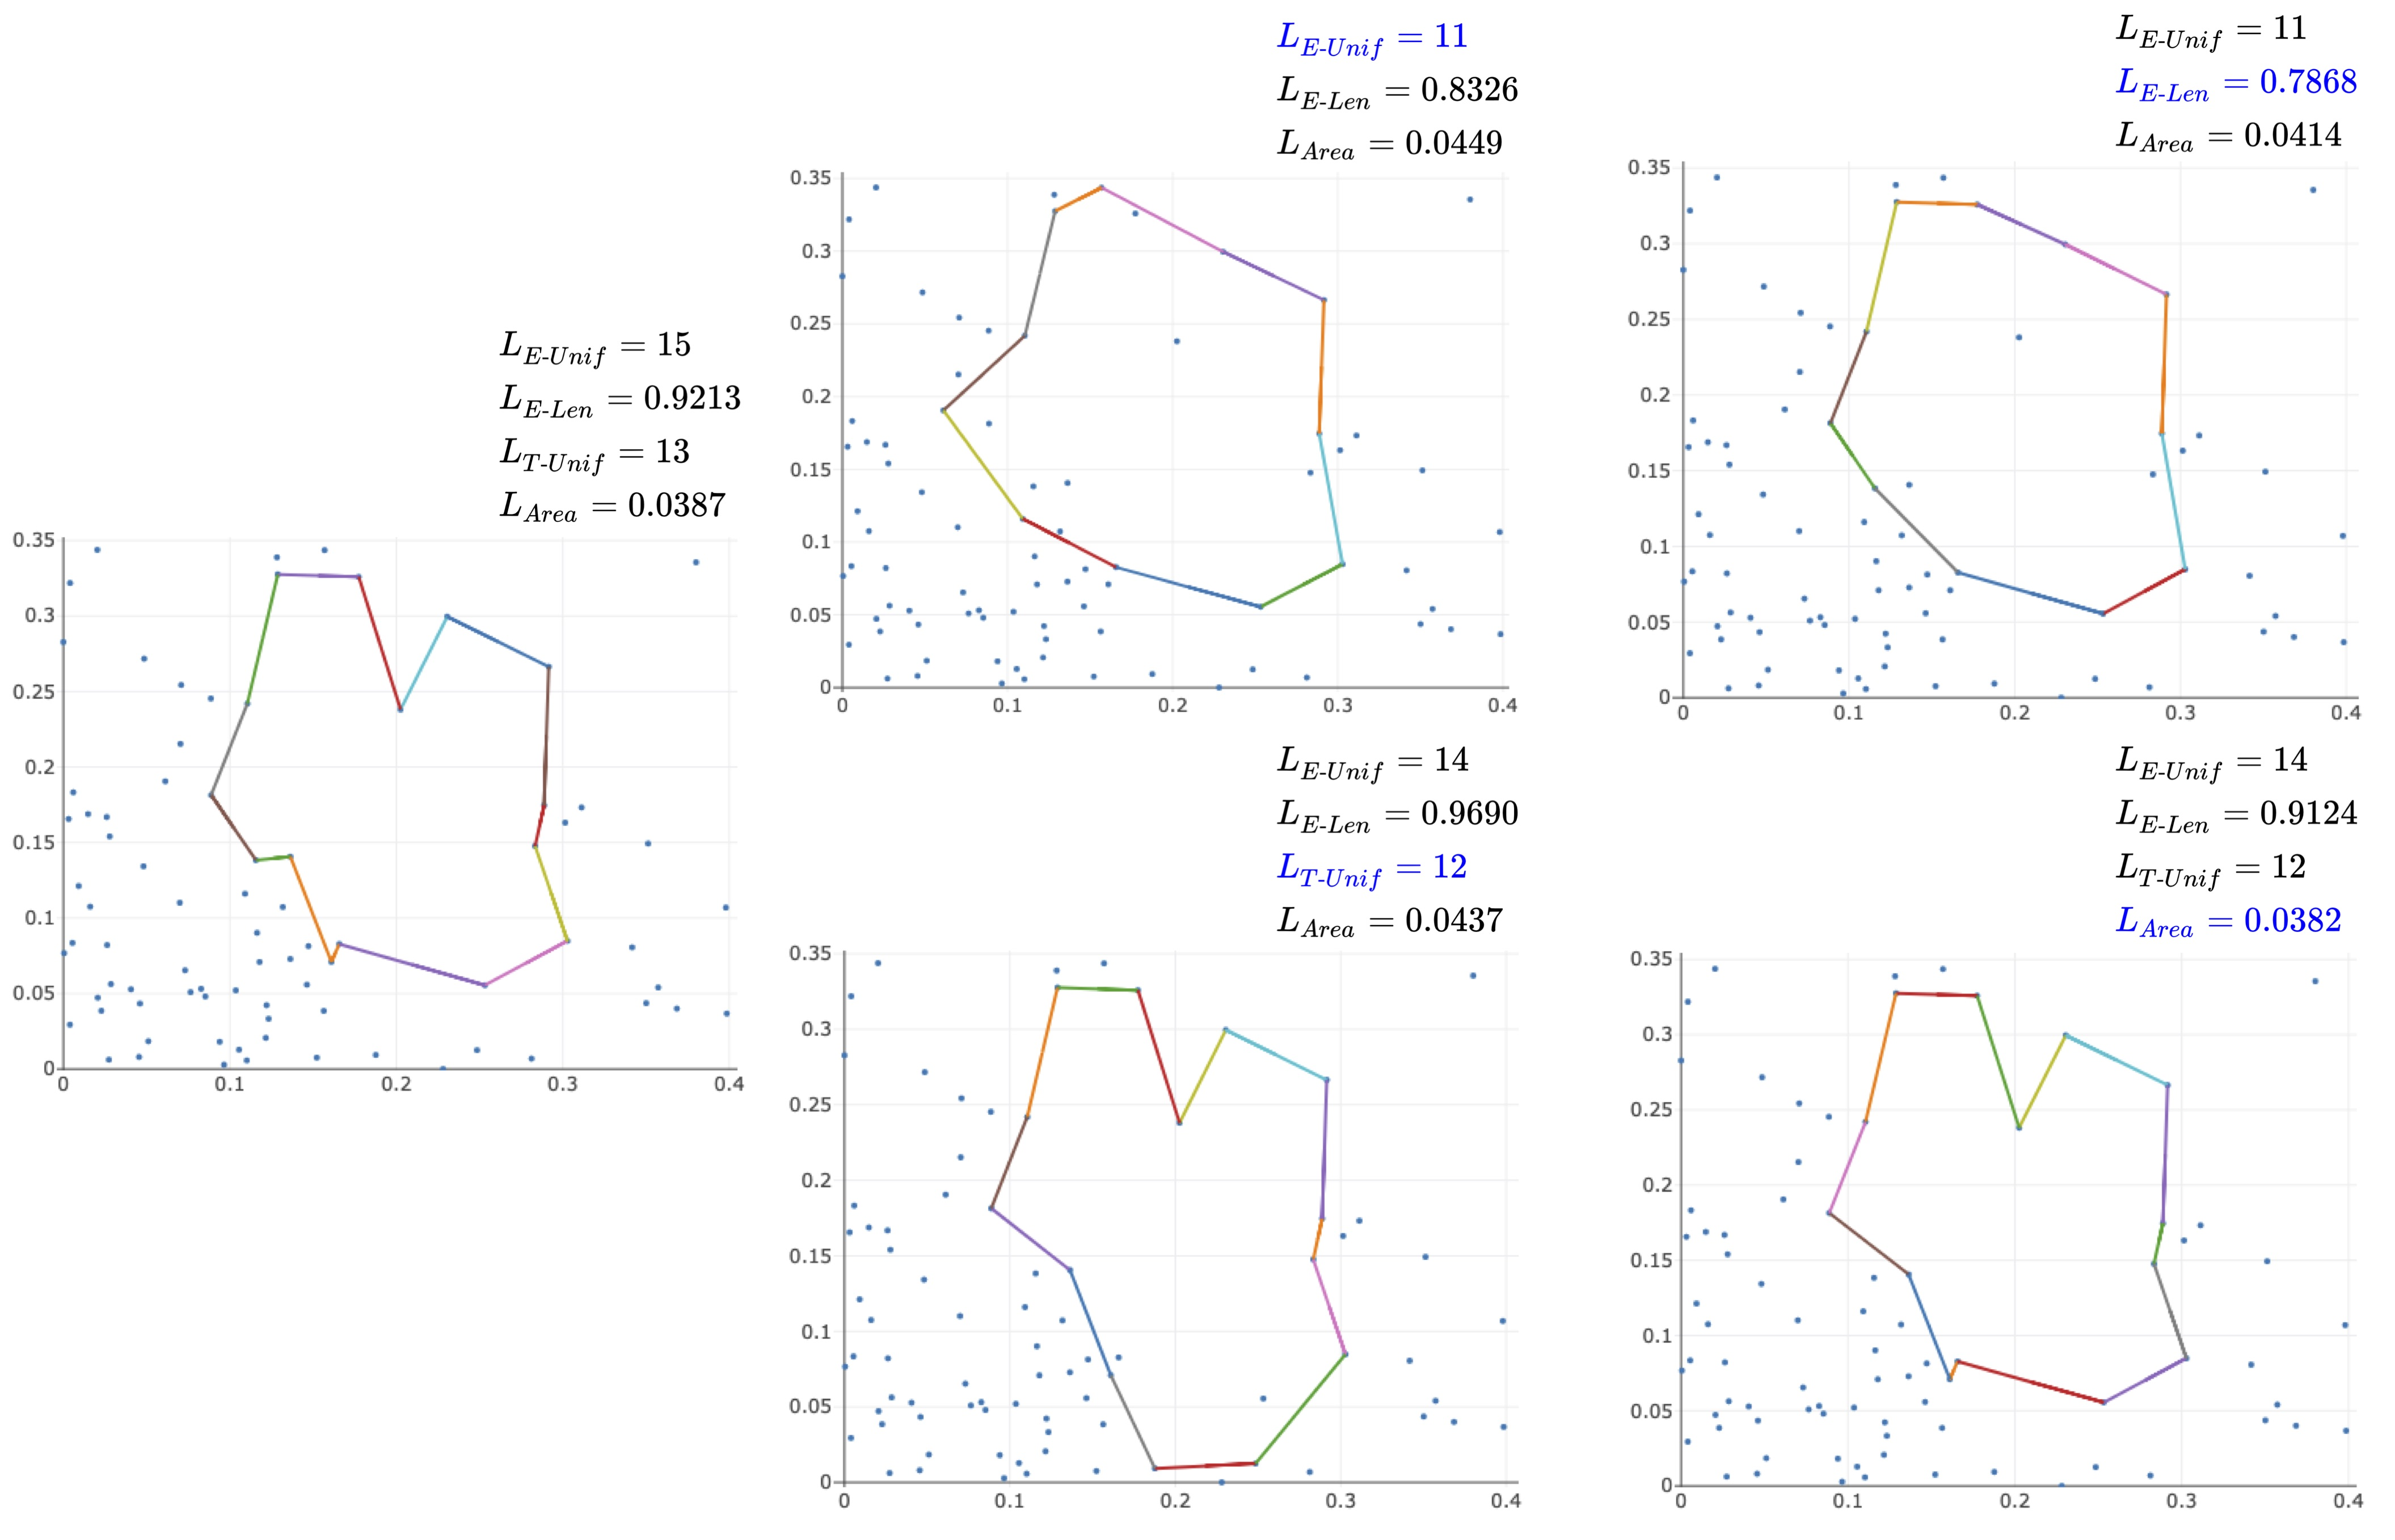
\includegraphics[width=\textwidth]{figures/examples_gamma.jpg}
\DIFaddendFL \end{center}
\caption{Examples of different optimal cycles and cost against different loss functions using a point cloud of $100$ points with ambient dimension $2$ randomly drawn from a normal distribution. The upper left corner of each subfigure labels the optimization algorithm used to optimize the original cycle representative. The upper right corner of each subfigure records the different measures of the size of the optimal representative. Blue text represents the measure an algorithm sets out to optimize. 
}\label{fig:Examplesofeachoptimalcycles} 
\end{figure}
\end{landscape}

\begin{figure}[h!]
\begin{center}
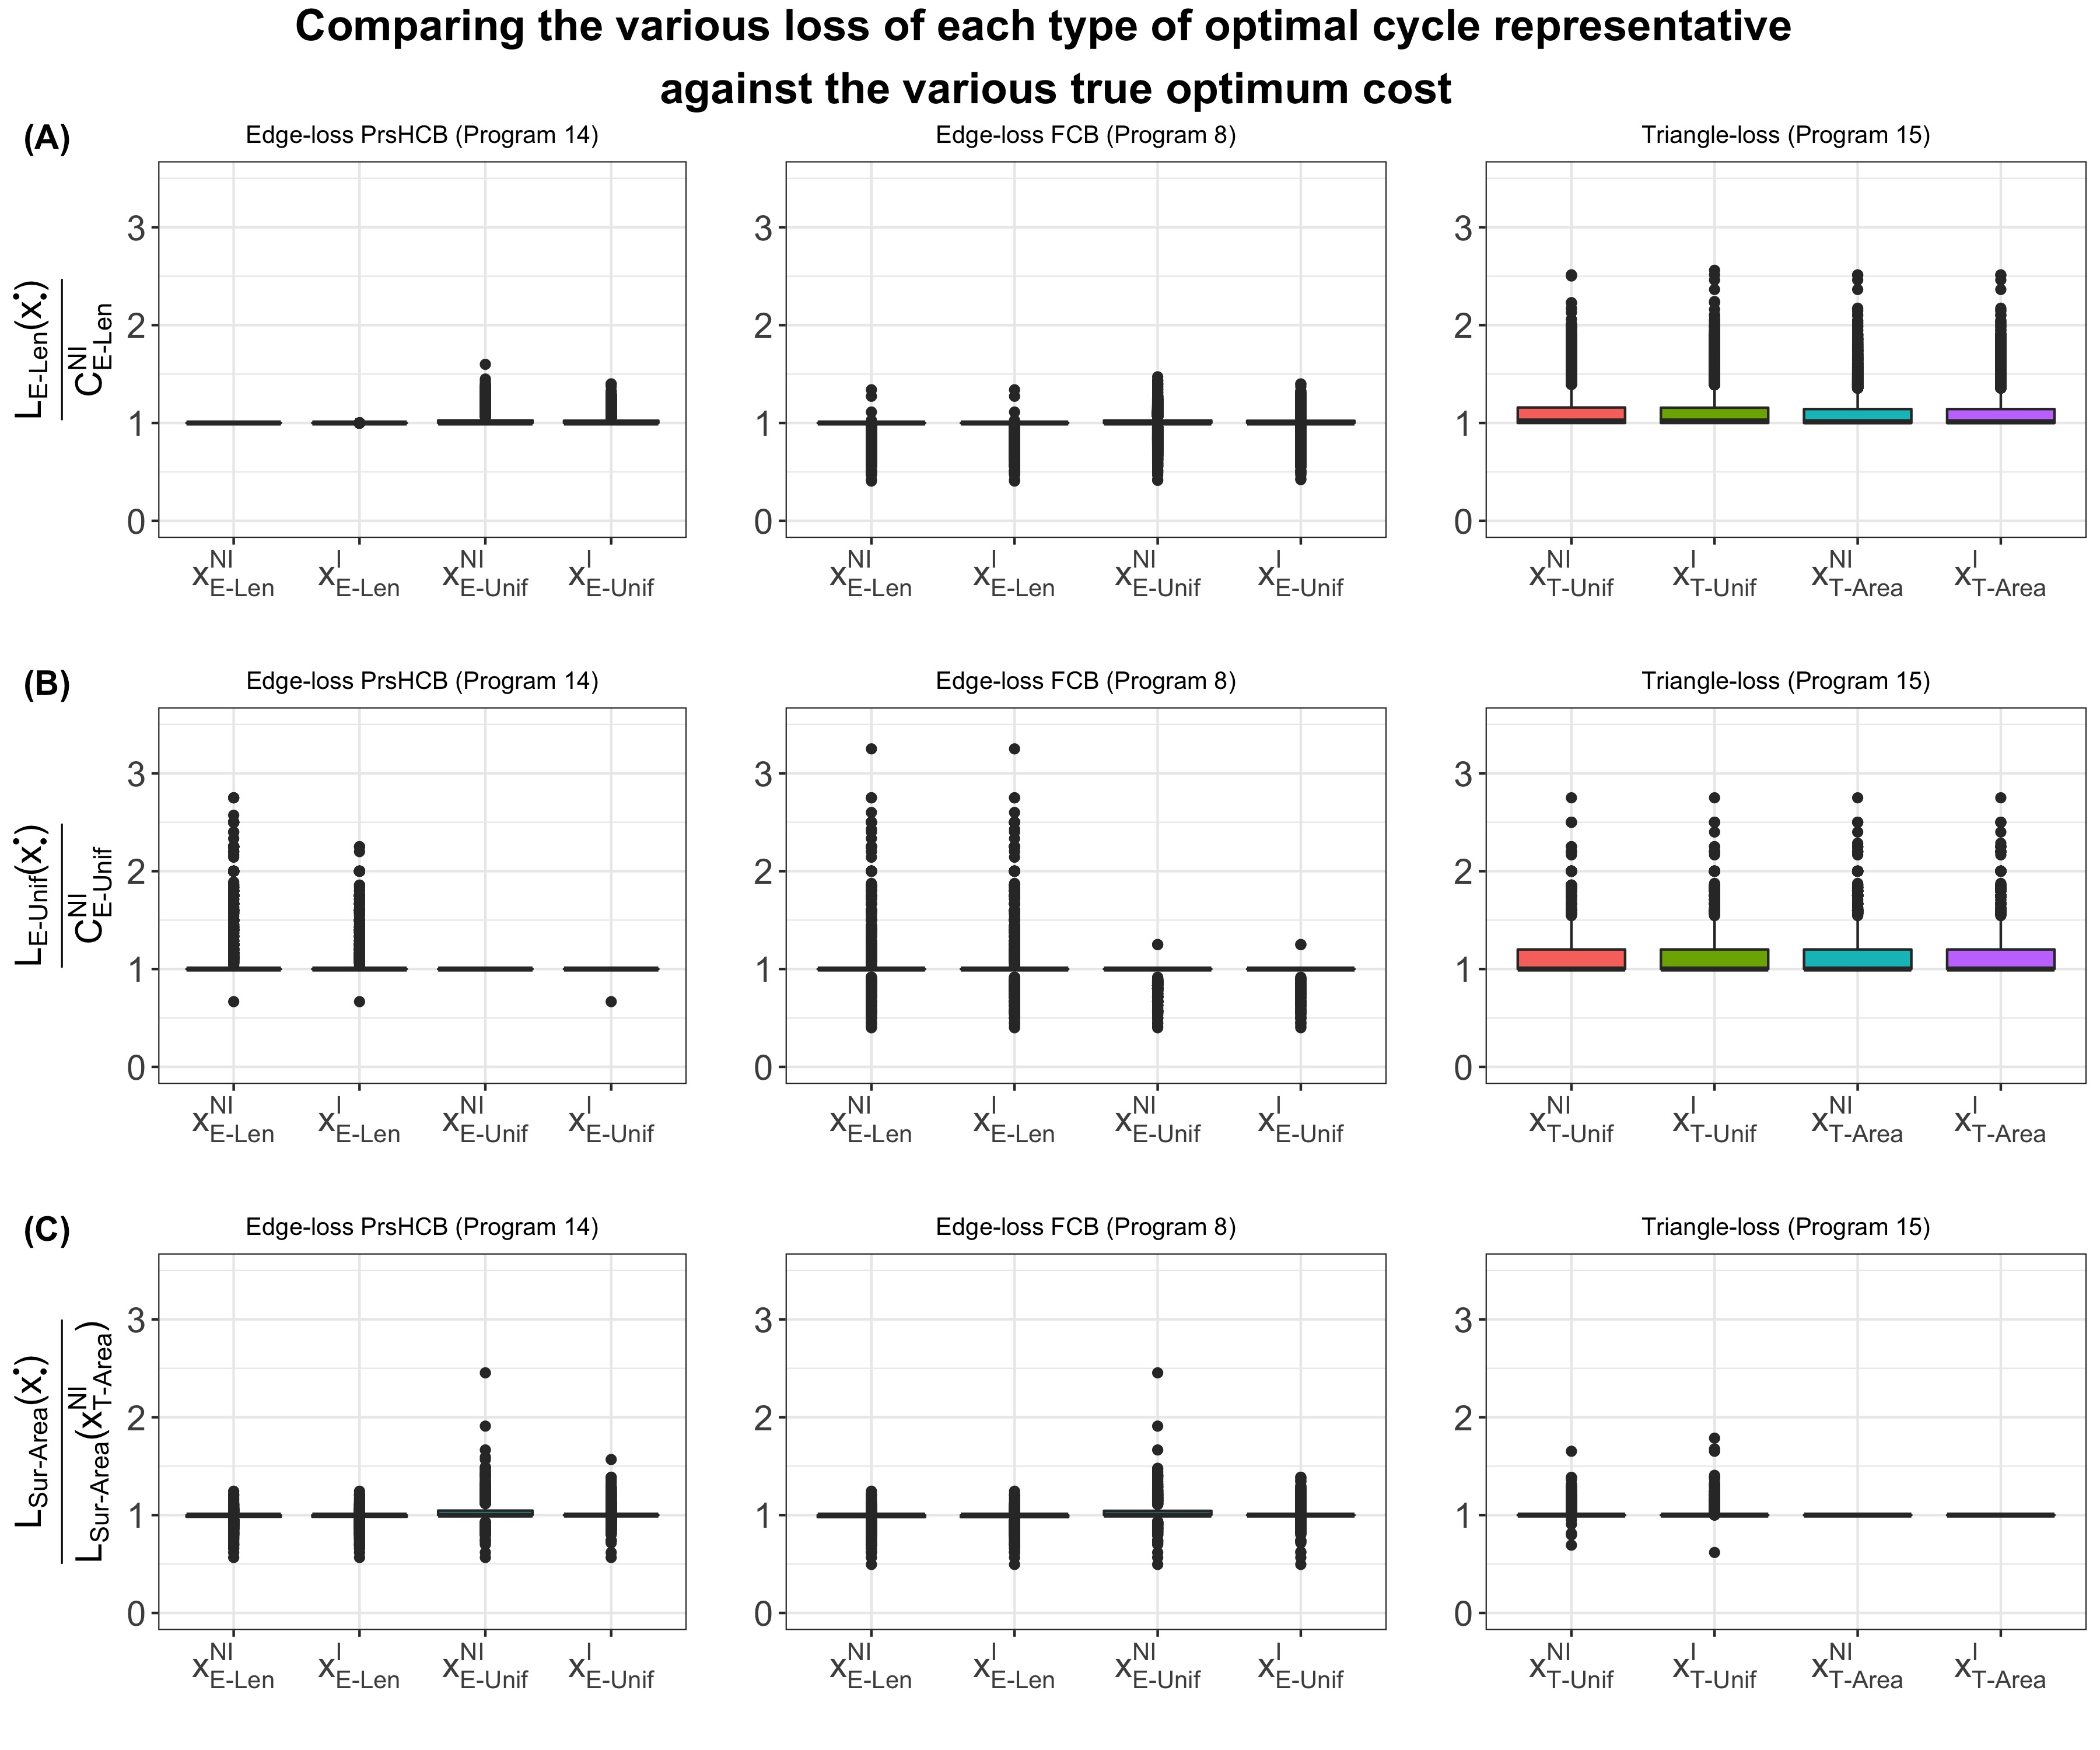
\includegraphics[width=\textwidth]{figures/length_area_edge.jpg}
\end{center}
\caption{Box plots of the ratios between (\textbf{A}) $L_{E\text{-}Len}(\optimalrep_\bullet^\bullet)$ and $C_{E\text{-}Len}$,  \textbf{(B)} $L_{E\text{-}Unif}(\optimalrep_\bullet^\bullet)$ and $C_{E\text{-}Unif}$, and  \textbf{(C)} $L_{T\text{-}Area}(\optimalrep_\bullet^\bullet)$ and $C_{T\text{-}Area}$. 
The horizontal axis is the type of optimal representative, $\optimalrep_\bullet^\bullet$, and the vertical axis is the ratio between the loss of each type of optimal representative over the actual cost of the optimal representative of the same loss function, i.e. the $\setofpersistenthcyclebases$ cycles which are solutions to Programs \ref{itm:edge_NIU}, \ref{itm:edge_NIL}, \ref{itm:tri_NIA}.
In \se \ref{coefficient}, we discussed that the optimum cost is the same whether we require an integer solution or not for essentially all solutions for \pr \eqref{eq:edgelossgeneral}, \pr \DIFdelbeginFL \DIFdelFL{\ref{eq:escolarargmin}}\DIFdelendFL \DIFaddbeginFL \eqref{eq:escolarargmin}\DIFaddendFL , and the uniform-weighted triangle-loss method, resulting in two columns in the first two rows having ratio 1. The data used in \textbf{(A)} and \textbf{(B)} aggregate over all data described in \ref{sec: realworlddata} and \ref{sec: randompointclouds}. The data used in \textbf{(C)} aggregate the $190$ cycle representatives from $10$ point clouds from a normal distribution with ambient dimension of $2$. True area represents the total area enclosed by the representative, while $C_{Area}\NI$ represents the area of the area-weighted triangle-loss optimal cycle minimizing \ref{itm:tri_NIA}. We observe that some edge-loss optimal cycles and triangle-loss optimal cycles requiring integral solutions have an area smaller than that of the area-weighted triangle-loss optimal cycle. Refer to Figure \ref{fig:areaExample} and \se  \ref{sec:comparing optimal generators against different loss functions} to see why this may happen. \DIFaddbeginFL \LL{In the first plot on the second row, the original cycle representative where $\optimalrep_{E\text{-}Unif}^{NI}$ does not attain the optimum uniform-weighted edge-loss is a generator for the \textbf{C.elegans} data set, where there are duplicate intervals and $\optimalrep_{E\text{-}Unif}^{NI}$ has entries in $\{-0.5, 0, 0.5\}$ while $\optimalrep_{E\text{-}Len}^{NI}$, $\optimalrep_{E\text{-}Len}^{I}$, and $\optimalrep_{E\text{-}Unif}^{I}$ all have entries in $\{-1, 0,1\}$. See a more detailed discussion in \se \ref{duplicate intervals}}\DIFaddFL{. 
}\DIFaddendFL }
 \label{fig:lengthcocmpare}
\end{figure}
 \newpage 
 \DIFaddbegin 

\DIFaddend \begin{figure}[h!]
\begin{center}
\DIFdelbeginFL %DIFDELCMD < \includegraphics[width=\textwidth]{figures/loopsBreakdown (1).jpg}
%DIFDELCMD < %%%
\DIFdelendFL \DIFaddbeginFL 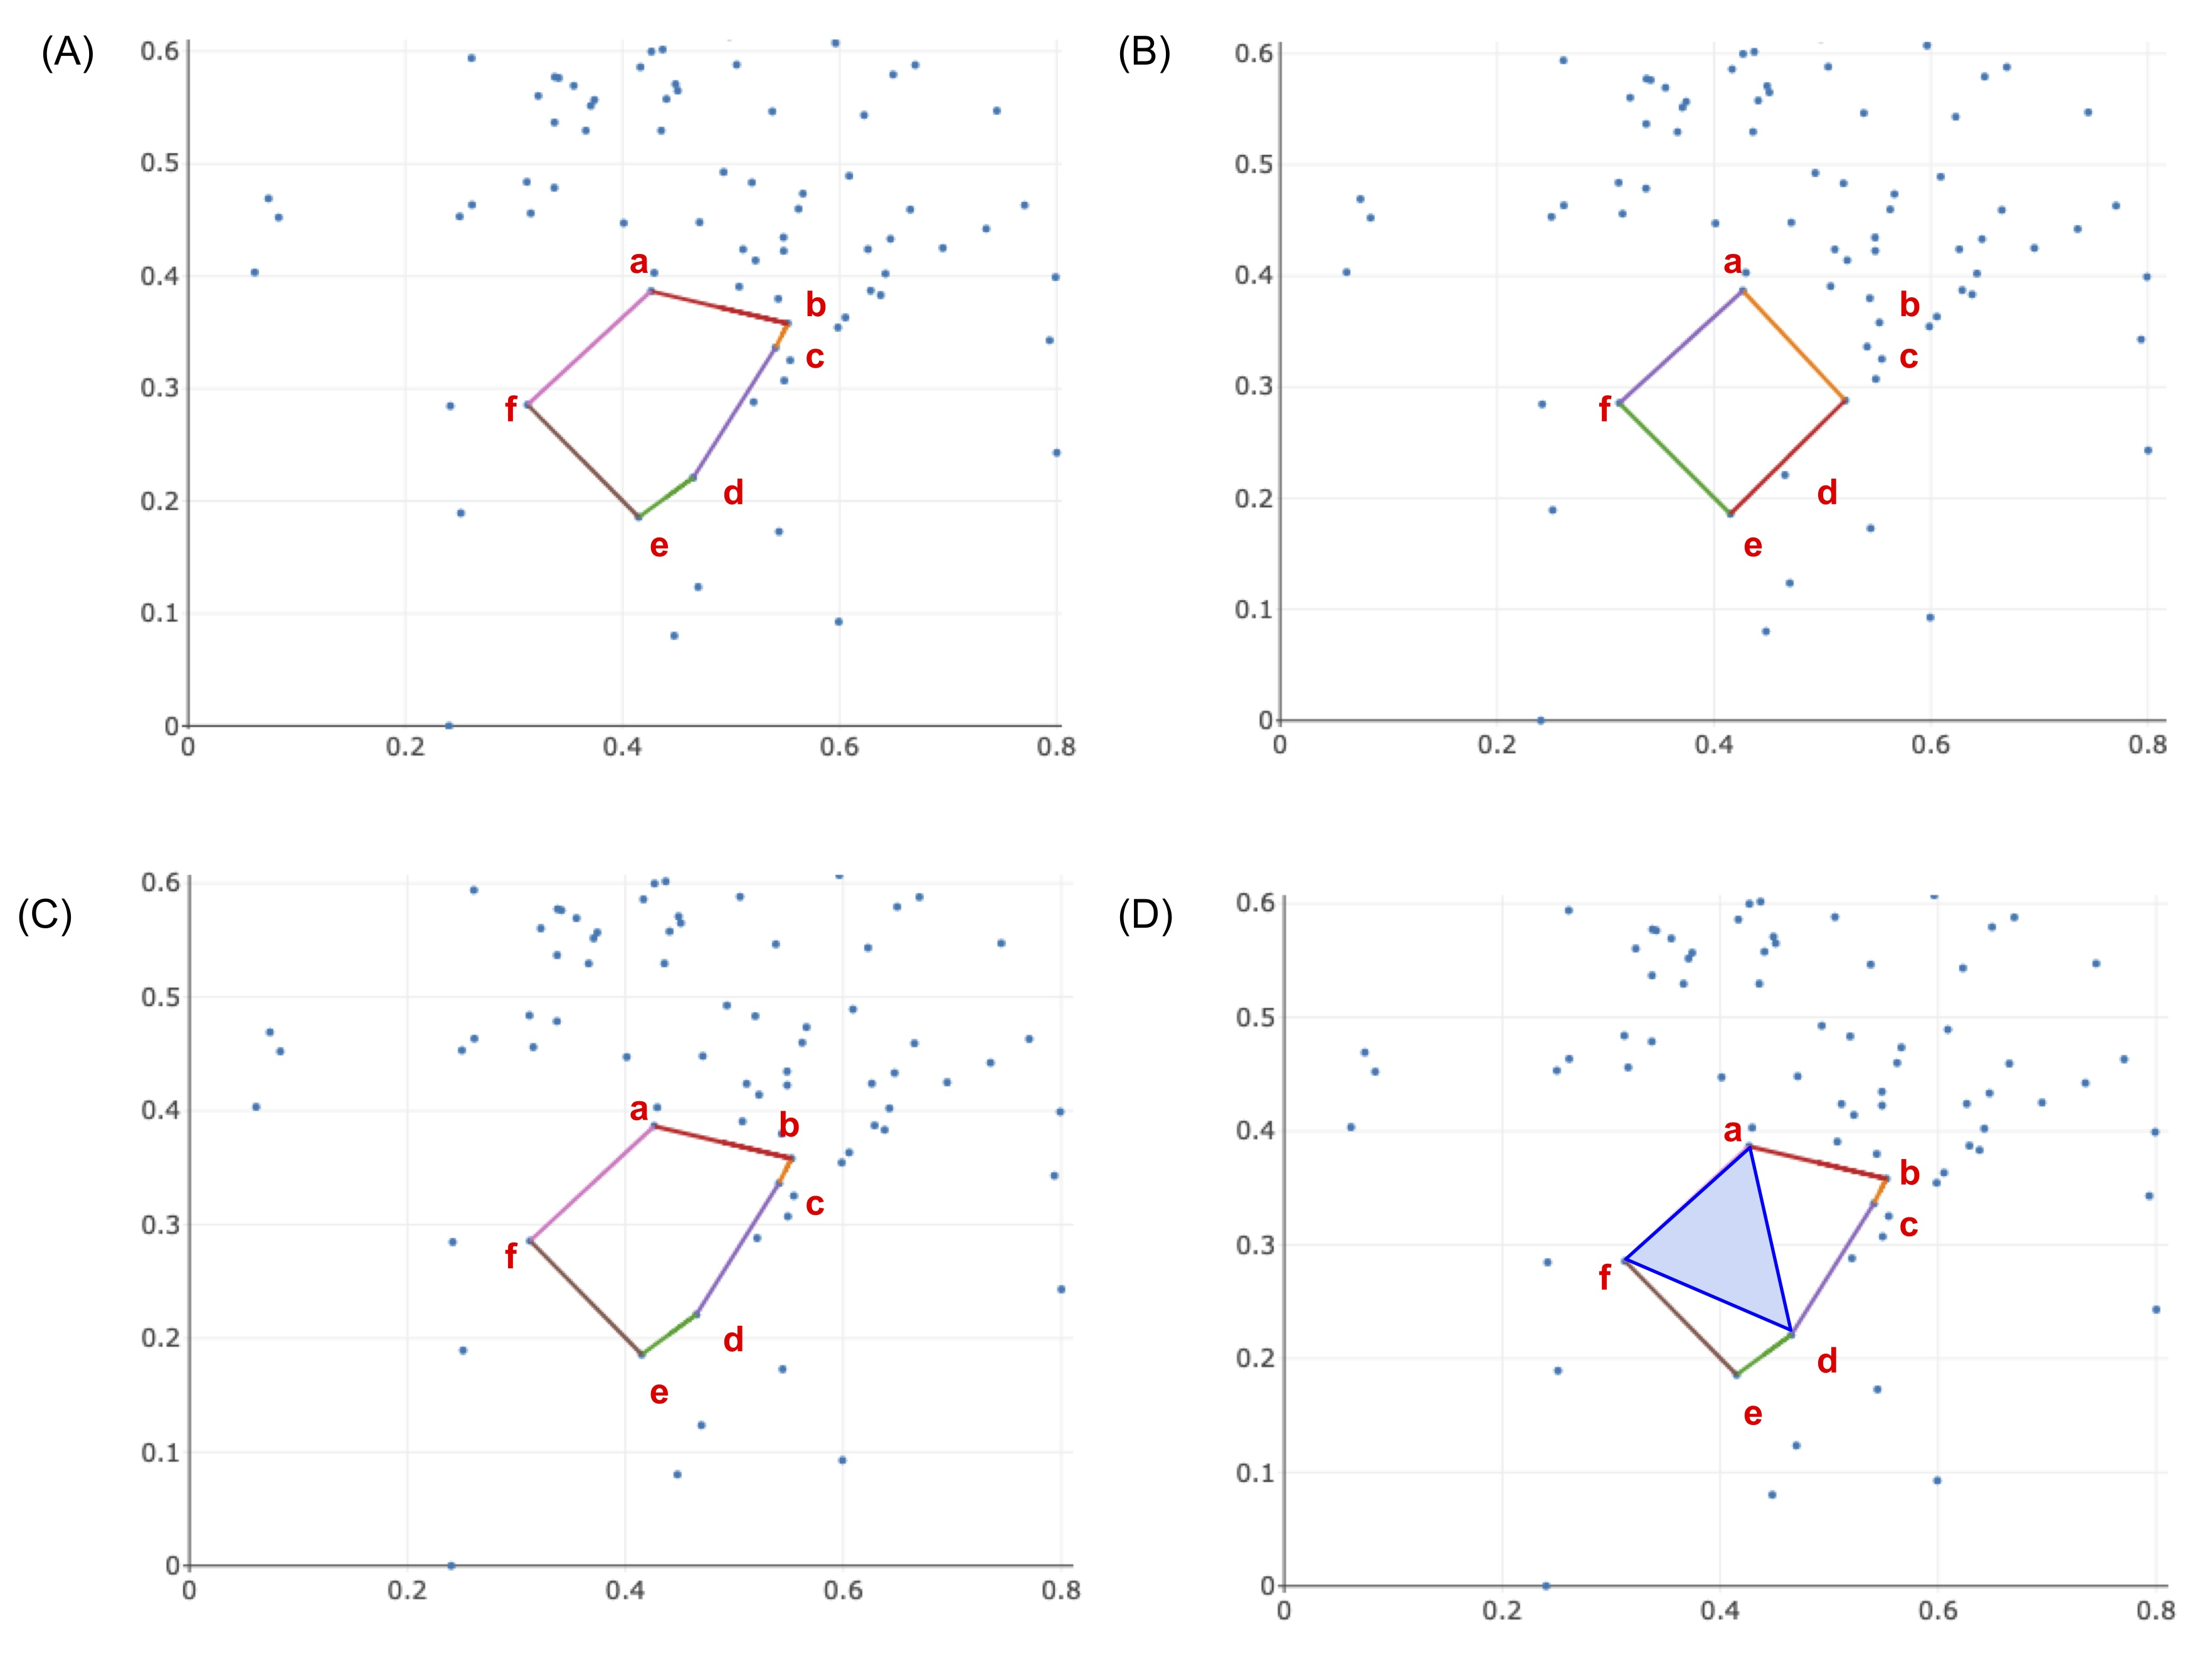
\includegraphics[width=15cm]{figures/areaexample.jpg}
\DIFaddendFL \end{center}
\caption{\DIFdelbeginFL \DIFdelFL{Number of loops in }\DIFdelendFL \DIFaddbeginFL \DIFaddFL{An example illustrating when }\DIFaddendFL the \DIFaddbeginFL \DIFaddFL{area enclosed by the triangle-loss area-weighted optimal cycle, solution to \pr \ref{itm:tri_NIA}, can be larger than the area enclosed by the edge-loss length-weighted minimal cycle, solution to \pr \ref{itm:edge_NIL}. }\textbf{\DIFaddFL{(A)}} \DIFaddFL{is the }\DIFaddendFL original cycle \DIFdelbeginFL \DIFdelFL{representatives }\DIFdelendFL of \DIFdelbeginFL \DIFdelFL{each dimension (subfigure title) }\DIFdelendFL \DIFaddbeginFL \DIFaddFL{a representative point cloud }\DIFaddendFL in \DIFaddbeginFL \DIFaddFL{$\mathbb{R}^2$ drawn from }\DIFaddendFL the \DIFdelbeginFL \DIFdelFL{$360$ randomly generated }\DIFdelendFL \DIFaddbeginFL \DIFaddFL{normal }\DIFaddendFL distribution\DIFdelbeginFL \DIFdelFL{data sets. The horizontal axis }\DIFdelendFL \DIFaddbeginFL \DIFaddFL{, }\textbf{\DIFaddFL{(B)}} \DIFaddendFL is the \DIFdelbeginFL \DIFdelFL{number of representatives and the vertical axis }\DIFdelendFL \DIFaddbeginFL \DIFaddFL{length-weighted edge-loss optimal cycle, }\textbf{\DIFaddFL{(C)}} \DIFaddendFL is the \DIFdelbeginFL \DIFdelFL{number of loops }\DIFdelendFL \DIFaddbeginFL \DIFaddFL{area-weighted triangle-loss optimal cycle, }\DIFaddendFL in \DIFaddbeginFL \DIFaddFL{this example, it is }\DIFaddendFL the \DIFaddbeginFL \DIFaddFL{same cycle as the }\DIFaddendFL original \DIFdelbeginFL \DIFdelFL{representative}\DIFdelendFL \DIFaddbeginFL \DIFaddFL{cycle, }\textbf{\DIFaddFL{(D)}} \DIFaddFL{is the area-weighted minimal cycle where the blue shaded area marks the triangle born at the death time of the cycle}\DIFaddendFL .  
\DIFdelbeginFL \DIFdelFL{We observe }\DIFdelendFL \DIFaddbeginFL \DIFaddFL{Constraint Equation \ref{obacond1} specifies }\DIFaddendFL that \DIFdelbeginFL \DIFdelFL{original }\DIFdelendFL \DIFaddbeginFL \DIFaddFL{the area-weighted optimal }\DIFaddendFL cycle \DIFdelbeginFL \DIFdelFL{representatives can }\DIFdelendFL \DIFaddbeginFL \DIFaddFL{must contain the 2-simplex born at the death time of the cycle. Therefore, this cycle must contain $\{a,d,f\}$ because it was born at the death time. The length-weighted minimal cycle does not }\DIFaddendFL have \DIFdelbeginFL \DIFdelFL{up to 10 loops in higher dimensions}\DIFdelendFL \DIFaddbeginFL \DIFaddFL{this constraint}\DIFaddendFL , and \DIFdelbeginFL \DIFdelFL{in general}\DIFdelendFL \DIFaddbeginFL \DIFaddFL{as such}\DIFaddendFL , \DIFdelbeginFL \DIFdelFL{it is not uncommon to find an original representative with multiple loops}\DIFdelendFL \DIFaddbeginFL \DIFaddFL{can result in a smaller area}\DIFaddendFL . 
}\DIFaddbeginFL \label{fig:areaExample}
\end{figure}


 \begin{figure}[h!]
\begin{center}
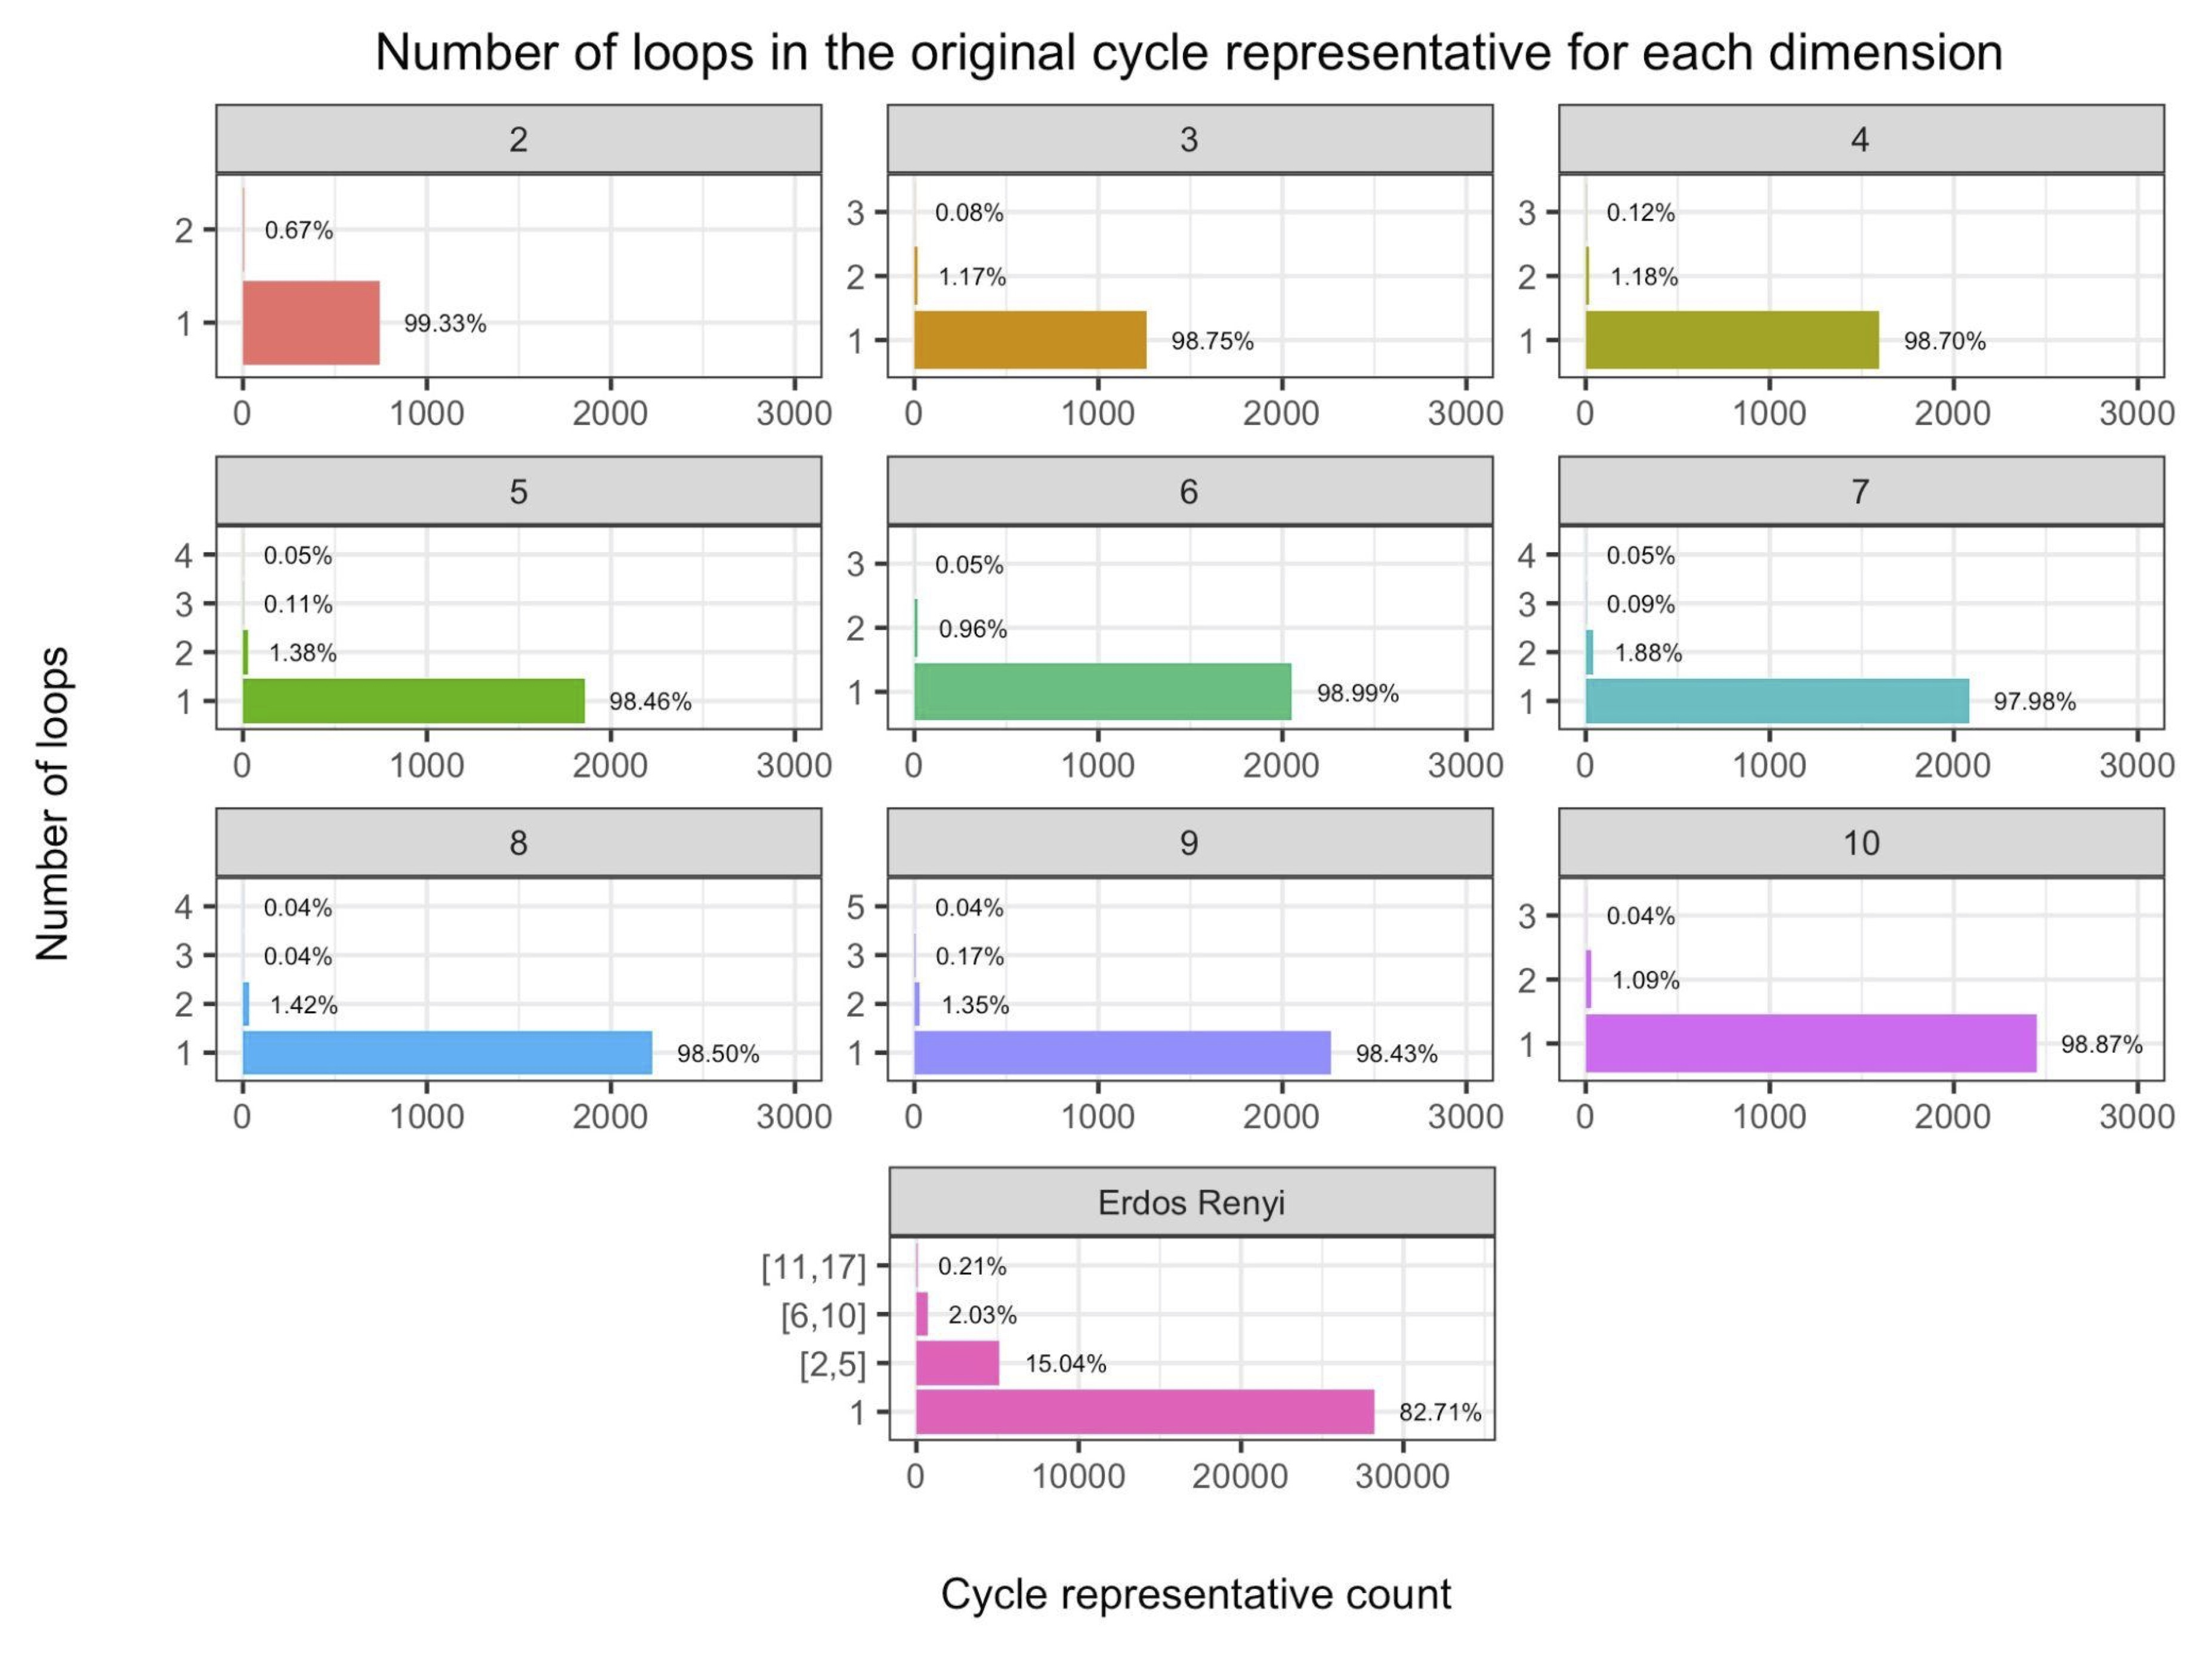
\includegraphics[width=\textwidth]{figures/loopsbreakdown.jpg}
\end{center}
\caption{  
\DIFaddFL{(Rows 1-3) Number of loops in the original cycle representative aggregated by dimension (labeled by subfigure title) in the  $360$ randomly generated distribution data sets discussed in Section \ref{sec: randompointclouds} and (Row 4) same for the  Erd\H{o}s-R\'enyi random complexes discussed in Section \ref{sec:erdos}, where we bin cycle representatives that have 2-5 loops, 6-10, loops, or more than 10 loops. The horizontal axis is the number of cycle representatives and the vertical axis is the number of loops in the original representative. We observe that for the distribution data, an original cycle representative can have up to 5 loops in higher dimensions, and in general, it is uncommon to find an original representative with multiple loops. However, we observe that $17.47\%$ of the cycle representatives for Erd\H{o}s-R\'enyi complexes have more than $1$ loop, with a maximum number of $17$ loops in a cycle representative.}}
\DIFaddendFL \label{fig:loopsbreakdown}
\end{figure} 

\newpage 
\begin{figure}[h!]
\begin{center}
\DIFdelbeginFL %DIFDELCMD < 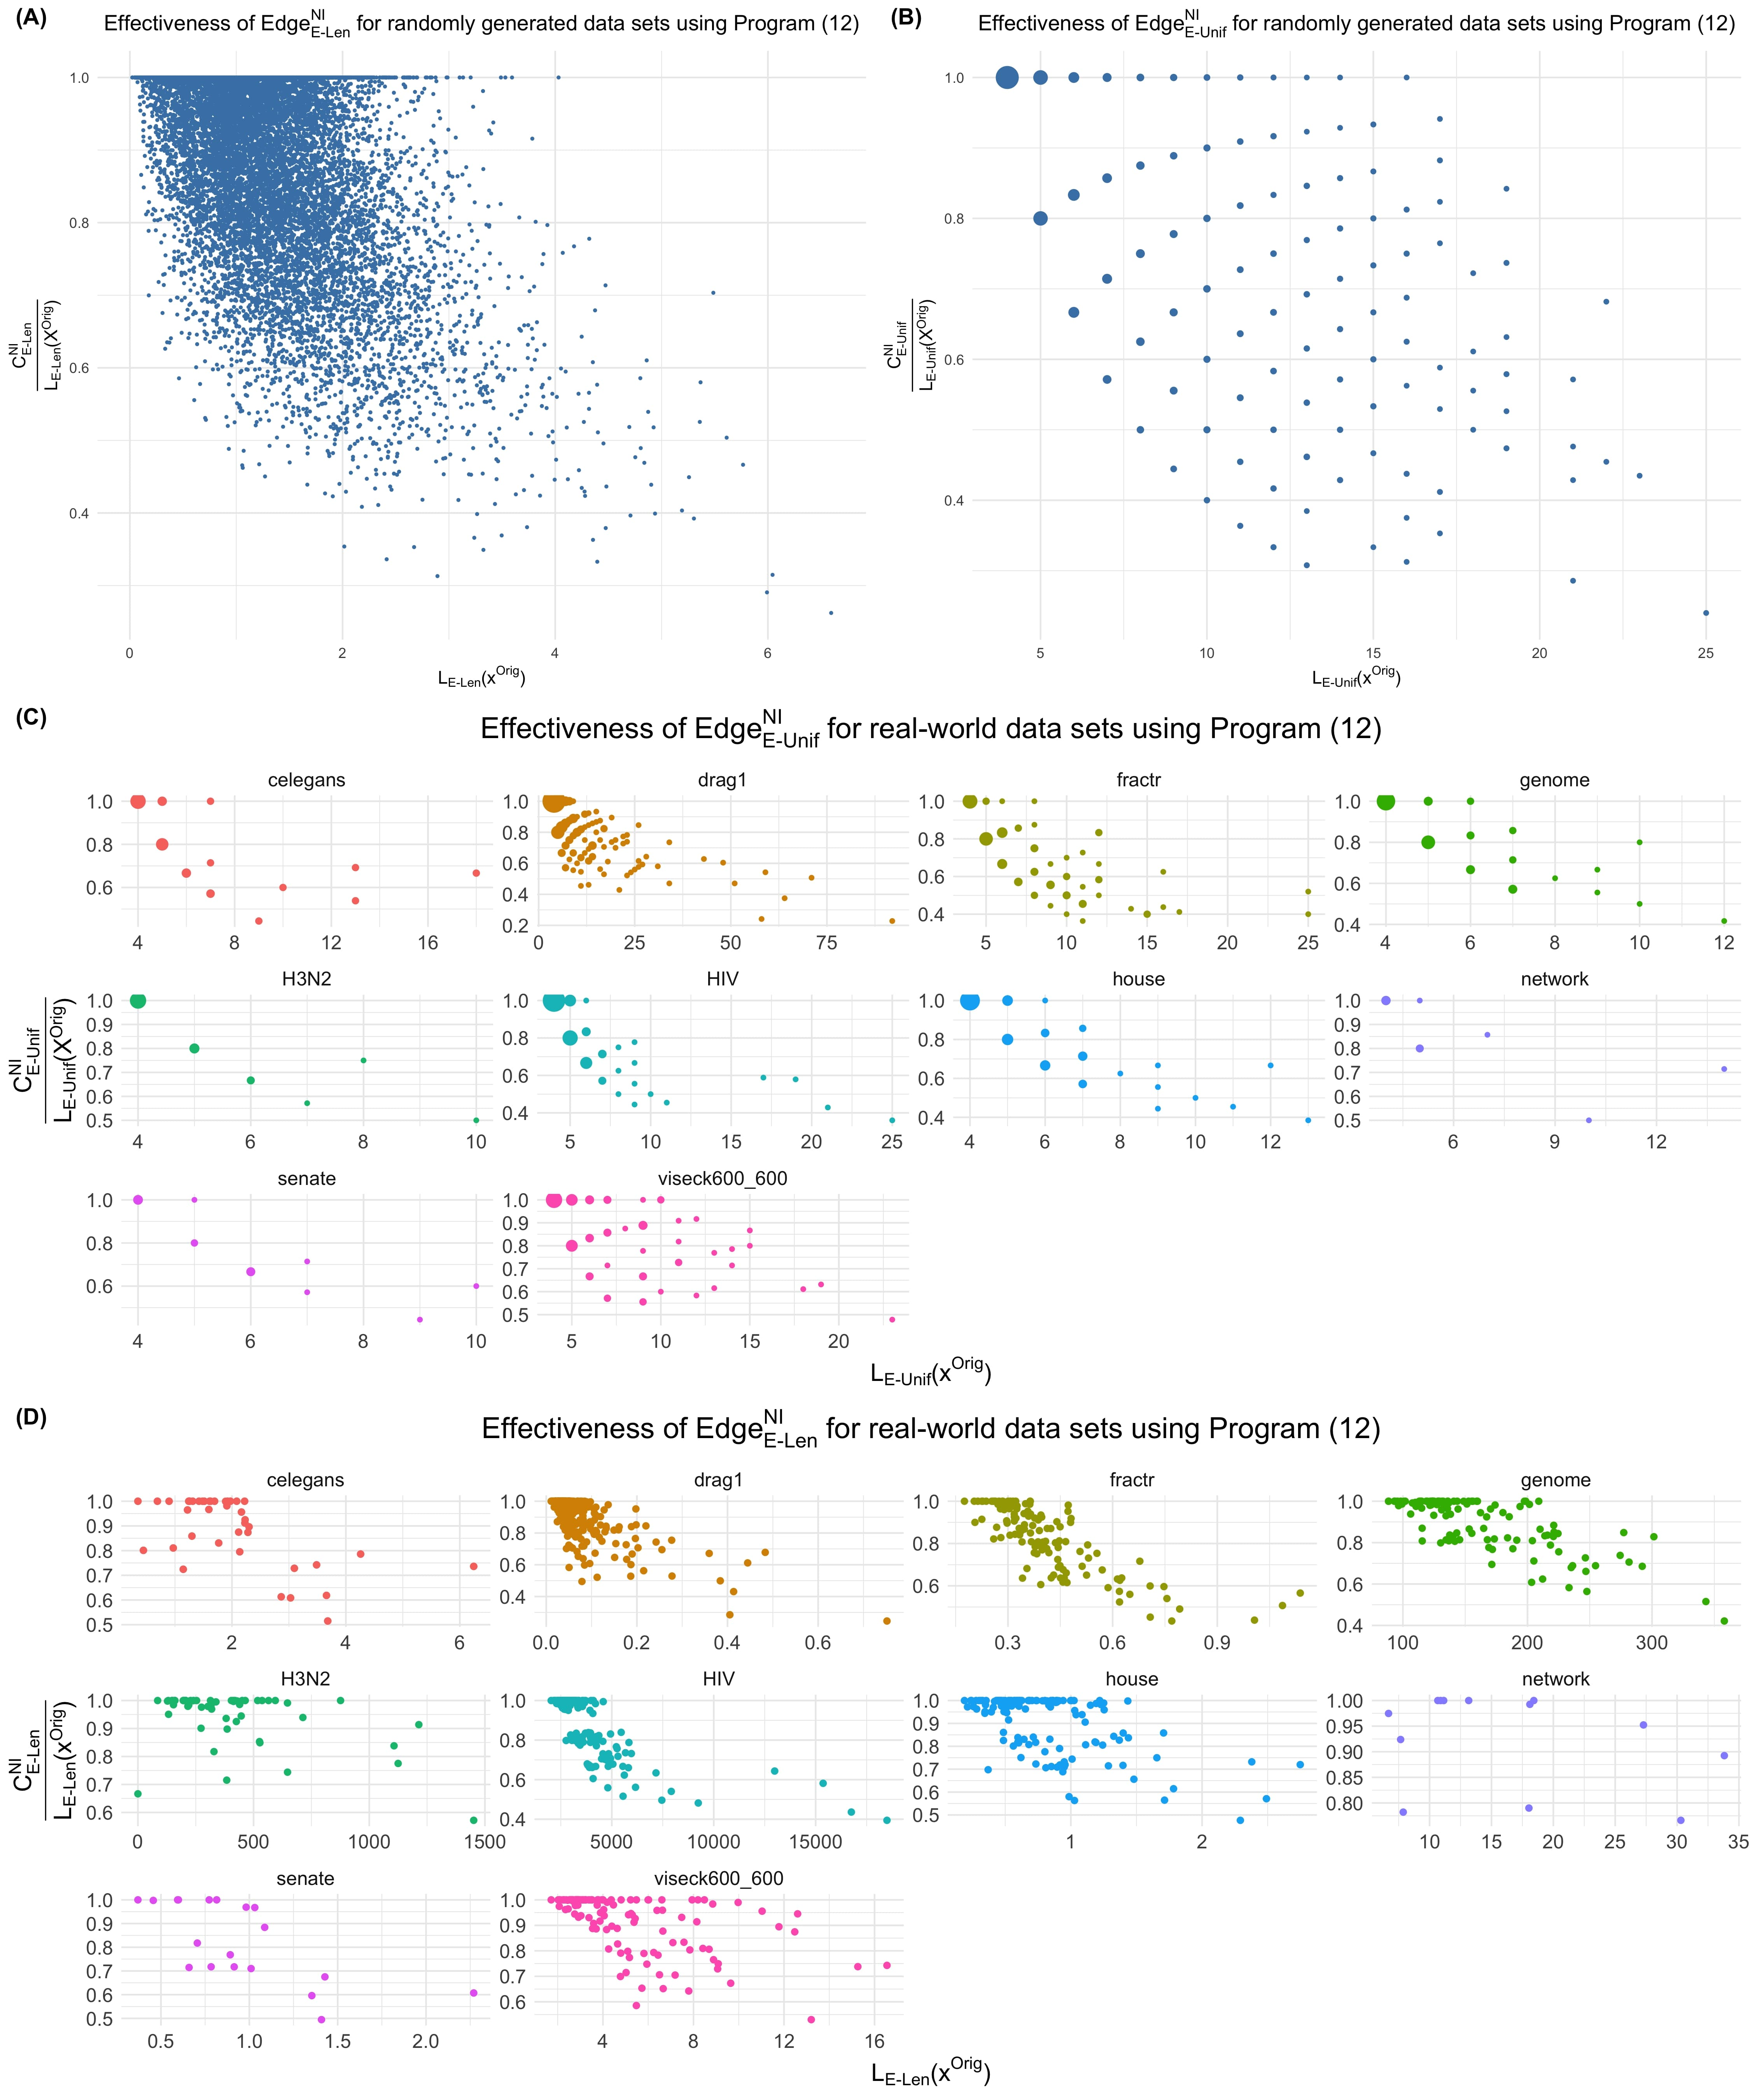
\includegraphics[width=0.95\textwidth]{figures/four_eff_df2.jpg} 
%DIFDELCMD < %%%
\DIFdelendFL \DIFaddbeginFL 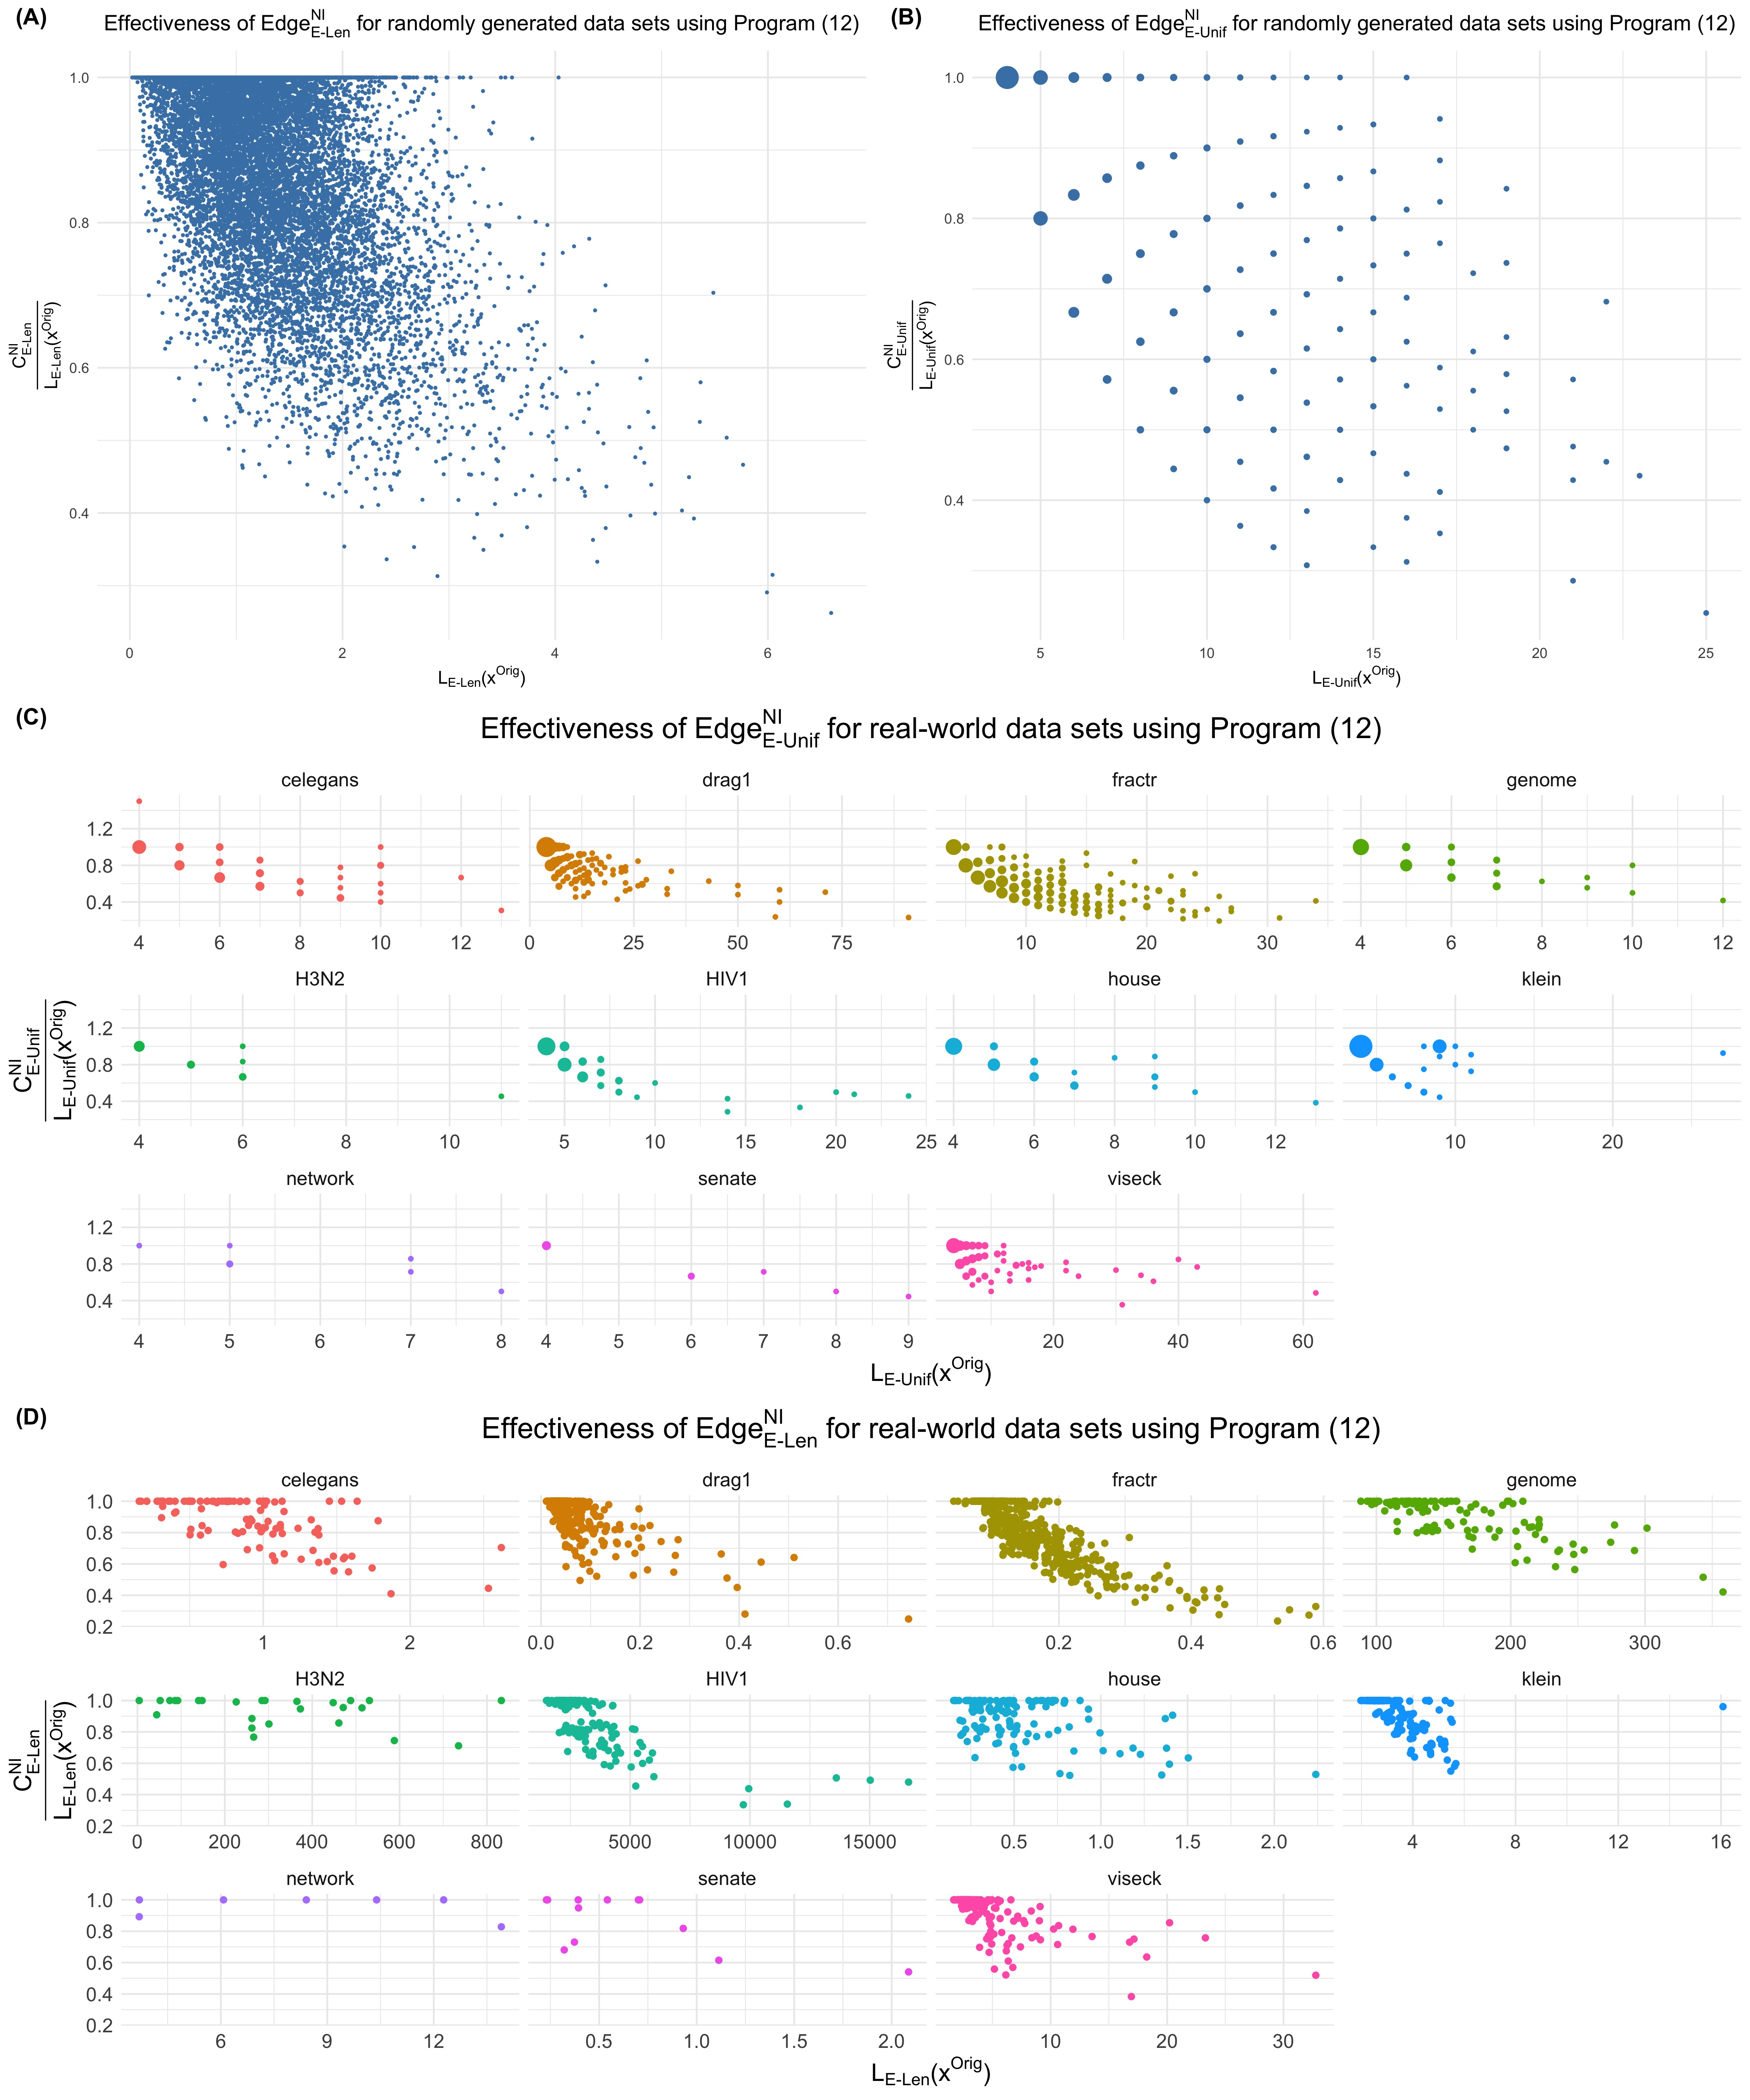
\includegraphics[width=0.95\textwidth]{figures/four_eff_df.jpg} 
\DIFaddendFL \end{center}
\caption{The effectiveness of length-weighted and uniform-weighted optimization for the \DIFdelbeginFL \DIFdelFL{randomly generated }\DIFdelendFL data sets \DIFaddbeginFL \DIFaddFL{in Sections \ref{sec: realworlddata} }\DIFaddendFL and \DIFdelbeginFL \DIFdelFL{real-world data sets }\DIFdelendFL \DIFaddbeginFL \DIFaddFL{\ref{sec: randompointclouds} }\DIFaddendFL in reducing the size of the original cycle representative found by the persistence algorithm. In each subfigure, the horizontal axis is the size of the original representative and the vertical axis is the ratio between the size of the optimal representative and the size of the original representative. The uniform-weighted graphs appear more sparse because reductions in the cost $L_{T\text{-}Unif}(\originalrep)$ can only come in multiples of the reciprocal of the original length. The node size in the \DIFdelbeginFL \DIFdelFL{uniform-weighed }\DIFdelendFL \DIFaddbeginFL \DIFaddFL{uniform-weighted }\DIFaddendFL graphs corresponds to the number of overlapping points. %DIF > One of the generators for the Celegans data set has a generator with 0.5 entries. 
}\label{fig:effectivenessall} 
\end{figure}

\newpage 
 \begin{figure}[h!]
\begin{center}
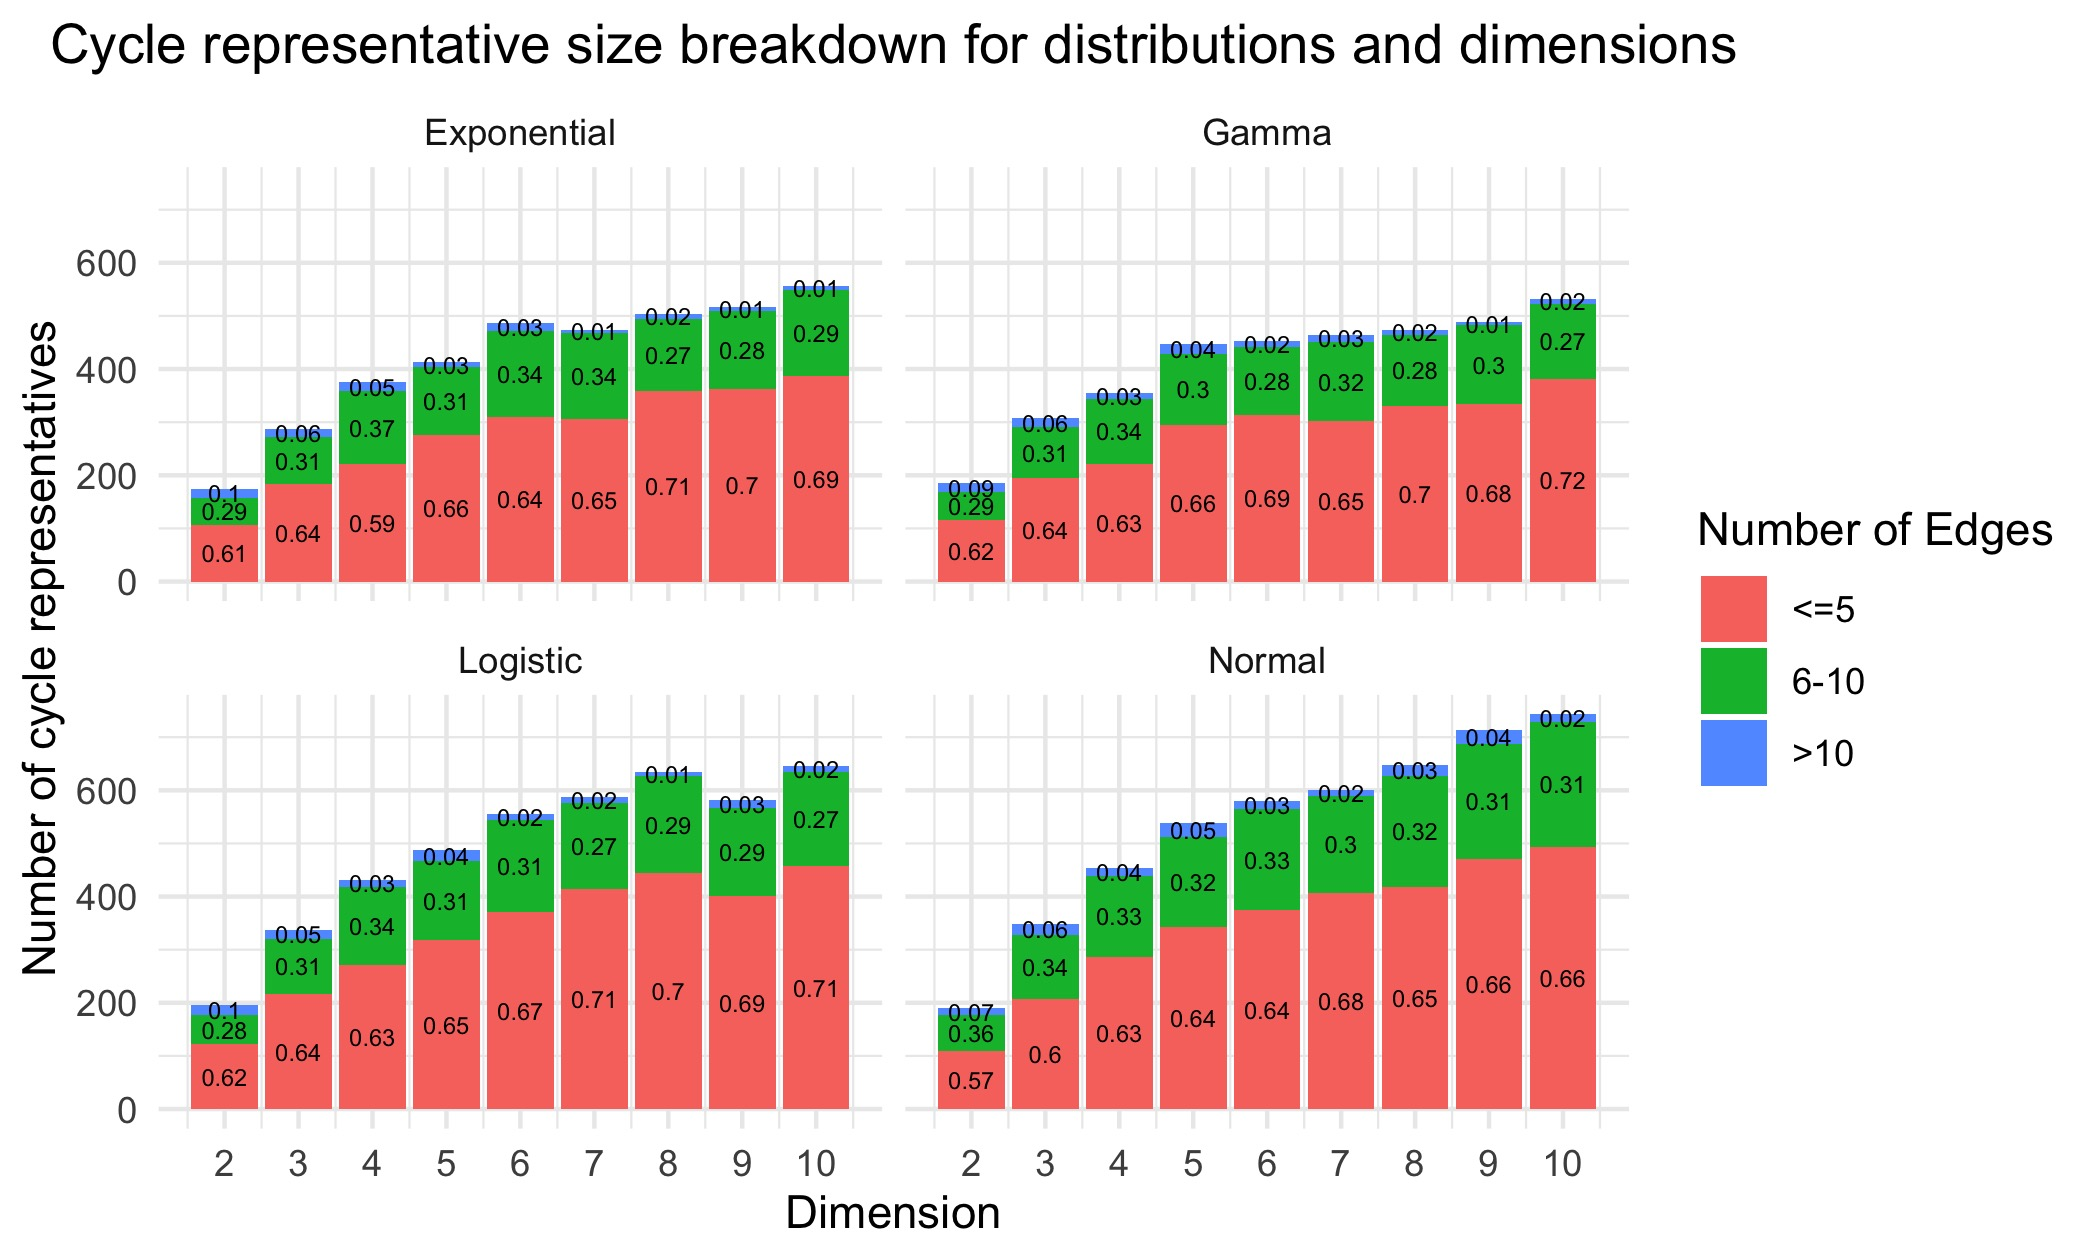
\includegraphics[width=1\textwidth]{figures/generator_breakdown.jpg} 
\end{center}
\caption{The number of original cycle representatives and the number of edges within each original representative for data described in \se \ref{sec: randompointclouds}. These plots aggregate all cycle representatives for each dimension of a particular distribution. The horizontal axis for each subplot is the dimension of the data set, and the vertical axis is the number of cycle representatives found in each dimension. In general, we see there are more cycle representatives in higher dimensional data sets. Each bar is partitioned by the number of edges of the representative. We observe that as dimension increases, there tend to be more cycle representatives with more edges. 
}\label{fig:gen_num_breakdown}
\end{figure}

\DIFdelbegin %DIFDELCMD < \newpage 
%DIFDELCMD <  %%%
\DIFdelend \DIFaddbegin \begin{figure}
    \centering
    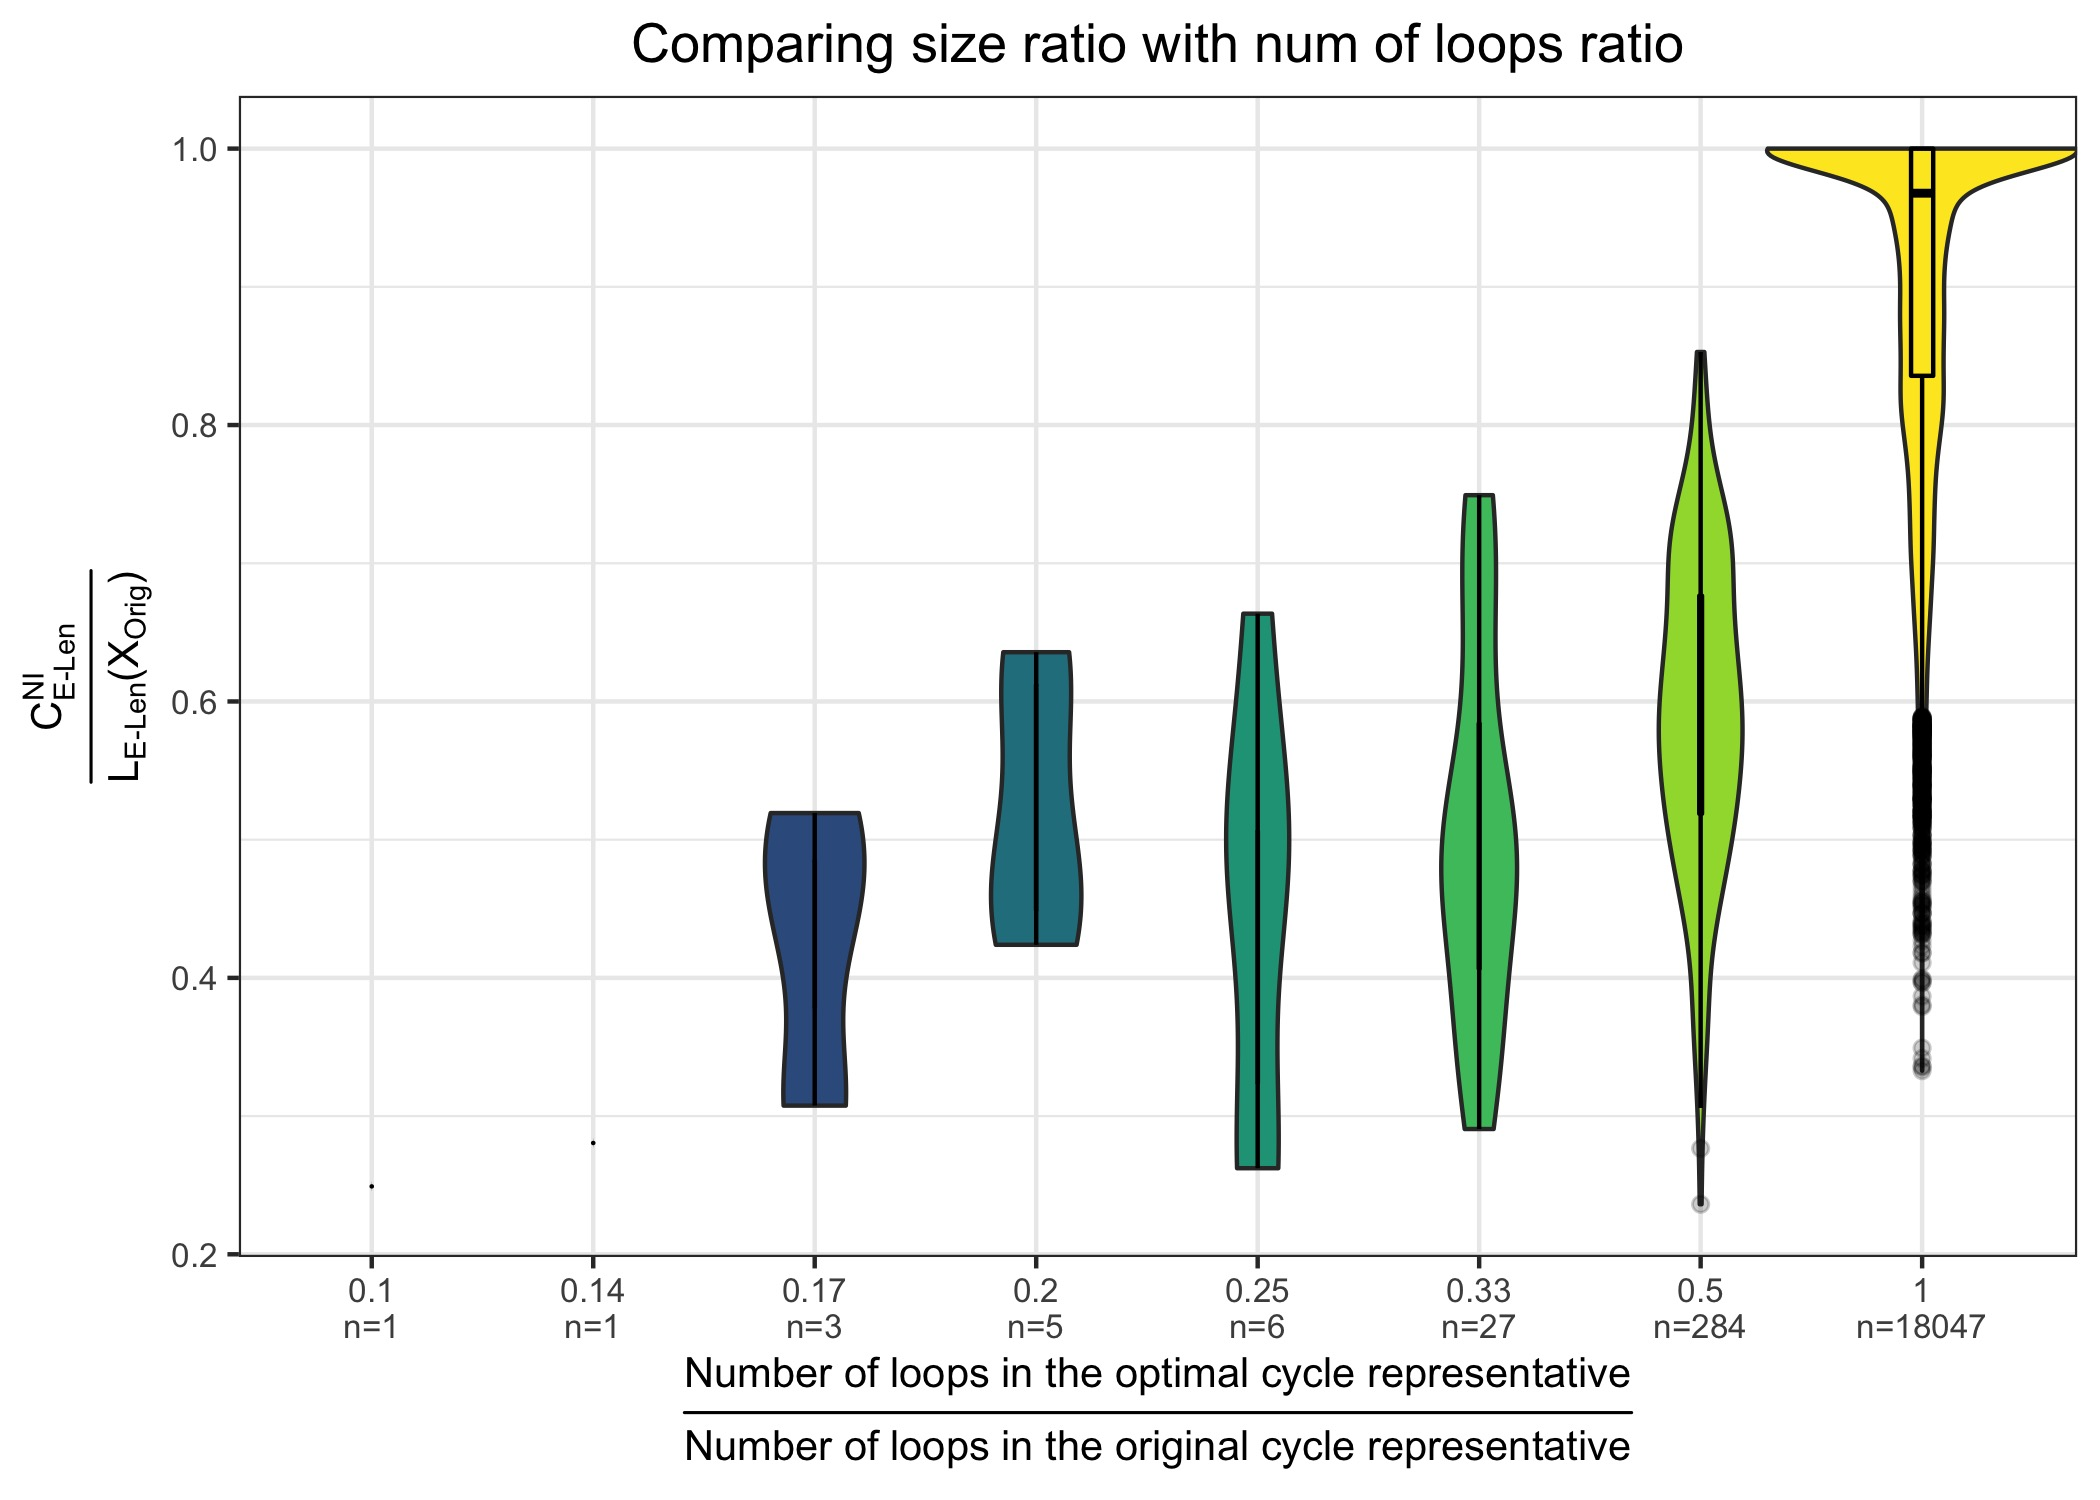
\includegraphics[width=0.9\textwidth]{figures/sizeratio_loopratio.jpg}
    \caption{\DIFaddFL{Violin plot of the effectiveness of the optimization as a function of the number of loops in the original cycle representative.  Results are aggregated over the data sets from \se \ref{sec: realworlddata} and \ref{sec: randompointclouds}. The $x$-axis shows the size reduction in terms of number of loops, and the $y$-axis shows the size reduction in terms of the length of the cycle. We can see that in general, the reduction in size of the original cycle mostly comes from the reduction in the number of loops by the optimization. }} 
    \label{fig:my_label}
\end{figure}
\DIFaddend 

%DIF >  \newpage 
%DIF >  \begin{table}[!h]
%DIF >  \caption{distmat}
%DIF >      {\footnotesize{
%DIF >      \begin{tabular}{ |>{\centering}m{11em} *{11}{>{\centering\arraybackslash}m{4.5em} }|}
%DIF >   \hline
%DIF >    & \textbf{Klein} & \textbf{Vicsek}  & \textbf{C.elegans} & \textbf{HIV} & \textbf{Genome}  & \textbf{fractal R} & \textbf{network} & \textbf{house} & \textbf{senate} & \textbf{drag} & \textbf{H3N2}\\[0.5ex] 
%DIF >   \hline 
%DIF >   \hline
%DIF >   \textbf{Ambient dimension} & 3 & 3 & 202 &  673 & 688 &  259 & 300 & 261 & 60 & 3 &  1,173\\   
%DIF >   \textbf{\# points}   & 400 &  300  &  297 &   1088 &  1397  & 512 & 379 & 445  & 103 & 1,000 & 2,722\\ 
%DIF >   \textbf{\# representatives}& 257  & 124  &  107 &174   &  117 (115)   & 438 & 7  & 126  & 12 & 311 & 28 (26) \\  
%DIF >   \textbf{$T$ persistence}   & 100.97  & 6.81 & 5.14 &728.51& 967.61     & 143.07 & 12.18  &  9.62 & 0.10 & 1,053.53 & 71,081.77  \\ 
%DIF >   [0.5ex] 
%DIF >  \hline
%DIF >  \multicolumn{5}{c}{\textbf{\qquad Edge-loss persistent homological cycle representatives (\pr \eqref{eq:edgelossgeneral})}} &&&&&& \\
%DIF >  \hline
%DIF >  %  \textbf{Memory (GiB)}    & 5.56 & 3.05 & 199.52 & 181.27  & 7.71 & 72.17 & 7.16 & 0.15& 416.38\\ \hline        
%DIF >   \textbf{$T\I_{E\text{-}Len}$ optimization} & 16.01  & 8.2 &  19.64&466.85  &     & 150.46 & 0.17 & 63.93  & 0.31 & 45.14 & 4,732.59	\\ 
%DIF >   \textbf{$T\NI_{E\text{-}Len}$ optimization} & 11.28  & 6.61 &16.07  &403.63 &     & 86.95 & 0.13 & 48.65  & 0.22 & 34.73 & 4,540.55 \\ 
%DIF >   \textbf{$T\I_{E\text{-}Unif}$ optimization} & 14.59  & 9.09 & 19.22 & 473.82 &     & 119.94 & 0.23 &  63.34 & 0.33 & 45.51 & 4,714.90	\\ 
%DIF >    \textbf{$T\NI_{E\text{-}Unif}$ optimization} & 11.38  & 5.55 & 15.63 & 404.95 &     & 83.40 & 0.12 & 48.88  & 0.22 & 33.88 & 4,547.37 \\
%DIF >    [0.5ex] 
%DIF >  \hline
%DIF >  \multicolumn{5}{c}{\textbf{Edge-loss filtered homological cycle represnetatives (\pr \eqref{eq:escolarargmin})}} &&&&&& \\
%DIF >  \hline
%DIF >  %  \textbf{Memory (GiB)}    & 5.56 & 3.05 & 199.52 & 181.27  & 7.71 & 72.17 & 7.16 & 0.15& 416.38\\ \hline        
%DIF >   \textbf{$T\I_{E\text{-}Len}$ optimization} & 16.93  &8.64  &20.41  & 468.22 &     &  155.08&  0.17 &  62.20  & 0.30 & 67.77 & 2,999.24	\\ 
%DIF >   \textbf{$T\NI_{E\text{-}Len}$ optimization} & 10.29  & 5.51 &16.15  & 403.74 &     & 88.66 &0.13  &  48.24 & 0.22 & 50.25 & 2,829.12	\\ 
%DIF >   \textbf{$T\I_{E\text{-}Unif}$ optimization} & 15.14  & 8.32 &19.76  & 476.84  &     &  142.4&  0.24  & 61.82  & 0.31 & 68.63 & 2,937.16	\\ 
%DIF >    \textbf{$T\NI_{E\text{-}Unif}$ optimization} & 11.07  & 5.63 & 16.23 & 406.97 &     & 87.59 &  0.12 & 48.11  &0.22  & 54.05 & 2,833.06	 \\
%DIF >    [0.5ex] 
%DIF >  \hline
%DIF >  \multicolumn{5}{c}{\textbf{Triangle-loss persistent homological cycle representatives (\pr \eqref{eq:trianglelossgeneral})\qquad}} &&&&&& \\
%DIF >  \hline
%DIF >   \textbf{$T\I_{T\text{-}Unif}$ optimization} & 423.32 & 23.07  &783.06  & 63,227.14 &  &  10,187.41   & 2.71 & 221.07  & 0.26  & 384.91 & 39,140.67 \\ 
%DIF >   \textbf{$T\NI_{T\text{-}Unif}$ optimization} & 287.49 & 18.81 & 610.20 &60,459.49 &  &   8,441.76  & 2.08 & 170.95  & 0.23  & 277.93 & 36,401.50  \\ 
%DIF >   \textbf{$T$ build all}  & 5.52  & 0.88  & 10.07 & 826.25 &  & 45.28 & 0.05 &  4.85 & 0.03  & 172.60 & - \\ 
%DIF >  \textbf{Total $T$ build part}  & 6.13 & 3.06  &24.21 & 860.91 &  & 193.99 & 0.26 & 31.37  & 0.03  & 198.27 & 922.50 \\ \hline 
%DIF >  \end{tabular}
%DIF >  }%\LL{Updated 03/14}
%DIF >  }
%DIF >  \label{tab:realworldata}
%DIF >  \end{table}
 \DIFaddbegin 

\DIFaddend \begin{table}[!h]
\caption{Summary of the experimental results of the data sets from \cite{roadmap2017} as described in \se \ref{sec: realworlddata}. The rows include the ambient dimension, number of points, the number of cycle representatives in $\Homologies_1$, and the time (measured in seconds) it took to compute persistent homology for each data set. We also include the computation time taken to optimize the set of cycle representatives under six different optimization problems, and computation time of two different implementation choices for the triangle-loss optimal cycles: building the full $\partial_2$ boundary matrix once and extracting the part needed, or constructing part of the $\partial_2$ boundary matrix for each cycle representative. In this table, $T$ stands for computation time measured in seconds with subscripts indicating the type of the optimal cycle and superscripts indicating whether the program was solved using linear programming (NI) or integer programming (I). The time taken to construct the input to the optimization problem is included in the optimization time for edge-loss minimal cycle representatives, but is excluded and separately listed in the last two rows for the triangle-loss minimal cycle representatives. For triangle-loss cycles, we were able to compute $115$ out of the $117$ cycle representatives for the \textbf{Genome} data set and $52$ out of $57$ cycle representatives for the \textbf{H3N2} data set due to memory constraints. The numbers in the parenthesis represent the other optimization statistics corresponding to the triangle-loss optimal cycles we were actually able to compute. The last two rows compare two ways of building the input $\partial_2[:,\hat {\mathcal{F}}_{2}]$ matrix to the triangle-loss optimal cycle program. The penultimate row records the time of building the entire $\partial_{2}$ matrix once and then extracting columns born in the interval $\closedinterval$ for each representative. The last row records the total time to iteratively build the part of the boundary matrix $\partial_2[:,\hat {\mathcal{F}}_{2}]$ for each cycle representative.}
    {\DIFdelbeginFL %DIFDELCMD < \footnotesize{ 
%DIFDELCMD <     \begin{tabular}{ |>{\centering}m{11em} *{11}{>{\centering\arraybackslash}m{4.5em} }|}
%DIFDELCMD <  \hline
%DIFDELCMD <   & \textbf{Klein} & \textbf{Vicsek}  & \textbf{C.elegans} & \textbf{HIV} & \textbf{Genome}  & \textbf{fractal R} & \textbf{network} & \textbf{house} & \textbf{senate} & \textbf{drag} & \textbf{H3N2}\\[0.5ex] 
%DIFDELCMD <  \hline 
%DIFDELCMD <  \hline
%DIFDELCMD <  \textbf{Ambient dimension} & 3 & 3    & 202 &  673 & 688 &  259 & 300 & 261 & 60 & 3 &  1,173\\   
%DIFDELCMD <  \textbf{\# points}   & 400 &  300  &  297 &   1088 &  1397  & 512 & 379 & 445  & 103 & 1,000 & 2,722\\ 
%DIFDELCMD <  \textbf{\# representatives} & 257 & 124  &42& 199& 117 (115) & 126&  13 & 133 & 19& 311 & 57 (53) \\  
%DIFDELCMD <  \textbf{$T$ persistence} &   66.21  & 5.48  & 3.41 & 552.80 &  967.61  & 62.99 & 10.23 & 7.79 & 0.12 & 948.16 & 23,362.05 \\ 
%DIFDELCMD <  [0.5ex] 
%DIFDELCMD < \hline
%DIFDELCMD < \multicolumn{5}{c}{\textbf{\qquad Edge-loss persistent homological cycle representatives (\pr \eqref{eq:edgelossgeneral})}} &&&&&& \\
%DIFDELCMD < \hline        
%DIFDELCMD <  \textbf{$T\I_{E\text{-}Len}$ optimization} & 16.01 & 8.24 & 13.22 & 957.48 & 656.05 & 78.1 & 0.72 & 66.23 & 0.38 & 45.14 &5469.85	\\ 
%DIFDELCMD <  \textbf{$T\NI_{E\text{-}Len}$ optimization} & 11.28 & 5.66 & 9.94 & 850.09 & 491.69 & 53.85 & 0.57 & 48.53 & 0.29 & 34.73 &4989.13	\\ 
%DIFDELCMD <  \textbf{$T\I_{E\text{-}Unif}$ optimization} & 14.59 & 8.66 & 13.36 & 980.82 & 689.51 & 82.17 & 0.76 & 66.67 & 0.4 & 45.51 & 5274.77	\\ 
%DIFDELCMD <   \textbf{$T\NI_{E\text{-}Unif}$ optimization} & 11.38 & 5.66 & 10.39 & 872.12 & 492.66 & 54.96 & 0.56 & 49.72 & 0.31 & 33.88 & 4991.39	\\
%DIFDELCMD <   [0.5ex] 
%DIFDELCMD < \hline
%DIFDELCMD < \multicolumn{5}{c}{\textbf{Edge-loss filtered homological cycle represnetatives (\pr \eqref{eq:escolarargmin})}} &&&&&& \\
%DIFDELCMD < \hline       
%DIFDELCMD <  \textbf{$T\I_{E\text{-}Len}$ optimization} & 16.93 & 8.05 & 13.88 & 557.47 & 1144.17 & 75.56 & 0.97 & 61.84 & 0.35 & 67.77 & 5464.05	\\ 
%DIFDELCMD <  \textbf{$T\NI_{E\text{-}Len}$ optimization} & 10.29 & 6.15 & 11.3 & 464.34 & 973.15 & 53.86 & 0.66 & 43.22 & 0.26 & 50.25 & 4992.40	\\ 
%DIFDELCMD <  \textbf{$T\I_{E\text{-}Unif}$ optimization} & 15.14 & 8.53 & 13.2 & 562.57 & 1191.44 & 79.31 & 0.68 & 61.42 & 0.35 & 68.63 & 5277.85	\\ 
%DIFDELCMD <   \textbf{$T\NI_{E\text{-}Unif}$ optimization} & 11.07 & 5.94 & 10.35 & 467.22 & 981.72 & 53.86 & 0.53 & 43.66 & 0.43 & 54.05 &4988.87	 \\
%DIFDELCMD <   [0.5ex] 
%DIFDELCMD < \hline
%DIFDELCMD < \multicolumn{5}{c}{\textbf{Triangle-loss persistent homological cycle representatives (\pr \eqref{eq:trianglelossgeneral})\qquad}} &&&&&& \\
%DIFDELCMD < \hline
%DIFDELCMD <  \textbf{$T\I_{T\text{-}Unif}$ optimization} &   185.92 &72.69 &  477.53 &  21,072.34  & 16,379.86&  5,300.92 &     25.33  & 421.45 &    0.91 &  384.91 & 12,341.58\\ 
%DIFDELCMD <  \textbf{$T\NI_{T\text{-}Unif}$ optimization} & 103.26 & 62.42 & 372.46 & 18,958.53 & 14,535.42 & 4,411.80& 20.86  & 342.05 & 0.79 & 277.93 & 11,467.15\\ 
%DIFDELCMD <  \textbf{$T$ build all}  &5.52 & 3.56 &10.07 &  826.25& - & 47.8 & 12.55  & 6.82  &  0.08 & 172.60 & -\\ 
%DIFDELCMD < \textbf{Total $T$ build part} & 6.13  & 3.30 &   8.28 &  451.41 &415.79& 94.86 & 0.87 & 33.40 &  0.06  & 198.27 & 895.36\\ \hline 
%DIFDELCMD < \end{tabular}
%DIFDELCMD < } 
%DIFDELCMD < %%%
\DIFdelendFL \DIFaddbeginFL \footnotesize{ 
    \begin{tabular}{ |>{\centering}m{11em} *{11}{>{\centering\arraybackslash}m{4.5em} }|}
 \hline
  & \textbf{Klein} & \textbf{Vicsek}  & \textbf{C.elegans} & \textbf{HIV} & \textbf{genome} & \textbf{fractal R} & \textbf{network} & \textbf{house} & \textbf{senate} & \textbf{drag} & \textbf{H3N2}\\[0.5ex] 
 \hline 
 \hline
 \textbf{Ambient dimension} & 3 & 3 & 202 &  673  & 688 &  259 & 300 & 261 & 60 & 3 &  1,173\\   
 \textbf{\# points}   & 400 &  300  &  297 &   1088 &  1397    & 512 & 379 & 445  & 103 & 1,000 & 2,722\\ 
 \textbf{\# representatives}& 257  & 149  &  107 &174  &  117 (115)   & 438 & 7  & 126  & 12 & 311 & 28 (26) \\  
 \textbf{$T$ persistence}   & 100.97  & 129.39 & 5.14 &728.51  & 967.61  & 143.07 & 12.18  &  9.62 & 0.10 & 1,053.53 & 71,081.77  \\ 
 [0.5ex] 
\hline
\multicolumn{5}{c}{\textbf{\qquad Edge-loss persistent homological cycle representatives (\pr \ref{eq:edgelossgeneral})}}  &&&&&&& \\
\hline
%  \textbf{Memory (GiB)}    & 5.56 & 3.05 & 199.52 & 181.27  & 7.71 & 72.17 & 7.16 & 0.15& 416.38\\ \hline        
 \textbf{$T\I_{E\text{-}Len}$ optimization} & 16.01  & 8.2 &  19.64&466.85 & 656.05 &   150.46 & 0.17 & 63.93  & 0.31 & 45.14 & 4,732.59	\\ 
 \textbf{$T\NI_{E\text{-}Len}$ optimization} & 11.28  & 6.61 &16.07  &403.63 & 491.69  &    86.95 & 0.13 & 48.65  & 0.22 & 34.73 & 4,540.55 \\ 
 \textbf{$T\I_{E\text{-}Unif}$ optimization} & 14.59  & 9.09 & 19.22 & 473.82 & 689.51&    119.94 & 0.23 &  63.34 & 0.33 & 45.51 & 4,714.90	\\ 
  \textbf{$T\NI_{E\text{-}Unif}$ optimization} & 11.38  & 5.55 & 15.63 & 404.95& 492.66 & 83.40 & 0.12 & 48.88  & 0.22 & 33.88 & 4,547.37 \\
  [0.5ex] 
\hline
\multicolumn{5}{c}{\textbf{Edge-loss filtered homological cycle represnetatives (\pr \ref{eq:escolarargmin})}} &&&&&&& \\
\hline
%  \textbf{Memory (GiB)}    & 5.56 & 3.05 & 199.52 & 181.27  & 7.71 & 72.17 & 7.16 & 0.15& 416.38\\ \hline        
 \textbf{$T\I_{E\text{-}Len}$ optimization} & 16.93  &8.64  &20.41  & 468.22 & 1144.17 &    155.08&  0.17 &  62.20  & 0.30 & 67.77 & 2,999.24	\\ 
 \textbf{$T\NI_{E\text{-}Len}$ optimization} & 10.29  & 5.51 &16.15  & 403.74& 973.15 &     88.66 &0.13  &  48.24 & 0.22 & 50.25 & 2,829.12	\\ 
 \textbf{$T\I_{E\text{-}Unif}$ optimization} & 15.14  & 8.32 &19.76  & 476.84 & 1191.44 &     142.4&  0.24  & 61.82  & 0.31 & 68.63 & 2,937.16	\\ 
  \textbf{$T\NI_{E\text{-}Unif}$ optimization} & 11.07  & 5.63 & 16.23 & 406.97& 981.72  &    87.59 &  0.12 & 48.11  &0.22  & 54.05 & 2,833.06	 \\
  [0.5ex] 
\hline
\multicolumn{5}{c}{\textbf{Triangle-loss persistent homological cycle representatives (\pr \ref{eq:trianglelossgeneral})\qquad}} &&&&&&& \\
\hline
 \textbf{$T\I_{T\text{-}Unif}$ optimization} & 307.25 & 1496.01 &783.06  & 25,402.56  & 16,379.86  &  10,187.41   & 2.71 & 221.07  & 0.26  & 384.91 & 39,140.67 \\ 
  \textbf{$T\NI_{T\text{-}Unif}$ optimization} & 170.45 & 44.67 & 610.20 & 23,260.12  & 14,535.42  &   8,441.76  & 2.08 & 170.95  & 0.23  & 277.93 & 36,401.50  \\ 
 \textbf{$T$ build all}  & 1.45  & 0.32  & 10.07 & 268.57 & - &   45.28 & 0.05 &  4.85 & 0.03  & 172.60 & - \\ 
\textbf{Total $T$ build part}  & 8.80 & 3.51  &24.21 & 1,688.10 & 415.79&  193.99 & 0.26 & 31.37  & 0.03  & 198.27 & 922.50 \\ \hline 
\end{tabular}
%     \begin{tabular}{ |>{\centering}m{11em} *{11}{>{\centering\arraybackslash}m{4.5em} }|}
%  \hline
%   & \textbf{Klein} & \textbf{Vicsek}  & \textbf{C.elegans} & \textbf{HIV} & \textbf{Genome}  & \textbf{fractal R} & \textbf{network} & \textbf{house} & \textbf{senate} & \textbf{drag} & \textbf{H3N2}\\[0.5ex] 
%  \hline 
%  \hline
%  \textbf{Ambient dimension} & 3 & 3    & 202 &  673 & 688 &  259 & 300 & 261 & 60 & 3 &  1,173\\   
%  \textbf{\# points}   & 400 &  300  &  297 &   1088 &  1397  & 512 & 379 & 445  & 103 & 1,000 & 2,722\\ 
%  \textbf{\# representatives} & 257 & 124  &42& 199& 117 (115) & 126&  13 & 133 & 19& 311 & 57 (53) \\  
%  \textbf{$T$ persistence} &   66.21  & 5.48  & 3.41 & 552.80 &  967.61  & 62.99 & 10.23 & 7.79 & 0.12 & 948.16 & 23,362.05 \\ 
%  [0.5ex] 
% \hline
% \multicolumn{5}{c}{\textbf{\qquad Edge-loss persistent homological cycle representatives (\pr \eqref{eq:edgelossgeneral})}} &&&&&& \\
% \hline        
%  \textbf{$T\I_{E\text{-}Len}$ optimization} & 16.01 & 8.24 & 13.22 & 957.48 & 656.05 & 78.1 & 0.72 & 66.23 & 0.38 & 45.14 &5469.85	\\ 
%  \textbf{$T\NI_{E\text{-}Len}$ optimization} & 11.28 & 5.66 & 9.94 & 850.09 & 491.69 & 53.85 & 0.57 & 48.53 & 0.29 & 34.73 &4989.13	\\ 
%  \textbf{$T\I_{E\text{-}Unif}$ optimization} & 14.59 & 8.66 & 13.36 & 980.82 & 689.51 & 82.17 & 0.76 & 66.67 & 0.4 & 45.51 & 5274.77	\\ 
%   \textbf{$T\NI_{E\text{-}Unif}$ optimization} & 11.38 & 5.66 & 10.39 & 872.12 & 492.66 & 54.96 & 0.56 & 49.72 & 0.31 & 33.88 & 4991.39	\\
%   [0.5ex] 
% \hline
% \multicolumn{5}{c}{\textbf{Edge-loss filtered homological cycle represnetatives (\pr \eqref{eq:escolarargmin})}} &&&&&& \\
% \hline       
%  \textbf{$T\I_{E\text{-}Len}$ optimization} & 16.93 & 8.05 & 13.88 & 557.47 & 1144.17 & 75.56 & 0.97 & 61.84 & 0.35 & 67.77 & 5464.05	\\ 
%  \textbf{$T\NI_{E\text{-}Len}$ optimization} & 10.29 & 6.15 & 11.3 & 464.34 & 973.15 & 53.86 & 0.66 & 43.22 & 0.26 & 50.25 & 4992.40	\\ 
%  \textbf{$T\I_{E\text{-}Unif}$ optimization} & 15.14 & 8.53 & 13.2 & 562.57 & 1191.44 & 79.31 & 0.68 & 61.42 & 0.35 & 68.63 & 5277.85	\\ 
%   \textbf{$T\NI_{E\text{-}Unif}$ optimization} & 11.07 & 5.94 & 10.35 & 467.22 & 981.72 & 53.86 & 0.53 & 43.66 & 0.43 & 54.05 &4988.87	 \\
%   [0.5ex] 
% \hline
% \multicolumn{5}{c}{\textbf{Triangle-loss persistent homological cycle representatives (\pr \eqref{eq:trianglelossgeneral})\qquad}} &&&&&& \\
% \hline
%  \textbf{$T\I_{T\text{-}Unif}$ optimization} &   185.92 &72.69 &  477.53 &  21,072.34  & 16,379.86&  5,300.92 &     25.33  & 421.45 &    0.91 &  384.91 & 12,341.58\\ 
%  \textbf{$T\NI_{T\text{-}Unif}$ optimization} & 103.26 & 62.42 & 372.46 & 18,958.53 & 14,535.42 & 4,411.80& 20.86  & 342.05 & 0.79 & 277.93 & 11,467.15\\ 
%  \textbf{$T$ build all}  &5.52 & 3.56 &10.07 &  826.25& - & 47.8 & 12.55  & 6.82  &  0.08 & 172.60 & -\\ 
% \textbf{Total $T$ build part} & 6.13  & 3.30 &   8.28 &  451.41 &415.79& 94.86 & 0.87 & 33.40 &  0.06  & 198.27 & 895.36\\ \hline 
% \end{tabular}
} 
\DIFaddendFL }
\label{tab:realworldata}
\end{table}


\setlength{\tabcolsep}{10pt}

\renewcommand{\arraystretch}{1.5}
\begin{table}[!h]
\caption{Summary of the experimental results for the synthetic, randomly generated data sets described in \se \ref{sec: randompointclouds}. For each distribution, we sample $10$ data sets each containing $100$ points in ambient dimensions from $2$-$10$. The computation time in this table averages the $10$ random samples for each dimension and distribution combination. The number of cycle representatives is totaled over the $90$ samples for each distribution. The rows of this table are analogous to those of \tab \ref{tab:realworldata}, excluding the penultimate row of that table, as the time comparison is only done for the large real-world data sets. \DIFaddbeginFL \LL{Updated table with area-weighted triangle loss methods for distribution data sets} \DIFaddendFL } 
\footnotesize
    \centering
    \DIFdelbeginFL %DIFDELCMD < \begin{tabular}{ |c || c |c |c |c |}
%DIFDELCMD <  %%%
\DIFdelendFL \DIFaddbeginFL \begin{tabular}{ |c || c |c |c |c | c|}
 \DIFaddendFL \hline
 & \textbf{Normal} & \textbf{Gamma}  & \textbf{Logistic} & \textbf{Exponential}  \DIFaddbeginFL & \textbf{\DIFaddFL{Erd\H{o}s-R\'enyi}}  \DIFaddendFL \\[0.5ex] 
 \hline 
 \hline
 \textbf{Ambient dimension} & 2-10 & 2-10    & 2-10 &  2-10 \DIFaddbeginFL & \DIFaddFL{NA }\DIFaddendFL \\\hline  
 \textbf{\DIFdelbeginFL \DIFdelFL{Average }\DIFdelendFL \# points} &  100 &  100  &  100 &   100 \DIFaddbeginFL & \DIFaddFL{100 }\DIFaddendFL \\\hline  
  \textbf{Total \# representatives} & \DIFdelbeginFL \DIFdelFL{4815 }\DIFdelendFL \DIFaddbeginFL \DIFaddFL{4,815 }\DIFaddendFL & \DIFdelbeginFL \DIFdelFL{3706  }\DIFdelendFL \DIFaddbeginFL \DIFaddFL{3,706  }\DIFaddendFL & \DIFdelbeginFL \DIFdelFL{4456 }\DIFdelendFL \DIFaddbeginFL \DIFaddFL{4,456 }\DIFaddendFL & \DIFdelbeginFL \DIFdelFL{3788 }\DIFdelendFL \DIFaddbeginFL \DIFaddFL{3,788 }& \DIFaddFL{34, 214}\DIFaddendFL \\ \hline
 \textbf{Average $T$ persistence (seconds)} &   2.80  & 2.12    & 2.01 & 2.63 
 \DIFaddbeginFL & \DIFaddFL{2.20 }\DIFaddendFL \\  [0.5ex] \hline
\DIFdelbeginFL %DIFDELCMD < \multicolumn{1}{c}{\textbf{Edge-loss persistent homological cycle representatives (\pr \eqref{eq:edgelossgeneral})}} %%%
\DIFdelendFL \DIFaddbeginFL \multicolumn{3}{c}{\textbf{Edge-loss persistent homological cycle representatives (\pr \eqref{eq:edgelossgeneral})}} \DIFaddendFL & \DIFdelbeginFL %DIFDELCMD < & %%%
\DIFdelendFL \\
\hline
 \textbf{Average total $T\I_{E\text{-}Len}$ optimization} &5.52 & 6.01 & 5.65 & 5.91 \DIFaddbeginFL & \DIFaddFL{5.99 }\DIFaddendFL \\ \hline
 \textbf{Average total $T\NI_{E\text{-}Len}$ optimization} &  4.37 & 4.55 & 4.32 & 4.47 \DIFaddbeginFL & \DIFaddFL{4.99}\DIFaddendFL \\ \hline 
 \textbf{Average total $T\I_{E\text{-}Unif}$ optimization} & 5.31 & 5.97 & 5.45 & 5.90 \DIFaddbeginFL &\DIFaddFL{6.16}\DIFaddendFL \\ \hline
 \textbf{Average total $T\NI_{E\text{-}Unif}$ optimization} & 4.08 & 4.58 & 4.23 & 4.51 \DIFaddbeginFL & \DIFaddFL{4.87}\DIFaddendFL \\ 
 [0.5ex] 
\hline
\DIFdelbeginFL %DIFDELCMD < \multicolumn{1}{c}{\textbf{Edge-loss filtered homological cycle representatives (\pr \eqref{eq:escolarargmin})}} %%%
\DIFdelendFL \DIFaddbeginFL \multicolumn{3}{c}{\textbf{Edge-loss filtered homological cycle representatives (\pr \eqref{eq:escolarargmin})}} \DIFaddendFL & \DIFdelbeginFL %DIFDELCMD < & %%%
\DIFdelendFL \\
\hline
 \textbf{Average total $T\I_{E\text{-}Len}$ optimization} &5.32 & 6.46 & 6.27 & 6.88\DIFaddbeginFL & \DIFaddFL{7.44}\DIFaddendFL \\ \hline
 \textbf{Average total $T\NI_{E\text{-}Len}$ optimization} & 4.07 & 5.05 & 4.78 &5.11 \DIFaddbeginFL & \DIFaddFL{4.69 }\DIFaddendFL \\ \hline 
 \textbf{Average total $T\I_{E\text{-}Unif}$ optimization} &5.23 & 6.46 & 6.25 & 6.66\DIFaddbeginFL & \DIFaddFL{6.25}\DIFaddendFL \\ \hline
 \textbf{Average total $T\NI_{E\text{-}Unif}$ optimization} & 4.17 & 4.94 & 4.61 & 5.29 \DIFaddbeginFL & \DIFaddFL{4.64}\DIFaddendFL \\ 
[0.5ex] 
\hline
\DIFdelbeginFL %DIFDELCMD < \multicolumn{1}{c}{\textbf{Triangle-loss persistent homological cycle representatives (\pr \eqref{eq:trianglelossgeneral})}} %%%
\DIFdelendFL \DIFaddbeginFL \multicolumn{3}{c}{\textbf{Triangle-loss persistent homological cycle representatives (\pr \eqref{eq:trianglelossgeneral})}} \DIFaddendFL && \DIFdelbeginFL %DIFDELCMD < & %%%
\DIFdelendFL \\
\hline
 \textbf{Average total $T\I_{T\text{-}Unif}$ optimization} & \DIFdelbeginFL \DIFdelFL{16.86 }\DIFdelendFL \DIFaddbeginFL \DIFaddFL{7.56 }\DIFaddendFL & \DIFdelbeginFL \DIFdelFL{25.7 }\DIFdelendFL \DIFaddbeginFL \DIFaddFL{12.49 }\DIFaddendFL & \DIFdelbeginFL \DIFdelFL{17.55 }\DIFdelendFL \DIFaddbeginFL \DIFaddFL{8.46 }\DIFaddendFL & \DIFdelbeginFL \DIFdelFL{26.30}\DIFdelendFL \DIFaddbeginFL \DIFaddFL{12.6 }& \DIFaddFL{4.64}\DIFaddendFL \\ 
 \hline 
 \textbf{Average total $T\NI_{T\text{-}Unif}$ optimization}&  \DIFdelbeginFL \DIFdelFL{14.73 }\DIFdelendFL \DIFaddbeginFL \DIFaddFL{6.31 }\DIFaddendFL & \DIFdelbeginFL \DIFdelFL{22.21 }\DIFdelendFL \DIFaddbeginFL \DIFaddFL{10.38 }\DIFaddendFL & \DIFdelbeginFL \DIFdelFL{15.42 }\DIFdelendFL \DIFaddbeginFL \DIFaddFL{7.06 }\DIFaddendFL & \DIFdelbeginFL \DIFdelFL{21.86 }\DIFdelendFL \DIFaddbeginFL \DIFaddFL{10.44 }& \DIFaddFL{4.49 }\DIFaddendFL \\  \hline
 \DIFaddbeginFL \textbf{\DIFaddFL{Average total $T\I_{T\text{-}Area}$ optimization}} &  \DIFaddFL{7.79 }& \DIFaddFL{12.64 }& \DIFaddFL{8.54 }& \DIFaddFL{12.75 }& \DIFaddFL{- }\\  \hline
 \textbf{\DIFaddFL{Average total $T\I_{T\text{-}Area}$ optimization}} &  \DIFaddFL{6.30 }& \DIFaddFL{10.41 }& \DIFaddFL{7.06 }&  \DIFaddFL{10.39 }& \DIFaddFL{- }\\  \hline
 \hline
   \DIFaddendFL \textbf{Average total $T$ build all} & 1.40 & 1.71 &  1.56 & 1.07\DIFaddbeginFL & \DIFaddFL{1.24 }\DIFaddendFL \\ 
  \hline
  \textbf{Average total $T$ build part } & 3.51 & 1.54 &    1.61 & 1.56 \DIFaddbeginFL & \DIFaddFL{0.85}\DIFaddendFL \\ 
 \hline

\end{tabular}
\label{tab:distributiondata}  
\end{table}


\newcolumntype{L}{>{\centering\arraybackslash}m{3cm}}

 

\renewcommand{\arraystretch}{1.5}
\begin{table}[!h]
\centering
\caption{Computation time of three differently sized input boundary matrices to edge-loss and triangle-loss methods. The superscripts denote whether the program requires an integral solution or not, and the subscripts indicate the type of optimal cycle. All time is measured in seconds. We perform experiments on a small-sized data set (\textbf{Senate}) that consists of $103$ points in dimension $60$ and a medium-sized data set (\textbf{House}) that contains $445$ points in dimension $261$. For edge-loss methods, we consider three implementations to solve these optimization problems: using the full boundary matrix $\partial_2$, using the basis columns and all rows $\partial_2[:, \hat \goodtriangles]$, and using the basis columns and deleting rows corresponding to edges born after the birth time of the cycle $\partial_2[\goodedges, \hat \goodtriangles]$. For triangle-loss methods, we consider three approaches to solve these optimization problems: zeroing out the columns in the boundary matrix outside of $[b_i,d_i]$ denoted as $\partial_{2_{zero}}$, deleting columns outside of this range $\partial_2[:,\hat {\mathcal{F}}_{2}]$, and deleting both columns outside of $[b_i, d_i]$ and rows born after $d_i$ denoted $\goodvolmatrix$. The \textbf{House} data set was too large to implement the first method.}\label{unif-acceleration-table}
\footnotesize
\begin{tabular}{ |>{\centering}m{11em}   >{\centering\arraybackslash}m{8em}>{\centering\arraybackslash}m{8em}  >{\centering\arraybackslash}m{8em} >{\centering\arraybackslash} m{8em}|}
 \hline
 & \multicolumn{4}{c|}{\textbf{Edge-loss Optimal Cycles (\pr \eqref{eq:edgelossgeneral})}} \\
\cline{3-4}
  & \textbf{T}  & \textbf{$ \partial_2$}  & \textbf{$\partial_2[:, \hat \goodtriangles]$}  & \textbf{$\partial_2[\goodedges, \hat \goodtriangles]$}  \\  [0.5ex]  \hline \hline
    \multirow{4}{*}{\textbf{Small Data Set (Senate)}} & 
 $T_{E\text{-}Unif}\NI$ & 1.06& 1.03 &	0.41  \\  &
  $T_{E\text{-}Unif}\I$ &1.25 &1.23	& 0.60 \\  &
    $T_{E\text{-}Len}\NI$ &1.05&  1.05 &	0.41   \\   &
  $T_{E\text{-}Len}\I$  & 1.23 &1.19 & 0.65 \\ 
  \hline 
  \multirow{4}{*}{\textbf{Medium Data Set (House)}} & 
 $T_{E\text{-}Unif}\NI$ & 184.70 & 122.72 &	47.10  \\ &
  $T_{E\text{-}Unif}\I$ &188.88 & 147.27	&  64.64 \\  &
    $T_{E\text{-}Len}\NI$ &184.41&  121.80 &	46.02    \\   &
  $T_{E\text{-}Len}\I$ & 193.01 & 146.46 & 63.87 \\ [0.5ex] \hline \hline
   & \multicolumn{4}{c|}{\textbf{Triangle-loss Optimal Cycles (\pr \eqref{eq:trianglelossgeneral})}} \\ \cline{3-4}
  & \textbf{\textbf{T}}  & \textbf{$\partial_{2_{zero}}$}  & \textbf{$\partial_2[:,\hat {\mathcal{F}}_{2}]$}  & \textbf{$\goodvolmatrix$} \\[0.5ex] 
 \hline 
 \hline
 \multirow{2}{*}{\textbf{Small Data Set (Senate)}}& 
 $T_{T\text{-}Unif}\NI$    & 23.25   & 0.99  & 0.59 \\  &
  $T_{T\text{-}Unif}\I$   & 25.31  & 1.06   & 0.66   \\ \hline
  \multirow{2}{*}{\textbf{Medium Data Set (House)}} & 
 $T_{T\text{-}Unif}\NI$   
   &  -  &	286.10 &   194.70 \\ &
  $T_{T\text{-}Unif}\I$  
    & -	& 317.45  &  237.73\\\hline 
\end{tabular}

\label{tab:implementationcompare}
\end{table}

\end{document}

